\batchmode
\documentclass[twoside]{article}

% Packages required by doxygen
\usepackage{fixltx2e}
\usepackage{calc}
\usepackage{doxygen}
\usepackage[export]{adjustbox} % also loads graphicx
\usepackage{graphicx}
\usepackage[utf8]{inputenc}
\usepackage{makeidx}
\usepackage{multicol}
\usepackage{multirow}
\PassOptionsToPackage{warn}{textcomp}
\usepackage{textcomp}
\usepackage[nointegrals]{wasysym}
\usepackage[table]{xcolor}

% Font selection
\usepackage[T1]{fontenc}
\usepackage[scaled=.90]{helvet}
\usepackage{courier}
\usepackage{amssymb}
\usepackage{sectsty}
\renewcommand{\familydefault}{\sfdefault}
\allsectionsfont{%
  \fontseries{bc}\selectfont%
  \color{darkgray}%
}
\renewcommand{\DoxyLabelFont}{%
  \fontseries{bc}\selectfont%
  \color{darkgray}%
}
\newcommand{\+}{\discretionary{\mbox{\scriptsize$\hookleftarrow$}}{}{}}

% Page & text layout
\usepackage{geometry}
\geometry{%
  letterpaper,%
  top=2.5cm,%
  bottom=2.5cm,%
  left=2.5cm,%
  right=2.5cm%
}
\tolerance=750
\hfuzz=15pt
\hbadness=750
\setlength{\emergencystretch}{15pt}
\setlength{\parindent}{0cm}
\setlength{\parskip}{3ex plus 2ex minus 2ex}
\makeatletter
\renewcommand{\paragraph}{%
  \@startsection{paragraph}{4}{0ex}{-1.0ex}{1.0ex}{%
    \normalfont\normalsize\bfseries\SS@parafont%
  }%
}
\renewcommand{\subparagraph}{%
  \@startsection{subparagraph}{5}{0ex}{-1.0ex}{1.0ex}{%
    \normalfont\normalsize\bfseries\SS@subparafont%
  }%
}
\makeatother

% Headers & footers
\usepackage{fancyhdr}
\pagestyle{fancyplain}
\fancyhead[LE]{\fancyplain{}{\bfseries\thepage}}
\fancyhead[CE]{\fancyplain{}{}}
\fancyhead[RE]{\fancyplain{}{\bfseries\leftmark}}
\fancyhead[LO]{\fancyplain{}{\bfseries\rightmark}}
\fancyhead[CO]{\fancyplain{}{}}
\fancyhead[RO]{\fancyplain{}{\bfseries\thepage}}
\fancyfoot[LE]{\fancyplain{}{}}
\fancyfoot[CE]{\fancyplain{}{}}
\fancyfoot[RE]{\fancyplain{}{\bfseries\scriptsize Generated by Doxygen }}
\fancyfoot[LO]{\fancyplain{}{\bfseries\scriptsize Generated by Doxygen }}
\fancyfoot[CO]{\fancyplain{}{}}
\fancyfoot[RO]{\fancyplain{}{}}
\renewcommand{\footrulewidth}{0.4pt}
\renewcommand{\sectionmark}[1]{%
  \markright{\thesection\ #1}%
}

% Indices & bibliography
\usepackage{natbib}
\usepackage[titles]{tocloft}
\setcounter{tocdepth}{3}
\setcounter{secnumdepth}{5}
\makeindex

% Hyperlinks (required, but should be loaded last)
\usepackage{ifpdf}
\ifpdf
  \usepackage[pdftex,pagebackref=true]{hyperref}
\else
  \usepackage[ps2pdf,pagebackref=true]{hyperref}
\fi
\hypersetup{%
  colorlinks=true,%
  linkcolor=blue,%
  citecolor=blue,%
  unicode%
}

% Custom commands
\newcommand{\clearemptydoublepage}{%
  \newpage{\pagestyle{empty}\cleardoublepage}%
}

\usepackage{caption}
\captionsetup{labelsep=space,justification=centering,font={bf},singlelinecheck=off,skip=4pt,position=top}

%===== C O N T E N T S =====

\begin{document}

% Titlepage & ToC
\hypersetup{pageanchor=false,
             bookmarksnumbered=true,
             pdfencoding=unicode
            }
\pagenumbering{roman}
\begin{titlepage}
\vspace*{7cm}
\begin{center}%
{\Large Boxxer }\\
\vspace*{1cm}
{\large Generated by Doxygen 1.8.11}\\
\end{center}
\end{titlepage}
\tableofcontents
\pagenumbering{arabic}
\hypersetup{pageanchor=true}

%--- Begin generated contents ---
\section{Boxxer}
\label{index}\hypertarget{index}{}A tool for identifying individual Gaussian emitters for super-\/resolution microscopy toolchains. 
\section{Namespace Index}
\subsection{Namespace List}
Here is a list of all namespaces with brief descriptions\+:\begin{DoxyCompactList}
\item\contentsline{section}{\hyperlink{namespaceboxxer}{boxxer} }{\pageref{namespaceboxxer}}{}
\item\contentsline{section}{\hyperlink{namespaceboxxer_1_1kernels}{boxxer\+::kernels} }{\pageref{namespaceboxxer_1_1kernels}}{}
\end{DoxyCompactList}

\section{Hierarchical Index}
\subsection{Class Hierarchy}
This inheritance list is sorted roughly, but not completely, alphabetically\+:\begin{DoxyCompactList}
\item \contentsline{section}{boxxer\+:\+:Boxxer2D$<$ FloatT, IdxT $>$}{\pageref{classboxxer_1_1Boxxer2D}}{}
\item \contentsline{section}{boxxer\+:\+:Boxxer3D$<$ FloatT, IdxT $>$}{\pageref{classboxxer_1_1Boxxer3D}}{}
\item Boxxer\+Error\begin{DoxyCompactList}
\item \contentsline{section}{boxxer\+:\+:Logical\+Error}{\pageref{structboxxer_1_1LogicalError}}{}
\item \contentsline{section}{boxxer\+:\+:Numerical\+Error}{\pageref{structboxxer_1_1NumericalError}}{}
\item \contentsline{section}{boxxer\+:\+:Parameter\+Shape\+Error}{\pageref{structboxxer_1_1ParameterShapeError}}{}
\item \contentsline{section}{boxxer\+:\+:Parameter\+Value\+Error}{\pageref{structboxxer_1_1ParameterValueError}}{}
\end{DoxyCompactList}
\item \contentsline{section}{boxxer\+:\+:Gauss\+F\+I\+R\+Filter$<$ FloatT, IdxT $>$}{\pageref{classboxxer_1_1GaussFIRFilter}}{}
\begin{DoxyCompactList}
\item \contentsline{section}{boxxer\+:\+:Do\+G\+Filter2D$<$ FloatT, IdxT $>$}{\pageref{classboxxer_1_1DoGFilter2D}}{}
\item \contentsline{section}{boxxer\+:\+:Do\+G\+Filter3D$<$ FloatT, IdxT $>$}{\pageref{classboxxer_1_1DoGFilter3D}}{}
\item \contentsline{section}{boxxer\+:\+:Gauss\+Filter2D$<$ FloatT, IdxT $>$}{\pageref{classboxxer_1_1GaussFilter2D}}{}
\item \contentsline{section}{boxxer\+:\+:Gauss\+Filter3D$<$ FloatT, IdxT $>$}{\pageref{classboxxer_1_1GaussFilter3D}}{}
\item \contentsline{section}{boxxer\+:\+:Lo\+G\+Filter2D$<$ FloatT, IdxT $>$}{\pageref{classboxxer_1_1LoGFilter2D}}{}
\item \contentsline{section}{boxxer\+:\+:Lo\+G\+Filter3D$<$ FloatT, IdxT $>$}{\pageref{classboxxer_1_1LoGFilter3D}}{}
\end{DoxyCompactList}
\item \contentsline{section}{boxxer\+:\+:Maxima2D$<$ FloatT, IdxT $>$}{\pageref{classboxxer_1_1Maxima2D}}{}
\item \contentsline{section}{boxxer\+:\+:Maxima3D$<$ FloatT, IdxT $>$}{\pageref{classboxxer_1_1Maxima3D}}{}
\end{DoxyCompactList}

\section{Class Index}
\subsection{Class List}
Here are the classes, structs, unions and interfaces with brief descriptions\+:\begin{DoxyCompactList}
\item\contentsline{section}{\hyperlink{classboxxer_1_1Boxxer2D}{boxxer\+::\+Boxxer2\+D$<$ Float\+T, Idx\+T $>$} }{\pageref{classboxxer_1_1Boxxer2D}}{}
\item\contentsline{section}{\hyperlink{classboxxer_1_1Boxxer3D}{boxxer\+::\+Boxxer3\+D$<$ Float\+T, Idx\+T $>$} }{\pageref{classboxxer_1_1Boxxer3D}}{}
\item\contentsline{section}{\hyperlink{classboxxer_1_1DoGFilter2D}{boxxer\+::\+Do\+G\+Filter2\+D$<$ Float\+T, Idx\+T $>$} }{\pageref{classboxxer_1_1DoGFilter2D}}{}
\item\contentsline{section}{\hyperlink{classboxxer_1_1DoGFilter3D}{boxxer\+::\+Do\+G\+Filter3\+D$<$ Float\+T, Idx\+T $>$} }{\pageref{classboxxer_1_1DoGFilter3D}}{}
\item\contentsline{section}{\hyperlink{classboxxer_1_1GaussFilter2D}{boxxer\+::\+Gauss\+Filter2\+D$<$ Float\+T, Idx\+T $>$} }{\pageref{classboxxer_1_1GaussFilter2D}}{}
\item\contentsline{section}{\hyperlink{classboxxer_1_1GaussFilter3D}{boxxer\+::\+Gauss\+Filter3\+D$<$ Float\+T, Idx\+T $>$} }{\pageref{classboxxer_1_1GaussFilter3D}}{}
\item\contentsline{section}{\hyperlink{classboxxer_1_1GaussFIRFilter}{boxxer\+::\+Gauss\+F\+I\+R\+Filter$<$ Float\+T, Idx\+T $>$} }{\pageref{classboxxer_1_1GaussFIRFilter}}{}
\item\contentsline{section}{\hyperlink{classboxxer_1_1LoGFilter2D}{boxxer\+::\+Lo\+G\+Filter2\+D$<$ Float\+T, Idx\+T $>$} }{\pageref{classboxxer_1_1LoGFilter2D}}{}
\item\contentsline{section}{\hyperlink{classboxxer_1_1LoGFilter3D}{boxxer\+::\+Lo\+G\+Filter3\+D$<$ Float\+T, Idx\+T $>$} }{\pageref{classboxxer_1_1LoGFilter3D}}{}
\item\contentsline{section}{\hyperlink{structboxxer_1_1LogicalError}{boxxer\+::\+Logical\+Error} \\*Internal logical error. Bad logic or broken promises }{\pageref{structboxxer_1_1LogicalError}}{}
\item\contentsline{section}{\hyperlink{classboxxer_1_1Maxima2D}{boxxer\+::\+Maxima2\+D$<$ Float\+T, Idx\+T $>$} }{\pageref{classboxxer_1_1Maxima2D}}{}
\item\contentsline{section}{\hyperlink{classboxxer_1_1Maxima3D}{boxxer\+::\+Maxima3\+D$<$ Float\+T, Idx\+T $>$} }{\pageref{classboxxer_1_1Maxima3D}}{}
\item\contentsline{section}{\hyperlink{structboxxer_1_1NumericalError}{boxxer\+::\+Numerical\+Error} \\*Internal numerical error }{\pageref{structboxxer_1_1NumericalError}}{}
\item\contentsline{section}{\hyperlink{structboxxer_1_1ParameterShapeError}{boxxer\+::\+Parameter\+Shape\+Error} \\*Parameters are the incorrect shape, size or number of dimensions }{\pageref{structboxxer_1_1ParameterShapeError}}{}
\item\contentsline{section}{\hyperlink{structboxxer_1_1ParameterValueError}{boxxer\+::\+Parameter\+Value\+Error} \\*Parameter value is not valid }{\pageref{structboxxer_1_1ParameterValueError}}{}
\end{DoxyCompactList}

\section{File Index}
\subsection{File List}
Here is a list of all files with brief descriptions\+:\begin{DoxyCompactList}
\item\contentsline{section}{\hyperlink{Boxxer2D_8h}{Boxxer2\+D.\+h} \\*The class declaration for Boxxer2D }{\pageref{Boxxer2D_8h}}{}
\item\contentsline{section}{\hyperlink{Boxxer3D_8h}{Boxxer3\+D.\+h} \\*The class declaration for Boxxer3D }{\pageref{Boxxer3D_8h}}{}
\item\contentsline{section}{\hyperlink{BoxxerError_8h}{Boxxer\+Error.\+h} \\*Error handling }{\pageref{BoxxerError_8h}}{}
\item\contentsline{section}{\hyperlink{FilterKernels_8h}{Filter\+Kernels.\+h} \\*The \hyperlink{namespaceboxxer_1_1kernels}{boxxer\+::kernels} namespace -\/ low-\/level Gaussian finite-\/impulse response filters }{\pageref{FilterKernels_8h}}{}
\item\contentsline{section}{\hyperlink{GaussFilter_8h}{Gauss\+Filter.\+h} \\*The class declarations for Gaussian image filter classes }{\pageref{GaussFilter_8h}}{}
\item\contentsline{section}{\hyperlink{Maxima_8h}{Maxima.\+h} \\*The class declaration for the local maxima finders Maxima2D and Maxima3D }{\pageref{Maxima_8h}}{}
\end{DoxyCompactList}

\section{Namespace Documentation}
\hypertarget{namespaceboxxer}{}\subsection{boxxer Namespace Reference}
\label{namespaceboxxer}\index{boxxer@{boxxer}}
\subsubsection*{Namespaces}
\begin{DoxyCompactItemize}
\item 
 \hyperlink{namespaceboxxer_1_1kernels}{kernels}
\end{DoxyCompactItemize}
\subsubsection*{Classes}
\begin{DoxyCompactItemize}
\item 
class \hyperlink{classboxxer_1_1Boxxer2D}{Boxxer2D}
\item 
class \hyperlink{classboxxer_1_1Boxxer3D}{Boxxer3D}
\item 
class \hyperlink{classboxxer_1_1DoGFilter2D}{Do\+G\+Filter2D}
\item 
class \hyperlink{classboxxer_1_1DoGFilter3D}{Do\+G\+Filter3D}
\item 
class \hyperlink{classboxxer_1_1GaussFilter2D}{Gauss\+Filter2D}
\item 
class \hyperlink{classboxxer_1_1GaussFilter3D}{Gauss\+Filter3D}
\item 
class \hyperlink{classboxxer_1_1GaussFIRFilter}{Gauss\+F\+I\+R\+Filter}
\item 
class \hyperlink{classboxxer_1_1LoGFilter2D}{Lo\+G\+Filter2D}
\item 
class \hyperlink{classboxxer_1_1LoGFilter3D}{Lo\+G\+Filter3D}
\item 
struct \hyperlink{structboxxer_1_1LogicalError}{Logical\+Error}
\begin{DoxyCompactList}\small\item\em Internal logical error. Bad logic or broken promises. \end{DoxyCompactList}\item 
class \hyperlink{classboxxer_1_1Maxima2D}{Maxima2D}
\item 
class \hyperlink{classboxxer_1_1Maxima3D}{Maxima3D}
\item 
struct \hyperlink{structboxxer_1_1NumericalError}{Numerical\+Error}
\begin{DoxyCompactList}\small\item\em Internal numerical error. \end{DoxyCompactList}\item 
struct \hyperlink{structboxxer_1_1ParameterShapeError}{Parameter\+Shape\+Error}
\begin{DoxyCompactList}\small\item\em Parameters are the incorrect shape, size or number of dimensions. \end{DoxyCompactList}\item 
struct \hyperlink{structboxxer_1_1ParameterValueError}{Parameter\+Value\+Error}
\begin{DoxyCompactList}\small\item\em Parameter value is not valid. \end{DoxyCompactList}\end{DoxyCompactItemize}
\subsubsection*{Typedefs}
\begin{DoxyCompactItemize}
\item 
using \hyperlink{namespaceboxxer_a32d05a7ef7b6f96d0a730455c84e4d31}{Boxxer\+Error} = backtrace\+\_\+exception\+::\+Backtrace\+Exception
\end{DoxyCompactItemize}


\subsubsection{Typedef Documentation}
\index{boxxer@{boxxer}!Boxxer\+Error@{Boxxer\+Error}}
\index{Boxxer\+Error@{Boxxer\+Error}!boxxer@{boxxer}}
\paragraph[{\texorpdfstring{Boxxer\+Error}{BoxxerError}}]{\setlength{\rightskip}{0pt plus 5cm}using {\bf boxxer\+::\+Boxxer\+Error} = typedef backtrace\+\_\+exception\+::\+Backtrace\+Exception}\hypertarget{namespaceboxxer_a32d05a7ef7b6f96d0a730455c84e4d31}{}\label{namespaceboxxer_a32d05a7ef7b6f96d0a730455c84e4d31}


Definition at line 14 of file Boxxer\+Error.\+h.


\hypertarget{namespaceboxxer_1_1kernels}{}\subsection{boxxer\+:\+:kernels Namespace Reference}
\label{namespaceboxxer_1_1kernels}\index{boxxer\+::kernels@{boxxer\+::kernels}}
\subsubsection*{Functions}
\begin{Indent}{\bf 1D Gauss F\+IR Filters}\par
{\em 1D Gaussian finite-\/impulse response filters. }\begin{DoxyCompactItemize}
\item 
{\footnotesize template$<$class FloatT  = float, class IntT  = int32\+\_\+t$>$ }\\void \hyperlink{namespaceboxxer_1_1kernels_aae9636dd5e83f478ed676068c3252627}{gauss\+F\+I\+R\+\_\+1D} (IntT size, const FloatT data\mbox{[}$\,$\mbox{]}, FloatT fdata\mbox{[}$\,$\mbox{]}, IntT hw, const FloatT kernel\mbox{[}$\,$\mbox{]})
\item 
{\footnotesize template$<$class FloatT  = float, class IntT  = int32\+\_\+t$>$ }\\void \hyperlink{namespaceboxxer_1_1kernels_adf021edf274fc54862b2f9546a47301d}{gauss\+F\+I\+R\+\_\+1D} (const arma\+::\+Col$<$ FloatT $>$ \&data, arma\+::\+Col$<$ FloatT $>$ \&fdata, const arma\+::\+Col$<$ FloatT $>$ \&kernel)
\item 
{\footnotesize template$<$class FloatT  = float, class IntT  = int32\+\_\+t$>$ }\\void \hyperlink{namespaceboxxer_1_1kernels_af07e73b62933910e86eef6b393155c2c}{gauss\+F\+I\+R\+\_\+1\+D\+\_\+small} (IntT size, const FloatT data\mbox{[}$\,$\mbox{]}, FloatT fdata\mbox{[}$\,$\mbox{]}, IntT hw, const FloatT kernel\mbox{[}$\,$\mbox{]})
\item 
{\footnotesize template$<$class FloatT  = float, class IntT  = int32\+\_\+t$>$ }\\void \hyperlink{namespaceboxxer_1_1kernels_a88f298ecd82bf9083fabbb2e8a29d4e6}{gauss\+F\+I\+R\+\_\+1\+D\+\_\+arma} (const arma\+::\+Col$<$ FloatT $>$ \&data, arma\+::\+Col$<$ FloatT $>$ \&fdata, const arma\+::\+Col$<$ FloatT $>$ \&kernel)
\item 
{\footnotesize template$<$class FloatT  = float, class IntT  = int32\+\_\+t$>$ }\\void \hyperlink{namespaceboxxer_1_1kernels_ab2a257fbea765aacf09b558e38637479}{gauss\+F\+I\+R\+\_\+1\+D\+\_\+inplace\+\_\+arma} (arma\+::\+Col$<$ FloatT $>$ \&data, const arma\+::\+Col$<$ FloatT $>$ \&kernel)
\item 
{\footnotesize template$<$class FloatT  = float, class IntT  = int32\+\_\+t$>$ }\\void \hyperlink{namespaceboxxer_1_1kernels_ab3d9ad7bd61b25b9e856bd0284607e70}{gauss\+F\+I\+R\+\_\+1\+D\+\_\+inplace} (IntT size, FloatT data\mbox{[}$\,$\mbox{]}, IntT hw, const FloatT kernel\mbox{[}$\,$\mbox{]})
\end{DoxyCompactItemize}
\end{Indent}
\begin{Indent}{\bf 2D Gauss F\+IR Filters}\par
{\em 2D Gaussian finite-\/impulse response filters. }\begin{DoxyCompactItemize}
\item 
{\footnotesize template$<$class FloatT  = float, class IntT  = int32\+\_\+t$>$ }\\void \hyperlink{namespaceboxxer_1_1kernels_aeee9d632ce320eb89c870a44c37efa65}{gauss\+F\+I\+R\+\_\+2\+Dx} (const arma\+::\+Mat$<$ FloatT $>$ \&data, arma\+::\+Mat$<$ FloatT $>$ \&fdata, const arma\+::\+Col$<$ FloatT $>$ \&kernel)
\item 
{\footnotesize template$<$class FloatT  = float, class IntT  = int32\+\_\+t$>$ }\\void \hyperlink{namespaceboxxer_1_1kernels_a638bf7fa9900937a763f190c0a4499ae}{gauss\+F\+I\+R\+\_\+2\+Dx\+\_\+small} (const arma\+::\+Mat$<$ FloatT $>$ \&data, arma\+::\+Mat$<$ FloatT $>$ \&fdata, const arma\+::\+Col$<$ FloatT $>$ \&kernel)
\item 
{\footnotesize template$<$class FloatT  = float, class IntT  = int32\+\_\+t$>$ }\\void \hyperlink{namespaceboxxer_1_1kernels_a1da855e7008385fee013bd868d206040}{gauss\+F\+I\+R\+\_\+2\+Dx\+\_\+arma} (const arma\+::\+Mat$<$ FloatT $>$ \&data, arma\+::\+Mat$<$ FloatT $>$ \&fdata, const arma\+::\+Col$<$ FloatT $>$ \&kernel)
\item 
{\footnotesize template$<$class FloatT  = float, class IntT  = int32\+\_\+t$>$ }\\void \hyperlink{namespaceboxxer_1_1kernels_a6efa0d22ae67955f27c6d9ea30342104}{gauss\+F\+I\+R\+\_\+2\+Dy} (const arma\+::\+Mat$<$ FloatT $>$ \&data, arma\+::\+Mat$<$ FloatT $>$ \&fdata, const arma\+::\+Col$<$ FloatT $>$ \&kernel)
\item 
{\footnotesize template$<$class FloatT  = float, class IntT  = int32\+\_\+t$>$ }\\void \hyperlink{namespaceboxxer_1_1kernels_aa54bb3fea2d343c030528a87b7916293}{gauss\+F\+I\+R\+\_\+2\+Dy\+\_\+rowmajor} (const arma\+::\+Mat$<$ FloatT $>$ \&data, arma\+::\+Mat$<$ FloatT $>$ \&fdata, const arma\+::\+Col$<$ FloatT $>$ \&kernel)
\item 
{\footnotesize template$<$class FloatT  = float, class IntT  = int32\+\_\+t$>$ }\\void \hyperlink{namespaceboxxer_1_1kernels_ae78e8767ae044f01e07e61a45220ffc5}{gauss\+F\+I\+R\+\_\+2\+Dy\+\_\+colmajor} (const arma\+::\+Mat$<$ FloatT $>$ \&data, arma\+::\+Mat$<$ FloatT $>$ \&fdata, const arma\+::\+Col$<$ FloatT $>$ \&kernel)
\item 
{\footnotesize template$<$class FloatT  = float, class IntT  = int32\+\_\+t$>$ }\\void \hyperlink{namespaceboxxer_1_1kernels_a49fd7ed785cfcea57b4c9e67d3113a69}{gauss\+F\+I\+R\+\_\+2\+Dy\+\_\+small} (const arma\+::\+Mat$<$ FloatT $>$ \&data, arma\+::\+Mat$<$ FloatT $>$ \&fdata, const arma\+::\+Col$<$ FloatT $>$ \&kernel)
\end{DoxyCompactItemize}
\end{Indent}
\begin{Indent}{\bf 3D Gauss F\+IR Filters}\par
{\em 3D Gaussian finite-\/impulse response filters. }\begin{DoxyCompactItemize}
\item 
{\footnotesize template$<$class FloatT  = float, class IntT  = int32\+\_\+t$>$ }\\void \hyperlink{namespaceboxxer_1_1kernels_a74811c999b7d18b14dde0a042318fc06}{gauss\+F\+I\+R\+\_\+3\+Dx} (const arma\+::\+Cube$<$ FloatT $>$ \&data, arma\+::\+Cube$<$ FloatT $>$ \&fdata, const arma\+::\+Col$<$ FloatT $>$ \&kernel)
\item 
{\footnotesize template$<$class FloatT  = float, class IntT  = int32\+\_\+t$>$ }\\void \hyperlink{namespaceboxxer_1_1kernels_af7d8fb262d8bde9c9907e141c3c5f55f}{gauss\+F\+I\+R\+\_\+3\+Dx\+\_\+small} (const arma\+::\+Cube$<$ FloatT $>$ \&data, arma\+::\+Cube$<$ FloatT $>$ \&fdata, const arma\+::\+Col$<$ FloatT $>$ \&kernel)
\item 
{\footnotesize template$<$class FloatT  = float, class IntT  = int32\+\_\+t$>$ }\\void \hyperlink{namespaceboxxer_1_1kernels_ac97f85b9211fcffa432b44a86d30c5df}{gauss\+F\+I\+R\+\_\+3\+Dy} (const arma\+::\+Cube$<$ FloatT $>$ \&data, arma\+::\+Cube$<$ FloatT $>$ \&fdata, const arma\+::\+Col$<$ FloatT $>$ \&kernel)
\item 
{\footnotesize template$<$class FloatT  = float, class IntT  = int32\+\_\+t$>$ }\\void \hyperlink{namespaceboxxer_1_1kernels_a0256b4053077d18bbe2228402071555f}{gauss\+F\+I\+R\+\_\+3\+Dy\+\_\+small} (const arma\+::\+Cube$<$ FloatT $>$ \&data, arma\+::\+Cube$<$ FloatT $>$ \&fdata, const arma\+::\+Col$<$ FloatT $>$ \&kernel)
\item 
{\footnotesize template$<$class FloatT  = float, class IntT  = int32\+\_\+t$>$ }\\void \hyperlink{namespaceboxxer_1_1kernels_a404ef6e2324a0e4ff53e38ad7b07733e}{gauss\+F\+I\+R\+\_\+3\+Dz} (const arma\+::\+Cube$<$ FloatT $>$ \&data, arma\+::\+Cube$<$ FloatT $>$ \&fdata, const arma\+::\+Col$<$ FloatT $>$ \&kernel)
\item 
{\footnotesize template$<$class FloatT  = float, class IntT  = int32\+\_\+t$>$ }\\void \hyperlink{namespaceboxxer_1_1kernels_a9a9201ede570bb2d77531d529f39bc99}{gauss\+F\+I\+R\+\_\+3\+Dz\+\_\+small} (const arma\+::\+Cube$<$ FloatT $>$ \&data, arma\+::\+Cube$<$ FloatT $>$ \&fdata, const arma\+::\+Col$<$ FloatT $>$ \&kernel)
\end{DoxyCompactItemize}
\end{Indent}


\subsubsection{Detailed Description}
Gaussian finite-\/impulse response kernels\+: 1D, 2D, and 3D

Template parameters for all namespace member functions. FloatT -\/ float (default) or double. IntT -\/ {\bfseries signed} integer\+: int32\+\_\+t (default) or int64\+\_\+t.

All kernels are explicitly instantiated for\+:
\begin{DoxyItemize}
\item FloatT = float, IntT = int32\+\_\+t
\item FloatT = double, IntT = int32\+\_\+t
\end{DoxyItemize}

There is no testing for integer overflow. Probably int32\+\_\+t will be sensible for most applications. 

\subsubsection{Function Documentation}
\index{boxxer\+::kernels@{boxxer\+::kernels}!gauss\+F\+I\+R\+\_\+1D@{gauss\+F\+I\+R\+\_\+1D}}
\index{gauss\+F\+I\+R\+\_\+1D@{gauss\+F\+I\+R\+\_\+1D}!boxxer\+::kernels@{boxxer\+::kernels}}
\paragraph[{\texorpdfstring{gauss\+F\+I\+R\+\_\+1\+D(\+Int\+T size, const Float\+T data[], Float\+T fdata[], Int\+T hw, const Float\+T kernel[])}{gaussFIR_1D(IntT size, const FloatT data[], FloatT fdata[], IntT hw, const FloatT kernel[])}}]{\setlength{\rightskip}{0pt plus 5cm}template$<$class FloatT  = float, class IntT  = int32\+\_\+t$>$ void boxxer\+::kernels\+::gauss\+F\+I\+R\+\_\+1D (
\begin{DoxyParamCaption}
\item[{IntT}]{size, }
\item[{const FloatT}]{data\mbox{[}$\,$\mbox{]}, }
\item[{FloatT}]{fdata\mbox{[}$\,$\mbox{]}, }
\item[{IntT}]{hw, }
\item[{const FloatT}]{kernel\mbox{[}$\,$\mbox{]}}
\end{DoxyParamCaption}
)}\hypertarget{namespaceboxxer_1_1kernels_aae9636dd5e83f478ed676068c3252627}{}\label{namespaceboxxer_1_1kernels_aae9636dd5e83f478ed676068c3252627}
This is details? \index{boxxer\+::kernels@{boxxer\+::kernels}!gauss\+F\+I\+R\+\_\+1D@{gauss\+F\+I\+R\+\_\+1D}}
\index{gauss\+F\+I\+R\+\_\+1D@{gauss\+F\+I\+R\+\_\+1D}!boxxer\+::kernels@{boxxer\+::kernels}}
\paragraph[{\texorpdfstring{gauss\+F\+I\+R\+\_\+1\+D(const arma\+::\+Col$<$ Float\+T $>$ \&data, arma\+::\+Col$<$ Float\+T $>$ \&fdata, const arma\+::\+Col$<$ Float\+T $>$ \&kernel)}{gaussFIR_1D(const arma::Col< FloatT > &data, arma::Col< FloatT > &fdata, const arma::Col< FloatT > &kernel)}}]{\setlength{\rightskip}{0pt plus 5cm}template$<$class FloatT  = float, class IntT  = int32\+\_\+t$>$ void boxxer\+::kernels\+::gauss\+F\+I\+R\+\_\+1D (
\begin{DoxyParamCaption}
\item[{const arma\+::\+Col$<$ FloatT $>$ \&}]{data, }
\item[{arma\+::\+Col$<$ FloatT $>$ \&}]{fdata, }
\item[{const arma\+::\+Col$<$ FloatT $>$ \&}]{kernel}
\end{DoxyParamCaption}
)}\hypertarget{namespaceboxxer_1_1kernels_adf021edf274fc54862b2f9546a47301d}{}\label{namespaceboxxer_1_1kernels_adf021edf274fc54862b2f9546a47301d}
This is details? 

Definition at line 39 of file Filter\+Kernels.\+h.



References gauss\+F\+I\+R\+\_\+1\+D\+\_\+arma(), gauss\+F\+I\+R\+\_\+1\+D\+\_\+inplace(), gauss\+F\+I\+R\+\_\+1\+D\+\_\+inplace\+\_\+arma(), gauss\+F\+I\+R\+\_\+1\+D\+\_\+small(), gauss\+F\+I\+R\+\_\+2\+Dx(), gauss\+F\+I\+R\+\_\+2\+Dx\+\_\+arma(), gauss\+F\+I\+R\+\_\+2\+Dx\+\_\+small(), gauss\+F\+I\+R\+\_\+2\+Dy(), gauss\+F\+I\+R\+\_\+2\+Dy\+\_\+colmajor(), gauss\+F\+I\+R\+\_\+2\+Dy\+\_\+rowmajor(), gauss\+F\+I\+R\+\_\+2\+Dy\+\_\+small(), gauss\+F\+I\+R\+\_\+3\+Dx(), gauss\+F\+I\+R\+\_\+3\+Dx\+\_\+small(), gauss\+F\+I\+R\+\_\+3\+Dy(), gauss\+F\+I\+R\+\_\+3\+Dy\+\_\+small(), gauss\+F\+I\+R\+\_\+3\+Dz(), and gauss\+F\+I\+R\+\_\+3\+Dz\+\_\+small().



Here is the call graph for this function\+:\nopagebreak
\begin{figure}[H]
\begin{center}
\leavevmode
\includegraphics[height=550pt]{namespaceboxxer_1_1kernels_adf021edf274fc54862b2f9546a47301d_cgraph}
\end{center}
\end{figure}


\index{boxxer\+::kernels@{boxxer\+::kernels}!gauss\+F\+I\+R\+\_\+1\+D\+\_\+arma@{gauss\+F\+I\+R\+\_\+1\+D\+\_\+arma}}
\index{gauss\+F\+I\+R\+\_\+1\+D\+\_\+arma@{gauss\+F\+I\+R\+\_\+1\+D\+\_\+arma}!boxxer\+::kernels@{boxxer\+::kernels}}
\paragraph[{\texorpdfstring{gauss\+F\+I\+R\+\_\+1\+D\+\_\+arma(const arma\+::\+Col$<$ Float\+T $>$ \&data, arma\+::\+Col$<$ Float\+T $>$ \&fdata, const arma\+::\+Col$<$ Float\+T $>$ \&kernel)}{gaussFIR_1D_arma(const arma::Col< FloatT > &data, arma::Col< FloatT > &fdata, const arma::Col< FloatT > &kernel)}}]{\setlength{\rightskip}{0pt plus 5cm}template$<$class FloatT  = float, class IntT  = int32\+\_\+t$>$ void boxxer\+::kernels\+::gauss\+F\+I\+R\+\_\+1\+D\+\_\+arma (
\begin{DoxyParamCaption}
\item[{const arma\+::\+Col$<$ FloatT $>$ \&}]{data, }
\item[{arma\+::\+Col$<$ FloatT $>$ \&}]{fdata, }
\item[{const arma\+::\+Col$<$ FloatT $>$ \&}]{kernel}
\end{DoxyParamCaption}
)}\hypertarget{namespaceboxxer_1_1kernels_a88f298ecd82bf9083fabbb2e8a29d4e6}{}\label{namespaceboxxer_1_1kernels_a88f298ecd82bf9083fabbb2e8a29d4e6}
This is details? 

Referenced by gauss\+F\+I\+R\+\_\+1\+D().



Here is the caller graph for this function\+:\nopagebreak
\begin{figure}[H]
\begin{center}
\leavevmode
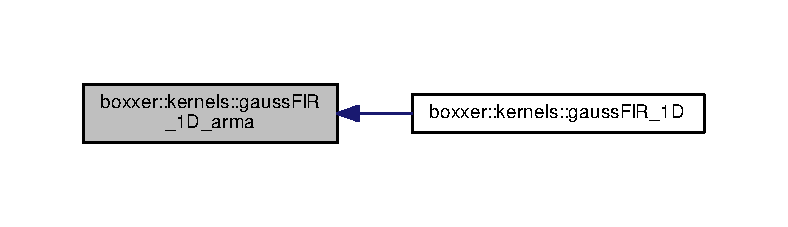
\includegraphics[width=350pt]{namespaceboxxer_1_1kernels_a88f298ecd82bf9083fabbb2e8a29d4e6_icgraph}
\end{center}
\end{figure}


\index{boxxer\+::kernels@{boxxer\+::kernels}!gauss\+F\+I\+R\+\_\+1\+D\+\_\+inplace@{gauss\+F\+I\+R\+\_\+1\+D\+\_\+inplace}}
\index{gauss\+F\+I\+R\+\_\+1\+D\+\_\+inplace@{gauss\+F\+I\+R\+\_\+1\+D\+\_\+inplace}!boxxer\+::kernels@{boxxer\+::kernels}}
\paragraph[{\texorpdfstring{gauss\+F\+I\+R\+\_\+1\+D\+\_\+inplace(\+Int\+T size, Float\+T data[], Int\+T hw, const Float\+T kernel[])}{gaussFIR_1D_inplace(IntT size, FloatT data[], IntT hw, const FloatT kernel[])}}]{\setlength{\rightskip}{0pt plus 5cm}template$<$class FloatT  = float, class IntT  = int32\+\_\+t$>$ void boxxer\+::kernels\+::gauss\+F\+I\+R\+\_\+1\+D\+\_\+inplace (
\begin{DoxyParamCaption}
\item[{IntT}]{size, }
\item[{FloatT}]{data\mbox{[}$\,$\mbox{]}, }
\item[{IntT}]{hw, }
\item[{const FloatT}]{kernel\mbox{[}$\,$\mbox{]}}
\end{DoxyParamCaption}
)}\hypertarget{namespaceboxxer_1_1kernels_ab3d9ad7bd61b25b9e856bd0284607e70}{}\label{namespaceboxxer_1_1kernels_ab3d9ad7bd61b25b9e856bd0284607e70}
This is details? 

Referenced by gauss\+F\+I\+R\+\_\+1\+D().



Here is the caller graph for this function\+:\nopagebreak
\begin{figure}[H]
\begin{center}
\leavevmode
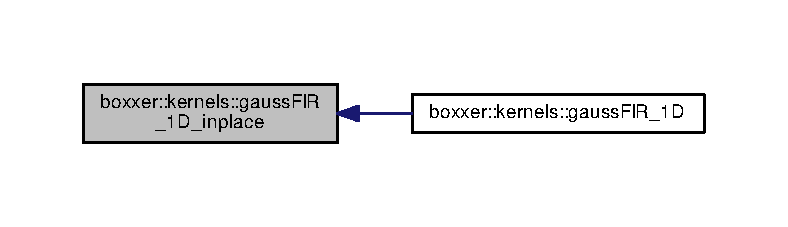
\includegraphics[width=350pt]{namespaceboxxer_1_1kernels_ab3d9ad7bd61b25b9e856bd0284607e70_icgraph}
\end{center}
\end{figure}


\index{boxxer\+::kernels@{boxxer\+::kernels}!gauss\+F\+I\+R\+\_\+1\+D\+\_\+inplace\+\_\+arma@{gauss\+F\+I\+R\+\_\+1\+D\+\_\+inplace\+\_\+arma}}
\index{gauss\+F\+I\+R\+\_\+1\+D\+\_\+inplace\+\_\+arma@{gauss\+F\+I\+R\+\_\+1\+D\+\_\+inplace\+\_\+arma}!boxxer\+::kernels@{boxxer\+::kernels}}
\paragraph[{\texorpdfstring{gauss\+F\+I\+R\+\_\+1\+D\+\_\+inplace\+\_\+arma(arma\+::\+Col$<$ Float\+T $>$ \&data, const arma\+::\+Col$<$ Float\+T $>$ \&kernel)}{gaussFIR_1D_inplace_arma(arma::Col< FloatT > &data, const arma::Col< FloatT > &kernel)}}]{\setlength{\rightskip}{0pt plus 5cm}template$<$class FloatT  = float, class IntT  = int32\+\_\+t$>$ void boxxer\+::kernels\+::gauss\+F\+I\+R\+\_\+1\+D\+\_\+inplace\+\_\+arma (
\begin{DoxyParamCaption}
\item[{arma\+::\+Col$<$ FloatT $>$ \&}]{data, }
\item[{const arma\+::\+Col$<$ FloatT $>$ \&}]{kernel}
\end{DoxyParamCaption}
)}\hypertarget{namespaceboxxer_1_1kernels_ab2a257fbea765aacf09b558e38637479}{}\label{namespaceboxxer_1_1kernels_ab2a257fbea765aacf09b558e38637479}
This is details? 

Referenced by gauss\+F\+I\+R\+\_\+1\+D().



Here is the caller graph for this function\+:\nopagebreak
\begin{figure}[H]
\begin{center}
\leavevmode
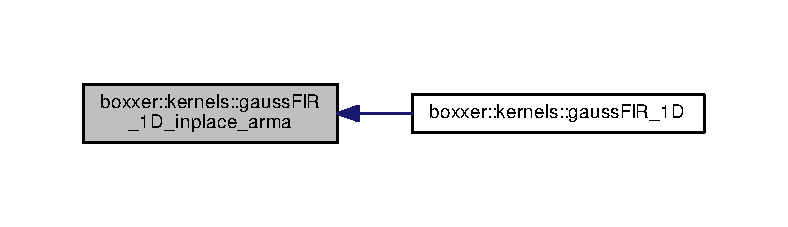
\includegraphics[width=350pt]{namespaceboxxer_1_1kernels_ab2a257fbea765aacf09b558e38637479_icgraph}
\end{center}
\end{figure}


\index{boxxer\+::kernels@{boxxer\+::kernels}!gauss\+F\+I\+R\+\_\+1\+D\+\_\+small@{gauss\+F\+I\+R\+\_\+1\+D\+\_\+small}}
\index{gauss\+F\+I\+R\+\_\+1\+D\+\_\+small@{gauss\+F\+I\+R\+\_\+1\+D\+\_\+small}!boxxer\+::kernels@{boxxer\+::kernels}}
\paragraph[{\texorpdfstring{gauss\+F\+I\+R\+\_\+1\+D\+\_\+small(\+Int\+T size, const Float\+T data[], Float\+T fdata[], Int\+T hw, const Float\+T kernel[])}{gaussFIR_1D_small(IntT size, const FloatT data[], FloatT fdata[], IntT hw, const FloatT kernel[])}}]{\setlength{\rightskip}{0pt plus 5cm}template$<$class FloatT  = float, class IntT  = int32\+\_\+t$>$ void boxxer\+::kernels\+::gauss\+F\+I\+R\+\_\+1\+D\+\_\+small (
\begin{DoxyParamCaption}
\item[{IntT}]{size, }
\item[{const FloatT}]{data\mbox{[}$\,$\mbox{]}, }
\item[{FloatT}]{fdata\mbox{[}$\,$\mbox{]}, }
\item[{IntT}]{hw, }
\item[{const FloatT}]{kernel\mbox{[}$\,$\mbox{]}}
\end{DoxyParamCaption}
)}\hypertarget{namespaceboxxer_1_1kernels_af07e73b62933910e86eef6b393155c2c}{}\label{namespaceboxxer_1_1kernels_af07e73b62933910e86eef6b393155c2c}
This is details? 

Referenced by gauss\+F\+I\+R\+\_\+1\+D().



Here is the caller graph for this function\+:\nopagebreak
\begin{figure}[H]
\begin{center}
\leavevmode
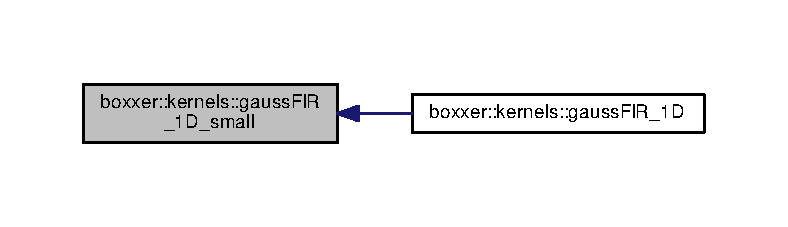
\includegraphics[width=350pt]{namespaceboxxer_1_1kernels_af07e73b62933910e86eef6b393155c2c_icgraph}
\end{center}
\end{figure}


\index{boxxer\+::kernels@{boxxer\+::kernels}!gauss\+F\+I\+R\+\_\+2\+Dx@{gauss\+F\+I\+R\+\_\+2\+Dx}}
\index{gauss\+F\+I\+R\+\_\+2\+Dx@{gauss\+F\+I\+R\+\_\+2\+Dx}!boxxer\+::kernels@{boxxer\+::kernels}}
\paragraph[{\texorpdfstring{gauss\+F\+I\+R\+\_\+2\+Dx(const arma\+::\+Mat$<$ Float\+T $>$ \&data, arma\+::\+Mat$<$ Float\+T $>$ \&fdata, const arma\+::\+Col$<$ Float\+T $>$ \&kernel)}{gaussFIR_2Dx(const arma::Mat< FloatT > &data, arma::Mat< FloatT > &fdata, const arma::Col< FloatT > &kernel)}}]{\setlength{\rightskip}{0pt plus 5cm}template$<$class FloatT  = float, class IntT  = int32\+\_\+t$>$ void boxxer\+::kernels\+::gauss\+F\+I\+R\+\_\+2\+Dx (
\begin{DoxyParamCaption}
\item[{const arma\+::\+Mat$<$ FloatT $>$ \&}]{data, }
\item[{arma\+::\+Mat$<$ FloatT $>$ \&}]{fdata, }
\item[{const arma\+::\+Col$<$ FloatT $>$ \&}]{kernel}
\end{DoxyParamCaption}
)}\hypertarget{namespaceboxxer_1_1kernels_aeee9d632ce320eb89c870a44c37efa65}{}\label{namespaceboxxer_1_1kernels_aeee9d632ce320eb89c870a44c37efa65}
2D Gauss F\+IR Filters 

Referenced by gauss\+F\+I\+R\+\_\+1\+D().



Here is the caller graph for this function\+:\nopagebreak
\begin{figure}[H]
\begin{center}
\leavevmode
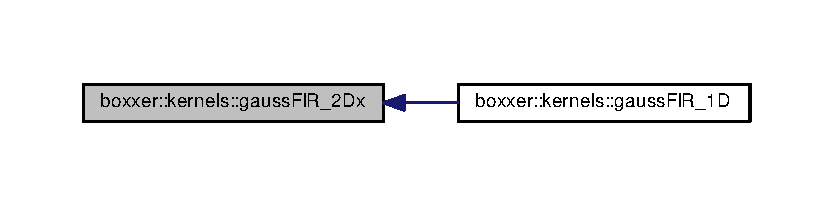
\includegraphics[width=350pt]{namespaceboxxer_1_1kernels_aeee9d632ce320eb89c870a44c37efa65_icgraph}
\end{center}
\end{figure}


\index{boxxer\+::kernels@{boxxer\+::kernels}!gauss\+F\+I\+R\+\_\+2\+Dx\+\_\+arma@{gauss\+F\+I\+R\+\_\+2\+Dx\+\_\+arma}}
\index{gauss\+F\+I\+R\+\_\+2\+Dx\+\_\+arma@{gauss\+F\+I\+R\+\_\+2\+Dx\+\_\+arma}!boxxer\+::kernels@{boxxer\+::kernels}}
\paragraph[{\texorpdfstring{gauss\+F\+I\+R\+\_\+2\+Dx\+\_\+arma(const arma\+::\+Mat$<$ Float\+T $>$ \&data, arma\+::\+Mat$<$ Float\+T $>$ \&fdata, const arma\+::\+Col$<$ Float\+T $>$ \&kernel)}{gaussFIR_2Dx_arma(const arma::Mat< FloatT > &data, arma::Mat< FloatT > &fdata, const arma::Col< FloatT > &kernel)}}]{\setlength{\rightskip}{0pt plus 5cm}template$<$class FloatT  = float, class IntT  = int32\+\_\+t$>$ void boxxer\+::kernels\+::gauss\+F\+I\+R\+\_\+2\+Dx\+\_\+arma (
\begin{DoxyParamCaption}
\item[{const arma\+::\+Mat$<$ FloatT $>$ \&}]{data, }
\item[{arma\+::\+Mat$<$ FloatT $>$ \&}]{fdata, }
\item[{const arma\+::\+Col$<$ FloatT $>$ \&}]{kernel}
\end{DoxyParamCaption}
)}\hypertarget{namespaceboxxer_1_1kernels_a1da855e7008385fee013bd868d206040}{}\label{namespaceboxxer_1_1kernels_a1da855e7008385fee013bd868d206040}
2D Gauss F\+IR Filters 

Referenced by gauss\+F\+I\+R\+\_\+1\+D().



Here is the caller graph for this function\+:\nopagebreak
\begin{figure}[H]
\begin{center}
\leavevmode
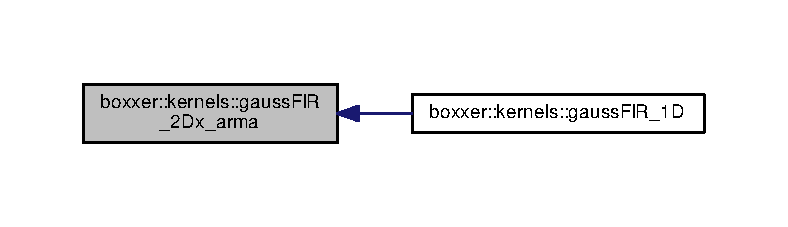
\includegraphics[width=350pt]{namespaceboxxer_1_1kernels_a1da855e7008385fee013bd868d206040_icgraph}
\end{center}
\end{figure}


\index{boxxer\+::kernels@{boxxer\+::kernels}!gauss\+F\+I\+R\+\_\+2\+Dx\+\_\+small@{gauss\+F\+I\+R\+\_\+2\+Dx\+\_\+small}}
\index{gauss\+F\+I\+R\+\_\+2\+Dx\+\_\+small@{gauss\+F\+I\+R\+\_\+2\+Dx\+\_\+small}!boxxer\+::kernels@{boxxer\+::kernels}}
\paragraph[{\texorpdfstring{gauss\+F\+I\+R\+\_\+2\+Dx\+\_\+small(const arma\+::\+Mat$<$ Float\+T $>$ \&data, arma\+::\+Mat$<$ Float\+T $>$ \&fdata, const arma\+::\+Col$<$ Float\+T $>$ \&kernel)}{gaussFIR_2Dx_small(const arma::Mat< FloatT > &data, arma::Mat< FloatT > &fdata, const arma::Col< FloatT > &kernel)}}]{\setlength{\rightskip}{0pt plus 5cm}template$<$class FloatT  = float, class IntT  = int32\+\_\+t$>$ void boxxer\+::kernels\+::gauss\+F\+I\+R\+\_\+2\+Dx\+\_\+small (
\begin{DoxyParamCaption}
\item[{const arma\+::\+Mat$<$ FloatT $>$ \&}]{data, }
\item[{arma\+::\+Mat$<$ FloatT $>$ \&}]{fdata, }
\item[{const arma\+::\+Col$<$ FloatT $>$ \&}]{kernel}
\end{DoxyParamCaption}
)}\hypertarget{namespaceboxxer_1_1kernels_a638bf7fa9900937a763f190c0a4499ae}{}\label{namespaceboxxer_1_1kernels_a638bf7fa9900937a763f190c0a4499ae}
2D Gauss F\+IR Filters 

Referenced by gauss\+F\+I\+R\+\_\+1\+D().



Here is the caller graph for this function\+:\nopagebreak
\begin{figure}[H]
\begin{center}
\leavevmode
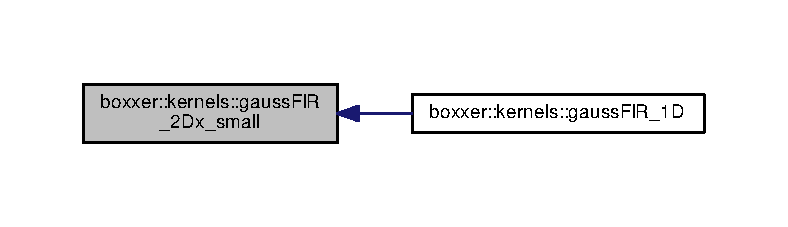
\includegraphics[width=350pt]{namespaceboxxer_1_1kernels_a638bf7fa9900937a763f190c0a4499ae_icgraph}
\end{center}
\end{figure}


\index{boxxer\+::kernels@{boxxer\+::kernels}!gauss\+F\+I\+R\+\_\+2\+Dy@{gauss\+F\+I\+R\+\_\+2\+Dy}}
\index{gauss\+F\+I\+R\+\_\+2\+Dy@{gauss\+F\+I\+R\+\_\+2\+Dy}!boxxer\+::kernels@{boxxer\+::kernels}}
\paragraph[{\texorpdfstring{gauss\+F\+I\+R\+\_\+2\+Dy(const arma\+::\+Mat$<$ Float\+T $>$ \&data, arma\+::\+Mat$<$ Float\+T $>$ \&fdata, const arma\+::\+Col$<$ Float\+T $>$ \&kernel)}{gaussFIR_2Dy(const arma::Mat< FloatT > &data, arma::Mat< FloatT > &fdata, const arma::Col< FloatT > &kernel)}}]{\setlength{\rightskip}{0pt plus 5cm}template$<$class FloatT  = float, class IntT  = int32\+\_\+t$>$ void boxxer\+::kernels\+::gauss\+F\+I\+R\+\_\+2\+Dy (
\begin{DoxyParamCaption}
\item[{const arma\+::\+Mat$<$ FloatT $>$ \&}]{data, }
\item[{arma\+::\+Mat$<$ FloatT $>$ \&}]{fdata, }
\item[{const arma\+::\+Col$<$ FloatT $>$ \&}]{kernel}
\end{DoxyParamCaption}
)}\hypertarget{namespaceboxxer_1_1kernels_a6efa0d22ae67955f27c6d9ea30342104}{}\label{namespaceboxxer_1_1kernels_a6efa0d22ae67955f27c6d9ea30342104}
2D Gauss F\+IR Filters 

Referenced by gauss\+F\+I\+R\+\_\+1\+D().



Here is the caller graph for this function\+:\nopagebreak
\begin{figure}[H]
\begin{center}
\leavevmode
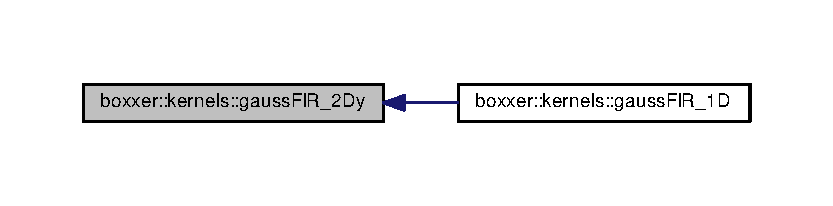
\includegraphics[width=350pt]{namespaceboxxer_1_1kernels_a6efa0d22ae67955f27c6d9ea30342104_icgraph}
\end{center}
\end{figure}


\index{boxxer\+::kernels@{boxxer\+::kernels}!gauss\+F\+I\+R\+\_\+2\+Dy\+\_\+colmajor@{gauss\+F\+I\+R\+\_\+2\+Dy\+\_\+colmajor}}
\index{gauss\+F\+I\+R\+\_\+2\+Dy\+\_\+colmajor@{gauss\+F\+I\+R\+\_\+2\+Dy\+\_\+colmajor}!boxxer\+::kernels@{boxxer\+::kernels}}
\paragraph[{\texorpdfstring{gauss\+F\+I\+R\+\_\+2\+Dy\+\_\+colmajor(const arma\+::\+Mat$<$ Float\+T $>$ \&data, arma\+::\+Mat$<$ Float\+T $>$ \&fdata, const arma\+::\+Col$<$ Float\+T $>$ \&kernel)}{gaussFIR_2Dy_colmajor(const arma::Mat< FloatT > &data, arma::Mat< FloatT > &fdata, const arma::Col< FloatT > &kernel)}}]{\setlength{\rightskip}{0pt plus 5cm}template$<$class FloatT  = float, class IntT  = int32\+\_\+t$>$ void boxxer\+::kernels\+::gauss\+F\+I\+R\+\_\+2\+Dy\+\_\+colmajor (
\begin{DoxyParamCaption}
\item[{const arma\+::\+Mat$<$ FloatT $>$ \&}]{data, }
\item[{arma\+::\+Mat$<$ FloatT $>$ \&}]{fdata, }
\item[{const arma\+::\+Col$<$ FloatT $>$ \&}]{kernel}
\end{DoxyParamCaption}
)}\hypertarget{namespaceboxxer_1_1kernels_ae78e8767ae044f01e07e61a45220ffc5}{}\label{namespaceboxxer_1_1kernels_ae78e8767ae044f01e07e61a45220ffc5}
2D Gauss F\+IR Filters 

Referenced by gauss\+F\+I\+R\+\_\+1\+D().



Here is the caller graph for this function\+:\nopagebreak
\begin{figure}[H]
\begin{center}
\leavevmode
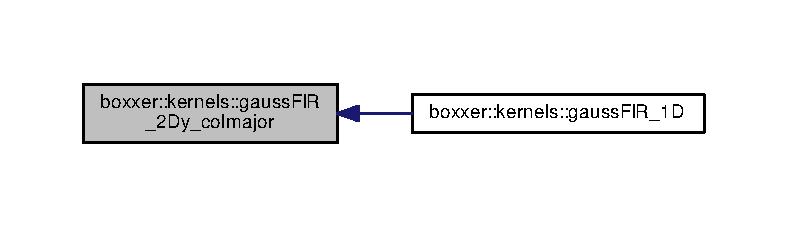
\includegraphics[width=350pt]{namespaceboxxer_1_1kernels_ae78e8767ae044f01e07e61a45220ffc5_icgraph}
\end{center}
\end{figure}


\index{boxxer\+::kernels@{boxxer\+::kernels}!gauss\+F\+I\+R\+\_\+2\+Dy\+\_\+rowmajor@{gauss\+F\+I\+R\+\_\+2\+Dy\+\_\+rowmajor}}
\index{gauss\+F\+I\+R\+\_\+2\+Dy\+\_\+rowmajor@{gauss\+F\+I\+R\+\_\+2\+Dy\+\_\+rowmajor}!boxxer\+::kernels@{boxxer\+::kernels}}
\paragraph[{\texorpdfstring{gauss\+F\+I\+R\+\_\+2\+Dy\+\_\+rowmajor(const arma\+::\+Mat$<$ Float\+T $>$ \&data, arma\+::\+Mat$<$ Float\+T $>$ \&fdata, const arma\+::\+Col$<$ Float\+T $>$ \&kernel)}{gaussFIR_2Dy_rowmajor(const arma::Mat< FloatT > &data, arma::Mat< FloatT > &fdata, const arma::Col< FloatT > &kernel)}}]{\setlength{\rightskip}{0pt plus 5cm}template$<$class FloatT  = float, class IntT  = int32\+\_\+t$>$ void boxxer\+::kernels\+::gauss\+F\+I\+R\+\_\+2\+Dy\+\_\+rowmajor (
\begin{DoxyParamCaption}
\item[{const arma\+::\+Mat$<$ FloatT $>$ \&}]{data, }
\item[{arma\+::\+Mat$<$ FloatT $>$ \&}]{fdata, }
\item[{const arma\+::\+Col$<$ FloatT $>$ \&}]{kernel}
\end{DoxyParamCaption}
)}\hypertarget{namespaceboxxer_1_1kernels_aa54bb3fea2d343c030528a87b7916293}{}\label{namespaceboxxer_1_1kernels_aa54bb3fea2d343c030528a87b7916293}
2D Gauss F\+IR Filters 

Referenced by gauss\+F\+I\+R\+\_\+1\+D().



Here is the caller graph for this function\+:\nopagebreak
\begin{figure}[H]
\begin{center}
\leavevmode
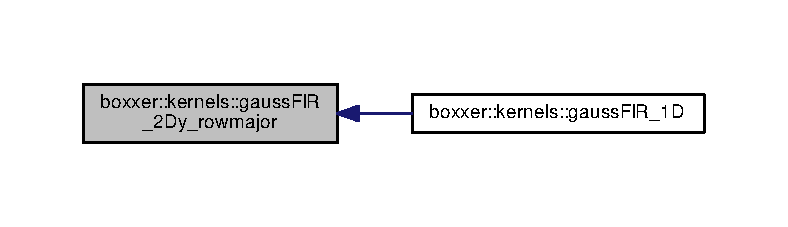
\includegraphics[width=350pt]{namespaceboxxer_1_1kernels_aa54bb3fea2d343c030528a87b7916293_icgraph}
\end{center}
\end{figure}


\index{boxxer\+::kernels@{boxxer\+::kernels}!gauss\+F\+I\+R\+\_\+2\+Dy\+\_\+small@{gauss\+F\+I\+R\+\_\+2\+Dy\+\_\+small}}
\index{gauss\+F\+I\+R\+\_\+2\+Dy\+\_\+small@{gauss\+F\+I\+R\+\_\+2\+Dy\+\_\+small}!boxxer\+::kernels@{boxxer\+::kernels}}
\paragraph[{\texorpdfstring{gauss\+F\+I\+R\+\_\+2\+Dy\+\_\+small(const arma\+::\+Mat$<$ Float\+T $>$ \&data, arma\+::\+Mat$<$ Float\+T $>$ \&fdata, const arma\+::\+Col$<$ Float\+T $>$ \&kernel)}{gaussFIR_2Dy_small(const arma::Mat< FloatT > &data, arma::Mat< FloatT > &fdata, const arma::Col< FloatT > &kernel)}}]{\setlength{\rightskip}{0pt plus 5cm}template$<$class FloatT  = float, class IntT  = int32\+\_\+t$>$ void boxxer\+::kernels\+::gauss\+F\+I\+R\+\_\+2\+Dy\+\_\+small (
\begin{DoxyParamCaption}
\item[{const arma\+::\+Mat$<$ FloatT $>$ \&}]{data, }
\item[{arma\+::\+Mat$<$ FloatT $>$ \&}]{fdata, }
\item[{const arma\+::\+Col$<$ FloatT $>$ \&}]{kernel}
\end{DoxyParamCaption}
)}\hypertarget{namespaceboxxer_1_1kernels_a49fd7ed785cfcea57b4c9e67d3113a69}{}\label{namespaceboxxer_1_1kernels_a49fd7ed785cfcea57b4c9e67d3113a69}
2D Gauss F\+IR Filters 

Referenced by gauss\+F\+I\+R\+\_\+1\+D().



Here is the caller graph for this function\+:\nopagebreak
\begin{figure}[H]
\begin{center}
\leavevmode
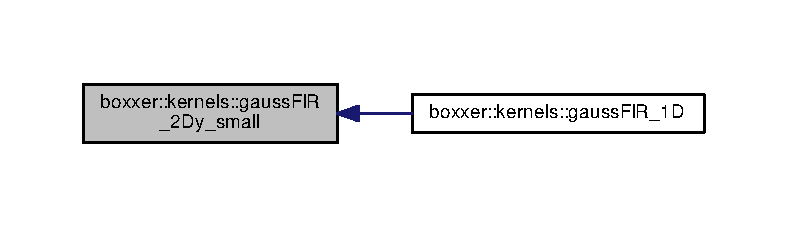
\includegraphics[width=350pt]{namespaceboxxer_1_1kernels_a49fd7ed785cfcea57b4c9e67d3113a69_icgraph}
\end{center}
\end{figure}


\index{boxxer\+::kernels@{boxxer\+::kernels}!gauss\+F\+I\+R\+\_\+3\+Dx@{gauss\+F\+I\+R\+\_\+3\+Dx}}
\index{gauss\+F\+I\+R\+\_\+3\+Dx@{gauss\+F\+I\+R\+\_\+3\+Dx}!boxxer\+::kernels@{boxxer\+::kernels}}
\paragraph[{\texorpdfstring{gauss\+F\+I\+R\+\_\+3\+Dx(const arma\+::\+Cube$<$ Float\+T $>$ \&data, arma\+::\+Cube$<$ Float\+T $>$ \&fdata, const arma\+::\+Col$<$ Float\+T $>$ \&kernel)}{gaussFIR_3Dx(const arma::Cube< FloatT > &data, arma::Cube< FloatT > &fdata, const arma::Col< FloatT > &kernel)}}]{\setlength{\rightskip}{0pt plus 5cm}template$<$class FloatT  = float, class IntT  = int32\+\_\+t$>$ void boxxer\+::kernels\+::gauss\+F\+I\+R\+\_\+3\+Dx (
\begin{DoxyParamCaption}
\item[{const arma\+::\+Cube$<$ FloatT $>$ \&}]{data, }
\item[{arma\+::\+Cube$<$ FloatT $>$ \&}]{fdata, }
\item[{const arma\+::\+Col$<$ FloatT $>$ \&}]{kernel}
\end{DoxyParamCaption}
)}\hypertarget{namespaceboxxer_1_1kernels_a74811c999b7d18b14dde0a042318fc06}{}\label{namespaceboxxer_1_1kernels_a74811c999b7d18b14dde0a042318fc06}
3D Gauss F\+IR Filters 

Referenced by gauss\+F\+I\+R\+\_\+1\+D().



Here is the caller graph for this function\+:\nopagebreak
\begin{figure}[H]
\begin{center}
\leavevmode
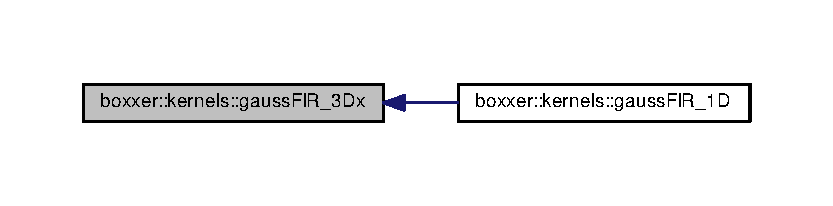
\includegraphics[width=350pt]{namespaceboxxer_1_1kernels_a74811c999b7d18b14dde0a042318fc06_icgraph}
\end{center}
\end{figure}


\index{boxxer\+::kernels@{boxxer\+::kernels}!gauss\+F\+I\+R\+\_\+3\+Dx\+\_\+small@{gauss\+F\+I\+R\+\_\+3\+Dx\+\_\+small}}
\index{gauss\+F\+I\+R\+\_\+3\+Dx\+\_\+small@{gauss\+F\+I\+R\+\_\+3\+Dx\+\_\+small}!boxxer\+::kernels@{boxxer\+::kernels}}
\paragraph[{\texorpdfstring{gauss\+F\+I\+R\+\_\+3\+Dx\+\_\+small(const arma\+::\+Cube$<$ Float\+T $>$ \&data, arma\+::\+Cube$<$ Float\+T $>$ \&fdata, const arma\+::\+Col$<$ Float\+T $>$ \&kernel)}{gaussFIR_3Dx_small(const arma::Cube< FloatT > &data, arma::Cube< FloatT > &fdata, const arma::Col< FloatT > &kernel)}}]{\setlength{\rightskip}{0pt plus 5cm}template$<$class FloatT  = float, class IntT  = int32\+\_\+t$>$ void boxxer\+::kernels\+::gauss\+F\+I\+R\+\_\+3\+Dx\+\_\+small (
\begin{DoxyParamCaption}
\item[{const arma\+::\+Cube$<$ FloatT $>$ \&}]{data, }
\item[{arma\+::\+Cube$<$ FloatT $>$ \&}]{fdata, }
\item[{const arma\+::\+Col$<$ FloatT $>$ \&}]{kernel}
\end{DoxyParamCaption}
)}\hypertarget{namespaceboxxer_1_1kernels_af7d8fb262d8bde9c9907e141c3c5f55f}{}\label{namespaceboxxer_1_1kernels_af7d8fb262d8bde9c9907e141c3c5f55f}
3D Gauss F\+IR Filters 

Referenced by gauss\+F\+I\+R\+\_\+1\+D().



Here is the caller graph for this function\+:\nopagebreak
\begin{figure}[H]
\begin{center}
\leavevmode
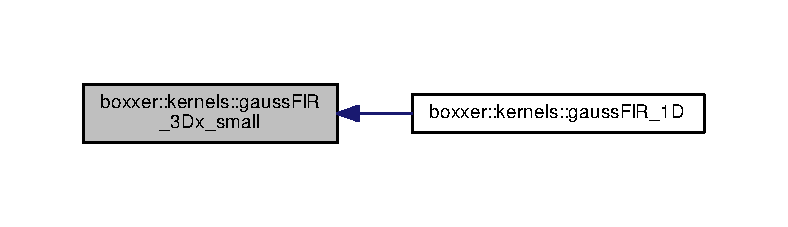
\includegraphics[width=350pt]{namespaceboxxer_1_1kernels_af7d8fb262d8bde9c9907e141c3c5f55f_icgraph}
\end{center}
\end{figure}


\index{boxxer\+::kernels@{boxxer\+::kernels}!gauss\+F\+I\+R\+\_\+3\+Dy@{gauss\+F\+I\+R\+\_\+3\+Dy}}
\index{gauss\+F\+I\+R\+\_\+3\+Dy@{gauss\+F\+I\+R\+\_\+3\+Dy}!boxxer\+::kernels@{boxxer\+::kernels}}
\paragraph[{\texorpdfstring{gauss\+F\+I\+R\+\_\+3\+Dy(const arma\+::\+Cube$<$ Float\+T $>$ \&data, arma\+::\+Cube$<$ Float\+T $>$ \&fdata, const arma\+::\+Col$<$ Float\+T $>$ \&kernel)}{gaussFIR_3Dy(const arma::Cube< FloatT > &data, arma::Cube< FloatT > &fdata, const arma::Col< FloatT > &kernel)}}]{\setlength{\rightskip}{0pt plus 5cm}template$<$class FloatT  = float, class IntT  = int32\+\_\+t$>$ void boxxer\+::kernels\+::gauss\+F\+I\+R\+\_\+3\+Dy (
\begin{DoxyParamCaption}
\item[{const arma\+::\+Cube$<$ FloatT $>$ \&}]{data, }
\item[{arma\+::\+Cube$<$ FloatT $>$ \&}]{fdata, }
\item[{const arma\+::\+Col$<$ FloatT $>$ \&}]{kernel}
\end{DoxyParamCaption}
)}\hypertarget{namespaceboxxer_1_1kernels_ac97f85b9211fcffa432b44a86d30c5df}{}\label{namespaceboxxer_1_1kernels_ac97f85b9211fcffa432b44a86d30c5df}
3D Gauss F\+IR Filters 

Referenced by gauss\+F\+I\+R\+\_\+1\+D().



Here is the caller graph for this function\+:\nopagebreak
\begin{figure}[H]
\begin{center}
\leavevmode
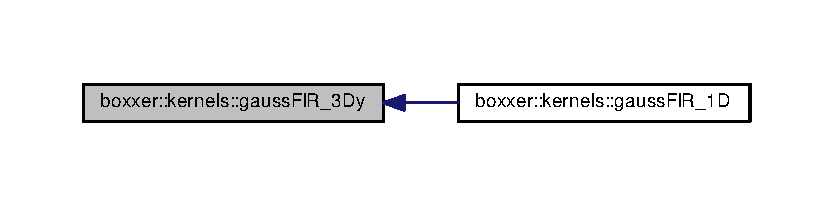
\includegraphics[width=350pt]{namespaceboxxer_1_1kernels_ac97f85b9211fcffa432b44a86d30c5df_icgraph}
\end{center}
\end{figure}


\index{boxxer\+::kernels@{boxxer\+::kernels}!gauss\+F\+I\+R\+\_\+3\+Dy\+\_\+small@{gauss\+F\+I\+R\+\_\+3\+Dy\+\_\+small}}
\index{gauss\+F\+I\+R\+\_\+3\+Dy\+\_\+small@{gauss\+F\+I\+R\+\_\+3\+Dy\+\_\+small}!boxxer\+::kernels@{boxxer\+::kernels}}
\paragraph[{\texorpdfstring{gauss\+F\+I\+R\+\_\+3\+Dy\+\_\+small(const arma\+::\+Cube$<$ Float\+T $>$ \&data, arma\+::\+Cube$<$ Float\+T $>$ \&fdata, const arma\+::\+Col$<$ Float\+T $>$ \&kernel)}{gaussFIR_3Dy_small(const arma::Cube< FloatT > &data, arma::Cube< FloatT > &fdata, const arma::Col< FloatT > &kernel)}}]{\setlength{\rightskip}{0pt plus 5cm}template$<$class FloatT  = float, class IntT  = int32\+\_\+t$>$ void boxxer\+::kernels\+::gauss\+F\+I\+R\+\_\+3\+Dy\+\_\+small (
\begin{DoxyParamCaption}
\item[{const arma\+::\+Cube$<$ FloatT $>$ \&}]{data, }
\item[{arma\+::\+Cube$<$ FloatT $>$ \&}]{fdata, }
\item[{const arma\+::\+Col$<$ FloatT $>$ \&}]{kernel}
\end{DoxyParamCaption}
)}\hypertarget{namespaceboxxer_1_1kernels_a0256b4053077d18bbe2228402071555f}{}\label{namespaceboxxer_1_1kernels_a0256b4053077d18bbe2228402071555f}
3D Gauss F\+IR Filters 

Referenced by gauss\+F\+I\+R\+\_\+1\+D().



Here is the caller graph for this function\+:\nopagebreak
\begin{figure}[H]
\begin{center}
\leavevmode
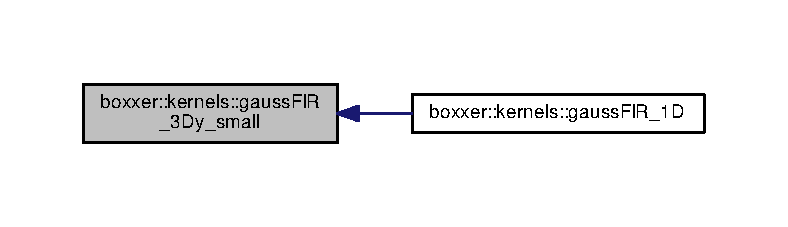
\includegraphics[width=350pt]{namespaceboxxer_1_1kernels_a0256b4053077d18bbe2228402071555f_icgraph}
\end{center}
\end{figure}


\index{boxxer\+::kernels@{boxxer\+::kernels}!gauss\+F\+I\+R\+\_\+3\+Dz@{gauss\+F\+I\+R\+\_\+3\+Dz}}
\index{gauss\+F\+I\+R\+\_\+3\+Dz@{gauss\+F\+I\+R\+\_\+3\+Dz}!boxxer\+::kernels@{boxxer\+::kernels}}
\paragraph[{\texorpdfstring{gauss\+F\+I\+R\+\_\+3\+Dz(const arma\+::\+Cube$<$ Float\+T $>$ \&data, arma\+::\+Cube$<$ Float\+T $>$ \&fdata, const arma\+::\+Col$<$ Float\+T $>$ \&kernel)}{gaussFIR_3Dz(const arma::Cube< FloatT > &data, arma::Cube< FloatT > &fdata, const arma::Col< FloatT > &kernel)}}]{\setlength{\rightskip}{0pt plus 5cm}template$<$class FloatT  = float, class IntT  = int32\+\_\+t$>$ void boxxer\+::kernels\+::gauss\+F\+I\+R\+\_\+3\+Dz (
\begin{DoxyParamCaption}
\item[{const arma\+::\+Cube$<$ FloatT $>$ \&}]{data, }
\item[{arma\+::\+Cube$<$ FloatT $>$ \&}]{fdata, }
\item[{const arma\+::\+Col$<$ FloatT $>$ \&}]{kernel}
\end{DoxyParamCaption}
)}\hypertarget{namespaceboxxer_1_1kernels_a404ef6e2324a0e4ff53e38ad7b07733e}{}\label{namespaceboxxer_1_1kernels_a404ef6e2324a0e4ff53e38ad7b07733e}
3D Gauss F\+IR Filters 

Referenced by gauss\+F\+I\+R\+\_\+1\+D().



Here is the caller graph for this function\+:\nopagebreak
\begin{figure}[H]
\begin{center}
\leavevmode
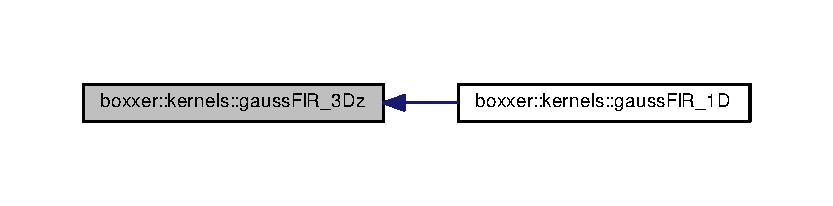
\includegraphics[width=350pt]{namespaceboxxer_1_1kernels_a404ef6e2324a0e4ff53e38ad7b07733e_icgraph}
\end{center}
\end{figure}


\index{boxxer\+::kernels@{boxxer\+::kernels}!gauss\+F\+I\+R\+\_\+3\+Dz\+\_\+small@{gauss\+F\+I\+R\+\_\+3\+Dz\+\_\+small}}
\index{gauss\+F\+I\+R\+\_\+3\+Dz\+\_\+small@{gauss\+F\+I\+R\+\_\+3\+Dz\+\_\+small}!boxxer\+::kernels@{boxxer\+::kernels}}
\paragraph[{\texorpdfstring{gauss\+F\+I\+R\+\_\+3\+Dz\+\_\+small(const arma\+::\+Cube$<$ Float\+T $>$ \&data, arma\+::\+Cube$<$ Float\+T $>$ \&fdata, const arma\+::\+Col$<$ Float\+T $>$ \&kernel)}{gaussFIR_3Dz_small(const arma::Cube< FloatT > &data, arma::Cube< FloatT > &fdata, const arma::Col< FloatT > &kernel)}}]{\setlength{\rightskip}{0pt plus 5cm}template$<$class FloatT  = float, class IntT  = int32\+\_\+t$>$ void boxxer\+::kernels\+::gauss\+F\+I\+R\+\_\+3\+Dz\+\_\+small (
\begin{DoxyParamCaption}
\item[{const arma\+::\+Cube$<$ FloatT $>$ \&}]{data, }
\item[{arma\+::\+Cube$<$ FloatT $>$ \&}]{fdata, }
\item[{const arma\+::\+Col$<$ FloatT $>$ \&}]{kernel}
\end{DoxyParamCaption}
)}\hypertarget{namespaceboxxer_1_1kernels_a9a9201ede570bb2d77531d529f39bc99}{}\label{namespaceboxxer_1_1kernels_a9a9201ede570bb2d77531d529f39bc99}
3D Gauss F\+IR Filters 

Referenced by gauss\+F\+I\+R\+\_\+1\+D().



Here is the caller graph for this function\+:\nopagebreak
\begin{figure}[H]
\begin{center}
\leavevmode
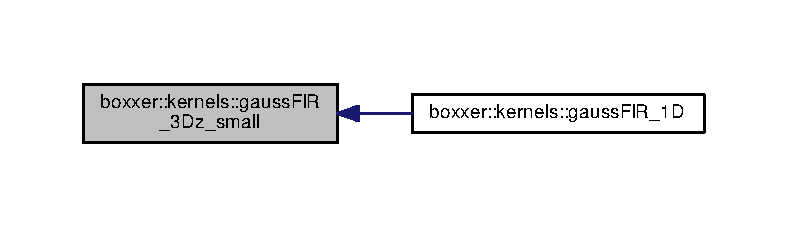
\includegraphics[width=350pt]{namespaceboxxer_1_1kernels_a9a9201ede570bb2d77531d529f39bc99_icgraph}
\end{center}
\end{figure}



\section{Class Documentation}
\hypertarget{classboxxer_1_1Boxxer2D}{}\subsection{boxxer\+:\+:Boxxer2D$<$ FloatT, IdxT $>$ Class Template Reference}
\label{classboxxer_1_1Boxxer2D}\index{boxxer\+::\+Boxxer2\+D$<$ Float\+T, Idx\+T $>$@{boxxer\+::\+Boxxer2\+D$<$ Float\+T, Idx\+T $>$}}


{\ttfamily \#include $<$/home/travis/build/markjolah/\+Boxxer/include/\+Boxxer/\+Boxxer2\+D.\+h$>$}

\subsubsection*{Public Types}
\begin{DoxyCompactItemize}
\item 
using \hyperlink{classboxxer_1_1Boxxer2D_acb4dc89c7e1bd2099e7de7b83621ba4f}{I\+VecT} = arma\+::\+Col$<$ IdxT $>$
\item 
using \hyperlink{classboxxer_1_1Boxxer2D_ad6e571d3e7685b8c634661e03382a32f}{I\+MatT} = arma\+::\+Mat$<$ IdxT $>$
\item 
using \hyperlink{classboxxer_1_1Boxxer2D_aeb45bfe57b8975660fc7076a2794acf8}{VecT} = arma\+::\+Col$<$ FloatT $>$
\item 
using \hyperlink{classboxxer_1_1Boxxer2D_a4af9f3e10a7ceb1c20e1d731263d9aeb}{MatT} = arma\+::\+Mat$<$ FloatT $>$
\item 
using \hyperlink{classboxxer_1_1Boxxer2D_ad1c52f05a957159bf373b4d8c4361ffe}{ImageT} = arma\+::\+Mat$<$ FloatT $>$
\item 
using \hyperlink{classboxxer_1_1Boxxer2D_a35da86be183f5f24cb3d13cbf7cf45ee}{Image\+StackT} = arma\+::\+Cube$<$ FloatT $>$
\item 
using \hyperlink{classboxxer_1_1Boxxer2D_ad8d3ac7a59998612e4ce00500416c8c1}{Scaled\+ImageT} = arma\+::\+Cube$<$ FloatT $>$
\item 
using \hyperlink{classboxxer_1_1Boxxer2D_a2937a772edcf9cec5f617fbcf1d8a6fe}{Scaled\+Image\+StackT} = hypercube\+::\+Hypercube$<$ FloatT $>$
\end{DoxyCompactItemize}
\subsubsection*{Public Member Functions}
\begin{DoxyCompactItemize}
\item 
\hyperlink{classboxxer_1_1Boxxer2D_a9f87f606cf304f6006d055ef20d25f73}{Boxxer2D} (const \hyperlink{classboxxer_1_1Boxxer2D_acb4dc89c7e1bd2099e7de7b83621ba4f}{I\+VecT} \&\hyperlink{classboxxer_1_1Boxxer2D_a6f76692e32f0c907d48a72a801a62b9a}{imsize}, const \hyperlink{classboxxer_1_1Boxxer2D_a4af9f3e10a7ceb1c20e1d731263d9aeb}{MatT} \&\hyperlink{classboxxer_1_1Boxxer2D_a925fe4151cca3a34cba36f1a10b8e382}{sigma})
\item 
void \hyperlink{classboxxer_1_1Boxxer2D_a9fcfdebe9f2896232c50b482005db219}{set\+Do\+G\+Sigma\+Ratio} (FloatT \hyperlink{classboxxer_1_1Boxxer2D_a0fffedee4a39644c5c48fba99e297111}{sigma\+\_\+ratio})
\item 
void \hyperlink{classboxxer_1_1Boxxer2D_a3291815bf3f9a0762f542bfe636b6da4}{filter\+Scaled\+LoG} (const \hyperlink{classboxxer_1_1Boxxer2D_a35da86be183f5f24cb3d13cbf7cf45ee}{Image\+StackT} \&im, \hyperlink{classboxxer_1_1Boxxer2D_a2937a772edcf9cec5f617fbcf1d8a6fe}{Scaled\+Image\+StackT} \&fim) const 
\item 
void \hyperlink{classboxxer_1_1Boxxer2D_a35393374b3c73f09c7a6a4a45ec82856}{filter\+Scaled\+DoG} (const \hyperlink{classboxxer_1_1Boxxer2D_a35da86be183f5f24cb3d13cbf7cf45ee}{Image\+StackT} \&im, \hyperlink{classboxxer_1_1Boxxer2D_a2937a772edcf9cec5f617fbcf1d8a6fe}{Scaled\+Image\+StackT} \&fim) const 
\item 
IdxT \hyperlink{classboxxer_1_1Boxxer2D_ad5dffcdf4797f49541b9c44c9551987a}{scale\+Space\+Lo\+G\+Maxima} (const \hyperlink{classboxxer_1_1Boxxer2D_a35da86be183f5f24cb3d13cbf7cf45ee}{Image\+StackT} \&im, \hyperlink{classboxxer_1_1Boxxer2D_ad6e571d3e7685b8c634661e03382a32f}{I\+MatT} \&maxima, \hyperlink{classboxxer_1_1Boxxer2D_aeb45bfe57b8975660fc7076a2794acf8}{VecT} \&max\+\_\+vals, IdxT neighborhood\+\_\+size, IdxT scale\+\_\+neighborhood\+\_\+size) const 
\item 
IdxT \hyperlink{classboxxer_1_1Boxxer2D_ad3d93a33dcef252f4f0be57a27535f6e}{scale\+Space\+Do\+G\+Maxima} (const \hyperlink{classboxxer_1_1Boxxer2D_a35da86be183f5f24cb3d13cbf7cf45ee}{Image\+StackT} \&im, \hyperlink{classboxxer_1_1Boxxer2D_ad6e571d3e7685b8c634661e03382a32f}{I\+MatT} \&maxima, \hyperlink{classboxxer_1_1Boxxer2D_aeb45bfe57b8975660fc7076a2794acf8}{VecT} \&max\+\_\+vals, IdxT neighborhood\+\_\+size, IdxT scale\+\_\+neighborhood\+\_\+size) const 
\item 
\hyperlink{classboxxer_1_1Boxxer2D_ad1c52f05a957159bf373b4d8c4361ffe}{ImageT} \hyperlink{classboxxer_1_1Boxxer2D_a3a3deae8a4d6105bcf5793151278f9b7}{make\+\_\+image} () const 
\item 
\hyperlink{classboxxer_1_1Boxxer2D_a35da86be183f5f24cb3d13cbf7cf45ee}{Image\+StackT} \hyperlink{classboxxer_1_1Boxxer2D_aa481bbbab9b8aff1f470a5c82fb71f9b}{make\+\_\+image\+\_\+stack} (IdxT nT) const 
\item 
\hyperlink{classboxxer_1_1Boxxer2D_ad8d3ac7a59998612e4ce00500416c8c1}{Scaled\+ImageT} \hyperlink{classboxxer_1_1Boxxer2D_a4817f3e6707a0ca9330ae6f0dbfb89da}{make\+\_\+scaled\+\_\+image} () const 
\item 
\hyperlink{classboxxer_1_1Boxxer2D_a2937a772edcf9cec5f617fbcf1d8a6fe}{Scaled\+Image\+StackT} \hyperlink{classboxxer_1_1Boxxer2D_a5c2ee267ed5ac1c61d3b7a9c935e0922}{make\+\_\+scaled\+\_\+image\+\_\+stack} (IdxT nT) const 
\end{DoxyCompactItemize}
\subsubsection*{Static Public Member Functions}
\begin{DoxyCompactItemize}
\item 
static void \hyperlink{classboxxer_1_1Boxxer2D_a15a892fce4934b21f5c1fcba2c8cb285}{filter\+LoG} (const \hyperlink{classboxxer_1_1Boxxer2D_a35da86be183f5f24cb3d13cbf7cf45ee}{Image\+StackT} \&im, \hyperlink{classboxxer_1_1Boxxer2D_a35da86be183f5f24cb3d13cbf7cf45ee}{Image\+StackT} \&fim, const \hyperlink{classboxxer_1_1Boxxer2D_aeb45bfe57b8975660fc7076a2794acf8}{VecT} \&\hyperlink{classboxxer_1_1Boxxer2D_a925fe4151cca3a34cba36f1a10b8e382}{sigma})
\item 
static void \hyperlink{classboxxer_1_1Boxxer2D_a42be1c0ec28f5e56b56466c23a691330}{filter\+DoG} (const \hyperlink{classboxxer_1_1Boxxer2D_a35da86be183f5f24cb3d13cbf7cf45ee}{Image\+StackT} \&im, \hyperlink{classboxxer_1_1Boxxer2D_a35da86be183f5f24cb3d13cbf7cf45ee}{Image\+StackT} \&fim, const \hyperlink{classboxxer_1_1Boxxer2D_aeb45bfe57b8975660fc7076a2794acf8}{VecT} \&\hyperlink{classboxxer_1_1Boxxer2D_a925fe4151cca3a34cba36f1a10b8e382}{sigma}, FloatT \hyperlink{classboxxer_1_1Boxxer2D_a0fffedee4a39644c5c48fba99e297111}{sigma\+\_\+ratio})
\item 
static void \hyperlink{classboxxer_1_1Boxxer2D_ab02b4b192594387e705630aec04befcc}{filter\+Gauss} (const \hyperlink{classboxxer_1_1Boxxer2D_a35da86be183f5f24cb3d13cbf7cf45ee}{Image\+StackT} \&im, \hyperlink{classboxxer_1_1Boxxer2D_a35da86be183f5f24cb3d13cbf7cf45ee}{Image\+StackT} \&fim, const \hyperlink{classboxxer_1_1Boxxer2D_aeb45bfe57b8975660fc7076a2794acf8}{VecT} \&\hyperlink{classboxxer_1_1Boxxer2D_a925fe4151cca3a34cba36f1a10b8e382}{sigma})
\item 
static void \hyperlink{classboxxer_1_1Boxxer2D_a627557e88133731402ac74c03940141f}{check\+Maxima} (const \hyperlink{classboxxer_1_1Boxxer2D_a35da86be183f5f24cb3d13cbf7cf45ee}{Image\+StackT} \&im, \hyperlink{classboxxer_1_1Boxxer2D_ad6e571d3e7685b8c634661e03382a32f}{I\+MatT} \&maxima, \hyperlink{classboxxer_1_1Boxxer2D_aeb45bfe57b8975660fc7076a2794acf8}{VecT} \&max\+\_\+vals)
\item 
static IdxT \hyperlink{classboxxer_1_1Boxxer2D_adc8ce4f6cb5af431aae17763d89042a5}{enumerate\+Image\+Maxima} (const \hyperlink{classboxxer_1_1Boxxer2D_a35da86be183f5f24cb3d13cbf7cf45ee}{Image\+StackT} \&im, \hyperlink{classboxxer_1_1Boxxer2D_ad6e571d3e7685b8c634661e03382a32f}{I\+MatT} \&maxima, \hyperlink{classboxxer_1_1Boxxer2D_aeb45bfe57b8975660fc7076a2794acf8}{VecT} \&max\+\_\+vals, IdxT neighborhood\+\_\+size)
\end{DoxyCompactItemize}
\subsubsection*{Public Attributes}
\begin{DoxyCompactItemize}
\item 
IdxT \hyperlink{classboxxer_1_1Boxxer2D_a7577d773fec8de75968ef12fe2c1c59b}{n\+Scales}
\item 
\hyperlink{classboxxer_1_1Boxxer2D_acb4dc89c7e1bd2099e7de7b83621ba4f}{I\+VecT} \hyperlink{classboxxer_1_1Boxxer2D_a6f76692e32f0c907d48a72a801a62b9a}{imsize}
\item 
\hyperlink{classboxxer_1_1Boxxer2D_a4af9f3e10a7ceb1c20e1d731263d9aeb}{MatT} \hyperlink{classboxxer_1_1Boxxer2D_a925fe4151cca3a34cba36f1a10b8e382}{sigma}
\item 
FloatT \hyperlink{classboxxer_1_1Boxxer2D_a0fffedee4a39644c5c48fba99e297111}{sigma\+\_\+ratio}
\end{DoxyCompactItemize}
\subsubsection*{Static Public Attributes}
\begin{DoxyCompactItemize}
\item 
static const FloatT \hyperlink{classboxxer_1_1Boxxer2D_a2175ae26a8a47e6bc57a6fb89cc9e177}{Default\+Sigma\+Ratio}
\item 
static const IdxT \hyperlink{classboxxer_1_1Boxxer2D_a66f41631af87252601a33480c0433eea}{dim}
\end{DoxyCompactItemize}


\subsubsection{Detailed Description}
\subsubsection*{template$<$class FloatT = float, class IdxT = uint32\+\_\+t$>$\\*
class boxxer\+::\+Boxxer2\+D$<$ Float\+T, Idx\+T $>$}

In this class we make the assumption that images are stored in column-\/major format and that x=rows, y=cols, t=slices. This relationship is important in the choice of imsize and sigma parameters.

imsize = \mbox{[}nrows, ncols, nframes\mbox{]}; sigma = \mbox{[} sigma\+\_\+rows (X scale=1), sigma\+\_\+rows (X scale=2); sigma\+\_\+cols(Y scale=1), sigma\+\_\+cols (Y scale=2)\mbox{]}

This is contrary to normal image coordinates in matlab, but for this low level it is easier to think about x as the first index into an image and understand that the meaning for \char`\"{}\+X\char`\"{} and \char`\"{}\+Y\char`\"{} will be reversed from the matlab interpretation, but only internally within the Boxxer\+\_\+\+I\+Face Mex\+I\+Face class. 

Definition at line 33 of file Boxxer2\+D.\+h.



\subsubsection{Member Typedef Documentation}
\index{boxxer\+::\+Boxxer2D@{boxxer\+::\+Boxxer2D}!Image\+StackT@{Image\+StackT}}
\index{Image\+StackT@{Image\+StackT}!boxxer\+::\+Boxxer2D@{boxxer\+::\+Boxxer2D}}
\paragraph[{\texorpdfstring{Image\+StackT}{ImageStackT}}]{\setlength{\rightskip}{0pt plus 5cm}template$<$class FloatT  = float, class IdxT  = uint32\+\_\+t$>$ using {\bf boxxer\+::\+Boxxer2D}$<$ FloatT, IdxT $>$\+::{\bf Image\+StackT} =  arma\+::\+Cube$<$FloatT$>$}\hypertarget{classboxxer_1_1Boxxer2D_a35da86be183f5f24cb3d13cbf7cf45ee}{}\label{classboxxer_1_1Boxxer2D_a35da86be183f5f24cb3d13cbf7cf45ee}


Definition at line 41 of file Boxxer2\+D.\+h.

\index{boxxer\+::\+Boxxer2D@{boxxer\+::\+Boxxer2D}!ImageT@{ImageT}}
\index{ImageT@{ImageT}!boxxer\+::\+Boxxer2D@{boxxer\+::\+Boxxer2D}}
\paragraph[{\texorpdfstring{ImageT}{ImageT}}]{\setlength{\rightskip}{0pt plus 5cm}template$<$class FloatT  = float, class IdxT  = uint32\+\_\+t$>$ using {\bf boxxer\+::\+Boxxer2D}$<$ FloatT, IdxT $>$\+::{\bf ImageT} =  arma\+::\+Mat$<$FloatT$>$}\hypertarget{classboxxer_1_1Boxxer2D_ad1c52f05a957159bf373b4d8c4361ffe}{}\label{classboxxer_1_1Boxxer2D_ad1c52f05a957159bf373b4d8c4361ffe}


Definition at line 40 of file Boxxer2\+D.\+h.

\index{boxxer\+::\+Boxxer2D@{boxxer\+::\+Boxxer2D}!I\+MatT@{I\+MatT}}
\index{I\+MatT@{I\+MatT}!boxxer\+::\+Boxxer2D@{boxxer\+::\+Boxxer2D}}
\paragraph[{\texorpdfstring{I\+MatT}{IMatT}}]{\setlength{\rightskip}{0pt plus 5cm}template$<$class FloatT  = float, class IdxT  = uint32\+\_\+t$>$ using {\bf boxxer\+::\+Boxxer2D}$<$ FloatT, IdxT $>$\+::{\bf I\+MatT} =  arma\+::\+Mat$<$IdxT$>$}\hypertarget{classboxxer_1_1Boxxer2D_ad6e571d3e7685b8c634661e03382a32f}{}\label{classboxxer_1_1Boxxer2D_ad6e571d3e7685b8c634661e03382a32f}


Definition at line 37 of file Boxxer2\+D.\+h.

\index{boxxer\+::\+Boxxer2D@{boxxer\+::\+Boxxer2D}!I\+VecT@{I\+VecT}}
\index{I\+VecT@{I\+VecT}!boxxer\+::\+Boxxer2D@{boxxer\+::\+Boxxer2D}}
\paragraph[{\texorpdfstring{I\+VecT}{IVecT}}]{\setlength{\rightskip}{0pt plus 5cm}template$<$class FloatT  = float, class IdxT  = uint32\+\_\+t$>$ using {\bf boxxer\+::\+Boxxer2D}$<$ FloatT, IdxT $>$\+::{\bf I\+VecT} =  arma\+::\+Col$<$IdxT$>$}\hypertarget{classboxxer_1_1Boxxer2D_acb4dc89c7e1bd2099e7de7b83621ba4f}{}\label{classboxxer_1_1Boxxer2D_acb4dc89c7e1bd2099e7de7b83621ba4f}


Definition at line 36 of file Boxxer2\+D.\+h.

\index{boxxer\+::\+Boxxer2D@{boxxer\+::\+Boxxer2D}!MatT@{MatT}}
\index{MatT@{MatT}!boxxer\+::\+Boxxer2D@{boxxer\+::\+Boxxer2D}}
\paragraph[{\texorpdfstring{MatT}{MatT}}]{\setlength{\rightskip}{0pt plus 5cm}template$<$class FloatT  = float, class IdxT  = uint32\+\_\+t$>$ using {\bf boxxer\+::\+Boxxer2D}$<$ FloatT, IdxT $>$\+::{\bf MatT} =  arma\+::\+Mat$<$FloatT$>$}\hypertarget{classboxxer_1_1Boxxer2D_a4af9f3e10a7ceb1c20e1d731263d9aeb}{}\label{classboxxer_1_1Boxxer2D_a4af9f3e10a7ceb1c20e1d731263d9aeb}


Definition at line 39 of file Boxxer2\+D.\+h.

\index{boxxer\+::\+Boxxer2D@{boxxer\+::\+Boxxer2D}!Scaled\+Image\+StackT@{Scaled\+Image\+StackT}}
\index{Scaled\+Image\+StackT@{Scaled\+Image\+StackT}!boxxer\+::\+Boxxer2D@{boxxer\+::\+Boxxer2D}}
\paragraph[{\texorpdfstring{Scaled\+Image\+StackT}{ScaledImageStackT}}]{\setlength{\rightskip}{0pt plus 5cm}template$<$class FloatT  = float, class IdxT  = uint32\+\_\+t$>$ using {\bf boxxer\+::\+Boxxer2D}$<$ FloatT, IdxT $>$\+::{\bf Scaled\+Image\+StackT} =  hypercube\+::\+Hypercube$<$FloatT$>$}\hypertarget{classboxxer_1_1Boxxer2D_a2937a772edcf9cec5f617fbcf1d8a6fe}{}\label{classboxxer_1_1Boxxer2D_a2937a772edcf9cec5f617fbcf1d8a6fe}


Definition at line 43 of file Boxxer2\+D.\+h.

\index{boxxer\+::\+Boxxer2D@{boxxer\+::\+Boxxer2D}!Scaled\+ImageT@{Scaled\+ImageT}}
\index{Scaled\+ImageT@{Scaled\+ImageT}!boxxer\+::\+Boxxer2D@{boxxer\+::\+Boxxer2D}}
\paragraph[{\texorpdfstring{Scaled\+ImageT}{ScaledImageT}}]{\setlength{\rightskip}{0pt plus 5cm}template$<$class FloatT  = float, class IdxT  = uint32\+\_\+t$>$ using {\bf boxxer\+::\+Boxxer2D}$<$ FloatT, IdxT $>$\+::{\bf Scaled\+ImageT} =  arma\+::\+Cube$<$FloatT$>$}\hypertarget{classboxxer_1_1Boxxer2D_ad8d3ac7a59998612e4ce00500416c8c1}{}\label{classboxxer_1_1Boxxer2D_ad8d3ac7a59998612e4ce00500416c8c1}


Definition at line 42 of file Boxxer2\+D.\+h.

\index{boxxer\+::\+Boxxer2D@{boxxer\+::\+Boxxer2D}!VecT@{VecT}}
\index{VecT@{VecT}!boxxer\+::\+Boxxer2D@{boxxer\+::\+Boxxer2D}}
\paragraph[{\texorpdfstring{VecT}{VecT}}]{\setlength{\rightskip}{0pt plus 5cm}template$<$class FloatT  = float, class IdxT  = uint32\+\_\+t$>$ using {\bf boxxer\+::\+Boxxer2D}$<$ FloatT, IdxT $>$\+::{\bf VecT} =  arma\+::\+Col$<$FloatT$>$}\hypertarget{classboxxer_1_1Boxxer2D_aeb45bfe57b8975660fc7076a2794acf8}{}\label{classboxxer_1_1Boxxer2D_aeb45bfe57b8975660fc7076a2794acf8}


Definition at line 38 of file Boxxer2\+D.\+h.



\subsubsection{Constructor \& Destructor Documentation}
\index{boxxer\+::\+Boxxer2D@{boxxer\+::\+Boxxer2D}!Boxxer2D@{Boxxer2D}}
\index{Boxxer2D@{Boxxer2D}!boxxer\+::\+Boxxer2D@{boxxer\+::\+Boxxer2D}}
\paragraph[{\texorpdfstring{Boxxer2\+D(const I\+Vec\+T \&imsize, const Mat\+T \&sigma)}{Boxxer2D(const IVecT &imsize, const MatT &sigma)}}]{\setlength{\rightskip}{0pt plus 5cm}template$<$class FloatT  = float, class IdxT  = uint32\+\_\+t$>$ {\bf boxxer\+::\+Boxxer2D}$<$ FloatT, IdxT $>$\+::{\bf Boxxer2D} (
\begin{DoxyParamCaption}
\item[{const {\bf I\+VecT} \&}]{imsize, }
\item[{const {\bf MatT} \&}]{sigma}
\end{DoxyParamCaption}
)}\hypertarget{classboxxer_1_1Boxxer2D_a9f87f606cf304f6006d055ef20d25f73}{}\label{classboxxer_1_1Boxxer2D_a9f87f606cf304f6006d055ef20d25f73}


\subsubsection{Member Function Documentation}
\index{boxxer\+::\+Boxxer2D@{boxxer\+::\+Boxxer2D}!check\+Maxima@{check\+Maxima}}
\index{check\+Maxima@{check\+Maxima}!boxxer\+::\+Boxxer2D@{boxxer\+::\+Boxxer2D}}
\paragraph[{\texorpdfstring{check\+Maxima(const Image\+Stack\+T \&im, I\+Mat\+T \&maxima, Vec\+T \&max\+\_\+vals)}{checkMaxima(const ImageStackT &im, IMatT &maxima, VecT &max_vals)}}]{\setlength{\rightskip}{0pt plus 5cm}template$<$class FloatT  = float, class IdxT  = uint32\+\_\+t$>$ static void {\bf boxxer\+::\+Boxxer2D}$<$ FloatT, IdxT $>$\+::check\+Maxima (
\begin{DoxyParamCaption}
\item[{const {\bf Image\+StackT} \&}]{im, }
\item[{{\bf I\+MatT} \&}]{maxima, }
\item[{{\bf VecT} \&}]{max\+\_\+vals}
\end{DoxyParamCaption}
)\hspace{0.3cm}{\ttfamily [static]}}\hypertarget{classboxxer_1_1Boxxer2D_a627557e88133731402ac74c03940141f}{}\label{classboxxer_1_1Boxxer2D_a627557e88133731402ac74c03940141f}


Referenced by boxxer\+::\+Boxxer2\+D$<$ Float\+T, Idx\+T $>$\+::make\+\_\+scaled\+\_\+image\+\_\+stack().



Here is the caller graph for this function\+:\nopagebreak
\begin{figure}[H]
\begin{center}
\leavevmode
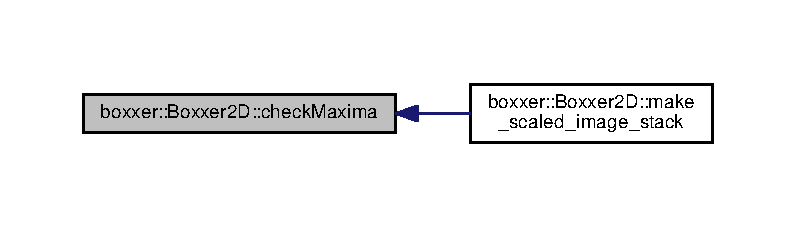
\includegraphics[width=350pt]{classboxxer_1_1Boxxer2D_a627557e88133731402ac74c03940141f_icgraph}
\end{center}
\end{figure}


\index{boxxer\+::\+Boxxer2D@{boxxer\+::\+Boxxer2D}!enumerate\+Image\+Maxima@{enumerate\+Image\+Maxima}}
\index{enumerate\+Image\+Maxima@{enumerate\+Image\+Maxima}!boxxer\+::\+Boxxer2D@{boxxer\+::\+Boxxer2D}}
\paragraph[{\texorpdfstring{enumerate\+Image\+Maxima(const Image\+Stack\+T \&im, I\+Mat\+T \&maxima, Vec\+T \&max\+\_\+vals, Idx\+T neighborhood\+\_\+size)}{enumerateImageMaxima(const ImageStackT &im, IMatT &maxima, VecT &max_vals, IdxT neighborhood_size)}}]{\setlength{\rightskip}{0pt plus 5cm}template$<$class FloatT  = float, class IdxT  = uint32\+\_\+t$>$ static IdxT {\bf boxxer\+::\+Boxxer2D}$<$ FloatT, IdxT $>$\+::enumerate\+Image\+Maxima (
\begin{DoxyParamCaption}
\item[{const {\bf Image\+StackT} \&}]{im, }
\item[{{\bf I\+MatT} \&}]{maxima, }
\item[{{\bf VecT} \&}]{max\+\_\+vals, }
\item[{IdxT}]{neighborhood\+\_\+size}
\end{DoxyParamCaption}
)\hspace{0.3cm}{\ttfamily [static]}}\hypertarget{classboxxer_1_1Boxxer2D_adc8ce4f6cb5af431aae17763d89042a5}{}\label{classboxxer_1_1Boxxer2D_adc8ce4f6cb5af431aae17763d89042a5}


Referenced by boxxer\+::\+Boxxer2\+D$<$ Float\+T, Idx\+T $>$\+::make\+\_\+scaled\+\_\+image\+\_\+stack().



Here is the caller graph for this function\+:\nopagebreak
\begin{figure}[H]
\begin{center}
\leavevmode
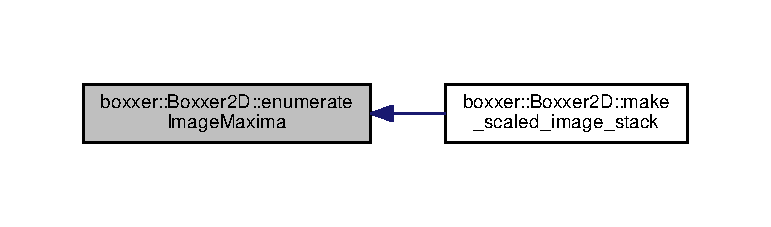
\includegraphics[width=350pt]{classboxxer_1_1Boxxer2D_adc8ce4f6cb5af431aae17763d89042a5_icgraph}
\end{center}
\end{figure}


\index{boxxer\+::\+Boxxer2D@{boxxer\+::\+Boxxer2D}!filter\+DoG@{filter\+DoG}}
\index{filter\+DoG@{filter\+DoG}!boxxer\+::\+Boxxer2D@{boxxer\+::\+Boxxer2D}}
\paragraph[{\texorpdfstring{filter\+Do\+G(const Image\+Stack\+T \&im, Image\+Stack\+T \&fim, const Vec\+T \&sigma, Float\+T sigma\+\_\+ratio)}{filterDoG(const ImageStackT &im, ImageStackT &fim, const VecT &sigma, FloatT sigma_ratio)}}]{\setlength{\rightskip}{0pt plus 5cm}template$<$class FloatT  = float, class IdxT  = uint32\+\_\+t$>$ static void {\bf boxxer\+::\+Boxxer2D}$<$ FloatT, IdxT $>$\+::filter\+DoG (
\begin{DoxyParamCaption}
\item[{const {\bf Image\+StackT} \&}]{im, }
\item[{{\bf Image\+StackT} \&}]{fim, }
\item[{const {\bf VecT} \&}]{sigma, }
\item[{FloatT}]{sigma\+\_\+ratio}
\end{DoxyParamCaption}
)\hspace{0.3cm}{\ttfamily [static]}}\hypertarget{classboxxer_1_1Boxxer2D_a42be1c0ec28f5e56b56466c23a691330}{}\label{classboxxer_1_1Boxxer2D_a42be1c0ec28f5e56b56466c23a691330}


Referenced by boxxer\+::\+Boxxer2\+D$<$ Float\+T, Idx\+T $>$\+::make\+\_\+scaled\+\_\+image\+\_\+stack().



Here is the caller graph for this function\+:\nopagebreak
\begin{figure}[H]
\begin{center}
\leavevmode
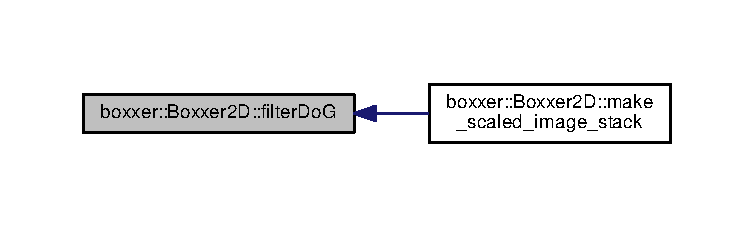
\includegraphics[width=350pt]{classboxxer_1_1Boxxer2D_a42be1c0ec28f5e56b56466c23a691330_icgraph}
\end{center}
\end{figure}


\index{boxxer\+::\+Boxxer2D@{boxxer\+::\+Boxxer2D}!filter\+Gauss@{filter\+Gauss}}
\index{filter\+Gauss@{filter\+Gauss}!boxxer\+::\+Boxxer2D@{boxxer\+::\+Boxxer2D}}
\paragraph[{\texorpdfstring{filter\+Gauss(const Image\+Stack\+T \&im, Image\+Stack\+T \&fim, const Vec\+T \&sigma)}{filterGauss(const ImageStackT &im, ImageStackT &fim, const VecT &sigma)}}]{\setlength{\rightskip}{0pt plus 5cm}template$<$class FloatT  = float, class IdxT  = uint32\+\_\+t$>$ static void {\bf boxxer\+::\+Boxxer2D}$<$ FloatT, IdxT $>$\+::filter\+Gauss (
\begin{DoxyParamCaption}
\item[{const {\bf Image\+StackT} \&}]{im, }
\item[{{\bf Image\+StackT} \&}]{fim, }
\item[{const {\bf VecT} \&}]{sigma}
\end{DoxyParamCaption}
)\hspace{0.3cm}{\ttfamily [static]}}\hypertarget{classboxxer_1_1Boxxer2D_ab02b4b192594387e705630aec04befcc}{}\label{classboxxer_1_1Boxxer2D_ab02b4b192594387e705630aec04befcc}


Referenced by boxxer\+::\+Boxxer2\+D$<$ Float\+T, Idx\+T $>$\+::make\+\_\+scaled\+\_\+image\+\_\+stack().



Here is the caller graph for this function\+:\nopagebreak
\begin{figure}[H]
\begin{center}
\leavevmode
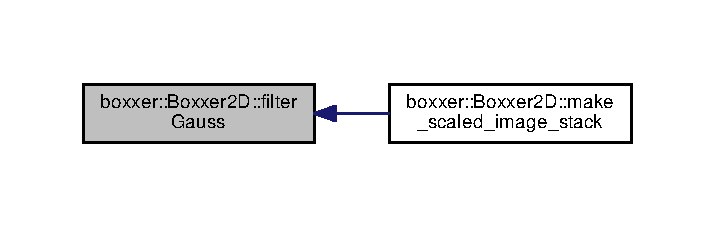
\includegraphics[width=343pt]{classboxxer_1_1Boxxer2D_ab02b4b192594387e705630aec04befcc_icgraph}
\end{center}
\end{figure}


\index{boxxer\+::\+Boxxer2D@{boxxer\+::\+Boxxer2D}!filter\+LoG@{filter\+LoG}}
\index{filter\+LoG@{filter\+LoG}!boxxer\+::\+Boxxer2D@{boxxer\+::\+Boxxer2D}}
\paragraph[{\texorpdfstring{filter\+Lo\+G(const Image\+Stack\+T \&im, Image\+Stack\+T \&fim, const Vec\+T \&sigma)}{filterLoG(const ImageStackT &im, ImageStackT &fim, const VecT &sigma)}}]{\setlength{\rightskip}{0pt plus 5cm}template$<$class FloatT  = float, class IdxT  = uint32\+\_\+t$>$ static void {\bf boxxer\+::\+Boxxer2D}$<$ FloatT, IdxT $>$\+::filter\+LoG (
\begin{DoxyParamCaption}
\item[{const {\bf Image\+StackT} \&}]{im, }
\item[{{\bf Image\+StackT} \&}]{fim, }
\item[{const {\bf VecT} \&}]{sigma}
\end{DoxyParamCaption}
)\hspace{0.3cm}{\ttfamily [static]}}\hypertarget{classboxxer_1_1Boxxer2D_a15a892fce4934b21f5c1fcba2c8cb285}{}\label{classboxxer_1_1Boxxer2D_a15a892fce4934b21f5c1fcba2c8cb285}


Referenced by boxxer\+::\+Boxxer2\+D$<$ Float\+T, Idx\+T $>$\+::make\+\_\+scaled\+\_\+image\+\_\+stack().



Here is the caller graph for this function\+:\nopagebreak
\begin{figure}[H]
\begin{center}
\leavevmode
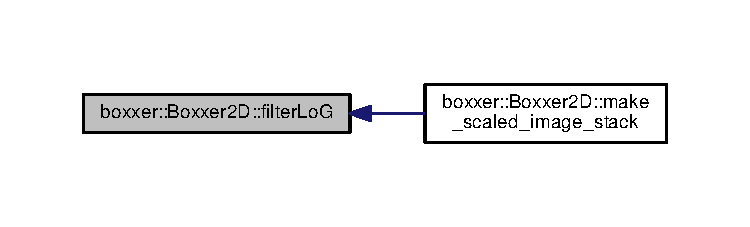
\includegraphics[width=350pt]{classboxxer_1_1Boxxer2D_a15a892fce4934b21f5c1fcba2c8cb285_icgraph}
\end{center}
\end{figure}


\index{boxxer\+::\+Boxxer2D@{boxxer\+::\+Boxxer2D}!filter\+Scaled\+DoG@{filter\+Scaled\+DoG}}
\index{filter\+Scaled\+DoG@{filter\+Scaled\+DoG}!boxxer\+::\+Boxxer2D@{boxxer\+::\+Boxxer2D}}
\paragraph[{\texorpdfstring{filter\+Scaled\+Do\+G(const Image\+Stack\+T \&im, Scaled\+Image\+Stack\+T \&fim) const }{filterScaledDoG(const ImageStackT &im, ScaledImageStackT &fim) const }}]{\setlength{\rightskip}{0pt plus 5cm}template$<$class FloatT  = float, class IdxT  = uint32\+\_\+t$>$ void {\bf boxxer\+::\+Boxxer2D}$<$ FloatT, IdxT $>$\+::filter\+Scaled\+DoG (
\begin{DoxyParamCaption}
\item[{const {\bf Image\+StackT} \&}]{im, }
\item[{{\bf Scaled\+Image\+StackT} \&}]{fim}
\end{DoxyParamCaption}
) const}\hypertarget{classboxxer_1_1Boxxer2D_a35393374b3c73f09c7a6a4a45ec82856}{}\label{classboxxer_1_1Boxxer2D_a35393374b3c73f09c7a6a4a45ec82856}
\index{boxxer\+::\+Boxxer2D@{boxxer\+::\+Boxxer2D}!filter\+Scaled\+LoG@{filter\+Scaled\+LoG}}
\index{filter\+Scaled\+LoG@{filter\+Scaled\+LoG}!boxxer\+::\+Boxxer2D@{boxxer\+::\+Boxxer2D}}
\paragraph[{\texorpdfstring{filter\+Scaled\+Lo\+G(const Image\+Stack\+T \&im, Scaled\+Image\+Stack\+T \&fim) const }{filterScaledLoG(const ImageStackT &im, ScaledImageStackT &fim) const }}]{\setlength{\rightskip}{0pt plus 5cm}template$<$class FloatT  = float, class IdxT  = uint32\+\_\+t$>$ void {\bf boxxer\+::\+Boxxer2D}$<$ FloatT, IdxT $>$\+::filter\+Scaled\+LoG (
\begin{DoxyParamCaption}
\item[{const {\bf Image\+StackT} \&}]{im, }
\item[{{\bf Scaled\+Image\+StackT} \&}]{fim}
\end{DoxyParamCaption}
) const}\hypertarget{classboxxer_1_1Boxxer2D_a3291815bf3f9a0762f542bfe636b6da4}{}\label{classboxxer_1_1Boxxer2D_a3291815bf3f9a0762f542bfe636b6da4}
\index{boxxer\+::\+Boxxer2D@{boxxer\+::\+Boxxer2D}!make\+\_\+image@{make\+\_\+image}}
\index{make\+\_\+image@{make\+\_\+image}!boxxer\+::\+Boxxer2D@{boxxer\+::\+Boxxer2D}}
\paragraph[{\texorpdfstring{make\+\_\+image() const }{make_image() const }}]{\setlength{\rightskip}{0pt plus 5cm}template$<$class FloatT  = float, class IdxT  = uint32\+\_\+t$>$ {\bf ImageT} {\bf boxxer\+::\+Boxxer2D}$<$ FloatT, IdxT $>$\+::make\+\_\+image (
\begin{DoxyParamCaption}
{}
\end{DoxyParamCaption}
) const\hspace{0.3cm}{\ttfamily [inline]}}\hypertarget{classboxxer_1_1Boxxer2D_a3a3deae8a4d6105bcf5793151278f9b7}{}\label{classboxxer_1_1Boxxer2D_a3a3deae8a4d6105bcf5793151278f9b7}


Definition at line 61 of file Boxxer2\+D.\+h.



References boxxer\+::\+Boxxer2\+D$<$ Float\+T, Idx\+T $>$\+::imsize.

\index{boxxer\+::\+Boxxer2D@{boxxer\+::\+Boxxer2D}!make\+\_\+image\+\_\+stack@{make\+\_\+image\+\_\+stack}}
\index{make\+\_\+image\+\_\+stack@{make\+\_\+image\+\_\+stack}!boxxer\+::\+Boxxer2D@{boxxer\+::\+Boxxer2D}}
\paragraph[{\texorpdfstring{make\+\_\+image\+\_\+stack(\+Idx\+T n\+T) const }{make_image_stack(IdxT nT) const }}]{\setlength{\rightskip}{0pt plus 5cm}template$<$class FloatT  = float, class IdxT  = uint32\+\_\+t$>$ {\bf Image\+StackT} {\bf boxxer\+::\+Boxxer2D}$<$ FloatT, IdxT $>$\+::make\+\_\+image\+\_\+stack (
\begin{DoxyParamCaption}
\item[{IdxT}]{nT}
\end{DoxyParamCaption}
) const\hspace{0.3cm}{\ttfamily [inline]}}\hypertarget{classboxxer_1_1Boxxer2D_aa481bbbab9b8aff1f470a5c82fb71f9b}{}\label{classboxxer_1_1Boxxer2D_aa481bbbab9b8aff1f470a5c82fb71f9b}


Definition at line 62 of file Boxxer2\+D.\+h.



References boxxer\+::\+Boxxer2\+D$<$ Float\+T, Idx\+T $>$\+::imsize.

\index{boxxer\+::\+Boxxer2D@{boxxer\+::\+Boxxer2D}!make\+\_\+scaled\+\_\+image@{make\+\_\+scaled\+\_\+image}}
\index{make\+\_\+scaled\+\_\+image@{make\+\_\+scaled\+\_\+image}!boxxer\+::\+Boxxer2D@{boxxer\+::\+Boxxer2D}}
\paragraph[{\texorpdfstring{make\+\_\+scaled\+\_\+image() const }{make_scaled_image() const }}]{\setlength{\rightskip}{0pt plus 5cm}template$<$class FloatT  = float, class IdxT  = uint32\+\_\+t$>$ {\bf Scaled\+ImageT} {\bf boxxer\+::\+Boxxer2D}$<$ FloatT, IdxT $>$\+::make\+\_\+scaled\+\_\+image (
\begin{DoxyParamCaption}
{}
\end{DoxyParamCaption}
) const\hspace{0.3cm}{\ttfamily [inline]}}\hypertarget{classboxxer_1_1Boxxer2D_a4817f3e6707a0ca9330ae6f0dbfb89da}{}\label{classboxxer_1_1Boxxer2D_a4817f3e6707a0ca9330ae6f0dbfb89da}


Definition at line 63 of file Boxxer2\+D.\+h.



References boxxer\+::\+Boxxer2\+D$<$ Float\+T, Idx\+T $>$\+::imsize.

\index{boxxer\+::\+Boxxer2D@{boxxer\+::\+Boxxer2D}!make\+\_\+scaled\+\_\+image\+\_\+stack@{make\+\_\+scaled\+\_\+image\+\_\+stack}}
\index{make\+\_\+scaled\+\_\+image\+\_\+stack@{make\+\_\+scaled\+\_\+image\+\_\+stack}!boxxer\+::\+Boxxer2D@{boxxer\+::\+Boxxer2D}}
\paragraph[{\texorpdfstring{make\+\_\+scaled\+\_\+image\+\_\+stack(\+Idx\+T n\+T) const }{make_scaled_image_stack(IdxT nT) const }}]{\setlength{\rightskip}{0pt plus 5cm}template$<$class FloatT  = float, class IdxT  = uint32\+\_\+t$>$ {\bf Scaled\+Image\+StackT} {\bf boxxer\+::\+Boxxer2D}$<$ FloatT, IdxT $>$\+::make\+\_\+scaled\+\_\+image\+\_\+stack (
\begin{DoxyParamCaption}
\item[{IdxT}]{nT}
\end{DoxyParamCaption}
) const\hspace{0.3cm}{\ttfamily [inline]}}\hypertarget{classboxxer_1_1Boxxer2D_a5c2ee267ed5ac1c61d3b7a9c935e0922}{}\label{classboxxer_1_1Boxxer2D_a5c2ee267ed5ac1c61d3b7a9c935e0922}


Definition at line 64 of file Boxxer2\+D.\+h.



References boxxer\+::\+Boxxer2\+D$<$ Float\+T, Idx\+T $>$\+::check\+Maxima(), boxxer\+::\+Boxxer2\+D$<$ Float\+T, Idx\+T $>$\+::enumerate\+Image\+Maxima(), boxxer\+::\+Boxxer2\+D$<$ Float\+T, Idx\+T $>$\+::filter\+Do\+G(), boxxer\+::\+Boxxer2\+D$<$ Float\+T, Idx\+T $>$\+::filter\+Gauss(), boxxer\+::\+Boxxer2\+D$<$ Float\+T, Idx\+T $>$\+::filter\+Lo\+G(), and boxxer\+::\+Boxxer2\+D$<$ Float\+T, Idx\+T $>$\+::imsize.



Here is the call graph for this function\+:\nopagebreak
\begin{figure}[H]
\begin{center}
\leavevmode
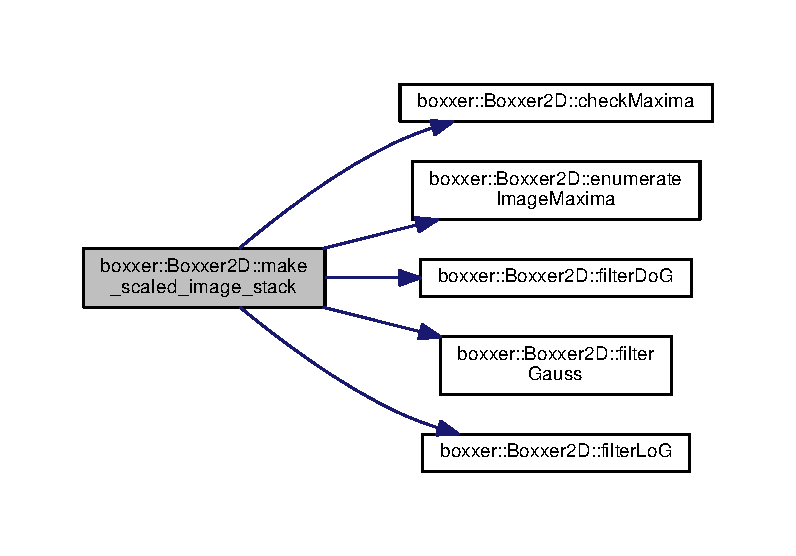
\includegraphics[width=350pt]{classboxxer_1_1Boxxer2D_a5c2ee267ed5ac1c61d3b7a9c935e0922_cgraph}
\end{center}
\end{figure}


\index{boxxer\+::\+Boxxer2D@{boxxer\+::\+Boxxer2D}!scale\+Space\+Do\+G\+Maxima@{scale\+Space\+Do\+G\+Maxima}}
\index{scale\+Space\+Do\+G\+Maxima@{scale\+Space\+Do\+G\+Maxima}!boxxer\+::\+Boxxer2D@{boxxer\+::\+Boxxer2D}}
\paragraph[{\texorpdfstring{scale\+Space\+Do\+G\+Maxima(const Image\+Stack\+T \&im, I\+Mat\+T \&maxima, Vec\+T \&max\+\_\+vals, Idx\+T neighborhood\+\_\+size, Idx\+T scale\+\_\+neighborhood\+\_\+size) const }{scaleSpaceDoGMaxima(const ImageStackT &im, IMatT &maxima, VecT &max_vals, IdxT neighborhood_size, IdxT scale_neighborhood_size) const }}]{\setlength{\rightskip}{0pt plus 5cm}template$<$class FloatT  = float, class IdxT  = uint32\+\_\+t$>$ IdxT {\bf boxxer\+::\+Boxxer2D}$<$ FloatT, IdxT $>$\+::scale\+Space\+Do\+G\+Maxima (
\begin{DoxyParamCaption}
\item[{const {\bf Image\+StackT} \&}]{im, }
\item[{{\bf I\+MatT} \&}]{maxima, }
\item[{{\bf VecT} \&}]{max\+\_\+vals, }
\item[{IdxT}]{neighborhood\+\_\+size, }
\item[{IdxT}]{scale\+\_\+neighborhood\+\_\+size}
\end{DoxyParamCaption}
) const}\hypertarget{classboxxer_1_1Boxxer2D_ad3d93a33dcef252f4f0be57a27535f6e}{}\label{classboxxer_1_1Boxxer2D_ad3d93a33dcef252f4f0be57a27535f6e}
\index{boxxer\+::\+Boxxer2D@{boxxer\+::\+Boxxer2D}!scale\+Space\+Lo\+G\+Maxima@{scale\+Space\+Lo\+G\+Maxima}}
\index{scale\+Space\+Lo\+G\+Maxima@{scale\+Space\+Lo\+G\+Maxima}!boxxer\+::\+Boxxer2D@{boxxer\+::\+Boxxer2D}}
\paragraph[{\texorpdfstring{scale\+Space\+Lo\+G\+Maxima(const Image\+Stack\+T \&im, I\+Mat\+T \&maxima, Vec\+T \&max\+\_\+vals, Idx\+T neighborhood\+\_\+size, Idx\+T scale\+\_\+neighborhood\+\_\+size) const }{scaleSpaceLoGMaxima(const ImageStackT &im, IMatT &maxima, VecT &max_vals, IdxT neighborhood_size, IdxT scale_neighborhood_size) const }}]{\setlength{\rightskip}{0pt plus 5cm}template$<$class FloatT  = float, class IdxT  = uint32\+\_\+t$>$ IdxT {\bf boxxer\+::\+Boxxer2D}$<$ FloatT, IdxT $>$\+::scale\+Space\+Lo\+G\+Maxima (
\begin{DoxyParamCaption}
\item[{const {\bf Image\+StackT} \&}]{im, }
\item[{{\bf I\+MatT} \&}]{maxima, }
\item[{{\bf VecT} \&}]{max\+\_\+vals, }
\item[{IdxT}]{neighborhood\+\_\+size, }
\item[{IdxT}]{scale\+\_\+neighborhood\+\_\+size}
\end{DoxyParamCaption}
) const}\hypertarget{classboxxer_1_1Boxxer2D_ad5dffcdf4797f49541b9c44c9551987a}{}\label{classboxxer_1_1Boxxer2D_ad5dffcdf4797f49541b9c44c9551987a}
\index{boxxer\+::\+Boxxer2D@{boxxer\+::\+Boxxer2D}!set\+Do\+G\+Sigma\+Ratio@{set\+Do\+G\+Sigma\+Ratio}}
\index{set\+Do\+G\+Sigma\+Ratio@{set\+Do\+G\+Sigma\+Ratio}!boxxer\+::\+Boxxer2D@{boxxer\+::\+Boxxer2D}}
\paragraph[{\texorpdfstring{set\+Do\+G\+Sigma\+Ratio(\+Float\+T sigma\+\_\+ratio)}{setDoGSigmaRatio(FloatT sigma_ratio)}}]{\setlength{\rightskip}{0pt plus 5cm}template$<$class FloatT  = float, class IdxT  = uint32\+\_\+t$>$ void {\bf boxxer\+::\+Boxxer2D}$<$ FloatT, IdxT $>$\+::set\+Do\+G\+Sigma\+Ratio (
\begin{DoxyParamCaption}
\item[{FloatT}]{sigma\+\_\+ratio}
\end{DoxyParamCaption}
)}\hypertarget{classboxxer_1_1Boxxer2D_a9fcfdebe9f2896232c50b482005db219}{}\label{classboxxer_1_1Boxxer2D_a9fcfdebe9f2896232c50b482005db219}


\subsubsection{Member Data Documentation}
\index{boxxer\+::\+Boxxer2D@{boxxer\+::\+Boxxer2D}!Default\+Sigma\+Ratio@{Default\+Sigma\+Ratio}}
\index{Default\+Sigma\+Ratio@{Default\+Sigma\+Ratio}!boxxer\+::\+Boxxer2D@{boxxer\+::\+Boxxer2D}}
\paragraph[{\texorpdfstring{Default\+Sigma\+Ratio}{DefaultSigmaRatio}}]{\setlength{\rightskip}{0pt plus 5cm}template$<$class FloatT  = float, class IdxT  = uint32\+\_\+t$>$ const FloatT {\bf boxxer\+::\+Boxxer2D}$<$ FloatT, IdxT $>$\+::Default\+Sigma\+Ratio\hspace{0.3cm}{\ttfamily [static]}}\hypertarget{classboxxer_1_1Boxxer2D_a2175ae26a8a47e6bc57a6fb89cc9e177}{}\label{classboxxer_1_1Boxxer2D_a2175ae26a8a47e6bc57a6fb89cc9e177}


Definition at line 45 of file Boxxer2\+D.\+h.

\index{boxxer\+::\+Boxxer2D@{boxxer\+::\+Boxxer2D}!dim@{dim}}
\index{dim@{dim}!boxxer\+::\+Boxxer2D@{boxxer\+::\+Boxxer2D}}
\paragraph[{\texorpdfstring{dim}{dim}}]{\setlength{\rightskip}{0pt plus 5cm}template$<$class FloatT  = float, class IdxT  = uint32\+\_\+t$>$ const IdxT {\bf boxxer\+::\+Boxxer2D}$<$ FloatT, IdxT $>$\+::dim\hspace{0.3cm}{\ttfamily [static]}}\hypertarget{classboxxer_1_1Boxxer2D_a66f41631af87252601a33480c0433eea}{}\label{classboxxer_1_1Boxxer2D_a66f41631af87252601a33480c0433eea}


Definition at line 46 of file Boxxer2\+D.\+h.

\index{boxxer\+::\+Boxxer2D@{boxxer\+::\+Boxxer2D}!imsize@{imsize}}
\index{imsize@{imsize}!boxxer\+::\+Boxxer2D@{boxxer\+::\+Boxxer2D}}
\paragraph[{\texorpdfstring{imsize}{imsize}}]{\setlength{\rightskip}{0pt plus 5cm}template$<$class FloatT  = float, class IdxT  = uint32\+\_\+t$>$ {\bf I\+VecT} {\bf boxxer\+::\+Boxxer2D}$<$ FloatT, IdxT $>$\+::imsize}\hypertarget{classboxxer_1_1Boxxer2D_a6f76692e32f0c907d48a72a801a62b9a}{}\label{classboxxer_1_1Boxxer2D_a6f76692e32f0c907d48a72a801a62b9a}


Definition at line 49 of file Boxxer2\+D.\+h.



Referenced by boxxer\+::\+Boxxer2\+D$<$ Float\+T, Idx\+T $>$\+::make\+\_\+image(), boxxer\+::\+Boxxer2\+D$<$ Float\+T, Idx\+T $>$\+::make\+\_\+image\+\_\+stack(), boxxer\+::\+Boxxer2\+D$<$ Float\+T, Idx\+T $>$\+::make\+\_\+scaled\+\_\+image(), and boxxer\+::\+Boxxer2\+D$<$ Float\+T, Idx\+T $>$\+::make\+\_\+scaled\+\_\+image\+\_\+stack().

\index{boxxer\+::\+Boxxer2D@{boxxer\+::\+Boxxer2D}!n\+Scales@{n\+Scales}}
\index{n\+Scales@{n\+Scales}!boxxer\+::\+Boxxer2D@{boxxer\+::\+Boxxer2D}}
\paragraph[{\texorpdfstring{n\+Scales}{nScales}}]{\setlength{\rightskip}{0pt plus 5cm}template$<$class FloatT  = float, class IdxT  = uint32\+\_\+t$>$ IdxT {\bf boxxer\+::\+Boxxer2D}$<$ FloatT, IdxT $>$\+::n\+Scales}\hypertarget{classboxxer_1_1Boxxer2D_a7577d773fec8de75968ef12fe2c1c59b}{}\label{classboxxer_1_1Boxxer2D_a7577d773fec8de75968ef12fe2c1c59b}


Definition at line 48 of file Boxxer2\+D.\+h.

\index{boxxer\+::\+Boxxer2D@{boxxer\+::\+Boxxer2D}!sigma@{sigma}}
\index{sigma@{sigma}!boxxer\+::\+Boxxer2D@{boxxer\+::\+Boxxer2D}}
\paragraph[{\texorpdfstring{sigma}{sigma}}]{\setlength{\rightskip}{0pt plus 5cm}template$<$class FloatT  = float, class IdxT  = uint32\+\_\+t$>$ {\bf MatT} {\bf boxxer\+::\+Boxxer2D}$<$ FloatT, IdxT $>$\+::sigma}\hypertarget{classboxxer_1_1Boxxer2D_a925fe4151cca3a34cba36f1a10b8e382}{}\label{classboxxer_1_1Boxxer2D_a925fe4151cca3a34cba36f1a10b8e382}


Definition at line 50 of file Boxxer2\+D.\+h.

\index{boxxer\+::\+Boxxer2D@{boxxer\+::\+Boxxer2D}!sigma\+\_\+ratio@{sigma\+\_\+ratio}}
\index{sigma\+\_\+ratio@{sigma\+\_\+ratio}!boxxer\+::\+Boxxer2D@{boxxer\+::\+Boxxer2D}}
\paragraph[{\texorpdfstring{sigma\+\_\+ratio}{sigma_ratio}}]{\setlength{\rightskip}{0pt plus 5cm}template$<$class FloatT  = float, class IdxT  = uint32\+\_\+t$>$ FloatT {\bf boxxer\+::\+Boxxer2D}$<$ FloatT, IdxT $>$\+::sigma\+\_\+ratio}\hypertarget{classboxxer_1_1Boxxer2D_a0fffedee4a39644c5c48fba99e297111}{}\label{classboxxer_1_1Boxxer2D_a0fffedee4a39644c5c48fba99e297111}


Definition at line 51 of file Boxxer2\+D.\+h.



The documentation for this class was generated from the following file\+:\begin{DoxyCompactItemize}
\item 
\hyperlink{Boxxer2D_8h}{Boxxer2\+D.\+h}\end{DoxyCompactItemize}

\hypertarget{classboxxer_1_1Boxxer3D}{}\subsection{boxxer\+:\+:Boxxer3D$<$ FloatT, IdxT $>$ Class Template Reference}
\label{classboxxer_1_1Boxxer3D}\index{boxxer\+::\+Boxxer3\+D$<$ Float\+T, Idx\+T $>$@{boxxer\+::\+Boxxer3\+D$<$ Float\+T, Idx\+T $>$}}


{\ttfamily \#include $<$/home/travis/build/markjolah/\+Boxxer/include/\+Boxxer/\+Boxxer3\+D.\+h$>$}

\subsubsection*{Public Types}
\begin{DoxyCompactItemize}
\item 
using \hyperlink{classboxxer_1_1Boxxer3D_a62a7f35aa283e2a833d13edaa228bca2}{I\+VecT} = arma\+::\+Col$<$ IdxT $>$
\item 
using \hyperlink{classboxxer_1_1Boxxer3D_a9b8cb89e1f1fbf091e5443876ca9a200}{I\+MatT} = arma\+::\+Mat$<$ IdxT $>$
\item 
using \hyperlink{classboxxer_1_1Boxxer3D_a74e56a85bc18204a802bbf2a76eea61c}{VecT} = arma\+::\+Col$<$ FloatT $>$
\item 
using \hyperlink{classboxxer_1_1Boxxer3D_ae155080a591506ca84d3d70f1cde337d}{MatT} = arma\+::\+Mat$<$ FloatT $>$
\item 
using \hyperlink{classboxxer_1_1Boxxer3D_a8990923b1207fc8ae066de124ab75053}{ImageT} = arma\+::\+Cube$<$ FloatT $>$
\item 
using \hyperlink{classboxxer_1_1Boxxer3D_aa17e25866089479e9b40ea01dfad8a88}{Image\+StackT} = hypercube\+::\+Hypercube$<$ FloatT $>$
\item 
using \hyperlink{classboxxer_1_1Boxxer3D_aefd3895d7a0790a08de4714ee7a59d97}{Scaled\+ImageT} = hypercube\+::\+Hypercube$<$ FloatT $>$
\end{DoxyCompactItemize}
\subsubsection*{Public Member Functions}
\begin{DoxyCompactItemize}
\item 
\hyperlink{classboxxer_1_1Boxxer3D_ac010173e25bea7fcfbf7a532ec00de1f}{Boxxer3D} (const \hyperlink{classboxxer_1_1Boxxer3D_a62a7f35aa283e2a833d13edaa228bca2}{I\+VecT} \&size, const \hyperlink{classboxxer_1_1Boxxer3D_ae155080a591506ca84d3d70f1cde337d}{MatT} \&\hyperlink{classboxxer_1_1Boxxer3D_a5df6b670e57ee7b6c2396650f6caba86}{sigma})
\item 
void \hyperlink{classboxxer_1_1Boxxer3D_a22933f928d48cfa58dbada555d8a1d1e}{set\+Do\+G\+Sigma\+Ratio} (FloatT \hyperlink{classboxxer_1_1Boxxer3D_a63a9a0d9c56c11f34c7f2c80e0556335}{sigma\+\_\+ratio})
\item 
void \hyperlink{classboxxer_1_1Boxxer3D_a54ce058d4f00b44b40808cdc964ea7f5}{filter\+Scaled\+LoG} (const \hyperlink{classboxxer_1_1Boxxer3D_a8990923b1207fc8ae066de124ab75053}{ImageT} \&im, \hyperlink{classboxxer_1_1Boxxer3D_aefd3895d7a0790a08de4714ee7a59d97}{Scaled\+ImageT} \&fim)
\item 
void \hyperlink{classboxxer_1_1Boxxer3D_ae1e5a4f23ea5909e10e0545e56e334df}{filter\+Scaled\+DoG} (const \hyperlink{classboxxer_1_1Boxxer3D_a8990923b1207fc8ae066de124ab75053}{ImageT} \&im, \hyperlink{classboxxer_1_1Boxxer3D_aefd3895d7a0790a08de4714ee7a59d97}{Scaled\+ImageT} \&fim)
\item 
IdxT \hyperlink{classboxxer_1_1Boxxer3D_aa3a28765766e21dc7b994da8c056fe47}{scale\+Space\+Lo\+G\+Maxima} (const \hyperlink{classboxxer_1_1Boxxer3D_aa17e25866089479e9b40ea01dfad8a88}{Image\+StackT} \&im, \hyperlink{classboxxer_1_1Boxxer3D_a9b8cb89e1f1fbf091e5443876ca9a200}{I\+MatT} \&maxima, \hyperlink{classboxxer_1_1Boxxer3D_a74e56a85bc18204a802bbf2a76eea61c}{VecT} \&max\+\_\+vals, IdxT neighborhood\+\_\+size, IdxT scale\+\_\+neighborhood\+\_\+size)
\item 
IdxT \hyperlink{classboxxer_1_1Boxxer3D_a66040edbfb27cdc2d73be9789b7ca676}{scale\+Space\+Do\+G\+Maxima} (const \hyperlink{classboxxer_1_1Boxxer3D_aa17e25866089479e9b40ea01dfad8a88}{Image\+StackT} \&im, \hyperlink{classboxxer_1_1Boxxer3D_a9b8cb89e1f1fbf091e5443876ca9a200}{I\+MatT} \&maxima, \hyperlink{classboxxer_1_1Boxxer3D_a74e56a85bc18204a802bbf2a76eea61c}{VecT} \&max\+\_\+vals, IdxT neighborhood\+\_\+size, IdxT scale\+\_\+neighborhood\+\_\+size)
\item 
\hyperlink{classboxxer_1_1Boxxer3D_a8990923b1207fc8ae066de124ab75053}{ImageT} \hyperlink{classboxxer_1_1Boxxer3D_a8e86e20a67d0275319436b6d76f8c765}{make\+\_\+image} () const 
\item 
\hyperlink{classboxxer_1_1Boxxer3D_aa17e25866089479e9b40ea01dfad8a88}{Image\+StackT} \hyperlink{classboxxer_1_1Boxxer3D_a25c358eb9570f8a32d892e89b4b02e90}{make\+\_\+image\+\_\+stack} (IdxT nT) const 
\item 
\hyperlink{classboxxer_1_1Boxxer3D_aefd3895d7a0790a08de4714ee7a59d97}{Scaled\+ImageT} \hyperlink{classboxxer_1_1Boxxer3D_a3bc9609e6bdb4a6aac10aea313b70b12}{make\+\_\+scaled\+\_\+image} () const 
\end{DoxyCompactItemize}
\subsubsection*{Static Public Member Functions}
\begin{DoxyCompactItemize}
\item 
static void \hyperlink{classboxxer_1_1Boxxer3D_ad242333de1472fea719db9958dfe6f46}{filter\+LoG} (const \hyperlink{classboxxer_1_1Boxxer3D_aa17e25866089479e9b40ea01dfad8a88}{Image\+StackT} \&im, \hyperlink{classboxxer_1_1Boxxer3D_aa17e25866089479e9b40ea01dfad8a88}{Image\+StackT} \&fim, const \hyperlink{classboxxer_1_1Boxxer3D_a74e56a85bc18204a802bbf2a76eea61c}{VecT} \&\hyperlink{classboxxer_1_1Boxxer3D_a5df6b670e57ee7b6c2396650f6caba86}{sigma})
\item 
static void \hyperlink{classboxxer_1_1Boxxer3D_a523dff6ee90ba9f6e6bb0e8e4258a905}{filter\+DoG} (const \hyperlink{classboxxer_1_1Boxxer3D_aa17e25866089479e9b40ea01dfad8a88}{Image\+StackT} \&im, \hyperlink{classboxxer_1_1Boxxer3D_aa17e25866089479e9b40ea01dfad8a88}{Image\+StackT} \&fim, const \hyperlink{classboxxer_1_1Boxxer3D_a74e56a85bc18204a802bbf2a76eea61c}{VecT} \&\hyperlink{classboxxer_1_1Boxxer3D_a5df6b670e57ee7b6c2396650f6caba86}{sigma}, FloatT \hyperlink{classboxxer_1_1Boxxer3D_a63a9a0d9c56c11f34c7f2c80e0556335}{sigma\+\_\+ratio})
\item 
static void \hyperlink{classboxxer_1_1Boxxer3D_a210c289db79c6db6596df92d77052f47}{filter\+Gauss} (const \hyperlink{classboxxer_1_1Boxxer3D_aa17e25866089479e9b40ea01dfad8a88}{Image\+StackT} \&im, \hyperlink{classboxxer_1_1Boxxer3D_aa17e25866089479e9b40ea01dfad8a88}{Image\+StackT} \&fim, const \hyperlink{classboxxer_1_1Boxxer3D_a74e56a85bc18204a802bbf2a76eea61c}{VecT} \&\hyperlink{classboxxer_1_1Boxxer3D_a5df6b670e57ee7b6c2396650f6caba86}{sigma})
\item 
static void \hyperlink{classboxxer_1_1Boxxer3D_a44cf5445f8991f735207651fcb6d5962}{check\+Maxima} (const \hyperlink{classboxxer_1_1Boxxer3D_aa17e25866089479e9b40ea01dfad8a88}{Image\+StackT} \&im, \hyperlink{classboxxer_1_1Boxxer3D_a9b8cb89e1f1fbf091e5443876ca9a200}{I\+MatT} \&maxima, \hyperlink{classboxxer_1_1Boxxer3D_a74e56a85bc18204a802bbf2a76eea61c}{VecT} \&max\+\_\+vals)
\item 
static IdxT \hyperlink{classboxxer_1_1Boxxer3D_a2fbe5c1f5d3b705ddcca7d13a92f9283}{enumerate\+Image\+Maxima} (const \hyperlink{classboxxer_1_1Boxxer3D_aa17e25866089479e9b40ea01dfad8a88}{Image\+StackT} \&im, \hyperlink{classboxxer_1_1Boxxer3D_a9b8cb89e1f1fbf091e5443876ca9a200}{I\+MatT} \&maxima, \hyperlink{classboxxer_1_1Boxxer3D_a74e56a85bc18204a802bbf2a76eea61c}{VecT} \&max\+\_\+vals, IdxT neighborhood\+\_\+size)
\end{DoxyCompactItemize}
\subsubsection*{Public Attributes}
\begin{DoxyCompactItemize}
\item 
IdxT \hyperlink{classboxxer_1_1Boxxer3D_a344ef289cd330d4353c4605f2c2e2bbc}{n\+Scales}
\item 
\hyperlink{classboxxer_1_1Boxxer3D_a62a7f35aa283e2a833d13edaa228bca2}{I\+VecT} \hyperlink{classboxxer_1_1Boxxer3D_a236f3f4ada01376204e59f9f68d5fde6}{imsize}
\item 
\hyperlink{classboxxer_1_1Boxxer3D_ae155080a591506ca84d3d70f1cde337d}{MatT} \hyperlink{classboxxer_1_1Boxxer3D_a5df6b670e57ee7b6c2396650f6caba86}{sigma}
\item 
FloatT \hyperlink{classboxxer_1_1Boxxer3D_a63a9a0d9c56c11f34c7f2c80e0556335}{sigma\+\_\+ratio}
\end{DoxyCompactItemize}
\subsubsection*{Static Public Attributes}
\begin{DoxyCompactItemize}
\item 
static const FloatT \hyperlink{classboxxer_1_1Boxxer3D_a8a489401adebfc449a1e9390dcdfbbf4}{Default\+Sigma\+Ratio}
\item 
static const IdxT \hyperlink{classboxxer_1_1Boxxer3D_a8ae92f1badc81d59b178c12fb339e251}{dim}
\end{DoxyCompactItemize}


\subsubsection{Detailed Description}
\subsubsection*{template$<$class FloatT = float, class IdxT = uint32\+\_\+t$>$\\*
class boxxer\+::\+Boxxer3\+D$<$ Float\+T, Idx\+T $>$}

A box finding algorithm for 3D hyper-\/spectral microscopy data.

Estimates the center coordinates of Gaussian blobs with anisotropic sigmas.

All image data manipulated is stored as column-\/major FloatT arrays with dimension ordering \mbox{[}L Y X T\mbox{]}.

The \hyperlink{classboxxer_1_1Boxxer3D}{Boxxer3D} class makes uses of lower level class which are agnostic about the data source being hyperspectral, they don\textquotesingle{}t care what the coordinate dimensions represent scientifically, but this class is associated with the Matlab \hyperlink{classboxxer_1_1Boxxer3D}{Boxxer3D} class and so maintains the knowledge that the actual coordinates are \mbox{[}L Y X T\mbox{]}. 

Definition at line 27 of file Boxxer3\+D.\+h.



\subsubsection{Member Typedef Documentation}
\index{boxxer\+::\+Boxxer3D@{boxxer\+::\+Boxxer3D}!Image\+StackT@{Image\+StackT}}
\index{Image\+StackT@{Image\+StackT}!boxxer\+::\+Boxxer3D@{boxxer\+::\+Boxxer3D}}
\paragraph[{\texorpdfstring{Image\+StackT}{ImageStackT}}]{\setlength{\rightskip}{0pt plus 5cm}template$<$class FloatT  = float, class IdxT  = uint32\+\_\+t$>$ using {\bf boxxer\+::\+Boxxer3D}$<$ FloatT, IdxT $>$\+::{\bf Image\+StackT} =  hypercube\+::\+Hypercube$<$FloatT$>$}\hypertarget{classboxxer_1_1Boxxer3D_aa17e25866089479e9b40ea01dfad8a88}{}\label{classboxxer_1_1Boxxer3D_aa17e25866089479e9b40ea01dfad8a88}


Definition at line 35 of file Boxxer3\+D.\+h.

\index{boxxer\+::\+Boxxer3D@{boxxer\+::\+Boxxer3D}!ImageT@{ImageT}}
\index{ImageT@{ImageT}!boxxer\+::\+Boxxer3D@{boxxer\+::\+Boxxer3D}}
\paragraph[{\texorpdfstring{ImageT}{ImageT}}]{\setlength{\rightskip}{0pt plus 5cm}template$<$class FloatT  = float, class IdxT  = uint32\+\_\+t$>$ using {\bf boxxer\+::\+Boxxer3D}$<$ FloatT, IdxT $>$\+::{\bf ImageT} =  arma\+::\+Cube$<$FloatT$>$}\hypertarget{classboxxer_1_1Boxxer3D_a8990923b1207fc8ae066de124ab75053}{}\label{classboxxer_1_1Boxxer3D_a8990923b1207fc8ae066de124ab75053}


Definition at line 34 of file Boxxer3\+D.\+h.

\index{boxxer\+::\+Boxxer3D@{boxxer\+::\+Boxxer3D}!I\+MatT@{I\+MatT}}
\index{I\+MatT@{I\+MatT}!boxxer\+::\+Boxxer3D@{boxxer\+::\+Boxxer3D}}
\paragraph[{\texorpdfstring{I\+MatT}{IMatT}}]{\setlength{\rightskip}{0pt plus 5cm}template$<$class FloatT  = float, class IdxT  = uint32\+\_\+t$>$ using {\bf boxxer\+::\+Boxxer3D}$<$ FloatT, IdxT $>$\+::{\bf I\+MatT} =  arma\+::\+Mat$<$IdxT$>$}\hypertarget{classboxxer_1_1Boxxer3D_a9b8cb89e1f1fbf091e5443876ca9a200}{}\label{classboxxer_1_1Boxxer3D_a9b8cb89e1f1fbf091e5443876ca9a200}


Definition at line 31 of file Boxxer3\+D.\+h.

\index{boxxer\+::\+Boxxer3D@{boxxer\+::\+Boxxer3D}!I\+VecT@{I\+VecT}}
\index{I\+VecT@{I\+VecT}!boxxer\+::\+Boxxer3D@{boxxer\+::\+Boxxer3D}}
\paragraph[{\texorpdfstring{I\+VecT}{IVecT}}]{\setlength{\rightskip}{0pt plus 5cm}template$<$class FloatT  = float, class IdxT  = uint32\+\_\+t$>$ using {\bf boxxer\+::\+Boxxer3D}$<$ FloatT, IdxT $>$\+::{\bf I\+VecT} =  arma\+::\+Col$<$IdxT$>$}\hypertarget{classboxxer_1_1Boxxer3D_a62a7f35aa283e2a833d13edaa228bca2}{}\label{classboxxer_1_1Boxxer3D_a62a7f35aa283e2a833d13edaa228bca2}


Definition at line 30 of file Boxxer3\+D.\+h.

\index{boxxer\+::\+Boxxer3D@{boxxer\+::\+Boxxer3D}!MatT@{MatT}}
\index{MatT@{MatT}!boxxer\+::\+Boxxer3D@{boxxer\+::\+Boxxer3D}}
\paragraph[{\texorpdfstring{MatT}{MatT}}]{\setlength{\rightskip}{0pt plus 5cm}template$<$class FloatT  = float, class IdxT  = uint32\+\_\+t$>$ using {\bf boxxer\+::\+Boxxer3D}$<$ FloatT, IdxT $>$\+::{\bf MatT} =  arma\+::\+Mat$<$FloatT$>$}\hypertarget{classboxxer_1_1Boxxer3D_ae155080a591506ca84d3d70f1cde337d}{}\label{classboxxer_1_1Boxxer3D_ae155080a591506ca84d3d70f1cde337d}


Definition at line 33 of file Boxxer3\+D.\+h.

\index{boxxer\+::\+Boxxer3D@{boxxer\+::\+Boxxer3D}!Scaled\+ImageT@{Scaled\+ImageT}}
\index{Scaled\+ImageT@{Scaled\+ImageT}!boxxer\+::\+Boxxer3D@{boxxer\+::\+Boxxer3D}}
\paragraph[{\texorpdfstring{Scaled\+ImageT}{ScaledImageT}}]{\setlength{\rightskip}{0pt plus 5cm}template$<$class FloatT  = float, class IdxT  = uint32\+\_\+t$>$ using {\bf boxxer\+::\+Boxxer3D}$<$ FloatT, IdxT $>$\+::{\bf Scaled\+ImageT} =  hypercube\+::\+Hypercube$<$FloatT$>$}\hypertarget{classboxxer_1_1Boxxer3D_aefd3895d7a0790a08de4714ee7a59d97}{}\label{classboxxer_1_1Boxxer3D_aefd3895d7a0790a08de4714ee7a59d97}


Definition at line 36 of file Boxxer3\+D.\+h.

\index{boxxer\+::\+Boxxer3D@{boxxer\+::\+Boxxer3D}!VecT@{VecT}}
\index{VecT@{VecT}!boxxer\+::\+Boxxer3D@{boxxer\+::\+Boxxer3D}}
\paragraph[{\texorpdfstring{VecT}{VecT}}]{\setlength{\rightskip}{0pt plus 5cm}template$<$class FloatT  = float, class IdxT  = uint32\+\_\+t$>$ using {\bf boxxer\+::\+Boxxer3D}$<$ FloatT, IdxT $>$\+::{\bf VecT} =  arma\+::\+Col$<$FloatT$>$}\hypertarget{classboxxer_1_1Boxxer3D_a74e56a85bc18204a802bbf2a76eea61c}{}\label{classboxxer_1_1Boxxer3D_a74e56a85bc18204a802bbf2a76eea61c}


Definition at line 32 of file Boxxer3\+D.\+h.



\subsubsection{Constructor \& Destructor Documentation}
\index{boxxer\+::\+Boxxer3D@{boxxer\+::\+Boxxer3D}!Boxxer3D@{Boxxer3D}}
\index{Boxxer3D@{Boxxer3D}!boxxer\+::\+Boxxer3D@{boxxer\+::\+Boxxer3D}}
\paragraph[{\texorpdfstring{Boxxer3\+D(const I\+Vec\+T \&size, const Mat\+T \&sigma)}{Boxxer3D(const IVecT &size, const MatT &sigma)}}]{\setlength{\rightskip}{0pt plus 5cm}template$<$class FloatT  = float, class IdxT  = uint32\+\_\+t$>$ {\bf boxxer\+::\+Boxxer3D}$<$ FloatT, IdxT $>$\+::{\bf Boxxer3D} (
\begin{DoxyParamCaption}
\item[{const {\bf I\+VecT} \&}]{size, }
\item[{const {\bf MatT} \&}]{sigma}
\end{DoxyParamCaption}
)}\hypertarget{classboxxer_1_1Boxxer3D_ac010173e25bea7fcfbf7a532ec00de1f}{}\label{classboxxer_1_1Boxxer3D_ac010173e25bea7fcfbf7a532ec00de1f}


\subsubsection{Member Function Documentation}
\index{boxxer\+::\+Boxxer3D@{boxxer\+::\+Boxxer3D}!check\+Maxima@{check\+Maxima}}
\index{check\+Maxima@{check\+Maxima}!boxxer\+::\+Boxxer3D@{boxxer\+::\+Boxxer3D}}
\paragraph[{\texorpdfstring{check\+Maxima(const Image\+Stack\+T \&im, I\+Mat\+T \&maxima, Vec\+T \&max\+\_\+vals)}{checkMaxima(const ImageStackT &im, IMatT &maxima, VecT &max_vals)}}]{\setlength{\rightskip}{0pt plus 5cm}template$<$class FloatT  = float, class IdxT  = uint32\+\_\+t$>$ static void {\bf boxxer\+::\+Boxxer3D}$<$ FloatT, IdxT $>$\+::check\+Maxima (
\begin{DoxyParamCaption}
\item[{const {\bf Image\+StackT} \&}]{im, }
\item[{{\bf I\+MatT} \&}]{maxima, }
\item[{{\bf VecT} \&}]{max\+\_\+vals}
\end{DoxyParamCaption}
)\hspace{0.3cm}{\ttfamily [static]}}\hypertarget{classboxxer_1_1Boxxer3D_a44cf5445f8991f735207651fcb6d5962}{}\label{classboxxer_1_1Boxxer3D_a44cf5445f8991f735207651fcb6d5962}


Referenced by boxxer\+::\+Boxxer3\+D$<$ Float\+T, Idx\+T $>$\+::make\+\_\+scaled\+\_\+image().



Here is the caller graph for this function\+:\nopagebreak
\begin{figure}[H]
\begin{center}
\leavevmode
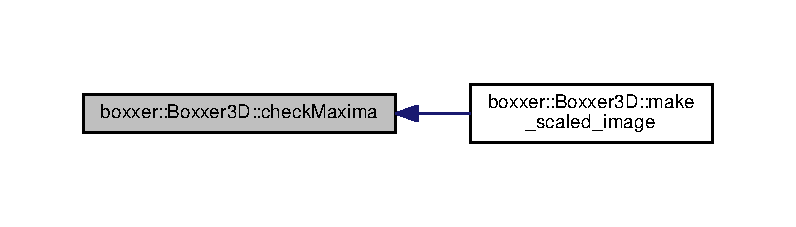
\includegraphics[width=350pt]{classboxxer_1_1Boxxer3D_a44cf5445f8991f735207651fcb6d5962_icgraph}
\end{center}
\end{figure}


\index{boxxer\+::\+Boxxer3D@{boxxer\+::\+Boxxer3D}!enumerate\+Image\+Maxima@{enumerate\+Image\+Maxima}}
\index{enumerate\+Image\+Maxima@{enumerate\+Image\+Maxima}!boxxer\+::\+Boxxer3D@{boxxer\+::\+Boxxer3D}}
\paragraph[{\texorpdfstring{enumerate\+Image\+Maxima(const Image\+Stack\+T \&im, I\+Mat\+T \&maxima, Vec\+T \&max\+\_\+vals, Idx\+T neighborhood\+\_\+size)}{enumerateImageMaxima(const ImageStackT &im, IMatT &maxima, VecT &max_vals, IdxT neighborhood_size)}}]{\setlength{\rightskip}{0pt plus 5cm}template$<$class FloatT  = float, class IdxT  = uint32\+\_\+t$>$ static IdxT {\bf boxxer\+::\+Boxxer3D}$<$ FloatT, IdxT $>$\+::enumerate\+Image\+Maxima (
\begin{DoxyParamCaption}
\item[{const {\bf Image\+StackT} \&}]{im, }
\item[{{\bf I\+MatT} \&}]{maxima, }
\item[{{\bf VecT} \&}]{max\+\_\+vals, }
\item[{IdxT}]{neighborhood\+\_\+size}
\end{DoxyParamCaption}
)\hspace{0.3cm}{\ttfamily [static]}}\hypertarget{classboxxer_1_1Boxxer3D_a2fbe5c1f5d3b705ddcca7d13a92f9283}{}\label{classboxxer_1_1Boxxer3D_a2fbe5c1f5d3b705ddcca7d13a92f9283}


Referenced by boxxer\+::\+Boxxer3\+D$<$ Float\+T, Idx\+T $>$\+::make\+\_\+scaled\+\_\+image().



Here is the caller graph for this function\+:\nopagebreak
\begin{figure}[H]
\begin{center}
\leavevmode
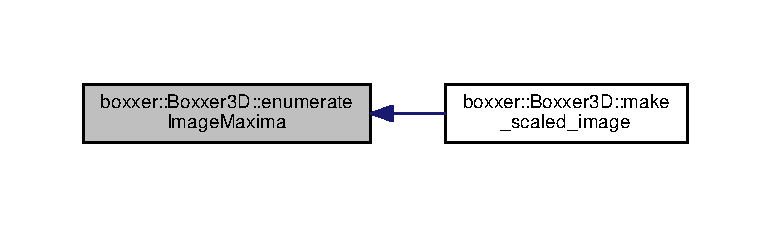
\includegraphics[width=350pt]{classboxxer_1_1Boxxer3D_a2fbe5c1f5d3b705ddcca7d13a92f9283_icgraph}
\end{center}
\end{figure}


\index{boxxer\+::\+Boxxer3D@{boxxer\+::\+Boxxer3D}!filter\+DoG@{filter\+DoG}}
\index{filter\+DoG@{filter\+DoG}!boxxer\+::\+Boxxer3D@{boxxer\+::\+Boxxer3D}}
\paragraph[{\texorpdfstring{filter\+Do\+G(const Image\+Stack\+T \&im, Image\+Stack\+T \&fim, const Vec\+T \&sigma, Float\+T sigma\+\_\+ratio)}{filterDoG(const ImageStackT &im, ImageStackT &fim, const VecT &sigma, FloatT sigma_ratio)}}]{\setlength{\rightskip}{0pt plus 5cm}template$<$class FloatT  = float, class IdxT  = uint32\+\_\+t$>$ static void {\bf boxxer\+::\+Boxxer3D}$<$ FloatT, IdxT $>$\+::filter\+DoG (
\begin{DoxyParamCaption}
\item[{const {\bf Image\+StackT} \&}]{im, }
\item[{{\bf Image\+StackT} \&}]{fim, }
\item[{const {\bf VecT} \&}]{sigma, }
\item[{FloatT}]{sigma\+\_\+ratio}
\end{DoxyParamCaption}
)\hspace{0.3cm}{\ttfamily [static]}}\hypertarget{classboxxer_1_1Boxxer3D_a523dff6ee90ba9f6e6bb0e8e4258a905}{}\label{classboxxer_1_1Boxxer3D_a523dff6ee90ba9f6e6bb0e8e4258a905}


Referenced by boxxer\+::\+Boxxer3\+D$<$ Float\+T, Idx\+T $>$\+::make\+\_\+scaled\+\_\+image().



Here is the caller graph for this function\+:\nopagebreak
\begin{figure}[H]
\begin{center}
\leavevmode
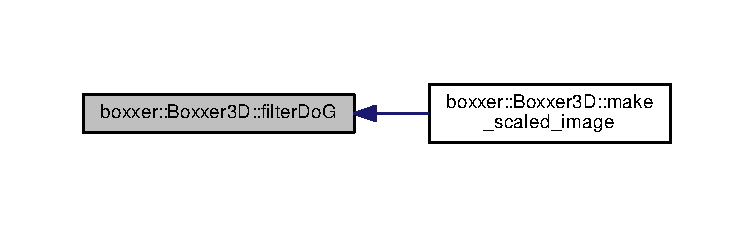
\includegraphics[width=350pt]{classboxxer_1_1Boxxer3D_a523dff6ee90ba9f6e6bb0e8e4258a905_icgraph}
\end{center}
\end{figure}


\index{boxxer\+::\+Boxxer3D@{boxxer\+::\+Boxxer3D}!filter\+Gauss@{filter\+Gauss}}
\index{filter\+Gauss@{filter\+Gauss}!boxxer\+::\+Boxxer3D@{boxxer\+::\+Boxxer3D}}
\paragraph[{\texorpdfstring{filter\+Gauss(const Image\+Stack\+T \&im, Image\+Stack\+T \&fim, const Vec\+T \&sigma)}{filterGauss(const ImageStackT &im, ImageStackT &fim, const VecT &sigma)}}]{\setlength{\rightskip}{0pt plus 5cm}template$<$class FloatT  = float, class IdxT  = uint32\+\_\+t$>$ static void {\bf boxxer\+::\+Boxxer3D}$<$ FloatT, IdxT $>$\+::filter\+Gauss (
\begin{DoxyParamCaption}
\item[{const {\bf Image\+StackT} \&}]{im, }
\item[{{\bf Image\+StackT} \&}]{fim, }
\item[{const {\bf VecT} \&}]{sigma}
\end{DoxyParamCaption}
)\hspace{0.3cm}{\ttfamily [static]}}\hypertarget{classboxxer_1_1Boxxer3D_a210c289db79c6db6596df92d77052f47}{}\label{classboxxer_1_1Boxxer3D_a210c289db79c6db6596df92d77052f47}


Referenced by boxxer\+::\+Boxxer3\+D$<$ Float\+T, Idx\+T $>$\+::make\+\_\+scaled\+\_\+image().



Here is the caller graph for this function\+:\nopagebreak
\begin{figure}[H]
\begin{center}
\leavevmode
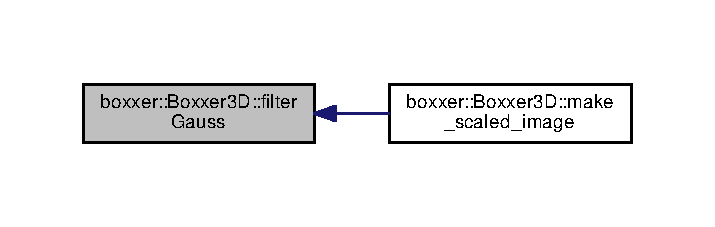
\includegraphics[width=343pt]{classboxxer_1_1Boxxer3D_a210c289db79c6db6596df92d77052f47_icgraph}
\end{center}
\end{figure}


\index{boxxer\+::\+Boxxer3D@{boxxer\+::\+Boxxer3D}!filter\+LoG@{filter\+LoG}}
\index{filter\+LoG@{filter\+LoG}!boxxer\+::\+Boxxer3D@{boxxer\+::\+Boxxer3D}}
\paragraph[{\texorpdfstring{filter\+Lo\+G(const Image\+Stack\+T \&im, Image\+Stack\+T \&fim, const Vec\+T \&sigma)}{filterLoG(const ImageStackT &im, ImageStackT &fim, const VecT &sigma)}}]{\setlength{\rightskip}{0pt plus 5cm}template$<$class FloatT  = float, class IdxT  = uint32\+\_\+t$>$ static void {\bf boxxer\+::\+Boxxer3D}$<$ FloatT, IdxT $>$\+::filter\+LoG (
\begin{DoxyParamCaption}
\item[{const {\bf Image\+StackT} \&}]{im, }
\item[{{\bf Image\+StackT} \&}]{fim, }
\item[{const {\bf VecT} \&}]{sigma}
\end{DoxyParamCaption}
)\hspace{0.3cm}{\ttfamily [static]}}\hypertarget{classboxxer_1_1Boxxer3D_ad242333de1472fea719db9958dfe6f46}{}\label{classboxxer_1_1Boxxer3D_ad242333de1472fea719db9958dfe6f46}


Referenced by boxxer\+::\+Boxxer3\+D$<$ Float\+T, Idx\+T $>$\+::make\+\_\+scaled\+\_\+image().



Here is the caller graph for this function\+:\nopagebreak
\begin{figure}[H]
\begin{center}
\leavevmode
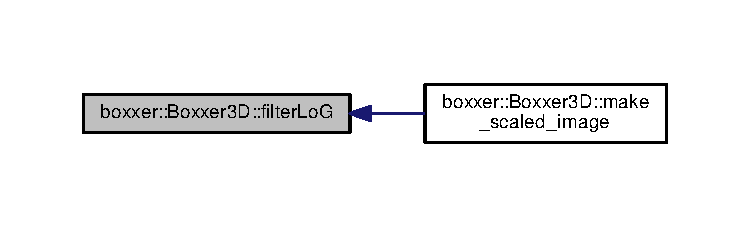
\includegraphics[width=350pt]{classboxxer_1_1Boxxer3D_ad242333de1472fea719db9958dfe6f46_icgraph}
\end{center}
\end{figure}


\index{boxxer\+::\+Boxxer3D@{boxxer\+::\+Boxxer3D}!filter\+Scaled\+DoG@{filter\+Scaled\+DoG}}
\index{filter\+Scaled\+DoG@{filter\+Scaled\+DoG}!boxxer\+::\+Boxxer3D@{boxxer\+::\+Boxxer3D}}
\paragraph[{\texorpdfstring{filter\+Scaled\+Do\+G(const Image\+T \&im, Scaled\+Image\+T \&fim)}{filterScaledDoG(const ImageT &im, ScaledImageT &fim)}}]{\setlength{\rightskip}{0pt plus 5cm}template$<$class FloatT  = float, class IdxT  = uint32\+\_\+t$>$ void {\bf boxxer\+::\+Boxxer3D}$<$ FloatT, IdxT $>$\+::filter\+Scaled\+DoG (
\begin{DoxyParamCaption}
\item[{const {\bf ImageT} \&}]{im, }
\item[{{\bf Scaled\+ImageT} \&}]{fim}
\end{DoxyParamCaption}
)}\hypertarget{classboxxer_1_1Boxxer3D_ae1e5a4f23ea5909e10e0545e56e334df}{}\label{classboxxer_1_1Boxxer3D_ae1e5a4f23ea5909e10e0545e56e334df}
\index{boxxer\+::\+Boxxer3D@{boxxer\+::\+Boxxer3D}!filter\+Scaled\+LoG@{filter\+Scaled\+LoG}}
\index{filter\+Scaled\+LoG@{filter\+Scaled\+LoG}!boxxer\+::\+Boxxer3D@{boxxer\+::\+Boxxer3D}}
\paragraph[{\texorpdfstring{filter\+Scaled\+Lo\+G(const Image\+T \&im, Scaled\+Image\+T \&fim)}{filterScaledLoG(const ImageT &im, ScaledImageT &fim)}}]{\setlength{\rightskip}{0pt plus 5cm}template$<$class FloatT  = float, class IdxT  = uint32\+\_\+t$>$ void {\bf boxxer\+::\+Boxxer3D}$<$ FloatT, IdxT $>$\+::filter\+Scaled\+LoG (
\begin{DoxyParamCaption}
\item[{const {\bf ImageT} \&}]{im, }
\item[{{\bf Scaled\+ImageT} \&}]{fim}
\end{DoxyParamCaption}
)}\hypertarget{classboxxer_1_1Boxxer3D_a54ce058d4f00b44b40808cdc964ea7f5}{}\label{classboxxer_1_1Boxxer3D_a54ce058d4f00b44b40808cdc964ea7f5}
\index{boxxer\+::\+Boxxer3D@{boxxer\+::\+Boxxer3D}!make\+\_\+image@{make\+\_\+image}}
\index{make\+\_\+image@{make\+\_\+image}!boxxer\+::\+Boxxer3D@{boxxer\+::\+Boxxer3D}}
\paragraph[{\texorpdfstring{make\+\_\+image() const }{make_image() const }}]{\setlength{\rightskip}{0pt plus 5cm}template$<$class FloatT  = float, class IdxT  = uint32\+\_\+t$>$ {\bf ImageT} {\bf boxxer\+::\+Boxxer3D}$<$ FloatT, IdxT $>$\+::make\+\_\+image (
\begin{DoxyParamCaption}
{}
\end{DoxyParamCaption}
) const\hspace{0.3cm}{\ttfamily [inline]}}\hypertarget{classboxxer_1_1Boxxer3D_a8e86e20a67d0275319436b6d76f8c765}{}\label{classboxxer_1_1Boxxer3D_a8e86e20a67d0275319436b6d76f8c765}


Definition at line 55 of file Boxxer3\+D.\+h.



References boxxer\+::\+Boxxer3\+D$<$ Float\+T, Idx\+T $>$\+::imsize.

\index{boxxer\+::\+Boxxer3D@{boxxer\+::\+Boxxer3D}!make\+\_\+image\+\_\+stack@{make\+\_\+image\+\_\+stack}}
\index{make\+\_\+image\+\_\+stack@{make\+\_\+image\+\_\+stack}!boxxer\+::\+Boxxer3D@{boxxer\+::\+Boxxer3D}}
\paragraph[{\texorpdfstring{make\+\_\+image\+\_\+stack(\+Idx\+T n\+T) const }{make_image_stack(IdxT nT) const }}]{\setlength{\rightskip}{0pt plus 5cm}template$<$class FloatT  = float, class IdxT  = uint32\+\_\+t$>$ {\bf Image\+StackT} {\bf boxxer\+::\+Boxxer3D}$<$ FloatT, IdxT $>$\+::make\+\_\+image\+\_\+stack (
\begin{DoxyParamCaption}
\item[{IdxT}]{nT}
\end{DoxyParamCaption}
) const\hspace{0.3cm}{\ttfamily [inline]}}\hypertarget{classboxxer_1_1Boxxer3D_a25c358eb9570f8a32d892e89b4b02e90}{}\label{classboxxer_1_1Boxxer3D_a25c358eb9570f8a32d892e89b4b02e90}


Definition at line 56 of file Boxxer3\+D.\+h.



References boxxer\+::\+Boxxer3\+D$<$ Float\+T, Idx\+T $>$\+::imsize.

\index{boxxer\+::\+Boxxer3D@{boxxer\+::\+Boxxer3D}!make\+\_\+scaled\+\_\+image@{make\+\_\+scaled\+\_\+image}}
\index{make\+\_\+scaled\+\_\+image@{make\+\_\+scaled\+\_\+image}!boxxer\+::\+Boxxer3D@{boxxer\+::\+Boxxer3D}}
\paragraph[{\texorpdfstring{make\+\_\+scaled\+\_\+image() const }{make_scaled_image() const }}]{\setlength{\rightskip}{0pt plus 5cm}template$<$class FloatT  = float, class IdxT  = uint32\+\_\+t$>$ {\bf Scaled\+ImageT} {\bf boxxer\+::\+Boxxer3D}$<$ FloatT, IdxT $>$\+::make\+\_\+scaled\+\_\+image (
\begin{DoxyParamCaption}
{}
\end{DoxyParamCaption}
) const\hspace{0.3cm}{\ttfamily [inline]}}\hypertarget{classboxxer_1_1Boxxer3D_a3bc9609e6bdb4a6aac10aea313b70b12}{}\label{classboxxer_1_1Boxxer3D_a3bc9609e6bdb4a6aac10aea313b70b12}


Definition at line 57 of file Boxxer3\+D.\+h.



References boxxer\+::\+Boxxer3\+D$<$ Float\+T, Idx\+T $>$\+::check\+Maxima(), boxxer\+::\+Boxxer3\+D$<$ Float\+T, Idx\+T $>$\+::enumerate\+Image\+Maxima(), boxxer\+::\+Boxxer3\+D$<$ Float\+T, Idx\+T $>$\+::filter\+Do\+G(), boxxer\+::\+Boxxer3\+D$<$ Float\+T, Idx\+T $>$\+::filter\+Gauss(), boxxer\+::\+Boxxer3\+D$<$ Float\+T, Idx\+T $>$\+::filter\+Lo\+G(), and boxxer\+::\+Boxxer3\+D$<$ Float\+T, Idx\+T $>$\+::imsize.



Here is the call graph for this function\+:\nopagebreak
\begin{figure}[H]
\begin{center}
\leavevmode
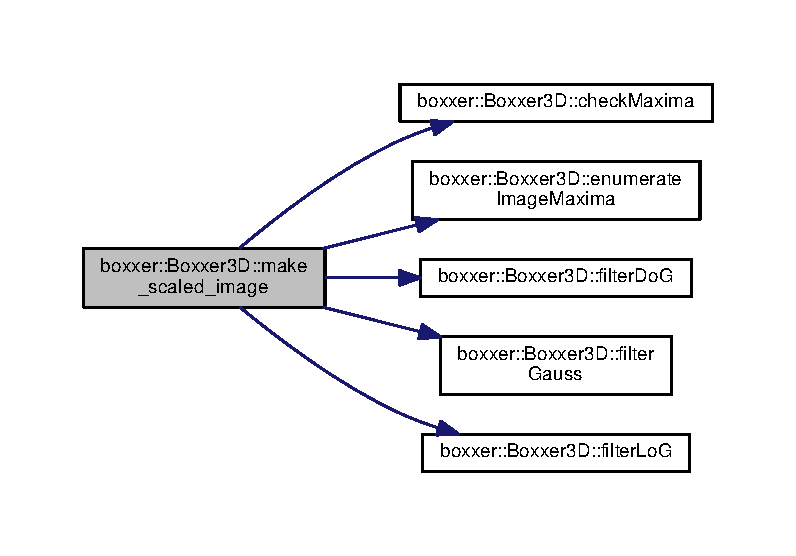
\includegraphics[width=350pt]{classboxxer_1_1Boxxer3D_a3bc9609e6bdb4a6aac10aea313b70b12_cgraph}
\end{center}
\end{figure}


\index{boxxer\+::\+Boxxer3D@{boxxer\+::\+Boxxer3D}!scale\+Space\+Do\+G\+Maxima@{scale\+Space\+Do\+G\+Maxima}}
\index{scale\+Space\+Do\+G\+Maxima@{scale\+Space\+Do\+G\+Maxima}!boxxer\+::\+Boxxer3D@{boxxer\+::\+Boxxer3D}}
\paragraph[{\texorpdfstring{scale\+Space\+Do\+G\+Maxima(const Image\+Stack\+T \&im, I\+Mat\+T \&maxima, Vec\+T \&max\+\_\+vals, Idx\+T neighborhood\+\_\+size, Idx\+T scale\+\_\+neighborhood\+\_\+size)}{scaleSpaceDoGMaxima(const ImageStackT &im, IMatT &maxima, VecT &max_vals, IdxT neighborhood_size, IdxT scale_neighborhood_size)}}]{\setlength{\rightskip}{0pt plus 5cm}template$<$class FloatT  = float, class IdxT  = uint32\+\_\+t$>$ IdxT {\bf boxxer\+::\+Boxxer3D}$<$ FloatT, IdxT $>$\+::scale\+Space\+Do\+G\+Maxima (
\begin{DoxyParamCaption}
\item[{const {\bf Image\+StackT} \&}]{im, }
\item[{{\bf I\+MatT} \&}]{maxima, }
\item[{{\bf VecT} \&}]{max\+\_\+vals, }
\item[{IdxT}]{neighborhood\+\_\+size, }
\item[{IdxT}]{scale\+\_\+neighborhood\+\_\+size}
\end{DoxyParamCaption}
)}\hypertarget{classboxxer_1_1Boxxer3D_a66040edbfb27cdc2d73be9789b7ca676}{}\label{classboxxer_1_1Boxxer3D_a66040edbfb27cdc2d73be9789b7ca676}
\index{boxxer\+::\+Boxxer3D@{boxxer\+::\+Boxxer3D}!scale\+Space\+Lo\+G\+Maxima@{scale\+Space\+Lo\+G\+Maxima}}
\index{scale\+Space\+Lo\+G\+Maxima@{scale\+Space\+Lo\+G\+Maxima}!boxxer\+::\+Boxxer3D@{boxxer\+::\+Boxxer3D}}
\paragraph[{\texorpdfstring{scale\+Space\+Lo\+G\+Maxima(const Image\+Stack\+T \&im, I\+Mat\+T \&maxima, Vec\+T \&max\+\_\+vals, Idx\+T neighborhood\+\_\+size, Idx\+T scale\+\_\+neighborhood\+\_\+size)}{scaleSpaceLoGMaxima(const ImageStackT &im, IMatT &maxima, VecT &max_vals, IdxT neighborhood_size, IdxT scale_neighborhood_size)}}]{\setlength{\rightskip}{0pt plus 5cm}template$<$class FloatT  = float, class IdxT  = uint32\+\_\+t$>$ IdxT {\bf boxxer\+::\+Boxxer3D}$<$ FloatT, IdxT $>$\+::scale\+Space\+Lo\+G\+Maxima (
\begin{DoxyParamCaption}
\item[{const {\bf Image\+StackT} \&}]{im, }
\item[{{\bf I\+MatT} \&}]{maxima, }
\item[{{\bf VecT} \&}]{max\+\_\+vals, }
\item[{IdxT}]{neighborhood\+\_\+size, }
\item[{IdxT}]{scale\+\_\+neighborhood\+\_\+size}
\end{DoxyParamCaption}
)}\hypertarget{classboxxer_1_1Boxxer3D_aa3a28765766e21dc7b994da8c056fe47}{}\label{classboxxer_1_1Boxxer3D_aa3a28765766e21dc7b994da8c056fe47}
\index{boxxer\+::\+Boxxer3D@{boxxer\+::\+Boxxer3D}!set\+Do\+G\+Sigma\+Ratio@{set\+Do\+G\+Sigma\+Ratio}}
\index{set\+Do\+G\+Sigma\+Ratio@{set\+Do\+G\+Sigma\+Ratio}!boxxer\+::\+Boxxer3D@{boxxer\+::\+Boxxer3D}}
\paragraph[{\texorpdfstring{set\+Do\+G\+Sigma\+Ratio(\+Float\+T sigma\+\_\+ratio)}{setDoGSigmaRatio(FloatT sigma_ratio)}}]{\setlength{\rightskip}{0pt plus 5cm}template$<$class FloatT  = float, class IdxT  = uint32\+\_\+t$>$ void {\bf boxxer\+::\+Boxxer3D}$<$ FloatT, IdxT $>$\+::set\+Do\+G\+Sigma\+Ratio (
\begin{DoxyParamCaption}
\item[{FloatT}]{sigma\+\_\+ratio}
\end{DoxyParamCaption}
)}\hypertarget{classboxxer_1_1Boxxer3D_a22933f928d48cfa58dbada555d8a1d1e}{}\label{classboxxer_1_1Boxxer3D_a22933f928d48cfa58dbada555d8a1d1e}


\subsubsection{Member Data Documentation}
\index{boxxer\+::\+Boxxer3D@{boxxer\+::\+Boxxer3D}!Default\+Sigma\+Ratio@{Default\+Sigma\+Ratio}}
\index{Default\+Sigma\+Ratio@{Default\+Sigma\+Ratio}!boxxer\+::\+Boxxer3D@{boxxer\+::\+Boxxer3D}}
\paragraph[{\texorpdfstring{Default\+Sigma\+Ratio}{DefaultSigmaRatio}}]{\setlength{\rightskip}{0pt plus 5cm}template$<$class FloatT  = float, class IdxT  = uint32\+\_\+t$>$ const FloatT {\bf boxxer\+::\+Boxxer3D}$<$ FloatT, IdxT $>$\+::Default\+Sigma\+Ratio\hspace{0.3cm}{\ttfamily [static]}}\hypertarget{classboxxer_1_1Boxxer3D_a8a489401adebfc449a1e9390dcdfbbf4}{}\label{classboxxer_1_1Boxxer3D_a8a489401adebfc449a1e9390dcdfbbf4}


Definition at line 38 of file Boxxer3\+D.\+h.

\index{boxxer\+::\+Boxxer3D@{boxxer\+::\+Boxxer3D}!dim@{dim}}
\index{dim@{dim}!boxxer\+::\+Boxxer3D@{boxxer\+::\+Boxxer3D}}
\paragraph[{\texorpdfstring{dim}{dim}}]{\setlength{\rightskip}{0pt plus 5cm}template$<$class FloatT  = float, class IdxT  = uint32\+\_\+t$>$ const IdxT {\bf boxxer\+::\+Boxxer3D}$<$ FloatT, IdxT $>$\+::dim\hspace{0.3cm}{\ttfamily [static]}}\hypertarget{classboxxer_1_1Boxxer3D_a8ae92f1badc81d59b178c12fb339e251}{}\label{classboxxer_1_1Boxxer3D_a8ae92f1badc81d59b178c12fb339e251}


Definition at line 39 of file Boxxer3\+D.\+h.

\index{boxxer\+::\+Boxxer3D@{boxxer\+::\+Boxxer3D}!imsize@{imsize}}
\index{imsize@{imsize}!boxxer\+::\+Boxxer3D@{boxxer\+::\+Boxxer3D}}
\paragraph[{\texorpdfstring{imsize}{imsize}}]{\setlength{\rightskip}{0pt plus 5cm}template$<$class FloatT  = float, class IdxT  = uint32\+\_\+t$>$ {\bf I\+VecT} {\bf boxxer\+::\+Boxxer3D}$<$ FloatT, IdxT $>$\+::imsize}\hypertarget{classboxxer_1_1Boxxer3D_a236f3f4ada01376204e59f9f68d5fde6}{}\label{classboxxer_1_1Boxxer3D_a236f3f4ada01376204e59f9f68d5fde6}


Definition at line 42 of file Boxxer3\+D.\+h.



Referenced by boxxer\+::\+Boxxer3\+D$<$ Float\+T, Idx\+T $>$\+::make\+\_\+image(), boxxer\+::\+Boxxer3\+D$<$ Float\+T, Idx\+T $>$\+::make\+\_\+image\+\_\+stack(), and boxxer\+::\+Boxxer3\+D$<$ Float\+T, Idx\+T $>$\+::make\+\_\+scaled\+\_\+image().

\index{boxxer\+::\+Boxxer3D@{boxxer\+::\+Boxxer3D}!n\+Scales@{n\+Scales}}
\index{n\+Scales@{n\+Scales}!boxxer\+::\+Boxxer3D@{boxxer\+::\+Boxxer3D}}
\paragraph[{\texorpdfstring{n\+Scales}{nScales}}]{\setlength{\rightskip}{0pt plus 5cm}template$<$class FloatT  = float, class IdxT  = uint32\+\_\+t$>$ IdxT {\bf boxxer\+::\+Boxxer3D}$<$ FloatT, IdxT $>$\+::n\+Scales}\hypertarget{classboxxer_1_1Boxxer3D_a344ef289cd330d4353c4605f2c2e2bbc}{}\label{classboxxer_1_1Boxxer3D_a344ef289cd330d4353c4605f2c2e2bbc}


Definition at line 41 of file Boxxer3\+D.\+h.

\index{boxxer\+::\+Boxxer3D@{boxxer\+::\+Boxxer3D}!sigma@{sigma}}
\index{sigma@{sigma}!boxxer\+::\+Boxxer3D@{boxxer\+::\+Boxxer3D}}
\paragraph[{\texorpdfstring{sigma}{sigma}}]{\setlength{\rightskip}{0pt plus 5cm}template$<$class FloatT  = float, class IdxT  = uint32\+\_\+t$>$ {\bf MatT} {\bf boxxer\+::\+Boxxer3D}$<$ FloatT, IdxT $>$\+::sigma}\hypertarget{classboxxer_1_1Boxxer3D_a5df6b670e57ee7b6c2396650f6caba86}{}\label{classboxxer_1_1Boxxer3D_a5df6b670e57ee7b6c2396650f6caba86}


Definition at line 43 of file Boxxer3\+D.\+h.

\index{boxxer\+::\+Boxxer3D@{boxxer\+::\+Boxxer3D}!sigma\+\_\+ratio@{sigma\+\_\+ratio}}
\index{sigma\+\_\+ratio@{sigma\+\_\+ratio}!boxxer\+::\+Boxxer3D@{boxxer\+::\+Boxxer3D}}
\paragraph[{\texorpdfstring{sigma\+\_\+ratio}{sigma_ratio}}]{\setlength{\rightskip}{0pt plus 5cm}template$<$class FloatT  = float, class IdxT  = uint32\+\_\+t$>$ FloatT {\bf boxxer\+::\+Boxxer3D}$<$ FloatT, IdxT $>$\+::sigma\+\_\+ratio}\hypertarget{classboxxer_1_1Boxxer3D_a63a9a0d9c56c11f34c7f2c80e0556335}{}\label{classboxxer_1_1Boxxer3D_a63a9a0d9c56c11f34c7f2c80e0556335}


Definition at line 45 of file Boxxer3\+D.\+h.



The documentation for this class was generated from the following file\+:\begin{DoxyCompactItemize}
\item 
\hyperlink{Boxxer3D_8h}{Boxxer3\+D.\+h}\end{DoxyCompactItemize}

\hypertarget{classboxxer_1_1DoGFilter2D}{}\subsection{boxxer\+:\+:Do\+G\+Filter2D$<$ FloatT, IdxT $>$ Class Template Reference}
\label{classboxxer_1_1DoGFilter2D}\index{boxxer\+::\+Do\+G\+Filter2\+D$<$ Float\+T, Idx\+T $>$@{boxxer\+::\+Do\+G\+Filter2\+D$<$ Float\+T, Idx\+T $>$}}


{\ttfamily \#include $<$/home/travis/build/markjolah/\+Boxxer/include/\+Boxxer/\+Gauss\+Filter.\+h$>$}



Inheritance diagram for boxxer\+:\+:Do\+G\+Filter2D$<$ FloatT, IdxT $>$\+:\nopagebreak
\begin{figure}[H]
\begin{center}
\leavevmode
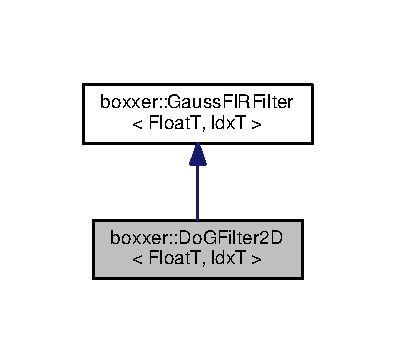
\includegraphics[width=190pt]{classboxxer_1_1DoGFilter2D__inherit__graph}
\end{center}
\end{figure}


Collaboration diagram for boxxer\+:\+:Do\+G\+Filter2D$<$ FloatT, IdxT $>$\+:\nopagebreak
\begin{figure}[H]
\begin{center}
\leavevmode
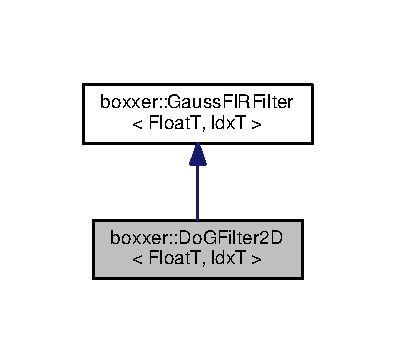
\includegraphics[width=190pt]{classboxxer_1_1DoGFilter2D__coll__graph}
\end{center}
\end{figure}
\subsubsection*{Public Types}
\begin{DoxyCompactItemize}
\item 
using \hyperlink{classboxxer_1_1DoGFilter2D_a3cf901b2a5f6254149ca635244176c7f}{I\+VecT} = typename \hyperlink{classboxxer_1_1GaussFIRFilter}{Gauss\+F\+I\+R\+Filter}$<$ FloatT, IdxT $>$\+::\hyperlink{classboxxer_1_1GaussFIRFilter_a0083c8c9ab6032dd458b4dc93852c2b8}{I\+VecT}
\item 
using \hyperlink{classboxxer_1_1DoGFilter2D_a77bd6efdb8dc5643aa30c2575c9da261}{VecT} = typename \hyperlink{classboxxer_1_1GaussFIRFilter}{Gauss\+F\+I\+R\+Filter}$<$ FloatT, IdxT $>$\+::\hyperlink{classboxxer_1_1DoGFilter2D_a77bd6efdb8dc5643aa30c2575c9da261}{VecT}
\item 
using \hyperlink{classboxxer_1_1DoGFilter2D_aef097cf982b1705c47b2e2b34baf1bb1}{ImageT} = arma\+::\+Mat$<$ FloatT $>$
\item 
using \hyperlink{classboxxer_1_1GaussFIRFilter_a83cf4c7f4782f69918c0e0883fff5412}{MatT} = arma\+::\+Mat$<$ FloatT $>$
\end{DoxyCompactItemize}
\subsubsection*{Public Member Functions}
\begin{DoxyCompactItemize}
\item 
\hyperlink{classboxxer_1_1DoGFilter2D_ab423fa2c4bb16faea4c33a92ab08411c}{Do\+G\+Filter2D} (const \hyperlink{classboxxer_1_1GaussFIRFilter_a0083c8c9ab6032dd458b4dc93852c2b8}{I\+VecT} \&\hyperlink{classboxxer_1_1GaussFIRFilter_ac0d4e19bb2be3e8913e77283e7e4317e}{size}, const \hyperlink{classboxxer_1_1DoGFilter2D_a77bd6efdb8dc5643aa30c2575c9da261}{VecT} \&\hyperlink{classboxxer_1_1GaussFIRFilter_a66ced06c688fd544d5f1f8be39aa2125}{sigma}, FloatT \hyperlink{classboxxer_1_1DoGFilter2D_a68e3d95c06f7d41782be2d1a1db96ace}{sigma\+\_\+ratio})
\item 
\hyperlink{classboxxer_1_1DoGFilter2D_aa8b99c2a75dfa10fd171bf2661f05c6a}{Do\+G\+Filter2D} (const \hyperlink{classboxxer_1_1GaussFIRFilter_a0083c8c9ab6032dd458b4dc93852c2b8}{I\+VecT} \&\hyperlink{classboxxer_1_1GaussFIRFilter_ac0d4e19bb2be3e8913e77283e7e4317e}{size}, const \hyperlink{classboxxer_1_1DoGFilter2D_a77bd6efdb8dc5643aa30c2575c9da261}{VecT} \&\hyperlink{classboxxer_1_1GaussFIRFilter_a66ced06c688fd544d5f1f8be39aa2125}{sigma}, FloatT \hyperlink{classboxxer_1_1DoGFilter2D_a68e3d95c06f7d41782be2d1a1db96ace}{sigma\+\_\+ratio}, const \hyperlink{classboxxer_1_1GaussFIRFilter_a0083c8c9ab6032dd458b4dc93852c2b8}{I\+VecT} \&kernel\+\_\+hw)
\item 
void \hyperlink{classboxxer_1_1DoGFilter2D_a3fcf9339a299ad57e3427fce9d59661a}{set\+\_\+kernel\+\_\+hw} (const \hyperlink{classboxxer_1_1GaussFIRFilter_a0083c8c9ab6032dd458b4dc93852c2b8}{I\+VecT} \&kernel\+\_\+half\+\_\+width)
\item 
void \hyperlink{classboxxer_1_1DoGFilter2D_af6c4276ff6195d6052d834d9c7fbb04c}{set\+\_\+sigma\+\_\+ratio} (FloatT \hyperlink{classboxxer_1_1DoGFilter2D_a68e3d95c06f7d41782be2d1a1db96ace}{sigma\+\_\+ratio})
\item 
\hyperlink{classboxxer_1_1DoGFilter2D_aef097cf982b1705c47b2e2b34baf1bb1}{ImageT} \hyperlink{classboxxer_1_1DoGFilter2D_a78c7c1791abff3bc665bac7becc0dec1}{make\+\_\+image} () const 
\item 
void \hyperlink{classboxxer_1_1DoGFilter2D_a2d5cf92732000f8c444b32041b89fe00}{filter} (const \hyperlink{classboxxer_1_1DoGFilter2D_aef097cf982b1705c47b2e2b34baf1bb1}{ImageT} \&im, \hyperlink{classboxxer_1_1DoGFilter2D_aef097cf982b1705c47b2e2b34baf1bb1}{ImageT} \&out)
\item 
void \hyperlink{classboxxer_1_1DoGFilter2D_a560b334f15bc28f411b065b22ffd4bb7}{test\+\_\+filter} (const \hyperlink{classboxxer_1_1DoGFilter2D_aef097cf982b1705c47b2e2b34baf1bb1}{ImageT} \&im)
\end{DoxyCompactItemize}
\subsubsection*{Static Public Member Functions}
\begin{DoxyCompactItemize}
\item 
static \hyperlink{classboxxer_1_1DoGFilter2D_a77bd6efdb8dc5643aa30c2575c9da261}{VecT} \hyperlink{classboxxer_1_1GaussFIRFilter_a5dd6de5fe82092ec30141ab920d75dfd}{compute\+\_\+\+Gauss\+\_\+\+F\+I\+R\+\_\+kernel} (FloatT \hyperlink{classboxxer_1_1GaussFIRFilter_a66ced06c688fd544d5f1f8be39aa2125}{sigma}, IdxT \hyperlink{classboxxer_1_1GaussFIRFilter_ae17a4e137303e452a9223ba34825e0da}{hw})
\item 
static \hyperlink{classboxxer_1_1DoGFilter2D_a77bd6efdb8dc5643aa30c2575c9da261}{VecT} \hyperlink{classboxxer_1_1GaussFIRFilter_ad6a618b47db57b570278cc57b05d8c03}{compute\+\_\+\+Lo\+G\+\_\+\+F\+I\+R\+\_\+kernel} (FloatT \hyperlink{classboxxer_1_1GaussFIRFilter_a66ced06c688fd544d5f1f8be39aa2125}{sigma}, IdxT \hyperlink{classboxxer_1_1GaussFIRFilter_ae17a4e137303e452a9223ba34825e0da}{hw})
\end{DoxyCompactItemize}
\subsubsection*{Public Attributes}
\begin{DoxyCompactItemize}
\item 
FloatT \hyperlink{classboxxer_1_1DoGFilter2D_a68e3d95c06f7d41782be2d1a1db96ace}{sigma\+\_\+ratio}
\item 
IdxT \hyperlink{classboxxer_1_1GaussFIRFilter_ac7adcd4d8f8efee00a65262f596c8eda}{dim}
\item 
\hyperlink{classboxxer_1_1GaussFIRFilter_a0083c8c9ab6032dd458b4dc93852c2b8}{I\+VecT} \hyperlink{classboxxer_1_1GaussFIRFilter_ac0d4e19bb2be3e8913e77283e7e4317e}{size}
\item 
\hyperlink{classboxxer_1_1DoGFilter2D_a77bd6efdb8dc5643aa30c2575c9da261}{VecT} \hyperlink{classboxxer_1_1GaussFIRFilter_a66ced06c688fd544d5f1f8be39aa2125}{sigma}
\item 
\hyperlink{classboxxer_1_1GaussFIRFilter_a0083c8c9ab6032dd458b4dc93852c2b8}{I\+VecT} \hyperlink{classboxxer_1_1GaussFIRFilter_ae17a4e137303e452a9223ba34825e0da}{hw}
\end{DoxyCompactItemize}
\subsubsection*{Static Protected Attributes}
\begin{DoxyCompactItemize}
\item 
static const IdxT \hyperlink{classboxxer_1_1GaussFIRFilter_a7f85e018f78753ee4fedf65c04b0c65a}{max\+\_\+kernel\+\_\+hw}
\item 
static const FloatT \hyperlink{classboxxer_1_1GaussFIRFilter_a72b51cd7549510735179cb9c94f5f43f}{default\+\_\+sigma\+\_\+hw\+\_\+ratio}
\end{DoxyCompactItemize}
\subsubsection*{Friends}
\begin{DoxyCompactItemize}
\item 
{\footnotesize template$<$class Float\+T\+\_\+ , class Idx\+T\+\_\+ $>$ }\\std\+::ostream \& \hyperlink{classboxxer_1_1DoGFilter2D_a5226e7e31cc72aeef946cd5d60bc3f49}{operator$<$$<$} (std\+::ostream \&out, const \hyperlink{classboxxer_1_1DoGFilter2D}{Do\+G\+Filter2D}$<$ Float\+T\+\_\+, Idx\+T\+\_\+ $>$ \&filt)
\end{DoxyCompactItemize}


\subsubsection{Detailed Description}
\subsubsection*{template$<$class FloatT = float, class IdxT = uint32\+\_\+t$>$\\*
class boxxer\+::\+Do\+G\+Filter2\+D$<$ Float\+T, Idx\+T $>$}



Definition at line 70 of file Gauss\+Filter.\+h.



\subsubsection{Member Typedef Documentation}
\index{boxxer\+::\+Do\+G\+Filter2D@{boxxer\+::\+Do\+G\+Filter2D}!ImageT@{ImageT}}
\index{ImageT@{ImageT}!boxxer\+::\+Do\+G\+Filter2D@{boxxer\+::\+Do\+G\+Filter2D}}
\paragraph[{\texorpdfstring{ImageT}{ImageT}}]{\setlength{\rightskip}{0pt plus 5cm}template$<$class FloatT  = float, class IdxT  = uint32\+\_\+t$>$ using {\bf boxxer\+::\+Do\+G\+Filter2D}$<$ FloatT, IdxT $>$\+::{\bf ImageT} =  arma\+::\+Mat$<$FloatT$>$}\hypertarget{classboxxer_1_1DoGFilter2D_aef097cf982b1705c47b2e2b34baf1bb1}{}\label{classboxxer_1_1DoGFilter2D_aef097cf982b1705c47b2e2b34baf1bb1}


Definition at line 75 of file Gauss\+Filter.\+h.

\index{boxxer\+::\+Do\+G\+Filter2D@{boxxer\+::\+Do\+G\+Filter2D}!I\+VecT@{I\+VecT}}
\index{I\+VecT@{I\+VecT}!boxxer\+::\+Do\+G\+Filter2D@{boxxer\+::\+Do\+G\+Filter2D}}
\paragraph[{\texorpdfstring{I\+VecT}{IVecT}}]{\setlength{\rightskip}{0pt plus 5cm}template$<$class FloatT  = float, class IdxT  = uint32\+\_\+t$>$ using {\bf boxxer\+::\+Do\+G\+Filter2D}$<$ FloatT, IdxT $>$\+::{\bf I\+VecT} =  typename {\bf Gauss\+F\+I\+R\+Filter}$<$FloatT,IdxT$>$\+::{\bf I\+VecT}}\hypertarget{classboxxer_1_1DoGFilter2D_a3cf901b2a5f6254149ca635244176c7f}{}\label{classboxxer_1_1DoGFilter2D_a3cf901b2a5f6254149ca635244176c7f}


Definition at line 73 of file Gauss\+Filter.\+h.

\index{boxxer\+::\+Do\+G\+Filter2D@{boxxer\+::\+Do\+G\+Filter2D}!MatT@{MatT}}
\index{MatT@{MatT}!boxxer\+::\+Do\+G\+Filter2D@{boxxer\+::\+Do\+G\+Filter2D}}
\paragraph[{\texorpdfstring{MatT}{MatT}}]{\setlength{\rightskip}{0pt plus 5cm}template$<$class FloatT = float, class IdxT = uint32\+\_\+t$>$ using {\bf boxxer\+::\+Gauss\+F\+I\+R\+Filter}$<$ FloatT, IdxT $>$\+::{\bf MatT} =  arma\+::\+Mat$<$FloatT$>$\hspace{0.3cm}{\ttfamily [inherited]}}\hypertarget{classboxxer_1_1GaussFIRFilter_a83cf4c7f4782f69918c0e0883fff5412}{}\label{classboxxer_1_1GaussFIRFilter_a83cf4c7f4782f69918c0e0883fff5412}


Definition at line 26 of file Gauss\+Filter.\+h.

\index{boxxer\+::\+Do\+G\+Filter2D@{boxxer\+::\+Do\+G\+Filter2D}!VecT@{VecT}}
\index{VecT@{VecT}!boxxer\+::\+Do\+G\+Filter2D@{boxxer\+::\+Do\+G\+Filter2D}}
\paragraph[{\texorpdfstring{VecT}{VecT}}]{\setlength{\rightskip}{0pt plus 5cm}template$<$class FloatT  = float, class IdxT  = uint32\+\_\+t$>$ using {\bf boxxer\+::\+Do\+G\+Filter2D}$<$ FloatT, IdxT $>$\+::{\bf VecT} =  typename {\bf Gauss\+F\+I\+R\+Filter}$<$FloatT,IdxT$>$\+::{\bf VecT}}\hypertarget{classboxxer_1_1DoGFilter2D_a77bd6efdb8dc5643aa30c2575c9da261}{}\label{classboxxer_1_1DoGFilter2D_a77bd6efdb8dc5643aa30c2575c9da261}


Definition at line 74 of file Gauss\+Filter.\+h.



\subsubsection{Constructor \& Destructor Documentation}
\index{boxxer\+::\+Do\+G\+Filter2D@{boxxer\+::\+Do\+G\+Filter2D}!Do\+G\+Filter2D@{Do\+G\+Filter2D}}
\index{Do\+G\+Filter2D@{Do\+G\+Filter2D}!boxxer\+::\+Do\+G\+Filter2D@{boxxer\+::\+Do\+G\+Filter2D}}
\paragraph[{\texorpdfstring{Do\+G\+Filter2\+D(const I\+Vec\+T \&size, const Vec\+T \&sigma, Float\+T sigma\+\_\+ratio)}{DoGFilter2D(const IVecT &size, const VecT &sigma, FloatT sigma_ratio)}}]{\setlength{\rightskip}{0pt plus 5cm}template$<$class FloatT  = float, class IdxT  = uint32\+\_\+t$>$ {\bf boxxer\+::\+Do\+G\+Filter2D}$<$ FloatT, IdxT $>$\+::{\bf Do\+G\+Filter2D} (
\begin{DoxyParamCaption}
\item[{const {\bf I\+VecT} \&}]{size, }
\item[{const {\bf VecT} \&}]{sigma, }
\item[{FloatT}]{sigma\+\_\+ratio}
\end{DoxyParamCaption}
)}\hypertarget{classboxxer_1_1DoGFilter2D_ab423fa2c4bb16faea4c33a92ab08411c}{}\label{classboxxer_1_1DoGFilter2D_ab423fa2c4bb16faea4c33a92ab08411c}
\index{boxxer\+::\+Do\+G\+Filter2D@{boxxer\+::\+Do\+G\+Filter2D}!Do\+G\+Filter2D@{Do\+G\+Filter2D}}
\index{Do\+G\+Filter2D@{Do\+G\+Filter2D}!boxxer\+::\+Do\+G\+Filter2D@{boxxer\+::\+Do\+G\+Filter2D}}
\paragraph[{\texorpdfstring{Do\+G\+Filter2\+D(const I\+Vec\+T \&size, const Vec\+T \&sigma, Float\+T sigma\+\_\+ratio, const I\+Vec\+T \&kernel\+\_\+hw)}{DoGFilter2D(const IVecT &size, const VecT &sigma, FloatT sigma_ratio, const IVecT &kernel_hw)}}]{\setlength{\rightskip}{0pt plus 5cm}template$<$class FloatT  = float, class IdxT  = uint32\+\_\+t$>$ {\bf boxxer\+::\+Do\+G\+Filter2D}$<$ FloatT, IdxT $>$\+::{\bf Do\+G\+Filter2D} (
\begin{DoxyParamCaption}
\item[{const {\bf I\+VecT} \&}]{size, }
\item[{const {\bf VecT} \&}]{sigma, }
\item[{FloatT}]{sigma\+\_\+ratio, }
\item[{const {\bf I\+VecT} \&}]{kernel\+\_\+hw}
\end{DoxyParamCaption}
)}\hypertarget{classboxxer_1_1DoGFilter2D_aa8b99c2a75dfa10fd171bf2661f05c6a}{}\label{classboxxer_1_1DoGFilter2D_aa8b99c2a75dfa10fd171bf2661f05c6a}


\subsubsection{Member Function Documentation}
\index{boxxer\+::\+Do\+G\+Filter2D@{boxxer\+::\+Do\+G\+Filter2D}!compute\+\_\+\+Gauss\+\_\+\+F\+I\+R\+\_\+kernel@{compute\+\_\+\+Gauss\+\_\+\+F\+I\+R\+\_\+kernel}}
\index{compute\+\_\+\+Gauss\+\_\+\+F\+I\+R\+\_\+kernel@{compute\+\_\+\+Gauss\+\_\+\+F\+I\+R\+\_\+kernel}!boxxer\+::\+Do\+G\+Filter2D@{boxxer\+::\+Do\+G\+Filter2D}}
\paragraph[{\texorpdfstring{compute\+\_\+\+Gauss\+\_\+\+F\+I\+R\+\_\+kernel(\+Float\+T sigma, Idx\+T hw)}{compute_Gauss_FIR_kernel(FloatT sigma, IdxT hw)}}]{\setlength{\rightskip}{0pt plus 5cm}template$<$class FloatT = float, class IdxT = uint32\+\_\+t$>$ static {\bf VecT} {\bf boxxer\+::\+Gauss\+F\+I\+R\+Filter}$<$ FloatT, IdxT $>$\+::compute\+\_\+\+Gauss\+\_\+\+F\+I\+R\+\_\+kernel (
\begin{DoxyParamCaption}
\item[{FloatT}]{sigma, }
\item[{IdxT}]{hw}
\end{DoxyParamCaption}
)\hspace{0.3cm}{\ttfamily [static]}, {\ttfamily [inherited]}}\hypertarget{classboxxer_1_1GaussFIRFilter_a5dd6de5fe82092ec30141ab920d75dfd}{}\label{classboxxer_1_1GaussFIRFilter_a5dd6de5fe82092ec30141ab920d75dfd}
\index{boxxer\+::\+Do\+G\+Filter2D@{boxxer\+::\+Do\+G\+Filter2D}!compute\+\_\+\+Lo\+G\+\_\+\+F\+I\+R\+\_\+kernel@{compute\+\_\+\+Lo\+G\+\_\+\+F\+I\+R\+\_\+kernel}}
\index{compute\+\_\+\+Lo\+G\+\_\+\+F\+I\+R\+\_\+kernel@{compute\+\_\+\+Lo\+G\+\_\+\+F\+I\+R\+\_\+kernel}!boxxer\+::\+Do\+G\+Filter2D@{boxxer\+::\+Do\+G\+Filter2D}}
\paragraph[{\texorpdfstring{compute\+\_\+\+Lo\+G\+\_\+\+F\+I\+R\+\_\+kernel(\+Float\+T sigma, Idx\+T hw)}{compute_LoG_FIR_kernel(FloatT sigma, IdxT hw)}}]{\setlength{\rightskip}{0pt plus 5cm}template$<$class FloatT = float, class IdxT = uint32\+\_\+t$>$ static {\bf VecT} {\bf boxxer\+::\+Gauss\+F\+I\+R\+Filter}$<$ FloatT, IdxT $>$\+::compute\+\_\+\+Lo\+G\+\_\+\+F\+I\+R\+\_\+kernel (
\begin{DoxyParamCaption}
\item[{FloatT}]{sigma, }
\item[{IdxT}]{hw}
\end{DoxyParamCaption}
)\hspace{0.3cm}{\ttfamily [static]}, {\ttfamily [inherited]}}\hypertarget{classboxxer_1_1GaussFIRFilter_ad6a618b47db57b570278cc57b05d8c03}{}\label{classboxxer_1_1GaussFIRFilter_ad6a618b47db57b570278cc57b05d8c03}
\index{boxxer\+::\+Do\+G\+Filter2D@{boxxer\+::\+Do\+G\+Filter2D}!filter@{filter}}
\index{filter@{filter}!boxxer\+::\+Do\+G\+Filter2D@{boxxer\+::\+Do\+G\+Filter2D}}
\paragraph[{\texorpdfstring{filter(const Image\+T \&im, Image\+T \&out)}{filter(const ImageT &im, ImageT &out)}}]{\setlength{\rightskip}{0pt plus 5cm}template$<$class FloatT  = float, class IdxT  = uint32\+\_\+t$>$ void {\bf boxxer\+::\+Do\+G\+Filter2D}$<$ FloatT, IdxT $>$\+::filter (
\begin{DoxyParamCaption}
\item[{const {\bf ImageT} \&}]{im, }
\item[{{\bf ImageT} \&}]{out}
\end{DoxyParamCaption}
)}\hypertarget{classboxxer_1_1DoGFilter2D_a2d5cf92732000f8c444b32041b89fe00}{}\label{classboxxer_1_1DoGFilter2D_a2d5cf92732000f8c444b32041b89fe00}
\index{boxxer\+::\+Do\+G\+Filter2D@{boxxer\+::\+Do\+G\+Filter2D}!make\+\_\+image@{make\+\_\+image}}
\index{make\+\_\+image@{make\+\_\+image}!boxxer\+::\+Do\+G\+Filter2D@{boxxer\+::\+Do\+G\+Filter2D}}
\paragraph[{\texorpdfstring{make\+\_\+image() const }{make_image() const }}]{\setlength{\rightskip}{0pt plus 5cm}template$<$class FloatT  = float, class IdxT  = uint32\+\_\+t$>$ {\bf ImageT} {\bf boxxer\+::\+Do\+G\+Filter2D}$<$ FloatT, IdxT $>$\+::make\+\_\+image (
\begin{DoxyParamCaption}
{}
\end{DoxyParamCaption}
) const\hspace{0.3cm}{\ttfamily [inline]}}\hypertarget{classboxxer_1_1DoGFilter2D_a78c7c1791abff3bc665bac7becc0dec1}{}\label{classboxxer_1_1DoGFilter2D_a78c7c1791abff3bc665bac7becc0dec1}


Definition at line 83 of file Gauss\+Filter.\+h.



References boxxer\+::\+Gauss\+F\+I\+R\+Filter$<$ Float\+T, Idx\+T $>$\+::size.

\index{boxxer\+::\+Do\+G\+Filter2D@{boxxer\+::\+Do\+G\+Filter2D}!set\+\_\+kernel\+\_\+hw@{set\+\_\+kernel\+\_\+hw}}
\index{set\+\_\+kernel\+\_\+hw@{set\+\_\+kernel\+\_\+hw}!boxxer\+::\+Do\+G\+Filter2D@{boxxer\+::\+Do\+G\+Filter2D}}
\paragraph[{\texorpdfstring{set\+\_\+kernel\+\_\+hw(const I\+Vec\+T \&kernel\+\_\+half\+\_\+width)}{set_kernel_hw(const IVecT &kernel_half_width)}}]{\setlength{\rightskip}{0pt plus 5cm}template$<$class FloatT  = float, class IdxT  = uint32\+\_\+t$>$ void {\bf boxxer\+::\+Do\+G\+Filter2D}$<$ FloatT, IdxT $>$\+::set\+\_\+kernel\+\_\+hw (
\begin{DoxyParamCaption}
\item[{const {\bf I\+VecT} \&}]{kernel\+\_\+half\+\_\+width}
\end{DoxyParamCaption}
)\hspace{0.3cm}{\ttfamily [virtual]}}\hypertarget{classboxxer_1_1DoGFilter2D_a3fcf9339a299ad57e3427fce9d59661a}{}\label{classboxxer_1_1DoGFilter2D_a3fcf9339a299ad57e3427fce9d59661a}


Implements \hyperlink{classboxxer_1_1GaussFIRFilter_a7ada113680b67f052d11afe346ddf8bc}{boxxer\+::\+Gauss\+F\+I\+R\+Filter$<$ Float\+T, Idx\+T $>$}.

\index{boxxer\+::\+Do\+G\+Filter2D@{boxxer\+::\+Do\+G\+Filter2D}!set\+\_\+sigma\+\_\+ratio@{set\+\_\+sigma\+\_\+ratio}}
\index{set\+\_\+sigma\+\_\+ratio@{set\+\_\+sigma\+\_\+ratio}!boxxer\+::\+Do\+G\+Filter2D@{boxxer\+::\+Do\+G\+Filter2D}}
\paragraph[{\texorpdfstring{set\+\_\+sigma\+\_\+ratio(\+Float\+T sigma\+\_\+ratio)}{set_sigma_ratio(FloatT sigma_ratio)}}]{\setlength{\rightskip}{0pt plus 5cm}template$<$class FloatT  = float, class IdxT  = uint32\+\_\+t$>$ void {\bf boxxer\+::\+Do\+G\+Filter2D}$<$ FloatT, IdxT $>$\+::set\+\_\+sigma\+\_\+ratio (
\begin{DoxyParamCaption}
\item[{FloatT}]{sigma\+\_\+ratio}
\end{DoxyParamCaption}
)}\hypertarget{classboxxer_1_1DoGFilter2D_af6c4276ff6195d6052d834d9c7fbb04c}{}\label{classboxxer_1_1DoGFilter2D_af6c4276ff6195d6052d834d9c7fbb04c}
\index{boxxer\+::\+Do\+G\+Filter2D@{boxxer\+::\+Do\+G\+Filter2D}!test\+\_\+filter@{test\+\_\+filter}}
\index{test\+\_\+filter@{test\+\_\+filter}!boxxer\+::\+Do\+G\+Filter2D@{boxxer\+::\+Do\+G\+Filter2D}}
\paragraph[{\texorpdfstring{test\+\_\+filter(const Image\+T \&im)}{test_filter(const ImageT &im)}}]{\setlength{\rightskip}{0pt plus 5cm}template$<$class FloatT  = float, class IdxT  = uint32\+\_\+t$>$ void {\bf boxxer\+::\+Do\+G\+Filter2D}$<$ FloatT, IdxT $>$\+::test\+\_\+filter (
\begin{DoxyParamCaption}
\item[{const {\bf ImageT} \&}]{im}
\end{DoxyParamCaption}
)}\hypertarget{classboxxer_1_1DoGFilter2D_a560b334f15bc28f411b065b22ffd4bb7}{}\label{classboxxer_1_1DoGFilter2D_a560b334f15bc28f411b065b22ffd4bb7}


\subsubsection{Friends And Related Function Documentation}
\index{boxxer\+::\+Do\+G\+Filter2D@{boxxer\+::\+Do\+G\+Filter2D}!operator$<$$<$@{operator$<$$<$}}
\index{operator$<$$<$@{operator$<$$<$}!boxxer\+::\+Do\+G\+Filter2D@{boxxer\+::\+Do\+G\+Filter2D}}
\paragraph[{\texorpdfstring{operator$<$$<$}{operator<<}}]{\setlength{\rightskip}{0pt plus 5cm}template$<$class FloatT  = float, class IdxT  = uint32\+\_\+t$>$ template$<$class Float\+T\+\_\+ , class Idx\+T\+\_\+ $>$ std\+::ostream\& operator$<$$<$ (
\begin{DoxyParamCaption}
\item[{std\+::ostream \&}]{out, }
\item[{const {\bf Do\+G\+Filter2D}$<$ Float\+T\+\_\+, Idx\+T\+\_\+ $>$ \&}]{filt}
\end{DoxyParamCaption}
)\hspace{0.3cm}{\ttfamily [friend]}}\hypertarget{classboxxer_1_1DoGFilter2D_a5226e7e31cc72aeef946cd5d60bc3f49}{}\label{classboxxer_1_1DoGFilter2D_a5226e7e31cc72aeef946cd5d60bc3f49}


\subsubsection{Member Data Documentation}
\index{boxxer\+::\+Do\+G\+Filter2D@{boxxer\+::\+Do\+G\+Filter2D}!default\+\_\+sigma\+\_\+hw\+\_\+ratio@{default\+\_\+sigma\+\_\+hw\+\_\+ratio}}
\index{default\+\_\+sigma\+\_\+hw\+\_\+ratio@{default\+\_\+sigma\+\_\+hw\+\_\+ratio}!boxxer\+::\+Do\+G\+Filter2D@{boxxer\+::\+Do\+G\+Filter2D}}
\paragraph[{\texorpdfstring{default\+\_\+sigma\+\_\+hw\+\_\+ratio}{default_sigma_hw_ratio}}]{\setlength{\rightskip}{0pt plus 5cm}template$<$class FloatT = float, class IdxT = uint32\+\_\+t$>$ const FloatT {\bf boxxer\+::\+Gauss\+F\+I\+R\+Filter}$<$ FloatT, IdxT $>$\+::default\+\_\+sigma\+\_\+hw\+\_\+ratio\hspace{0.3cm}{\ttfamily [static]}, {\ttfamily [protected]}, {\ttfamily [inherited]}}\hypertarget{classboxxer_1_1GaussFIRFilter_a72b51cd7549510735179cb9c94f5f43f}{}\label{classboxxer_1_1GaussFIRFilter_a72b51cd7549510735179cb9c94f5f43f}


Definition at line 41 of file Gauss\+Filter.\+h.

\index{boxxer\+::\+Do\+G\+Filter2D@{boxxer\+::\+Do\+G\+Filter2D}!dim@{dim}}
\index{dim@{dim}!boxxer\+::\+Do\+G\+Filter2D@{boxxer\+::\+Do\+G\+Filter2D}}
\paragraph[{\texorpdfstring{dim}{dim}}]{\setlength{\rightskip}{0pt plus 5cm}template$<$class FloatT = float, class IdxT = uint32\+\_\+t$>$ IdxT {\bf boxxer\+::\+Gauss\+F\+I\+R\+Filter}$<$ FloatT, IdxT $>$\+::dim\hspace{0.3cm}{\ttfamily [inherited]}}\hypertarget{classboxxer_1_1GaussFIRFilter_ac7adcd4d8f8efee00a65262f596c8eda}{}\label{classboxxer_1_1GaussFIRFilter_ac7adcd4d8f8efee00a65262f596c8eda}


Definition at line 28 of file Gauss\+Filter.\+h.

\index{boxxer\+::\+Do\+G\+Filter2D@{boxxer\+::\+Do\+G\+Filter2D}!hw@{hw}}
\index{hw@{hw}!boxxer\+::\+Do\+G\+Filter2D@{boxxer\+::\+Do\+G\+Filter2D}}
\paragraph[{\texorpdfstring{hw}{hw}}]{\setlength{\rightskip}{0pt plus 5cm}template$<$class FloatT = float, class IdxT = uint32\+\_\+t$>$ {\bf I\+VecT} {\bf boxxer\+::\+Gauss\+F\+I\+R\+Filter}$<$ FloatT, IdxT $>$\+::hw\hspace{0.3cm}{\ttfamily [inherited]}}\hypertarget{classboxxer_1_1GaussFIRFilter_ae17a4e137303e452a9223ba34825e0da}{}\label{classboxxer_1_1GaussFIRFilter_ae17a4e137303e452a9223ba34825e0da}


Definition at line 31 of file Gauss\+Filter.\+h.

\index{boxxer\+::\+Do\+G\+Filter2D@{boxxer\+::\+Do\+G\+Filter2D}!max\+\_\+kernel\+\_\+hw@{max\+\_\+kernel\+\_\+hw}}
\index{max\+\_\+kernel\+\_\+hw@{max\+\_\+kernel\+\_\+hw}!boxxer\+::\+Do\+G\+Filter2D@{boxxer\+::\+Do\+G\+Filter2D}}
\paragraph[{\texorpdfstring{max\+\_\+kernel\+\_\+hw}{max_kernel_hw}}]{\setlength{\rightskip}{0pt plus 5cm}template$<$class FloatT = float, class IdxT = uint32\+\_\+t$>$ const IdxT {\bf boxxer\+::\+Gauss\+F\+I\+R\+Filter}$<$ FloatT, IdxT $>$\+::max\+\_\+kernel\+\_\+hw\hspace{0.3cm}{\ttfamily [static]}, {\ttfamily [protected]}, {\ttfamily [inherited]}}\hypertarget{classboxxer_1_1GaussFIRFilter_a7f85e018f78753ee4fedf65c04b0c65a}{}\label{classboxxer_1_1GaussFIRFilter_a7f85e018f78753ee4fedf65c04b0c65a}


Definition at line 40 of file Gauss\+Filter.\+h.

\index{boxxer\+::\+Do\+G\+Filter2D@{boxxer\+::\+Do\+G\+Filter2D}!sigma@{sigma}}
\index{sigma@{sigma}!boxxer\+::\+Do\+G\+Filter2D@{boxxer\+::\+Do\+G\+Filter2D}}
\paragraph[{\texorpdfstring{sigma}{sigma}}]{\setlength{\rightskip}{0pt plus 5cm}template$<$class FloatT = float, class IdxT = uint32\+\_\+t$>$ {\bf VecT} {\bf boxxer\+::\+Gauss\+F\+I\+R\+Filter}$<$ FloatT, IdxT $>$\+::sigma\hspace{0.3cm}{\ttfamily [inherited]}}\hypertarget{classboxxer_1_1GaussFIRFilter_a66ced06c688fd544d5f1f8be39aa2125}{}\label{classboxxer_1_1GaussFIRFilter_a66ced06c688fd544d5f1f8be39aa2125}


Definition at line 30 of file Gauss\+Filter.\+h.

\index{boxxer\+::\+Do\+G\+Filter2D@{boxxer\+::\+Do\+G\+Filter2D}!sigma\+\_\+ratio@{sigma\+\_\+ratio}}
\index{sigma\+\_\+ratio@{sigma\+\_\+ratio}!boxxer\+::\+Do\+G\+Filter2D@{boxxer\+::\+Do\+G\+Filter2D}}
\paragraph[{\texorpdfstring{sigma\+\_\+ratio}{sigma_ratio}}]{\setlength{\rightskip}{0pt plus 5cm}template$<$class FloatT  = float, class IdxT  = uint32\+\_\+t$>$ FloatT {\bf boxxer\+::\+Do\+G\+Filter2D}$<$ FloatT, IdxT $>$\+::sigma\+\_\+ratio}\hypertarget{classboxxer_1_1DoGFilter2D_a68e3d95c06f7d41782be2d1a1db96ace}{}\label{classboxxer_1_1DoGFilter2D_a68e3d95c06f7d41782be2d1a1db96ace}


Definition at line 77 of file Gauss\+Filter.\+h.

\index{boxxer\+::\+Do\+G\+Filter2D@{boxxer\+::\+Do\+G\+Filter2D}!size@{size}}
\index{size@{size}!boxxer\+::\+Do\+G\+Filter2D@{boxxer\+::\+Do\+G\+Filter2D}}
\paragraph[{\texorpdfstring{size}{size}}]{\setlength{\rightskip}{0pt plus 5cm}template$<$class FloatT = float, class IdxT = uint32\+\_\+t$>$ {\bf I\+VecT} {\bf boxxer\+::\+Gauss\+F\+I\+R\+Filter}$<$ FloatT, IdxT $>$\+::size\hspace{0.3cm}{\ttfamily [inherited]}}\hypertarget{classboxxer_1_1GaussFIRFilter_ac0d4e19bb2be3e8913e77283e7e4317e}{}\label{classboxxer_1_1GaussFIRFilter_ac0d4e19bb2be3e8913e77283e7e4317e}


Definition at line 29 of file Gauss\+Filter.\+h.



Referenced by boxxer\+::\+Gauss\+Filter2\+D$<$ Float\+T, Idx\+T $>$\+::make\+\_\+image(), boxxer\+::\+Do\+G\+Filter2\+D$<$ Float\+T, Idx\+T $>$\+::make\+\_\+image(), boxxer\+::\+Lo\+G\+Filter2\+D$<$ Float\+T, Idx\+T $>$\+::make\+\_\+image(), boxxer\+::\+Gauss\+Filter3\+D$<$ Float\+T, Idx\+T $>$\+::make\+\_\+image(), boxxer\+::\+Do\+G\+Filter3\+D$<$ Float\+T, Idx\+T $>$\+::make\+\_\+image(), and boxxer\+::\+Lo\+G\+Filter3\+D$<$ Float\+T, Idx\+T $>$\+::make\+\_\+image().



The documentation for this class was generated from the following file\+:\begin{DoxyCompactItemize}
\item 
\hyperlink{GaussFilter_8h}{Gauss\+Filter.\+h}\end{DoxyCompactItemize}

\hypertarget{classboxxer_1_1DoGFilter3D}{}\subsection{boxxer\+:\+:Do\+G\+Filter3D$<$ FloatT, IdxT $>$ Class Template Reference}
\label{classboxxer_1_1DoGFilter3D}\index{boxxer\+::\+Do\+G\+Filter3\+D$<$ Float\+T, Idx\+T $>$@{boxxer\+::\+Do\+G\+Filter3\+D$<$ Float\+T, Idx\+T $>$}}


{\ttfamily \#include $<$/home/travis/build/markjolah/\+Boxxer/include/\+Boxxer/\+Gauss\+Filter.\+h$>$}



Inheritance diagram for boxxer\+:\+:Do\+G\+Filter3D$<$ FloatT, IdxT $>$\+:\nopagebreak
\begin{figure}[H]
\begin{center}
\leavevmode
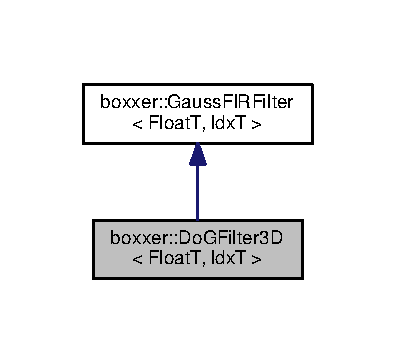
\includegraphics[width=190pt]{classboxxer_1_1DoGFilter3D__inherit__graph}
\end{center}
\end{figure}


Collaboration diagram for boxxer\+:\+:Do\+G\+Filter3D$<$ FloatT, IdxT $>$\+:\nopagebreak
\begin{figure}[H]
\begin{center}
\leavevmode
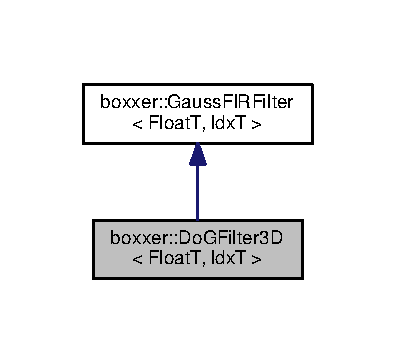
\includegraphics[width=190pt]{classboxxer_1_1DoGFilter3D__coll__graph}
\end{center}
\end{figure}
\subsubsection*{Public Types}
\begin{DoxyCompactItemize}
\item 
using \hyperlink{classboxxer_1_1DoGFilter3D_a64697cd44dcac80b42e843c05358dd26}{I\+VecT} = typename \hyperlink{classboxxer_1_1GaussFIRFilter}{Gauss\+F\+I\+R\+Filter}$<$ FloatT, IdxT $>$\+::\hyperlink{classboxxer_1_1GaussFIRFilter_a0083c8c9ab6032dd458b4dc93852c2b8}{I\+VecT}
\item 
using \hyperlink{classboxxer_1_1DoGFilter3D_aea578fd16f3044b93be02a0a634c013d}{VecT} = typename \hyperlink{classboxxer_1_1GaussFIRFilter}{Gauss\+F\+I\+R\+Filter}$<$ FloatT, IdxT $>$\+::\hyperlink{classboxxer_1_1DoGFilter3D_aea578fd16f3044b93be02a0a634c013d}{VecT}
\item 
using \hyperlink{classboxxer_1_1DoGFilter3D_ad90ef0ddf06b326066e2b62bab4e59b3}{ImageT} = arma\+::\+Cube$<$ FloatT $>$
\item 
using \hyperlink{classboxxer_1_1GaussFIRFilter_a83cf4c7f4782f69918c0e0883fff5412}{MatT} = arma\+::\+Mat$<$ FloatT $>$
\end{DoxyCompactItemize}
\subsubsection*{Public Member Functions}
\begin{DoxyCompactItemize}
\item 
\hyperlink{classboxxer_1_1DoGFilter3D_a0e754568ce65b584b0ec5840dec90d7a}{Do\+G\+Filter3D} (const \hyperlink{classboxxer_1_1GaussFIRFilter_a0083c8c9ab6032dd458b4dc93852c2b8}{I\+VecT} \&\hyperlink{classboxxer_1_1GaussFIRFilter_ac0d4e19bb2be3e8913e77283e7e4317e}{size}, const \hyperlink{classboxxer_1_1DoGFilter3D_aea578fd16f3044b93be02a0a634c013d}{VecT} \&\hyperlink{classboxxer_1_1GaussFIRFilter_a66ced06c688fd544d5f1f8be39aa2125}{sigma}, FloatT \hyperlink{classboxxer_1_1DoGFilter3D_a91ccdf9024dd9db86ba4fc9a9651b305}{sigma\+\_\+ratio})
\item 
\hyperlink{classboxxer_1_1DoGFilter3D_ab298211a58d35286158b9c88bb498a03}{Do\+G\+Filter3D} (const \hyperlink{classboxxer_1_1GaussFIRFilter_a0083c8c9ab6032dd458b4dc93852c2b8}{I\+VecT} \&\hyperlink{classboxxer_1_1GaussFIRFilter_ac0d4e19bb2be3e8913e77283e7e4317e}{size}, const \hyperlink{classboxxer_1_1DoGFilter3D_aea578fd16f3044b93be02a0a634c013d}{VecT} \&\hyperlink{classboxxer_1_1GaussFIRFilter_a66ced06c688fd544d5f1f8be39aa2125}{sigma}, FloatT \hyperlink{classboxxer_1_1DoGFilter3D_a91ccdf9024dd9db86ba4fc9a9651b305}{sigma\+\_\+ratio}, const \hyperlink{classboxxer_1_1GaussFIRFilter_a0083c8c9ab6032dd458b4dc93852c2b8}{I\+VecT} \&kernel\+\_\+hw)
\item 
void \hyperlink{classboxxer_1_1DoGFilter3D_ad28ca7638596d5113bebfdd5f131747f}{set\+\_\+kernel\+\_\+hw} (const \hyperlink{classboxxer_1_1GaussFIRFilter_a0083c8c9ab6032dd458b4dc93852c2b8}{I\+VecT} \&kernel\+\_\+half\+\_\+width)
\item 
void \hyperlink{classboxxer_1_1DoGFilter3D_a78e035961c57882c339ffbe82c92adb6}{set\+\_\+sigma\+\_\+ratio} (FloatT \hyperlink{classboxxer_1_1DoGFilter3D_a91ccdf9024dd9db86ba4fc9a9651b305}{sigma\+\_\+ratio})
\item 
\hyperlink{classboxxer_1_1DoGFilter3D_ad90ef0ddf06b326066e2b62bab4e59b3}{ImageT} \hyperlink{classboxxer_1_1DoGFilter3D_aa40d4cf7b09aac4384d30af328ea00dd}{make\+\_\+image} () const 
\item 
void \hyperlink{classboxxer_1_1DoGFilter3D_a8759b7773d369748bd69045a614f1598}{filter} (const \hyperlink{classboxxer_1_1DoGFilter3D_ad90ef0ddf06b326066e2b62bab4e59b3}{ImageT} \&im, \hyperlink{classboxxer_1_1DoGFilter3D_ad90ef0ddf06b326066e2b62bab4e59b3}{ImageT} \&out)
\item 
void \hyperlink{classboxxer_1_1DoGFilter3D_a7a30c0136590787c3a9595110f888ee3}{test\+\_\+filter} (const \hyperlink{classboxxer_1_1DoGFilter3D_ad90ef0ddf06b326066e2b62bab4e59b3}{ImageT} \&im)
\end{DoxyCompactItemize}
\subsubsection*{Static Public Member Functions}
\begin{DoxyCompactItemize}
\item 
static \hyperlink{classboxxer_1_1DoGFilter3D_aea578fd16f3044b93be02a0a634c013d}{VecT} \hyperlink{classboxxer_1_1GaussFIRFilter_a5dd6de5fe82092ec30141ab920d75dfd}{compute\+\_\+\+Gauss\+\_\+\+F\+I\+R\+\_\+kernel} (FloatT \hyperlink{classboxxer_1_1GaussFIRFilter_a66ced06c688fd544d5f1f8be39aa2125}{sigma}, IdxT \hyperlink{classboxxer_1_1GaussFIRFilter_ae17a4e137303e452a9223ba34825e0da}{hw})
\item 
static \hyperlink{classboxxer_1_1DoGFilter3D_aea578fd16f3044b93be02a0a634c013d}{VecT} \hyperlink{classboxxer_1_1GaussFIRFilter_ad6a618b47db57b570278cc57b05d8c03}{compute\+\_\+\+Lo\+G\+\_\+\+F\+I\+R\+\_\+kernel} (FloatT \hyperlink{classboxxer_1_1GaussFIRFilter_a66ced06c688fd544d5f1f8be39aa2125}{sigma}, IdxT \hyperlink{classboxxer_1_1GaussFIRFilter_ae17a4e137303e452a9223ba34825e0da}{hw})
\end{DoxyCompactItemize}
\subsubsection*{Public Attributes}
\begin{DoxyCompactItemize}
\item 
FloatT \hyperlink{classboxxer_1_1DoGFilter3D_a91ccdf9024dd9db86ba4fc9a9651b305}{sigma\+\_\+ratio}
\item 
IdxT \hyperlink{classboxxer_1_1GaussFIRFilter_ac7adcd4d8f8efee00a65262f596c8eda}{dim}
\item 
\hyperlink{classboxxer_1_1GaussFIRFilter_a0083c8c9ab6032dd458b4dc93852c2b8}{I\+VecT} \hyperlink{classboxxer_1_1GaussFIRFilter_ac0d4e19bb2be3e8913e77283e7e4317e}{size}
\item 
\hyperlink{classboxxer_1_1DoGFilter3D_aea578fd16f3044b93be02a0a634c013d}{VecT} \hyperlink{classboxxer_1_1GaussFIRFilter_a66ced06c688fd544d5f1f8be39aa2125}{sigma}
\item 
\hyperlink{classboxxer_1_1GaussFIRFilter_a0083c8c9ab6032dd458b4dc93852c2b8}{I\+VecT} \hyperlink{classboxxer_1_1GaussFIRFilter_ae17a4e137303e452a9223ba34825e0da}{hw}
\end{DoxyCompactItemize}
\subsubsection*{Static Protected Attributes}
\begin{DoxyCompactItemize}
\item 
static const IdxT \hyperlink{classboxxer_1_1GaussFIRFilter_a7f85e018f78753ee4fedf65c04b0c65a}{max\+\_\+kernel\+\_\+hw}
\item 
static const FloatT \hyperlink{classboxxer_1_1GaussFIRFilter_a72b51cd7549510735179cb9c94f5f43f}{default\+\_\+sigma\+\_\+hw\+\_\+ratio}
\end{DoxyCompactItemize}
\subsubsection*{Friends}
\begin{DoxyCompactItemize}
\item 
{\footnotesize template$<$class Float\+T\+\_\+ , class Idx\+T\+\_\+ $>$ }\\std\+::ostream \& \hyperlink{classboxxer_1_1DoGFilter3D_a3e7ff88dad2f821551e56939779d24ba}{operator$<$$<$} (std\+::ostream \&out, const \hyperlink{classboxxer_1_1GaussFilter3D}{Gauss\+Filter3D}$<$ Float\+T\+\_\+, Idx\+T\+\_\+ $>$ \&filt)
\end{DoxyCompactItemize}


\subsubsection{Detailed Description}
\subsubsection*{template$<$class FloatT = float, class IdxT = uint32\+\_\+t$>$\\*
class boxxer\+::\+Do\+G\+Filter3\+D$<$ Float\+T, Idx\+T $>$}



Definition at line 150 of file Gauss\+Filter.\+h.



\subsubsection{Member Typedef Documentation}
\index{boxxer\+::\+Do\+G\+Filter3D@{boxxer\+::\+Do\+G\+Filter3D}!ImageT@{ImageT}}
\index{ImageT@{ImageT}!boxxer\+::\+Do\+G\+Filter3D@{boxxer\+::\+Do\+G\+Filter3D}}
\paragraph[{\texorpdfstring{ImageT}{ImageT}}]{\setlength{\rightskip}{0pt plus 5cm}template$<$class FloatT  = float, class IdxT  = uint32\+\_\+t$>$ using {\bf boxxer\+::\+Do\+G\+Filter3D}$<$ FloatT, IdxT $>$\+::{\bf ImageT} =  arma\+::\+Cube$<$FloatT$>$}\hypertarget{classboxxer_1_1DoGFilter3D_ad90ef0ddf06b326066e2b62bab4e59b3}{}\label{classboxxer_1_1DoGFilter3D_ad90ef0ddf06b326066e2b62bab4e59b3}


Definition at line 155 of file Gauss\+Filter.\+h.

\index{boxxer\+::\+Do\+G\+Filter3D@{boxxer\+::\+Do\+G\+Filter3D}!I\+VecT@{I\+VecT}}
\index{I\+VecT@{I\+VecT}!boxxer\+::\+Do\+G\+Filter3D@{boxxer\+::\+Do\+G\+Filter3D}}
\paragraph[{\texorpdfstring{I\+VecT}{IVecT}}]{\setlength{\rightskip}{0pt plus 5cm}template$<$class FloatT  = float, class IdxT  = uint32\+\_\+t$>$ using {\bf boxxer\+::\+Do\+G\+Filter3D}$<$ FloatT, IdxT $>$\+::{\bf I\+VecT} =  typename {\bf Gauss\+F\+I\+R\+Filter}$<$FloatT,IdxT$>$\+::{\bf I\+VecT}}\hypertarget{classboxxer_1_1DoGFilter3D_a64697cd44dcac80b42e843c05358dd26}{}\label{classboxxer_1_1DoGFilter3D_a64697cd44dcac80b42e843c05358dd26}


Definition at line 153 of file Gauss\+Filter.\+h.

\index{boxxer\+::\+Do\+G\+Filter3D@{boxxer\+::\+Do\+G\+Filter3D}!MatT@{MatT}}
\index{MatT@{MatT}!boxxer\+::\+Do\+G\+Filter3D@{boxxer\+::\+Do\+G\+Filter3D}}
\paragraph[{\texorpdfstring{MatT}{MatT}}]{\setlength{\rightskip}{0pt plus 5cm}template$<$class FloatT = float, class IdxT = uint32\+\_\+t$>$ using {\bf boxxer\+::\+Gauss\+F\+I\+R\+Filter}$<$ FloatT, IdxT $>$\+::{\bf MatT} =  arma\+::\+Mat$<$FloatT$>$\hspace{0.3cm}{\ttfamily [inherited]}}\hypertarget{classboxxer_1_1GaussFIRFilter_a83cf4c7f4782f69918c0e0883fff5412}{}\label{classboxxer_1_1GaussFIRFilter_a83cf4c7f4782f69918c0e0883fff5412}


Definition at line 26 of file Gauss\+Filter.\+h.

\index{boxxer\+::\+Do\+G\+Filter3D@{boxxer\+::\+Do\+G\+Filter3D}!VecT@{VecT}}
\index{VecT@{VecT}!boxxer\+::\+Do\+G\+Filter3D@{boxxer\+::\+Do\+G\+Filter3D}}
\paragraph[{\texorpdfstring{VecT}{VecT}}]{\setlength{\rightskip}{0pt plus 5cm}template$<$class FloatT  = float, class IdxT  = uint32\+\_\+t$>$ using {\bf boxxer\+::\+Do\+G\+Filter3D}$<$ FloatT, IdxT $>$\+::{\bf VecT} =  typename {\bf Gauss\+F\+I\+R\+Filter}$<$FloatT,IdxT$>$\+::{\bf VecT}}\hypertarget{classboxxer_1_1DoGFilter3D_aea578fd16f3044b93be02a0a634c013d}{}\label{classboxxer_1_1DoGFilter3D_aea578fd16f3044b93be02a0a634c013d}


Definition at line 154 of file Gauss\+Filter.\+h.



\subsubsection{Constructor \& Destructor Documentation}
\index{boxxer\+::\+Do\+G\+Filter3D@{boxxer\+::\+Do\+G\+Filter3D}!Do\+G\+Filter3D@{Do\+G\+Filter3D}}
\index{Do\+G\+Filter3D@{Do\+G\+Filter3D}!boxxer\+::\+Do\+G\+Filter3D@{boxxer\+::\+Do\+G\+Filter3D}}
\paragraph[{\texorpdfstring{Do\+G\+Filter3\+D(const I\+Vec\+T \&size, const Vec\+T \&sigma, Float\+T sigma\+\_\+ratio)}{DoGFilter3D(const IVecT &size, const VecT &sigma, FloatT sigma_ratio)}}]{\setlength{\rightskip}{0pt plus 5cm}template$<$class FloatT  = float, class IdxT  = uint32\+\_\+t$>$ {\bf boxxer\+::\+Do\+G\+Filter3D}$<$ FloatT, IdxT $>$\+::{\bf Do\+G\+Filter3D} (
\begin{DoxyParamCaption}
\item[{const {\bf I\+VecT} \&}]{size, }
\item[{const {\bf VecT} \&}]{sigma, }
\item[{FloatT}]{sigma\+\_\+ratio}
\end{DoxyParamCaption}
)}\hypertarget{classboxxer_1_1DoGFilter3D_a0e754568ce65b584b0ec5840dec90d7a}{}\label{classboxxer_1_1DoGFilter3D_a0e754568ce65b584b0ec5840dec90d7a}
\index{boxxer\+::\+Do\+G\+Filter3D@{boxxer\+::\+Do\+G\+Filter3D}!Do\+G\+Filter3D@{Do\+G\+Filter3D}}
\index{Do\+G\+Filter3D@{Do\+G\+Filter3D}!boxxer\+::\+Do\+G\+Filter3D@{boxxer\+::\+Do\+G\+Filter3D}}
\paragraph[{\texorpdfstring{Do\+G\+Filter3\+D(const I\+Vec\+T \&size, const Vec\+T \&sigma, Float\+T sigma\+\_\+ratio, const I\+Vec\+T \&kernel\+\_\+hw)}{DoGFilter3D(const IVecT &size, const VecT &sigma, FloatT sigma_ratio, const IVecT &kernel_hw)}}]{\setlength{\rightskip}{0pt plus 5cm}template$<$class FloatT  = float, class IdxT  = uint32\+\_\+t$>$ {\bf boxxer\+::\+Do\+G\+Filter3D}$<$ FloatT, IdxT $>$\+::{\bf Do\+G\+Filter3D} (
\begin{DoxyParamCaption}
\item[{const {\bf I\+VecT} \&}]{size, }
\item[{const {\bf VecT} \&}]{sigma, }
\item[{FloatT}]{sigma\+\_\+ratio, }
\item[{const {\bf I\+VecT} \&}]{kernel\+\_\+hw}
\end{DoxyParamCaption}
)}\hypertarget{classboxxer_1_1DoGFilter3D_ab298211a58d35286158b9c88bb498a03}{}\label{classboxxer_1_1DoGFilter3D_ab298211a58d35286158b9c88bb498a03}


\subsubsection{Member Function Documentation}
\index{boxxer\+::\+Do\+G\+Filter3D@{boxxer\+::\+Do\+G\+Filter3D}!compute\+\_\+\+Gauss\+\_\+\+F\+I\+R\+\_\+kernel@{compute\+\_\+\+Gauss\+\_\+\+F\+I\+R\+\_\+kernel}}
\index{compute\+\_\+\+Gauss\+\_\+\+F\+I\+R\+\_\+kernel@{compute\+\_\+\+Gauss\+\_\+\+F\+I\+R\+\_\+kernel}!boxxer\+::\+Do\+G\+Filter3D@{boxxer\+::\+Do\+G\+Filter3D}}
\paragraph[{\texorpdfstring{compute\+\_\+\+Gauss\+\_\+\+F\+I\+R\+\_\+kernel(\+Float\+T sigma, Idx\+T hw)}{compute_Gauss_FIR_kernel(FloatT sigma, IdxT hw)}}]{\setlength{\rightskip}{0pt plus 5cm}template$<$class FloatT = float, class IdxT = uint32\+\_\+t$>$ static {\bf VecT} {\bf boxxer\+::\+Gauss\+F\+I\+R\+Filter}$<$ FloatT, IdxT $>$\+::compute\+\_\+\+Gauss\+\_\+\+F\+I\+R\+\_\+kernel (
\begin{DoxyParamCaption}
\item[{FloatT}]{sigma, }
\item[{IdxT}]{hw}
\end{DoxyParamCaption}
)\hspace{0.3cm}{\ttfamily [static]}, {\ttfamily [inherited]}}\hypertarget{classboxxer_1_1GaussFIRFilter_a5dd6de5fe82092ec30141ab920d75dfd}{}\label{classboxxer_1_1GaussFIRFilter_a5dd6de5fe82092ec30141ab920d75dfd}
\index{boxxer\+::\+Do\+G\+Filter3D@{boxxer\+::\+Do\+G\+Filter3D}!compute\+\_\+\+Lo\+G\+\_\+\+F\+I\+R\+\_\+kernel@{compute\+\_\+\+Lo\+G\+\_\+\+F\+I\+R\+\_\+kernel}}
\index{compute\+\_\+\+Lo\+G\+\_\+\+F\+I\+R\+\_\+kernel@{compute\+\_\+\+Lo\+G\+\_\+\+F\+I\+R\+\_\+kernel}!boxxer\+::\+Do\+G\+Filter3D@{boxxer\+::\+Do\+G\+Filter3D}}
\paragraph[{\texorpdfstring{compute\+\_\+\+Lo\+G\+\_\+\+F\+I\+R\+\_\+kernel(\+Float\+T sigma, Idx\+T hw)}{compute_LoG_FIR_kernel(FloatT sigma, IdxT hw)}}]{\setlength{\rightskip}{0pt plus 5cm}template$<$class FloatT = float, class IdxT = uint32\+\_\+t$>$ static {\bf VecT} {\bf boxxer\+::\+Gauss\+F\+I\+R\+Filter}$<$ FloatT, IdxT $>$\+::compute\+\_\+\+Lo\+G\+\_\+\+F\+I\+R\+\_\+kernel (
\begin{DoxyParamCaption}
\item[{FloatT}]{sigma, }
\item[{IdxT}]{hw}
\end{DoxyParamCaption}
)\hspace{0.3cm}{\ttfamily [static]}, {\ttfamily [inherited]}}\hypertarget{classboxxer_1_1GaussFIRFilter_ad6a618b47db57b570278cc57b05d8c03}{}\label{classboxxer_1_1GaussFIRFilter_ad6a618b47db57b570278cc57b05d8c03}
\index{boxxer\+::\+Do\+G\+Filter3D@{boxxer\+::\+Do\+G\+Filter3D}!filter@{filter}}
\index{filter@{filter}!boxxer\+::\+Do\+G\+Filter3D@{boxxer\+::\+Do\+G\+Filter3D}}
\paragraph[{\texorpdfstring{filter(const Image\+T \&im, Image\+T \&out)}{filter(const ImageT &im, ImageT &out)}}]{\setlength{\rightskip}{0pt plus 5cm}template$<$class FloatT  = float, class IdxT  = uint32\+\_\+t$>$ void {\bf boxxer\+::\+Do\+G\+Filter3D}$<$ FloatT, IdxT $>$\+::filter (
\begin{DoxyParamCaption}
\item[{const {\bf ImageT} \&}]{im, }
\item[{{\bf ImageT} \&}]{out}
\end{DoxyParamCaption}
)}\hypertarget{classboxxer_1_1DoGFilter3D_a8759b7773d369748bd69045a614f1598}{}\label{classboxxer_1_1DoGFilter3D_a8759b7773d369748bd69045a614f1598}
\index{boxxer\+::\+Do\+G\+Filter3D@{boxxer\+::\+Do\+G\+Filter3D}!make\+\_\+image@{make\+\_\+image}}
\index{make\+\_\+image@{make\+\_\+image}!boxxer\+::\+Do\+G\+Filter3D@{boxxer\+::\+Do\+G\+Filter3D}}
\paragraph[{\texorpdfstring{make\+\_\+image() const }{make_image() const }}]{\setlength{\rightskip}{0pt plus 5cm}template$<$class FloatT  = float, class IdxT  = uint32\+\_\+t$>$ {\bf ImageT} {\bf boxxer\+::\+Do\+G\+Filter3D}$<$ FloatT, IdxT $>$\+::make\+\_\+image (
\begin{DoxyParamCaption}
{}
\end{DoxyParamCaption}
) const\hspace{0.3cm}{\ttfamily [inline]}}\hypertarget{classboxxer_1_1DoGFilter3D_aa40d4cf7b09aac4384d30af328ea00dd}{}\label{classboxxer_1_1DoGFilter3D_aa40d4cf7b09aac4384d30af328ea00dd}


Definition at line 163 of file Gauss\+Filter.\+h.



References boxxer\+::\+Gauss\+F\+I\+R\+Filter$<$ Float\+T, Idx\+T $>$\+::size.

\index{boxxer\+::\+Do\+G\+Filter3D@{boxxer\+::\+Do\+G\+Filter3D}!set\+\_\+kernel\+\_\+hw@{set\+\_\+kernel\+\_\+hw}}
\index{set\+\_\+kernel\+\_\+hw@{set\+\_\+kernel\+\_\+hw}!boxxer\+::\+Do\+G\+Filter3D@{boxxer\+::\+Do\+G\+Filter3D}}
\paragraph[{\texorpdfstring{set\+\_\+kernel\+\_\+hw(const I\+Vec\+T \&kernel\+\_\+half\+\_\+width)}{set_kernel_hw(const IVecT &kernel_half_width)}}]{\setlength{\rightskip}{0pt plus 5cm}template$<$class FloatT  = float, class IdxT  = uint32\+\_\+t$>$ void {\bf boxxer\+::\+Do\+G\+Filter3D}$<$ FloatT, IdxT $>$\+::set\+\_\+kernel\+\_\+hw (
\begin{DoxyParamCaption}
\item[{const {\bf I\+VecT} \&}]{kernel\+\_\+half\+\_\+width}
\end{DoxyParamCaption}
)\hspace{0.3cm}{\ttfamily [virtual]}}\hypertarget{classboxxer_1_1DoGFilter3D_ad28ca7638596d5113bebfdd5f131747f}{}\label{classboxxer_1_1DoGFilter3D_ad28ca7638596d5113bebfdd5f131747f}


Implements \hyperlink{classboxxer_1_1GaussFIRFilter_a7ada113680b67f052d11afe346ddf8bc}{boxxer\+::\+Gauss\+F\+I\+R\+Filter$<$ Float\+T, Idx\+T $>$}.

\index{boxxer\+::\+Do\+G\+Filter3D@{boxxer\+::\+Do\+G\+Filter3D}!set\+\_\+sigma\+\_\+ratio@{set\+\_\+sigma\+\_\+ratio}}
\index{set\+\_\+sigma\+\_\+ratio@{set\+\_\+sigma\+\_\+ratio}!boxxer\+::\+Do\+G\+Filter3D@{boxxer\+::\+Do\+G\+Filter3D}}
\paragraph[{\texorpdfstring{set\+\_\+sigma\+\_\+ratio(\+Float\+T sigma\+\_\+ratio)}{set_sigma_ratio(FloatT sigma_ratio)}}]{\setlength{\rightskip}{0pt plus 5cm}template$<$class FloatT  = float, class IdxT  = uint32\+\_\+t$>$ void {\bf boxxer\+::\+Do\+G\+Filter3D}$<$ FloatT, IdxT $>$\+::set\+\_\+sigma\+\_\+ratio (
\begin{DoxyParamCaption}
\item[{FloatT}]{sigma\+\_\+ratio}
\end{DoxyParamCaption}
)}\hypertarget{classboxxer_1_1DoGFilter3D_a78e035961c57882c339ffbe82c92adb6}{}\label{classboxxer_1_1DoGFilter3D_a78e035961c57882c339ffbe82c92adb6}
\index{boxxer\+::\+Do\+G\+Filter3D@{boxxer\+::\+Do\+G\+Filter3D}!test\+\_\+filter@{test\+\_\+filter}}
\index{test\+\_\+filter@{test\+\_\+filter}!boxxer\+::\+Do\+G\+Filter3D@{boxxer\+::\+Do\+G\+Filter3D}}
\paragraph[{\texorpdfstring{test\+\_\+filter(const Image\+T \&im)}{test_filter(const ImageT &im)}}]{\setlength{\rightskip}{0pt plus 5cm}template$<$class FloatT  = float, class IdxT  = uint32\+\_\+t$>$ void {\bf boxxer\+::\+Do\+G\+Filter3D}$<$ FloatT, IdxT $>$\+::test\+\_\+filter (
\begin{DoxyParamCaption}
\item[{const {\bf ImageT} \&}]{im}
\end{DoxyParamCaption}
)}\hypertarget{classboxxer_1_1DoGFilter3D_a7a30c0136590787c3a9595110f888ee3}{}\label{classboxxer_1_1DoGFilter3D_a7a30c0136590787c3a9595110f888ee3}


\subsubsection{Friends And Related Function Documentation}
\index{boxxer\+::\+Do\+G\+Filter3D@{boxxer\+::\+Do\+G\+Filter3D}!operator$<$$<$@{operator$<$$<$}}
\index{operator$<$$<$@{operator$<$$<$}!boxxer\+::\+Do\+G\+Filter3D@{boxxer\+::\+Do\+G\+Filter3D}}
\paragraph[{\texorpdfstring{operator$<$$<$}{operator<<}}]{\setlength{\rightskip}{0pt plus 5cm}template$<$class FloatT  = float, class IdxT  = uint32\+\_\+t$>$ template$<$class Float\+T\+\_\+ , class Idx\+T\+\_\+ $>$ std\+::ostream\& operator$<$$<$ (
\begin{DoxyParamCaption}
\item[{std\+::ostream \&}]{out, }
\item[{const {\bf Gauss\+Filter3D}$<$ Float\+T\+\_\+, Idx\+T\+\_\+ $>$ \&}]{filt}
\end{DoxyParamCaption}
)\hspace{0.3cm}{\ttfamily [friend]}}\hypertarget{classboxxer_1_1DoGFilter3D_a3e7ff88dad2f821551e56939779d24ba}{}\label{classboxxer_1_1DoGFilter3D_a3e7ff88dad2f821551e56939779d24ba}


\subsubsection{Member Data Documentation}
\index{boxxer\+::\+Do\+G\+Filter3D@{boxxer\+::\+Do\+G\+Filter3D}!default\+\_\+sigma\+\_\+hw\+\_\+ratio@{default\+\_\+sigma\+\_\+hw\+\_\+ratio}}
\index{default\+\_\+sigma\+\_\+hw\+\_\+ratio@{default\+\_\+sigma\+\_\+hw\+\_\+ratio}!boxxer\+::\+Do\+G\+Filter3D@{boxxer\+::\+Do\+G\+Filter3D}}
\paragraph[{\texorpdfstring{default\+\_\+sigma\+\_\+hw\+\_\+ratio}{default_sigma_hw_ratio}}]{\setlength{\rightskip}{0pt plus 5cm}template$<$class FloatT = float, class IdxT = uint32\+\_\+t$>$ const FloatT {\bf boxxer\+::\+Gauss\+F\+I\+R\+Filter}$<$ FloatT, IdxT $>$\+::default\+\_\+sigma\+\_\+hw\+\_\+ratio\hspace{0.3cm}{\ttfamily [static]}, {\ttfamily [protected]}, {\ttfamily [inherited]}}\hypertarget{classboxxer_1_1GaussFIRFilter_a72b51cd7549510735179cb9c94f5f43f}{}\label{classboxxer_1_1GaussFIRFilter_a72b51cd7549510735179cb9c94f5f43f}


Definition at line 41 of file Gauss\+Filter.\+h.

\index{boxxer\+::\+Do\+G\+Filter3D@{boxxer\+::\+Do\+G\+Filter3D}!dim@{dim}}
\index{dim@{dim}!boxxer\+::\+Do\+G\+Filter3D@{boxxer\+::\+Do\+G\+Filter3D}}
\paragraph[{\texorpdfstring{dim}{dim}}]{\setlength{\rightskip}{0pt plus 5cm}template$<$class FloatT = float, class IdxT = uint32\+\_\+t$>$ IdxT {\bf boxxer\+::\+Gauss\+F\+I\+R\+Filter}$<$ FloatT, IdxT $>$\+::dim\hspace{0.3cm}{\ttfamily [inherited]}}\hypertarget{classboxxer_1_1GaussFIRFilter_ac7adcd4d8f8efee00a65262f596c8eda}{}\label{classboxxer_1_1GaussFIRFilter_ac7adcd4d8f8efee00a65262f596c8eda}


Definition at line 28 of file Gauss\+Filter.\+h.

\index{boxxer\+::\+Do\+G\+Filter3D@{boxxer\+::\+Do\+G\+Filter3D}!hw@{hw}}
\index{hw@{hw}!boxxer\+::\+Do\+G\+Filter3D@{boxxer\+::\+Do\+G\+Filter3D}}
\paragraph[{\texorpdfstring{hw}{hw}}]{\setlength{\rightskip}{0pt plus 5cm}template$<$class FloatT = float, class IdxT = uint32\+\_\+t$>$ {\bf I\+VecT} {\bf boxxer\+::\+Gauss\+F\+I\+R\+Filter}$<$ FloatT, IdxT $>$\+::hw\hspace{0.3cm}{\ttfamily [inherited]}}\hypertarget{classboxxer_1_1GaussFIRFilter_ae17a4e137303e452a9223ba34825e0da}{}\label{classboxxer_1_1GaussFIRFilter_ae17a4e137303e452a9223ba34825e0da}


Definition at line 31 of file Gauss\+Filter.\+h.

\index{boxxer\+::\+Do\+G\+Filter3D@{boxxer\+::\+Do\+G\+Filter3D}!max\+\_\+kernel\+\_\+hw@{max\+\_\+kernel\+\_\+hw}}
\index{max\+\_\+kernel\+\_\+hw@{max\+\_\+kernel\+\_\+hw}!boxxer\+::\+Do\+G\+Filter3D@{boxxer\+::\+Do\+G\+Filter3D}}
\paragraph[{\texorpdfstring{max\+\_\+kernel\+\_\+hw}{max_kernel_hw}}]{\setlength{\rightskip}{0pt plus 5cm}template$<$class FloatT = float, class IdxT = uint32\+\_\+t$>$ const IdxT {\bf boxxer\+::\+Gauss\+F\+I\+R\+Filter}$<$ FloatT, IdxT $>$\+::max\+\_\+kernel\+\_\+hw\hspace{0.3cm}{\ttfamily [static]}, {\ttfamily [protected]}, {\ttfamily [inherited]}}\hypertarget{classboxxer_1_1GaussFIRFilter_a7f85e018f78753ee4fedf65c04b0c65a}{}\label{classboxxer_1_1GaussFIRFilter_a7f85e018f78753ee4fedf65c04b0c65a}


Definition at line 40 of file Gauss\+Filter.\+h.

\index{boxxer\+::\+Do\+G\+Filter3D@{boxxer\+::\+Do\+G\+Filter3D}!sigma@{sigma}}
\index{sigma@{sigma}!boxxer\+::\+Do\+G\+Filter3D@{boxxer\+::\+Do\+G\+Filter3D}}
\paragraph[{\texorpdfstring{sigma}{sigma}}]{\setlength{\rightskip}{0pt plus 5cm}template$<$class FloatT = float, class IdxT = uint32\+\_\+t$>$ {\bf VecT} {\bf boxxer\+::\+Gauss\+F\+I\+R\+Filter}$<$ FloatT, IdxT $>$\+::sigma\hspace{0.3cm}{\ttfamily [inherited]}}\hypertarget{classboxxer_1_1GaussFIRFilter_a66ced06c688fd544d5f1f8be39aa2125}{}\label{classboxxer_1_1GaussFIRFilter_a66ced06c688fd544d5f1f8be39aa2125}


Definition at line 30 of file Gauss\+Filter.\+h.

\index{boxxer\+::\+Do\+G\+Filter3D@{boxxer\+::\+Do\+G\+Filter3D}!sigma\+\_\+ratio@{sigma\+\_\+ratio}}
\index{sigma\+\_\+ratio@{sigma\+\_\+ratio}!boxxer\+::\+Do\+G\+Filter3D@{boxxer\+::\+Do\+G\+Filter3D}}
\paragraph[{\texorpdfstring{sigma\+\_\+ratio}{sigma_ratio}}]{\setlength{\rightskip}{0pt plus 5cm}template$<$class FloatT  = float, class IdxT  = uint32\+\_\+t$>$ FloatT {\bf boxxer\+::\+Do\+G\+Filter3D}$<$ FloatT, IdxT $>$\+::sigma\+\_\+ratio}\hypertarget{classboxxer_1_1DoGFilter3D_a91ccdf9024dd9db86ba4fc9a9651b305}{}\label{classboxxer_1_1DoGFilter3D_a91ccdf9024dd9db86ba4fc9a9651b305}


Definition at line 157 of file Gauss\+Filter.\+h.

\index{boxxer\+::\+Do\+G\+Filter3D@{boxxer\+::\+Do\+G\+Filter3D}!size@{size}}
\index{size@{size}!boxxer\+::\+Do\+G\+Filter3D@{boxxer\+::\+Do\+G\+Filter3D}}
\paragraph[{\texorpdfstring{size}{size}}]{\setlength{\rightskip}{0pt plus 5cm}template$<$class FloatT = float, class IdxT = uint32\+\_\+t$>$ {\bf I\+VecT} {\bf boxxer\+::\+Gauss\+F\+I\+R\+Filter}$<$ FloatT, IdxT $>$\+::size\hspace{0.3cm}{\ttfamily [inherited]}}\hypertarget{classboxxer_1_1GaussFIRFilter_ac0d4e19bb2be3e8913e77283e7e4317e}{}\label{classboxxer_1_1GaussFIRFilter_ac0d4e19bb2be3e8913e77283e7e4317e}


Definition at line 29 of file Gauss\+Filter.\+h.



Referenced by boxxer\+::\+Gauss\+Filter2\+D$<$ Float\+T, Idx\+T $>$\+::make\+\_\+image(), boxxer\+::\+Do\+G\+Filter2\+D$<$ Float\+T, Idx\+T $>$\+::make\+\_\+image(), boxxer\+::\+Lo\+G\+Filter2\+D$<$ Float\+T, Idx\+T $>$\+::make\+\_\+image(), boxxer\+::\+Gauss\+Filter3\+D$<$ Float\+T, Idx\+T $>$\+::make\+\_\+image(), boxxer\+::\+Do\+G\+Filter3\+D$<$ Float\+T, Idx\+T $>$\+::make\+\_\+image(), and boxxer\+::\+Lo\+G\+Filter3\+D$<$ Float\+T, Idx\+T $>$\+::make\+\_\+image().



The documentation for this class was generated from the following file\+:\begin{DoxyCompactItemize}
\item 
\hyperlink{GaussFilter_8h}{Gauss\+Filter.\+h}\end{DoxyCompactItemize}

\hypertarget{classboxxer_1_1GaussFilter2D}{}\subsection{boxxer\+:\+:Gauss\+Filter2D$<$ FloatT, IdxT $>$ Class Template Reference}
\label{classboxxer_1_1GaussFilter2D}\index{boxxer\+::\+Gauss\+Filter2\+D$<$ Float\+T, Idx\+T $>$@{boxxer\+::\+Gauss\+Filter2\+D$<$ Float\+T, Idx\+T $>$}}


{\ttfamily \#include $<$/home/travis/build/markjolah/\+Boxxer/include/\+Boxxer/\+Gauss\+Filter.\+h$>$}



Inheritance diagram for boxxer\+:\+:Gauss\+Filter2D$<$ FloatT, IdxT $>$\+:\nopagebreak
\begin{figure}[H]
\begin{center}
\leavevmode
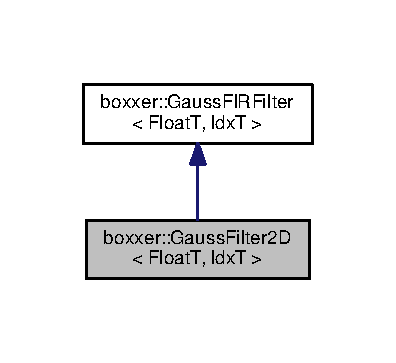
\includegraphics[width=190pt]{classboxxer_1_1GaussFilter2D__inherit__graph}
\end{center}
\end{figure}


Collaboration diagram for boxxer\+:\+:Gauss\+Filter2D$<$ FloatT, IdxT $>$\+:\nopagebreak
\begin{figure}[H]
\begin{center}
\leavevmode
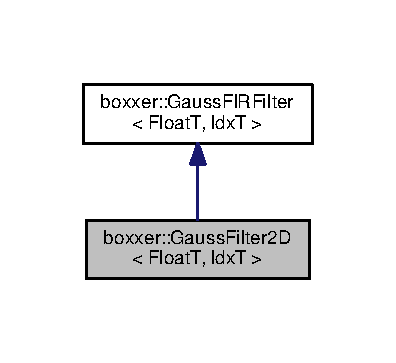
\includegraphics[width=190pt]{classboxxer_1_1GaussFilter2D__coll__graph}
\end{center}
\end{figure}
\subsubsection*{Public Types}
\begin{DoxyCompactItemize}
\item 
using \hyperlink{classboxxer_1_1GaussFilter2D_a887e8b8aab3bf93d17be4335512e3dfe}{I\+VecT} = typename \hyperlink{classboxxer_1_1GaussFIRFilter}{Gauss\+F\+I\+R\+Filter}$<$ FloatT, IdxT $>$\+::\hyperlink{classboxxer_1_1GaussFIRFilter_a0083c8c9ab6032dd458b4dc93852c2b8}{I\+VecT}
\item 
using \hyperlink{classboxxer_1_1GaussFilter2D_a43b1093b492791f308036e6729cf765e}{VecT} = typename \hyperlink{classboxxer_1_1GaussFIRFilter}{Gauss\+F\+I\+R\+Filter}$<$ FloatT, IdxT $>$\+::\hyperlink{classboxxer_1_1GaussFilter2D_a43b1093b492791f308036e6729cf765e}{VecT}
\item 
using \hyperlink{classboxxer_1_1GaussFilter2D_ae23c8679409815813d371743d9645565}{ImageT} = arma\+::\+Mat$<$ FloatT $>$
\item 
using \hyperlink{classboxxer_1_1GaussFIRFilter_a83cf4c7f4782f69918c0e0883fff5412}{MatT} = arma\+::\+Mat$<$ FloatT $>$
\end{DoxyCompactItemize}
\subsubsection*{Public Member Functions}
\begin{DoxyCompactItemize}
\item 
\hyperlink{classboxxer_1_1GaussFilter2D_a131316827df77a205e23788431778b75}{Gauss\+Filter2D} (const \hyperlink{classboxxer_1_1GaussFIRFilter_a0083c8c9ab6032dd458b4dc93852c2b8}{I\+VecT} \&\hyperlink{classboxxer_1_1GaussFIRFilter_ac0d4e19bb2be3e8913e77283e7e4317e}{size}, const \hyperlink{classboxxer_1_1GaussFilter2D_a43b1093b492791f308036e6729cf765e}{VecT} \&\hyperlink{classboxxer_1_1GaussFIRFilter_a66ced06c688fd544d5f1f8be39aa2125}{sigma})
\item 
\hyperlink{classboxxer_1_1GaussFilter2D_a37a89756c10a34ed6a5098520f8d7747}{Gauss\+Filter2D} (const \hyperlink{classboxxer_1_1GaussFIRFilter_a0083c8c9ab6032dd458b4dc93852c2b8}{I\+VecT} \&\hyperlink{classboxxer_1_1GaussFIRFilter_ac0d4e19bb2be3e8913e77283e7e4317e}{size}, const \hyperlink{classboxxer_1_1GaussFilter2D_a43b1093b492791f308036e6729cf765e}{VecT} \&\hyperlink{classboxxer_1_1GaussFIRFilter_a66ced06c688fd544d5f1f8be39aa2125}{sigma}, const \hyperlink{classboxxer_1_1GaussFIRFilter_a0083c8c9ab6032dd458b4dc93852c2b8}{I\+VecT} \&kernel\+\_\+hw)
\item 
void \hyperlink{classboxxer_1_1GaussFilter2D_a9829d0790d5d1b0931a09cb3e9afe07f}{set\+\_\+kernel\+\_\+hw} (const \hyperlink{classboxxer_1_1GaussFIRFilter_a0083c8c9ab6032dd458b4dc93852c2b8}{I\+VecT} \&kernel\+\_\+half\+\_\+width)
\item 
\hyperlink{classboxxer_1_1GaussFilter2D_ae23c8679409815813d371743d9645565}{ImageT} \hyperlink{classboxxer_1_1GaussFilter2D_a00c1d3d16f47a9293b79202d187938b8}{make\+\_\+image} () const 
\item 
void \hyperlink{classboxxer_1_1GaussFilter2D_aac5d338e756dcf5016653d93f6d05bd3}{filter} (const \hyperlink{classboxxer_1_1GaussFilter2D_ae23c8679409815813d371743d9645565}{ImageT} \&im, \hyperlink{classboxxer_1_1GaussFilter2D_ae23c8679409815813d371743d9645565}{ImageT} \&out)
\item 
void \hyperlink{classboxxer_1_1GaussFilter2D_a9bb46c4fc45f4658387e309253d4f12a}{test\+\_\+filter} (const \hyperlink{classboxxer_1_1GaussFilter2D_ae23c8679409815813d371743d9645565}{ImageT} \&im)
\end{DoxyCompactItemize}
\subsubsection*{Static Public Member Functions}
\begin{DoxyCompactItemize}
\item 
static \hyperlink{classboxxer_1_1GaussFilter2D_a43b1093b492791f308036e6729cf765e}{VecT} \hyperlink{classboxxer_1_1GaussFIRFilter_a5dd6de5fe82092ec30141ab920d75dfd}{compute\+\_\+\+Gauss\+\_\+\+F\+I\+R\+\_\+kernel} (FloatT \hyperlink{classboxxer_1_1GaussFIRFilter_a66ced06c688fd544d5f1f8be39aa2125}{sigma}, IdxT \hyperlink{classboxxer_1_1GaussFIRFilter_ae17a4e137303e452a9223ba34825e0da}{hw})
\item 
static \hyperlink{classboxxer_1_1GaussFilter2D_a43b1093b492791f308036e6729cf765e}{VecT} \hyperlink{classboxxer_1_1GaussFIRFilter_ad6a618b47db57b570278cc57b05d8c03}{compute\+\_\+\+Lo\+G\+\_\+\+F\+I\+R\+\_\+kernel} (FloatT \hyperlink{classboxxer_1_1GaussFIRFilter_a66ced06c688fd544d5f1f8be39aa2125}{sigma}, IdxT \hyperlink{classboxxer_1_1GaussFIRFilter_ae17a4e137303e452a9223ba34825e0da}{hw})
\end{DoxyCompactItemize}
\subsubsection*{Public Attributes}
\begin{DoxyCompactItemize}
\item 
IdxT \hyperlink{classboxxer_1_1GaussFIRFilter_ac7adcd4d8f8efee00a65262f596c8eda}{dim}
\item 
\hyperlink{classboxxer_1_1GaussFIRFilter_a0083c8c9ab6032dd458b4dc93852c2b8}{I\+VecT} \hyperlink{classboxxer_1_1GaussFIRFilter_ac0d4e19bb2be3e8913e77283e7e4317e}{size}
\item 
\hyperlink{classboxxer_1_1GaussFilter2D_a43b1093b492791f308036e6729cf765e}{VecT} \hyperlink{classboxxer_1_1GaussFIRFilter_a66ced06c688fd544d5f1f8be39aa2125}{sigma}
\item 
\hyperlink{classboxxer_1_1GaussFIRFilter_a0083c8c9ab6032dd458b4dc93852c2b8}{I\+VecT} \hyperlink{classboxxer_1_1GaussFIRFilter_ae17a4e137303e452a9223ba34825e0da}{hw}
\end{DoxyCompactItemize}
\subsubsection*{Static Protected Attributes}
\begin{DoxyCompactItemize}
\item 
static const IdxT \hyperlink{classboxxer_1_1GaussFIRFilter_a7f85e018f78753ee4fedf65c04b0c65a}{max\+\_\+kernel\+\_\+hw}
\item 
static const FloatT \hyperlink{classboxxer_1_1GaussFIRFilter_a72b51cd7549510735179cb9c94f5f43f}{default\+\_\+sigma\+\_\+hw\+\_\+ratio}
\end{DoxyCompactItemize}
\subsubsection*{Friends}
\begin{DoxyCompactItemize}
\item 
{\footnotesize template$<$class Float\+T\+\_\+ , class Idx\+T\+\_\+ $>$ }\\std\+::ostream \& \hyperlink{classboxxer_1_1GaussFilter2D_abb41be01824fced1029c5fc686a80d98}{operator$<$$<$} (std\+::ostream \&out, const \hyperlink{classboxxer_1_1GaussFilter2D}{Gauss\+Filter2D}$<$ Float\+T\+\_\+, Idx\+T\+\_\+ $>$ \&filt)
\end{DoxyCompactItemize}


\subsubsection{Detailed Description}
\subsubsection*{template$<$class FloatT = float, class IdxT = uint32\+\_\+t$>$\\*
class boxxer\+::\+Gauss\+Filter2\+D$<$ Float\+T, Idx\+T $>$}

2D Filters 

Definition at line 47 of file Gauss\+Filter.\+h.



\subsubsection{Member Typedef Documentation}
\index{boxxer\+::\+Gauss\+Filter2D@{boxxer\+::\+Gauss\+Filter2D}!ImageT@{ImageT}}
\index{ImageT@{ImageT}!boxxer\+::\+Gauss\+Filter2D@{boxxer\+::\+Gauss\+Filter2D}}
\paragraph[{\texorpdfstring{ImageT}{ImageT}}]{\setlength{\rightskip}{0pt plus 5cm}template$<$class FloatT  = float, class IdxT  = uint32\+\_\+t$>$ using {\bf boxxer\+::\+Gauss\+Filter2D}$<$ FloatT, IdxT $>$\+::{\bf ImageT} =  arma\+::\+Mat$<$FloatT$>$}\hypertarget{classboxxer_1_1GaussFilter2D_ae23c8679409815813d371743d9645565}{}\label{classboxxer_1_1GaussFilter2D_ae23c8679409815813d371743d9645565}


Definition at line 52 of file Gauss\+Filter.\+h.

\index{boxxer\+::\+Gauss\+Filter2D@{boxxer\+::\+Gauss\+Filter2D}!I\+VecT@{I\+VecT}}
\index{I\+VecT@{I\+VecT}!boxxer\+::\+Gauss\+Filter2D@{boxxer\+::\+Gauss\+Filter2D}}
\paragraph[{\texorpdfstring{I\+VecT}{IVecT}}]{\setlength{\rightskip}{0pt plus 5cm}template$<$class FloatT  = float, class IdxT  = uint32\+\_\+t$>$ using {\bf boxxer\+::\+Gauss\+Filter2D}$<$ FloatT, IdxT $>$\+::{\bf I\+VecT} =  typename {\bf Gauss\+F\+I\+R\+Filter}$<$FloatT,IdxT$>$\+::{\bf I\+VecT}}\hypertarget{classboxxer_1_1GaussFilter2D_a887e8b8aab3bf93d17be4335512e3dfe}{}\label{classboxxer_1_1GaussFilter2D_a887e8b8aab3bf93d17be4335512e3dfe}


Definition at line 50 of file Gauss\+Filter.\+h.

\index{boxxer\+::\+Gauss\+Filter2D@{boxxer\+::\+Gauss\+Filter2D}!MatT@{MatT}}
\index{MatT@{MatT}!boxxer\+::\+Gauss\+Filter2D@{boxxer\+::\+Gauss\+Filter2D}}
\paragraph[{\texorpdfstring{MatT}{MatT}}]{\setlength{\rightskip}{0pt plus 5cm}template$<$class FloatT = float, class IdxT = uint32\+\_\+t$>$ using {\bf boxxer\+::\+Gauss\+F\+I\+R\+Filter}$<$ FloatT, IdxT $>$\+::{\bf MatT} =  arma\+::\+Mat$<$FloatT$>$\hspace{0.3cm}{\ttfamily [inherited]}}\hypertarget{classboxxer_1_1GaussFIRFilter_a83cf4c7f4782f69918c0e0883fff5412}{}\label{classboxxer_1_1GaussFIRFilter_a83cf4c7f4782f69918c0e0883fff5412}


Definition at line 26 of file Gauss\+Filter.\+h.

\index{boxxer\+::\+Gauss\+Filter2D@{boxxer\+::\+Gauss\+Filter2D}!VecT@{VecT}}
\index{VecT@{VecT}!boxxer\+::\+Gauss\+Filter2D@{boxxer\+::\+Gauss\+Filter2D}}
\paragraph[{\texorpdfstring{VecT}{VecT}}]{\setlength{\rightskip}{0pt plus 5cm}template$<$class FloatT  = float, class IdxT  = uint32\+\_\+t$>$ using {\bf boxxer\+::\+Gauss\+Filter2D}$<$ FloatT, IdxT $>$\+::{\bf VecT} =  typename {\bf Gauss\+F\+I\+R\+Filter}$<$FloatT,IdxT$>$\+::{\bf VecT}}\hypertarget{classboxxer_1_1GaussFilter2D_a43b1093b492791f308036e6729cf765e}{}\label{classboxxer_1_1GaussFilter2D_a43b1093b492791f308036e6729cf765e}


Definition at line 51 of file Gauss\+Filter.\+h.



\subsubsection{Constructor \& Destructor Documentation}
\index{boxxer\+::\+Gauss\+Filter2D@{boxxer\+::\+Gauss\+Filter2D}!Gauss\+Filter2D@{Gauss\+Filter2D}}
\index{Gauss\+Filter2D@{Gauss\+Filter2D}!boxxer\+::\+Gauss\+Filter2D@{boxxer\+::\+Gauss\+Filter2D}}
\paragraph[{\texorpdfstring{Gauss\+Filter2\+D(const I\+Vec\+T \&size, const Vec\+T \&sigma)}{GaussFilter2D(const IVecT &size, const VecT &sigma)}}]{\setlength{\rightskip}{0pt plus 5cm}template$<$class FloatT  = float, class IdxT  = uint32\+\_\+t$>$ {\bf boxxer\+::\+Gauss\+Filter2D}$<$ FloatT, IdxT $>$\+::{\bf Gauss\+Filter2D} (
\begin{DoxyParamCaption}
\item[{const {\bf I\+VecT} \&}]{size, }
\item[{const {\bf VecT} \&}]{sigma}
\end{DoxyParamCaption}
)}\hypertarget{classboxxer_1_1GaussFilter2D_a131316827df77a205e23788431778b75}{}\label{classboxxer_1_1GaussFilter2D_a131316827df77a205e23788431778b75}
\index{boxxer\+::\+Gauss\+Filter2D@{boxxer\+::\+Gauss\+Filter2D}!Gauss\+Filter2D@{Gauss\+Filter2D}}
\index{Gauss\+Filter2D@{Gauss\+Filter2D}!boxxer\+::\+Gauss\+Filter2D@{boxxer\+::\+Gauss\+Filter2D}}
\paragraph[{\texorpdfstring{Gauss\+Filter2\+D(const I\+Vec\+T \&size, const Vec\+T \&sigma, const I\+Vec\+T \&kernel\+\_\+hw)}{GaussFilter2D(const IVecT &size, const VecT &sigma, const IVecT &kernel_hw)}}]{\setlength{\rightskip}{0pt plus 5cm}template$<$class FloatT  = float, class IdxT  = uint32\+\_\+t$>$ {\bf boxxer\+::\+Gauss\+Filter2D}$<$ FloatT, IdxT $>$\+::{\bf Gauss\+Filter2D} (
\begin{DoxyParamCaption}
\item[{const {\bf I\+VecT} \&}]{size, }
\item[{const {\bf VecT} \&}]{sigma, }
\item[{const {\bf I\+VecT} \&}]{kernel\+\_\+hw}
\end{DoxyParamCaption}
)}\hypertarget{classboxxer_1_1GaussFilter2D_a37a89756c10a34ed6a5098520f8d7747}{}\label{classboxxer_1_1GaussFilter2D_a37a89756c10a34ed6a5098520f8d7747}


\subsubsection{Member Function Documentation}
\index{boxxer\+::\+Gauss\+Filter2D@{boxxer\+::\+Gauss\+Filter2D}!compute\+\_\+\+Gauss\+\_\+\+F\+I\+R\+\_\+kernel@{compute\+\_\+\+Gauss\+\_\+\+F\+I\+R\+\_\+kernel}}
\index{compute\+\_\+\+Gauss\+\_\+\+F\+I\+R\+\_\+kernel@{compute\+\_\+\+Gauss\+\_\+\+F\+I\+R\+\_\+kernel}!boxxer\+::\+Gauss\+Filter2D@{boxxer\+::\+Gauss\+Filter2D}}
\paragraph[{\texorpdfstring{compute\+\_\+\+Gauss\+\_\+\+F\+I\+R\+\_\+kernel(\+Float\+T sigma, Idx\+T hw)}{compute_Gauss_FIR_kernel(FloatT sigma, IdxT hw)}}]{\setlength{\rightskip}{0pt plus 5cm}template$<$class FloatT = float, class IdxT = uint32\+\_\+t$>$ static {\bf VecT} {\bf boxxer\+::\+Gauss\+F\+I\+R\+Filter}$<$ FloatT, IdxT $>$\+::compute\+\_\+\+Gauss\+\_\+\+F\+I\+R\+\_\+kernel (
\begin{DoxyParamCaption}
\item[{FloatT}]{sigma, }
\item[{IdxT}]{hw}
\end{DoxyParamCaption}
)\hspace{0.3cm}{\ttfamily [static]}, {\ttfamily [inherited]}}\hypertarget{classboxxer_1_1GaussFIRFilter_a5dd6de5fe82092ec30141ab920d75dfd}{}\label{classboxxer_1_1GaussFIRFilter_a5dd6de5fe82092ec30141ab920d75dfd}
\index{boxxer\+::\+Gauss\+Filter2D@{boxxer\+::\+Gauss\+Filter2D}!compute\+\_\+\+Lo\+G\+\_\+\+F\+I\+R\+\_\+kernel@{compute\+\_\+\+Lo\+G\+\_\+\+F\+I\+R\+\_\+kernel}}
\index{compute\+\_\+\+Lo\+G\+\_\+\+F\+I\+R\+\_\+kernel@{compute\+\_\+\+Lo\+G\+\_\+\+F\+I\+R\+\_\+kernel}!boxxer\+::\+Gauss\+Filter2D@{boxxer\+::\+Gauss\+Filter2D}}
\paragraph[{\texorpdfstring{compute\+\_\+\+Lo\+G\+\_\+\+F\+I\+R\+\_\+kernel(\+Float\+T sigma, Idx\+T hw)}{compute_LoG_FIR_kernel(FloatT sigma, IdxT hw)}}]{\setlength{\rightskip}{0pt plus 5cm}template$<$class FloatT = float, class IdxT = uint32\+\_\+t$>$ static {\bf VecT} {\bf boxxer\+::\+Gauss\+F\+I\+R\+Filter}$<$ FloatT, IdxT $>$\+::compute\+\_\+\+Lo\+G\+\_\+\+F\+I\+R\+\_\+kernel (
\begin{DoxyParamCaption}
\item[{FloatT}]{sigma, }
\item[{IdxT}]{hw}
\end{DoxyParamCaption}
)\hspace{0.3cm}{\ttfamily [static]}, {\ttfamily [inherited]}}\hypertarget{classboxxer_1_1GaussFIRFilter_ad6a618b47db57b570278cc57b05d8c03}{}\label{classboxxer_1_1GaussFIRFilter_ad6a618b47db57b570278cc57b05d8c03}
\index{boxxer\+::\+Gauss\+Filter2D@{boxxer\+::\+Gauss\+Filter2D}!filter@{filter}}
\index{filter@{filter}!boxxer\+::\+Gauss\+Filter2D@{boxxer\+::\+Gauss\+Filter2D}}
\paragraph[{\texorpdfstring{filter(const Image\+T \&im, Image\+T \&out)}{filter(const ImageT &im, ImageT &out)}}]{\setlength{\rightskip}{0pt plus 5cm}template$<$class FloatT  = float, class IdxT  = uint32\+\_\+t$>$ void {\bf boxxer\+::\+Gauss\+Filter2D}$<$ FloatT, IdxT $>$\+::filter (
\begin{DoxyParamCaption}
\item[{const {\bf ImageT} \&}]{im, }
\item[{{\bf ImageT} \&}]{out}
\end{DoxyParamCaption}
)}\hypertarget{classboxxer_1_1GaussFilter2D_aac5d338e756dcf5016653d93f6d05bd3}{}\label{classboxxer_1_1GaussFilter2D_aac5d338e756dcf5016653d93f6d05bd3}
\index{boxxer\+::\+Gauss\+Filter2D@{boxxer\+::\+Gauss\+Filter2D}!make\+\_\+image@{make\+\_\+image}}
\index{make\+\_\+image@{make\+\_\+image}!boxxer\+::\+Gauss\+Filter2D@{boxxer\+::\+Gauss\+Filter2D}}
\paragraph[{\texorpdfstring{make\+\_\+image() const }{make_image() const }}]{\setlength{\rightskip}{0pt plus 5cm}template$<$class FloatT  = float, class IdxT  = uint32\+\_\+t$>$ {\bf ImageT} {\bf boxxer\+::\+Gauss\+Filter2D}$<$ FloatT, IdxT $>$\+::make\+\_\+image (
\begin{DoxyParamCaption}
{}
\end{DoxyParamCaption}
) const\hspace{0.3cm}{\ttfamily [inline]}}\hypertarget{classboxxer_1_1GaussFilter2D_a00c1d3d16f47a9293b79202d187938b8}{}\label{classboxxer_1_1GaussFilter2D_a00c1d3d16f47a9293b79202d187938b8}


Definition at line 57 of file Gauss\+Filter.\+h.



References boxxer\+::\+Gauss\+F\+I\+R\+Filter$<$ Float\+T, Idx\+T $>$\+::size.

\index{boxxer\+::\+Gauss\+Filter2D@{boxxer\+::\+Gauss\+Filter2D}!set\+\_\+kernel\+\_\+hw@{set\+\_\+kernel\+\_\+hw}}
\index{set\+\_\+kernel\+\_\+hw@{set\+\_\+kernel\+\_\+hw}!boxxer\+::\+Gauss\+Filter2D@{boxxer\+::\+Gauss\+Filter2D}}
\paragraph[{\texorpdfstring{set\+\_\+kernel\+\_\+hw(const I\+Vec\+T \&kernel\+\_\+half\+\_\+width)}{set_kernel_hw(const IVecT &kernel_half_width)}}]{\setlength{\rightskip}{0pt plus 5cm}template$<$class FloatT  = float, class IdxT  = uint32\+\_\+t$>$ void {\bf boxxer\+::\+Gauss\+Filter2D}$<$ FloatT, IdxT $>$\+::set\+\_\+kernel\+\_\+hw (
\begin{DoxyParamCaption}
\item[{const {\bf I\+VecT} \&}]{kernel\+\_\+half\+\_\+width}
\end{DoxyParamCaption}
)\hspace{0.3cm}{\ttfamily [virtual]}}\hypertarget{classboxxer_1_1GaussFilter2D_a9829d0790d5d1b0931a09cb3e9afe07f}{}\label{classboxxer_1_1GaussFilter2D_a9829d0790d5d1b0931a09cb3e9afe07f}


Implements \hyperlink{classboxxer_1_1GaussFIRFilter_a7ada113680b67f052d11afe346ddf8bc}{boxxer\+::\+Gauss\+F\+I\+R\+Filter$<$ Float\+T, Idx\+T $>$}.

\index{boxxer\+::\+Gauss\+Filter2D@{boxxer\+::\+Gauss\+Filter2D}!test\+\_\+filter@{test\+\_\+filter}}
\index{test\+\_\+filter@{test\+\_\+filter}!boxxer\+::\+Gauss\+Filter2D@{boxxer\+::\+Gauss\+Filter2D}}
\paragraph[{\texorpdfstring{test\+\_\+filter(const Image\+T \&im)}{test_filter(const ImageT &im)}}]{\setlength{\rightskip}{0pt plus 5cm}template$<$class FloatT  = float, class IdxT  = uint32\+\_\+t$>$ void {\bf boxxer\+::\+Gauss\+Filter2D}$<$ FloatT, IdxT $>$\+::test\+\_\+filter (
\begin{DoxyParamCaption}
\item[{const {\bf ImageT} \&}]{im}
\end{DoxyParamCaption}
)}\hypertarget{classboxxer_1_1GaussFilter2D_a9bb46c4fc45f4658387e309253d4f12a}{}\label{classboxxer_1_1GaussFilter2D_a9bb46c4fc45f4658387e309253d4f12a}


\subsubsection{Friends And Related Function Documentation}
\index{boxxer\+::\+Gauss\+Filter2D@{boxxer\+::\+Gauss\+Filter2D}!operator$<$$<$@{operator$<$$<$}}
\index{operator$<$$<$@{operator$<$$<$}!boxxer\+::\+Gauss\+Filter2D@{boxxer\+::\+Gauss\+Filter2D}}
\paragraph[{\texorpdfstring{operator$<$$<$}{operator<<}}]{\setlength{\rightskip}{0pt plus 5cm}template$<$class FloatT  = float, class IdxT  = uint32\+\_\+t$>$ template$<$class Float\+T\+\_\+ , class Idx\+T\+\_\+ $>$ std\+::ostream\& operator$<$$<$ (
\begin{DoxyParamCaption}
\item[{std\+::ostream \&}]{out, }
\item[{const {\bf Gauss\+Filter2D}$<$ Float\+T\+\_\+, Idx\+T\+\_\+ $>$ \&}]{filt}
\end{DoxyParamCaption}
)\hspace{0.3cm}{\ttfamily [friend]}}\hypertarget{classboxxer_1_1GaussFilter2D_abb41be01824fced1029c5fc686a80d98}{}\label{classboxxer_1_1GaussFilter2D_abb41be01824fced1029c5fc686a80d98}


\subsubsection{Member Data Documentation}
\index{boxxer\+::\+Gauss\+Filter2D@{boxxer\+::\+Gauss\+Filter2D}!default\+\_\+sigma\+\_\+hw\+\_\+ratio@{default\+\_\+sigma\+\_\+hw\+\_\+ratio}}
\index{default\+\_\+sigma\+\_\+hw\+\_\+ratio@{default\+\_\+sigma\+\_\+hw\+\_\+ratio}!boxxer\+::\+Gauss\+Filter2D@{boxxer\+::\+Gauss\+Filter2D}}
\paragraph[{\texorpdfstring{default\+\_\+sigma\+\_\+hw\+\_\+ratio}{default_sigma_hw_ratio}}]{\setlength{\rightskip}{0pt plus 5cm}template$<$class FloatT = float, class IdxT = uint32\+\_\+t$>$ const FloatT {\bf boxxer\+::\+Gauss\+F\+I\+R\+Filter}$<$ FloatT, IdxT $>$\+::default\+\_\+sigma\+\_\+hw\+\_\+ratio\hspace{0.3cm}{\ttfamily [static]}, {\ttfamily [protected]}, {\ttfamily [inherited]}}\hypertarget{classboxxer_1_1GaussFIRFilter_a72b51cd7549510735179cb9c94f5f43f}{}\label{classboxxer_1_1GaussFIRFilter_a72b51cd7549510735179cb9c94f5f43f}


Definition at line 41 of file Gauss\+Filter.\+h.

\index{boxxer\+::\+Gauss\+Filter2D@{boxxer\+::\+Gauss\+Filter2D}!dim@{dim}}
\index{dim@{dim}!boxxer\+::\+Gauss\+Filter2D@{boxxer\+::\+Gauss\+Filter2D}}
\paragraph[{\texorpdfstring{dim}{dim}}]{\setlength{\rightskip}{0pt plus 5cm}template$<$class FloatT = float, class IdxT = uint32\+\_\+t$>$ IdxT {\bf boxxer\+::\+Gauss\+F\+I\+R\+Filter}$<$ FloatT, IdxT $>$\+::dim\hspace{0.3cm}{\ttfamily [inherited]}}\hypertarget{classboxxer_1_1GaussFIRFilter_ac7adcd4d8f8efee00a65262f596c8eda}{}\label{classboxxer_1_1GaussFIRFilter_ac7adcd4d8f8efee00a65262f596c8eda}


Definition at line 28 of file Gauss\+Filter.\+h.

\index{boxxer\+::\+Gauss\+Filter2D@{boxxer\+::\+Gauss\+Filter2D}!hw@{hw}}
\index{hw@{hw}!boxxer\+::\+Gauss\+Filter2D@{boxxer\+::\+Gauss\+Filter2D}}
\paragraph[{\texorpdfstring{hw}{hw}}]{\setlength{\rightskip}{0pt plus 5cm}template$<$class FloatT = float, class IdxT = uint32\+\_\+t$>$ {\bf I\+VecT} {\bf boxxer\+::\+Gauss\+F\+I\+R\+Filter}$<$ FloatT, IdxT $>$\+::hw\hspace{0.3cm}{\ttfamily [inherited]}}\hypertarget{classboxxer_1_1GaussFIRFilter_ae17a4e137303e452a9223ba34825e0da}{}\label{classboxxer_1_1GaussFIRFilter_ae17a4e137303e452a9223ba34825e0da}


Definition at line 31 of file Gauss\+Filter.\+h.

\index{boxxer\+::\+Gauss\+Filter2D@{boxxer\+::\+Gauss\+Filter2D}!max\+\_\+kernel\+\_\+hw@{max\+\_\+kernel\+\_\+hw}}
\index{max\+\_\+kernel\+\_\+hw@{max\+\_\+kernel\+\_\+hw}!boxxer\+::\+Gauss\+Filter2D@{boxxer\+::\+Gauss\+Filter2D}}
\paragraph[{\texorpdfstring{max\+\_\+kernel\+\_\+hw}{max_kernel_hw}}]{\setlength{\rightskip}{0pt plus 5cm}template$<$class FloatT = float, class IdxT = uint32\+\_\+t$>$ const IdxT {\bf boxxer\+::\+Gauss\+F\+I\+R\+Filter}$<$ FloatT, IdxT $>$\+::max\+\_\+kernel\+\_\+hw\hspace{0.3cm}{\ttfamily [static]}, {\ttfamily [protected]}, {\ttfamily [inherited]}}\hypertarget{classboxxer_1_1GaussFIRFilter_a7f85e018f78753ee4fedf65c04b0c65a}{}\label{classboxxer_1_1GaussFIRFilter_a7f85e018f78753ee4fedf65c04b0c65a}


Definition at line 40 of file Gauss\+Filter.\+h.

\index{boxxer\+::\+Gauss\+Filter2D@{boxxer\+::\+Gauss\+Filter2D}!sigma@{sigma}}
\index{sigma@{sigma}!boxxer\+::\+Gauss\+Filter2D@{boxxer\+::\+Gauss\+Filter2D}}
\paragraph[{\texorpdfstring{sigma}{sigma}}]{\setlength{\rightskip}{0pt plus 5cm}template$<$class FloatT = float, class IdxT = uint32\+\_\+t$>$ {\bf VecT} {\bf boxxer\+::\+Gauss\+F\+I\+R\+Filter}$<$ FloatT, IdxT $>$\+::sigma\hspace{0.3cm}{\ttfamily [inherited]}}\hypertarget{classboxxer_1_1GaussFIRFilter_a66ced06c688fd544d5f1f8be39aa2125}{}\label{classboxxer_1_1GaussFIRFilter_a66ced06c688fd544d5f1f8be39aa2125}


Definition at line 30 of file Gauss\+Filter.\+h.

\index{boxxer\+::\+Gauss\+Filter2D@{boxxer\+::\+Gauss\+Filter2D}!size@{size}}
\index{size@{size}!boxxer\+::\+Gauss\+Filter2D@{boxxer\+::\+Gauss\+Filter2D}}
\paragraph[{\texorpdfstring{size}{size}}]{\setlength{\rightskip}{0pt plus 5cm}template$<$class FloatT = float, class IdxT = uint32\+\_\+t$>$ {\bf I\+VecT} {\bf boxxer\+::\+Gauss\+F\+I\+R\+Filter}$<$ FloatT, IdxT $>$\+::size\hspace{0.3cm}{\ttfamily [inherited]}}\hypertarget{classboxxer_1_1GaussFIRFilter_ac0d4e19bb2be3e8913e77283e7e4317e}{}\label{classboxxer_1_1GaussFIRFilter_ac0d4e19bb2be3e8913e77283e7e4317e}


Definition at line 29 of file Gauss\+Filter.\+h.



Referenced by boxxer\+::\+Gauss\+Filter2\+D$<$ Float\+T, Idx\+T $>$\+::make\+\_\+image(), boxxer\+::\+Do\+G\+Filter2\+D$<$ Float\+T, Idx\+T $>$\+::make\+\_\+image(), boxxer\+::\+Lo\+G\+Filter2\+D$<$ Float\+T, Idx\+T $>$\+::make\+\_\+image(), boxxer\+::\+Gauss\+Filter3\+D$<$ Float\+T, Idx\+T $>$\+::make\+\_\+image(), boxxer\+::\+Do\+G\+Filter3\+D$<$ Float\+T, Idx\+T $>$\+::make\+\_\+image(), and boxxer\+::\+Lo\+G\+Filter3\+D$<$ Float\+T, Idx\+T $>$\+::make\+\_\+image().



The documentation for this class was generated from the following file\+:\begin{DoxyCompactItemize}
\item 
\hyperlink{GaussFilter_8h}{Gauss\+Filter.\+h}\end{DoxyCompactItemize}

\hypertarget{classboxxer_1_1GaussFilter3D}{}\subsection{boxxer\+:\+:Gauss\+Filter3D$<$ FloatT, IdxT $>$ Class Template Reference}
\label{classboxxer_1_1GaussFilter3D}\index{boxxer\+::\+Gauss\+Filter3\+D$<$ Float\+T, Idx\+T $>$@{boxxer\+::\+Gauss\+Filter3\+D$<$ Float\+T, Idx\+T $>$}}


{\ttfamily \#include $<$/home/travis/build/markjolah/\+Boxxer/include/\+Boxxer/\+Gauss\+Filter.\+h$>$}



Inheritance diagram for boxxer\+:\+:Gauss\+Filter3D$<$ FloatT, IdxT $>$\+:\nopagebreak
\begin{figure}[H]
\begin{center}
\leavevmode
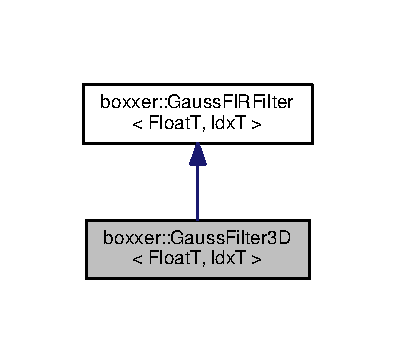
\includegraphics[width=190pt]{classboxxer_1_1GaussFilter3D__inherit__graph}
\end{center}
\end{figure}


Collaboration diagram for boxxer\+:\+:Gauss\+Filter3D$<$ FloatT, IdxT $>$\+:\nopagebreak
\begin{figure}[H]
\begin{center}
\leavevmode
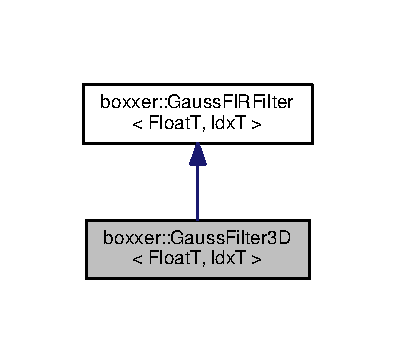
\includegraphics[width=190pt]{classboxxer_1_1GaussFilter3D__coll__graph}
\end{center}
\end{figure}
\subsubsection*{Public Types}
\begin{DoxyCompactItemize}
\item 
using \hyperlink{classboxxer_1_1GaussFilter3D_afcdf76336ad62fdc48a77672eea9a5b7}{I\+VecT} = typename \hyperlink{classboxxer_1_1GaussFIRFilter}{Gauss\+F\+I\+R\+Filter}$<$ FloatT, IdxT $>$\+::\hyperlink{classboxxer_1_1GaussFIRFilter_a0083c8c9ab6032dd458b4dc93852c2b8}{I\+VecT}
\item 
using \hyperlink{classboxxer_1_1GaussFilter3D_a0b98b323516d0fcb1422b10d63a70156}{VecT} = typename \hyperlink{classboxxer_1_1GaussFIRFilter}{Gauss\+F\+I\+R\+Filter}$<$ FloatT, IdxT $>$\+::\hyperlink{classboxxer_1_1GaussFilter3D_a0b98b323516d0fcb1422b10d63a70156}{VecT}
\item 
using \hyperlink{classboxxer_1_1GaussFilter3D_a62eb2a74863e76bd9237928521185d7a}{ImageT} = arma\+::\+Cube$<$ FloatT $>$
\item 
using \hyperlink{classboxxer_1_1GaussFIRFilter_a83cf4c7f4782f69918c0e0883fff5412}{MatT} = arma\+::\+Mat$<$ FloatT $>$
\end{DoxyCompactItemize}
\subsubsection*{Public Member Functions}
\begin{DoxyCompactItemize}
\item 
\hyperlink{classboxxer_1_1GaussFilter3D_acb9157d2158ac82264d2a3c849bd3ec3}{Gauss\+Filter3D} (const \hyperlink{classboxxer_1_1GaussFIRFilter_a0083c8c9ab6032dd458b4dc93852c2b8}{I\+VecT} \&\hyperlink{classboxxer_1_1GaussFIRFilter_ac0d4e19bb2be3e8913e77283e7e4317e}{size}, const \hyperlink{classboxxer_1_1GaussFilter3D_a0b98b323516d0fcb1422b10d63a70156}{VecT} \&\hyperlink{classboxxer_1_1GaussFIRFilter_a66ced06c688fd544d5f1f8be39aa2125}{sigma})
\item 
\hyperlink{classboxxer_1_1GaussFilter3D_a82355b9738082bade628c70c3077ff26}{Gauss\+Filter3D} (const \hyperlink{classboxxer_1_1GaussFIRFilter_a0083c8c9ab6032dd458b4dc93852c2b8}{I\+VecT} \&\hyperlink{classboxxer_1_1GaussFIRFilter_ac0d4e19bb2be3e8913e77283e7e4317e}{size}, const \hyperlink{classboxxer_1_1GaussFilter3D_a0b98b323516d0fcb1422b10d63a70156}{VecT} \&\hyperlink{classboxxer_1_1GaussFIRFilter_a66ced06c688fd544d5f1f8be39aa2125}{sigma}, const \hyperlink{classboxxer_1_1GaussFIRFilter_a0083c8c9ab6032dd458b4dc93852c2b8}{I\+VecT} \&kernel\+\_\+hw)
\item 
void \hyperlink{classboxxer_1_1GaussFilter3D_ac6d9013c566f27443b9e897ae58bcdd8}{set\+\_\+kernel\+\_\+hw} (const \hyperlink{classboxxer_1_1GaussFIRFilter_a0083c8c9ab6032dd458b4dc93852c2b8}{I\+VecT} \&kernel\+\_\+half\+\_\+width)
\item 
\hyperlink{classboxxer_1_1GaussFilter3D_a62eb2a74863e76bd9237928521185d7a}{ImageT} \hyperlink{classboxxer_1_1GaussFilter3D_af4298d5e1cf4f6f298d0f044d044e7c3}{make\+\_\+image} () const 
\item 
void \hyperlink{classboxxer_1_1GaussFilter3D_a3e909393e79507c03c6cfc25aeed5b8a}{filter} (const \hyperlink{classboxxer_1_1GaussFilter3D_a62eb2a74863e76bd9237928521185d7a}{ImageT} \&im, \hyperlink{classboxxer_1_1GaussFilter3D_a62eb2a74863e76bd9237928521185d7a}{ImageT} \&out)
\item 
void \hyperlink{classboxxer_1_1GaussFilter3D_a9b0e3c1d99cfa3a67c25f16c1a06182e}{test\+\_\+filter} (const \hyperlink{classboxxer_1_1GaussFilter3D_a62eb2a74863e76bd9237928521185d7a}{ImageT} \&im)
\end{DoxyCompactItemize}
\subsubsection*{Static Public Member Functions}
\begin{DoxyCompactItemize}
\item 
static \hyperlink{classboxxer_1_1GaussFilter3D_a0b98b323516d0fcb1422b10d63a70156}{VecT} \hyperlink{classboxxer_1_1GaussFIRFilter_a5dd6de5fe82092ec30141ab920d75dfd}{compute\+\_\+\+Gauss\+\_\+\+F\+I\+R\+\_\+kernel} (FloatT \hyperlink{classboxxer_1_1GaussFIRFilter_a66ced06c688fd544d5f1f8be39aa2125}{sigma}, IdxT \hyperlink{classboxxer_1_1GaussFIRFilter_ae17a4e137303e452a9223ba34825e0da}{hw})
\item 
static \hyperlink{classboxxer_1_1GaussFilter3D_a0b98b323516d0fcb1422b10d63a70156}{VecT} \hyperlink{classboxxer_1_1GaussFIRFilter_ad6a618b47db57b570278cc57b05d8c03}{compute\+\_\+\+Lo\+G\+\_\+\+F\+I\+R\+\_\+kernel} (FloatT \hyperlink{classboxxer_1_1GaussFIRFilter_a66ced06c688fd544d5f1f8be39aa2125}{sigma}, IdxT \hyperlink{classboxxer_1_1GaussFIRFilter_ae17a4e137303e452a9223ba34825e0da}{hw})
\end{DoxyCompactItemize}
\subsubsection*{Public Attributes}
\begin{DoxyCompactItemize}
\item 
IdxT \hyperlink{classboxxer_1_1GaussFIRFilter_ac7adcd4d8f8efee00a65262f596c8eda}{dim}
\item 
\hyperlink{classboxxer_1_1GaussFIRFilter_a0083c8c9ab6032dd458b4dc93852c2b8}{I\+VecT} \hyperlink{classboxxer_1_1GaussFIRFilter_ac0d4e19bb2be3e8913e77283e7e4317e}{size}
\item 
\hyperlink{classboxxer_1_1GaussFilter3D_a0b98b323516d0fcb1422b10d63a70156}{VecT} \hyperlink{classboxxer_1_1GaussFIRFilter_a66ced06c688fd544d5f1f8be39aa2125}{sigma}
\item 
\hyperlink{classboxxer_1_1GaussFIRFilter_a0083c8c9ab6032dd458b4dc93852c2b8}{I\+VecT} \hyperlink{classboxxer_1_1GaussFIRFilter_ae17a4e137303e452a9223ba34825e0da}{hw}
\end{DoxyCompactItemize}
\subsubsection*{Static Protected Attributes}
\begin{DoxyCompactItemize}
\item 
static const IdxT \hyperlink{classboxxer_1_1GaussFIRFilter_a7f85e018f78753ee4fedf65c04b0c65a}{max\+\_\+kernel\+\_\+hw}
\item 
static const FloatT \hyperlink{classboxxer_1_1GaussFIRFilter_a72b51cd7549510735179cb9c94f5f43f}{default\+\_\+sigma\+\_\+hw\+\_\+ratio}
\end{DoxyCompactItemize}
\subsubsection*{Friends}
\begin{DoxyCompactItemize}
\item 
{\footnotesize template$<$class Float\+T\+\_\+ , class Idx\+T\+\_\+ $>$ }\\std\+::ostream \& \hyperlink{classboxxer_1_1GaussFilter3D_a3e7ff88dad2f821551e56939779d24ba}{operator$<$$<$} (std\+::ostream \&out, const \hyperlink{classboxxer_1_1GaussFilter3D}{Gauss\+Filter3D}$<$ Float\+T\+\_\+, Idx\+T\+\_\+ $>$ \&filt)
\end{DoxyCompactItemize}


\subsubsection{Detailed Description}
\subsubsection*{template$<$class FloatT = float, class IdxT = uint32\+\_\+t$>$\\*
class boxxer\+::\+Gauss\+Filter3\+D$<$ Float\+T, Idx\+T $>$}

3D Filters 

Definition at line 126 of file Gauss\+Filter.\+h.



\subsubsection{Member Typedef Documentation}
\index{boxxer\+::\+Gauss\+Filter3D@{boxxer\+::\+Gauss\+Filter3D}!ImageT@{ImageT}}
\index{ImageT@{ImageT}!boxxer\+::\+Gauss\+Filter3D@{boxxer\+::\+Gauss\+Filter3D}}
\paragraph[{\texorpdfstring{ImageT}{ImageT}}]{\setlength{\rightskip}{0pt plus 5cm}template$<$class FloatT  = float, class IdxT  = uint32\+\_\+t$>$ using {\bf boxxer\+::\+Gauss\+Filter3D}$<$ FloatT, IdxT $>$\+::{\bf ImageT} =  arma\+::\+Cube$<$FloatT$>$}\hypertarget{classboxxer_1_1GaussFilter3D_a62eb2a74863e76bd9237928521185d7a}{}\label{classboxxer_1_1GaussFilter3D_a62eb2a74863e76bd9237928521185d7a}


Definition at line 131 of file Gauss\+Filter.\+h.

\index{boxxer\+::\+Gauss\+Filter3D@{boxxer\+::\+Gauss\+Filter3D}!I\+VecT@{I\+VecT}}
\index{I\+VecT@{I\+VecT}!boxxer\+::\+Gauss\+Filter3D@{boxxer\+::\+Gauss\+Filter3D}}
\paragraph[{\texorpdfstring{I\+VecT}{IVecT}}]{\setlength{\rightskip}{0pt plus 5cm}template$<$class FloatT  = float, class IdxT  = uint32\+\_\+t$>$ using {\bf boxxer\+::\+Gauss\+Filter3D}$<$ FloatT, IdxT $>$\+::{\bf I\+VecT} =  typename {\bf Gauss\+F\+I\+R\+Filter}$<$FloatT,IdxT$>$\+::{\bf I\+VecT}}\hypertarget{classboxxer_1_1GaussFilter3D_afcdf76336ad62fdc48a77672eea9a5b7}{}\label{classboxxer_1_1GaussFilter3D_afcdf76336ad62fdc48a77672eea9a5b7}


Definition at line 129 of file Gauss\+Filter.\+h.

\index{boxxer\+::\+Gauss\+Filter3D@{boxxer\+::\+Gauss\+Filter3D}!MatT@{MatT}}
\index{MatT@{MatT}!boxxer\+::\+Gauss\+Filter3D@{boxxer\+::\+Gauss\+Filter3D}}
\paragraph[{\texorpdfstring{MatT}{MatT}}]{\setlength{\rightskip}{0pt plus 5cm}template$<$class FloatT = float, class IdxT = uint32\+\_\+t$>$ using {\bf boxxer\+::\+Gauss\+F\+I\+R\+Filter}$<$ FloatT, IdxT $>$\+::{\bf MatT} =  arma\+::\+Mat$<$FloatT$>$\hspace{0.3cm}{\ttfamily [inherited]}}\hypertarget{classboxxer_1_1GaussFIRFilter_a83cf4c7f4782f69918c0e0883fff5412}{}\label{classboxxer_1_1GaussFIRFilter_a83cf4c7f4782f69918c0e0883fff5412}


Definition at line 26 of file Gauss\+Filter.\+h.

\index{boxxer\+::\+Gauss\+Filter3D@{boxxer\+::\+Gauss\+Filter3D}!VecT@{VecT}}
\index{VecT@{VecT}!boxxer\+::\+Gauss\+Filter3D@{boxxer\+::\+Gauss\+Filter3D}}
\paragraph[{\texorpdfstring{VecT}{VecT}}]{\setlength{\rightskip}{0pt plus 5cm}template$<$class FloatT  = float, class IdxT  = uint32\+\_\+t$>$ using {\bf boxxer\+::\+Gauss\+Filter3D}$<$ FloatT, IdxT $>$\+::{\bf VecT} =  typename {\bf Gauss\+F\+I\+R\+Filter}$<$FloatT,IdxT$>$\+::{\bf VecT}}\hypertarget{classboxxer_1_1GaussFilter3D_a0b98b323516d0fcb1422b10d63a70156}{}\label{classboxxer_1_1GaussFilter3D_a0b98b323516d0fcb1422b10d63a70156}


Definition at line 130 of file Gauss\+Filter.\+h.



\subsubsection{Constructor \& Destructor Documentation}
\index{boxxer\+::\+Gauss\+Filter3D@{boxxer\+::\+Gauss\+Filter3D}!Gauss\+Filter3D@{Gauss\+Filter3D}}
\index{Gauss\+Filter3D@{Gauss\+Filter3D}!boxxer\+::\+Gauss\+Filter3D@{boxxer\+::\+Gauss\+Filter3D}}
\paragraph[{\texorpdfstring{Gauss\+Filter3\+D(const I\+Vec\+T \&size, const Vec\+T \&sigma)}{GaussFilter3D(const IVecT &size, const VecT &sigma)}}]{\setlength{\rightskip}{0pt plus 5cm}template$<$class FloatT  = float, class IdxT  = uint32\+\_\+t$>$ {\bf boxxer\+::\+Gauss\+Filter3D}$<$ FloatT, IdxT $>$\+::{\bf Gauss\+Filter3D} (
\begin{DoxyParamCaption}
\item[{const {\bf I\+VecT} \&}]{size, }
\item[{const {\bf VecT} \&}]{sigma}
\end{DoxyParamCaption}
)}\hypertarget{classboxxer_1_1GaussFilter3D_acb9157d2158ac82264d2a3c849bd3ec3}{}\label{classboxxer_1_1GaussFilter3D_acb9157d2158ac82264d2a3c849bd3ec3}
\index{boxxer\+::\+Gauss\+Filter3D@{boxxer\+::\+Gauss\+Filter3D}!Gauss\+Filter3D@{Gauss\+Filter3D}}
\index{Gauss\+Filter3D@{Gauss\+Filter3D}!boxxer\+::\+Gauss\+Filter3D@{boxxer\+::\+Gauss\+Filter3D}}
\paragraph[{\texorpdfstring{Gauss\+Filter3\+D(const I\+Vec\+T \&size, const Vec\+T \&sigma, const I\+Vec\+T \&kernel\+\_\+hw)}{GaussFilter3D(const IVecT &size, const VecT &sigma, const IVecT &kernel_hw)}}]{\setlength{\rightskip}{0pt plus 5cm}template$<$class FloatT  = float, class IdxT  = uint32\+\_\+t$>$ {\bf boxxer\+::\+Gauss\+Filter3D}$<$ FloatT, IdxT $>$\+::{\bf Gauss\+Filter3D} (
\begin{DoxyParamCaption}
\item[{const {\bf I\+VecT} \&}]{size, }
\item[{const {\bf VecT} \&}]{sigma, }
\item[{const {\bf I\+VecT} \&}]{kernel\+\_\+hw}
\end{DoxyParamCaption}
)}\hypertarget{classboxxer_1_1GaussFilter3D_a82355b9738082bade628c70c3077ff26}{}\label{classboxxer_1_1GaussFilter3D_a82355b9738082bade628c70c3077ff26}


\subsubsection{Member Function Documentation}
\index{boxxer\+::\+Gauss\+Filter3D@{boxxer\+::\+Gauss\+Filter3D}!compute\+\_\+\+Gauss\+\_\+\+F\+I\+R\+\_\+kernel@{compute\+\_\+\+Gauss\+\_\+\+F\+I\+R\+\_\+kernel}}
\index{compute\+\_\+\+Gauss\+\_\+\+F\+I\+R\+\_\+kernel@{compute\+\_\+\+Gauss\+\_\+\+F\+I\+R\+\_\+kernel}!boxxer\+::\+Gauss\+Filter3D@{boxxer\+::\+Gauss\+Filter3D}}
\paragraph[{\texorpdfstring{compute\+\_\+\+Gauss\+\_\+\+F\+I\+R\+\_\+kernel(\+Float\+T sigma, Idx\+T hw)}{compute_Gauss_FIR_kernel(FloatT sigma, IdxT hw)}}]{\setlength{\rightskip}{0pt plus 5cm}template$<$class FloatT = float, class IdxT = uint32\+\_\+t$>$ static {\bf VecT} {\bf boxxer\+::\+Gauss\+F\+I\+R\+Filter}$<$ FloatT, IdxT $>$\+::compute\+\_\+\+Gauss\+\_\+\+F\+I\+R\+\_\+kernel (
\begin{DoxyParamCaption}
\item[{FloatT}]{sigma, }
\item[{IdxT}]{hw}
\end{DoxyParamCaption}
)\hspace{0.3cm}{\ttfamily [static]}, {\ttfamily [inherited]}}\hypertarget{classboxxer_1_1GaussFIRFilter_a5dd6de5fe82092ec30141ab920d75dfd}{}\label{classboxxer_1_1GaussFIRFilter_a5dd6de5fe82092ec30141ab920d75dfd}
\index{boxxer\+::\+Gauss\+Filter3D@{boxxer\+::\+Gauss\+Filter3D}!compute\+\_\+\+Lo\+G\+\_\+\+F\+I\+R\+\_\+kernel@{compute\+\_\+\+Lo\+G\+\_\+\+F\+I\+R\+\_\+kernel}}
\index{compute\+\_\+\+Lo\+G\+\_\+\+F\+I\+R\+\_\+kernel@{compute\+\_\+\+Lo\+G\+\_\+\+F\+I\+R\+\_\+kernel}!boxxer\+::\+Gauss\+Filter3D@{boxxer\+::\+Gauss\+Filter3D}}
\paragraph[{\texorpdfstring{compute\+\_\+\+Lo\+G\+\_\+\+F\+I\+R\+\_\+kernel(\+Float\+T sigma, Idx\+T hw)}{compute_LoG_FIR_kernel(FloatT sigma, IdxT hw)}}]{\setlength{\rightskip}{0pt plus 5cm}template$<$class FloatT = float, class IdxT = uint32\+\_\+t$>$ static {\bf VecT} {\bf boxxer\+::\+Gauss\+F\+I\+R\+Filter}$<$ FloatT, IdxT $>$\+::compute\+\_\+\+Lo\+G\+\_\+\+F\+I\+R\+\_\+kernel (
\begin{DoxyParamCaption}
\item[{FloatT}]{sigma, }
\item[{IdxT}]{hw}
\end{DoxyParamCaption}
)\hspace{0.3cm}{\ttfamily [static]}, {\ttfamily [inherited]}}\hypertarget{classboxxer_1_1GaussFIRFilter_ad6a618b47db57b570278cc57b05d8c03}{}\label{classboxxer_1_1GaussFIRFilter_ad6a618b47db57b570278cc57b05d8c03}
\index{boxxer\+::\+Gauss\+Filter3D@{boxxer\+::\+Gauss\+Filter3D}!filter@{filter}}
\index{filter@{filter}!boxxer\+::\+Gauss\+Filter3D@{boxxer\+::\+Gauss\+Filter3D}}
\paragraph[{\texorpdfstring{filter(const Image\+T \&im, Image\+T \&out)}{filter(const ImageT &im, ImageT &out)}}]{\setlength{\rightskip}{0pt plus 5cm}template$<$class FloatT  = float, class IdxT  = uint32\+\_\+t$>$ void {\bf boxxer\+::\+Gauss\+Filter3D}$<$ FloatT, IdxT $>$\+::filter (
\begin{DoxyParamCaption}
\item[{const {\bf ImageT} \&}]{im, }
\item[{{\bf ImageT} \&}]{out}
\end{DoxyParamCaption}
)}\hypertarget{classboxxer_1_1GaussFilter3D_a3e909393e79507c03c6cfc25aeed5b8a}{}\label{classboxxer_1_1GaussFilter3D_a3e909393e79507c03c6cfc25aeed5b8a}
\index{boxxer\+::\+Gauss\+Filter3D@{boxxer\+::\+Gauss\+Filter3D}!make\+\_\+image@{make\+\_\+image}}
\index{make\+\_\+image@{make\+\_\+image}!boxxer\+::\+Gauss\+Filter3D@{boxxer\+::\+Gauss\+Filter3D}}
\paragraph[{\texorpdfstring{make\+\_\+image() const }{make_image() const }}]{\setlength{\rightskip}{0pt plus 5cm}template$<$class FloatT  = float, class IdxT  = uint32\+\_\+t$>$ {\bf ImageT} {\bf boxxer\+::\+Gauss\+Filter3D}$<$ FloatT, IdxT $>$\+::make\+\_\+image (
\begin{DoxyParamCaption}
{}
\end{DoxyParamCaption}
) const\hspace{0.3cm}{\ttfamily [inline]}}\hypertarget{classboxxer_1_1GaussFilter3D_af4298d5e1cf4f6f298d0f044d044e7c3}{}\label{classboxxer_1_1GaussFilter3D_af4298d5e1cf4f6f298d0f044d044e7c3}


Definition at line 136 of file Gauss\+Filter.\+h.



References boxxer\+::\+Gauss\+F\+I\+R\+Filter$<$ Float\+T, Idx\+T $>$\+::size.

\index{boxxer\+::\+Gauss\+Filter3D@{boxxer\+::\+Gauss\+Filter3D}!set\+\_\+kernel\+\_\+hw@{set\+\_\+kernel\+\_\+hw}}
\index{set\+\_\+kernel\+\_\+hw@{set\+\_\+kernel\+\_\+hw}!boxxer\+::\+Gauss\+Filter3D@{boxxer\+::\+Gauss\+Filter3D}}
\paragraph[{\texorpdfstring{set\+\_\+kernel\+\_\+hw(const I\+Vec\+T \&kernel\+\_\+half\+\_\+width)}{set_kernel_hw(const IVecT &kernel_half_width)}}]{\setlength{\rightskip}{0pt plus 5cm}template$<$class FloatT  = float, class IdxT  = uint32\+\_\+t$>$ void {\bf boxxer\+::\+Gauss\+Filter3D}$<$ FloatT, IdxT $>$\+::set\+\_\+kernel\+\_\+hw (
\begin{DoxyParamCaption}
\item[{const {\bf I\+VecT} \&}]{kernel\+\_\+half\+\_\+width}
\end{DoxyParamCaption}
)\hspace{0.3cm}{\ttfamily [virtual]}}\hypertarget{classboxxer_1_1GaussFilter3D_ac6d9013c566f27443b9e897ae58bcdd8}{}\label{classboxxer_1_1GaussFilter3D_ac6d9013c566f27443b9e897ae58bcdd8}


Implements \hyperlink{classboxxer_1_1GaussFIRFilter_a7ada113680b67f052d11afe346ddf8bc}{boxxer\+::\+Gauss\+F\+I\+R\+Filter$<$ Float\+T, Idx\+T $>$}.

\index{boxxer\+::\+Gauss\+Filter3D@{boxxer\+::\+Gauss\+Filter3D}!test\+\_\+filter@{test\+\_\+filter}}
\index{test\+\_\+filter@{test\+\_\+filter}!boxxer\+::\+Gauss\+Filter3D@{boxxer\+::\+Gauss\+Filter3D}}
\paragraph[{\texorpdfstring{test\+\_\+filter(const Image\+T \&im)}{test_filter(const ImageT &im)}}]{\setlength{\rightskip}{0pt plus 5cm}template$<$class FloatT  = float, class IdxT  = uint32\+\_\+t$>$ void {\bf boxxer\+::\+Gauss\+Filter3D}$<$ FloatT, IdxT $>$\+::test\+\_\+filter (
\begin{DoxyParamCaption}
\item[{const {\bf ImageT} \&}]{im}
\end{DoxyParamCaption}
)}\hypertarget{classboxxer_1_1GaussFilter3D_a9b0e3c1d99cfa3a67c25f16c1a06182e}{}\label{classboxxer_1_1GaussFilter3D_a9b0e3c1d99cfa3a67c25f16c1a06182e}


\subsubsection{Friends And Related Function Documentation}
\index{boxxer\+::\+Gauss\+Filter3D@{boxxer\+::\+Gauss\+Filter3D}!operator$<$$<$@{operator$<$$<$}}
\index{operator$<$$<$@{operator$<$$<$}!boxxer\+::\+Gauss\+Filter3D@{boxxer\+::\+Gauss\+Filter3D}}
\paragraph[{\texorpdfstring{operator$<$$<$}{operator<<}}]{\setlength{\rightskip}{0pt plus 5cm}template$<$class FloatT  = float, class IdxT  = uint32\+\_\+t$>$ template$<$class Float\+T\+\_\+ , class Idx\+T\+\_\+ $>$ std\+::ostream\& operator$<$$<$ (
\begin{DoxyParamCaption}
\item[{std\+::ostream \&}]{out, }
\item[{const {\bf Gauss\+Filter3D}$<$ Float\+T\+\_\+, Idx\+T\+\_\+ $>$ \&}]{filt}
\end{DoxyParamCaption}
)\hspace{0.3cm}{\ttfamily [friend]}}\hypertarget{classboxxer_1_1GaussFilter3D_a3e7ff88dad2f821551e56939779d24ba}{}\label{classboxxer_1_1GaussFilter3D_a3e7ff88dad2f821551e56939779d24ba}


\subsubsection{Member Data Documentation}
\index{boxxer\+::\+Gauss\+Filter3D@{boxxer\+::\+Gauss\+Filter3D}!default\+\_\+sigma\+\_\+hw\+\_\+ratio@{default\+\_\+sigma\+\_\+hw\+\_\+ratio}}
\index{default\+\_\+sigma\+\_\+hw\+\_\+ratio@{default\+\_\+sigma\+\_\+hw\+\_\+ratio}!boxxer\+::\+Gauss\+Filter3D@{boxxer\+::\+Gauss\+Filter3D}}
\paragraph[{\texorpdfstring{default\+\_\+sigma\+\_\+hw\+\_\+ratio}{default_sigma_hw_ratio}}]{\setlength{\rightskip}{0pt plus 5cm}template$<$class FloatT = float, class IdxT = uint32\+\_\+t$>$ const FloatT {\bf boxxer\+::\+Gauss\+F\+I\+R\+Filter}$<$ FloatT, IdxT $>$\+::default\+\_\+sigma\+\_\+hw\+\_\+ratio\hspace{0.3cm}{\ttfamily [static]}, {\ttfamily [protected]}, {\ttfamily [inherited]}}\hypertarget{classboxxer_1_1GaussFIRFilter_a72b51cd7549510735179cb9c94f5f43f}{}\label{classboxxer_1_1GaussFIRFilter_a72b51cd7549510735179cb9c94f5f43f}


Definition at line 41 of file Gauss\+Filter.\+h.

\index{boxxer\+::\+Gauss\+Filter3D@{boxxer\+::\+Gauss\+Filter3D}!dim@{dim}}
\index{dim@{dim}!boxxer\+::\+Gauss\+Filter3D@{boxxer\+::\+Gauss\+Filter3D}}
\paragraph[{\texorpdfstring{dim}{dim}}]{\setlength{\rightskip}{0pt plus 5cm}template$<$class FloatT = float, class IdxT = uint32\+\_\+t$>$ IdxT {\bf boxxer\+::\+Gauss\+F\+I\+R\+Filter}$<$ FloatT, IdxT $>$\+::dim\hspace{0.3cm}{\ttfamily [inherited]}}\hypertarget{classboxxer_1_1GaussFIRFilter_ac7adcd4d8f8efee00a65262f596c8eda}{}\label{classboxxer_1_1GaussFIRFilter_ac7adcd4d8f8efee00a65262f596c8eda}


Definition at line 28 of file Gauss\+Filter.\+h.

\index{boxxer\+::\+Gauss\+Filter3D@{boxxer\+::\+Gauss\+Filter3D}!hw@{hw}}
\index{hw@{hw}!boxxer\+::\+Gauss\+Filter3D@{boxxer\+::\+Gauss\+Filter3D}}
\paragraph[{\texorpdfstring{hw}{hw}}]{\setlength{\rightskip}{0pt plus 5cm}template$<$class FloatT = float, class IdxT = uint32\+\_\+t$>$ {\bf I\+VecT} {\bf boxxer\+::\+Gauss\+F\+I\+R\+Filter}$<$ FloatT, IdxT $>$\+::hw\hspace{0.3cm}{\ttfamily [inherited]}}\hypertarget{classboxxer_1_1GaussFIRFilter_ae17a4e137303e452a9223ba34825e0da}{}\label{classboxxer_1_1GaussFIRFilter_ae17a4e137303e452a9223ba34825e0da}


Definition at line 31 of file Gauss\+Filter.\+h.

\index{boxxer\+::\+Gauss\+Filter3D@{boxxer\+::\+Gauss\+Filter3D}!max\+\_\+kernel\+\_\+hw@{max\+\_\+kernel\+\_\+hw}}
\index{max\+\_\+kernel\+\_\+hw@{max\+\_\+kernel\+\_\+hw}!boxxer\+::\+Gauss\+Filter3D@{boxxer\+::\+Gauss\+Filter3D}}
\paragraph[{\texorpdfstring{max\+\_\+kernel\+\_\+hw}{max_kernel_hw}}]{\setlength{\rightskip}{0pt plus 5cm}template$<$class FloatT = float, class IdxT = uint32\+\_\+t$>$ const IdxT {\bf boxxer\+::\+Gauss\+F\+I\+R\+Filter}$<$ FloatT, IdxT $>$\+::max\+\_\+kernel\+\_\+hw\hspace{0.3cm}{\ttfamily [static]}, {\ttfamily [protected]}, {\ttfamily [inherited]}}\hypertarget{classboxxer_1_1GaussFIRFilter_a7f85e018f78753ee4fedf65c04b0c65a}{}\label{classboxxer_1_1GaussFIRFilter_a7f85e018f78753ee4fedf65c04b0c65a}


Definition at line 40 of file Gauss\+Filter.\+h.

\index{boxxer\+::\+Gauss\+Filter3D@{boxxer\+::\+Gauss\+Filter3D}!sigma@{sigma}}
\index{sigma@{sigma}!boxxer\+::\+Gauss\+Filter3D@{boxxer\+::\+Gauss\+Filter3D}}
\paragraph[{\texorpdfstring{sigma}{sigma}}]{\setlength{\rightskip}{0pt plus 5cm}template$<$class FloatT = float, class IdxT = uint32\+\_\+t$>$ {\bf VecT} {\bf boxxer\+::\+Gauss\+F\+I\+R\+Filter}$<$ FloatT, IdxT $>$\+::sigma\hspace{0.3cm}{\ttfamily [inherited]}}\hypertarget{classboxxer_1_1GaussFIRFilter_a66ced06c688fd544d5f1f8be39aa2125}{}\label{classboxxer_1_1GaussFIRFilter_a66ced06c688fd544d5f1f8be39aa2125}


Definition at line 30 of file Gauss\+Filter.\+h.

\index{boxxer\+::\+Gauss\+Filter3D@{boxxer\+::\+Gauss\+Filter3D}!size@{size}}
\index{size@{size}!boxxer\+::\+Gauss\+Filter3D@{boxxer\+::\+Gauss\+Filter3D}}
\paragraph[{\texorpdfstring{size}{size}}]{\setlength{\rightskip}{0pt plus 5cm}template$<$class FloatT = float, class IdxT = uint32\+\_\+t$>$ {\bf I\+VecT} {\bf boxxer\+::\+Gauss\+F\+I\+R\+Filter}$<$ FloatT, IdxT $>$\+::size\hspace{0.3cm}{\ttfamily [inherited]}}\hypertarget{classboxxer_1_1GaussFIRFilter_ac0d4e19bb2be3e8913e77283e7e4317e}{}\label{classboxxer_1_1GaussFIRFilter_ac0d4e19bb2be3e8913e77283e7e4317e}


Definition at line 29 of file Gauss\+Filter.\+h.



Referenced by boxxer\+::\+Gauss\+Filter2\+D$<$ Float\+T, Idx\+T $>$\+::make\+\_\+image(), boxxer\+::\+Do\+G\+Filter2\+D$<$ Float\+T, Idx\+T $>$\+::make\+\_\+image(), boxxer\+::\+Lo\+G\+Filter2\+D$<$ Float\+T, Idx\+T $>$\+::make\+\_\+image(), boxxer\+::\+Gauss\+Filter3\+D$<$ Float\+T, Idx\+T $>$\+::make\+\_\+image(), boxxer\+::\+Do\+G\+Filter3\+D$<$ Float\+T, Idx\+T $>$\+::make\+\_\+image(), and boxxer\+::\+Lo\+G\+Filter3\+D$<$ Float\+T, Idx\+T $>$\+::make\+\_\+image().



The documentation for this class was generated from the following file\+:\begin{DoxyCompactItemize}
\item 
\hyperlink{GaussFilter_8h}{Gauss\+Filter.\+h}\end{DoxyCompactItemize}

\hypertarget{classboxxer_1_1GaussFIRFilter}{}\subsection{boxxer\+:\+:Gauss\+F\+I\+R\+Filter$<$ FloatT, IdxT $>$ Class Template Reference}
\label{classboxxer_1_1GaussFIRFilter}\index{boxxer\+::\+Gauss\+F\+I\+R\+Filter$<$ Float\+T, Idx\+T $>$@{boxxer\+::\+Gauss\+F\+I\+R\+Filter$<$ Float\+T, Idx\+T $>$}}


{\ttfamily \#include $<$/home/travis/build/markjolah/\+Boxxer/include/\+Boxxer/\+Gauss\+Filter.\+h$>$}



Inheritance diagram for boxxer\+:\+:Gauss\+F\+I\+R\+Filter$<$ FloatT, IdxT $>$\+:\nopagebreak
\begin{figure}[H]
\begin{center}
\leavevmode
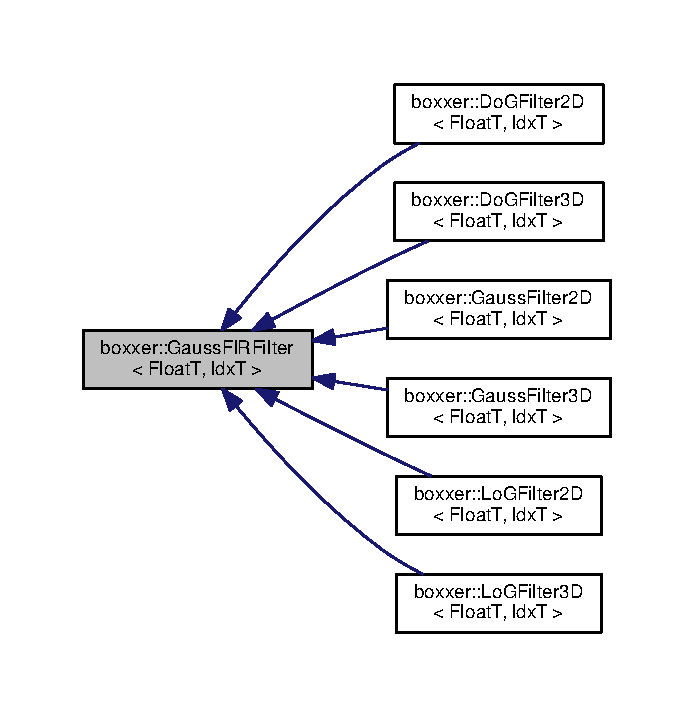
\includegraphics[width=333pt]{classboxxer_1_1GaussFIRFilter__inherit__graph}
\end{center}
\end{figure}
\subsubsection*{Public Types}
\begin{DoxyCompactItemize}
\item 
using \hyperlink{classboxxer_1_1GaussFIRFilter_a0083c8c9ab6032dd458b4dc93852c2b8}{I\+VecT} = arma\+::\+Col$<$ IdxT $>$
\item 
using \hyperlink{classboxxer_1_1GaussFIRFilter_aafe2049df690ad8c3617c39810e78bbe}{VecT} = arma\+::\+Col$<$ FloatT $>$
\item 
using \hyperlink{classboxxer_1_1GaussFIRFilter_a83cf4c7f4782f69918c0e0883fff5412}{MatT} = arma\+::\+Mat$<$ FloatT $>$
\end{DoxyCompactItemize}
\subsubsection*{Public Member Functions}
\begin{DoxyCompactItemize}
\item 
\hyperlink{classboxxer_1_1GaussFIRFilter_a4c1a2a3cd8578b90ccea9efc6f3a3c97}{Gauss\+F\+I\+R\+Filter} (IdxT \hyperlink{classboxxer_1_1GaussFIRFilter_ac7adcd4d8f8efee00a65262f596c8eda}{dim}, const \hyperlink{classboxxer_1_1GaussFIRFilter_a0083c8c9ab6032dd458b4dc93852c2b8}{I\+VecT} \&\hyperlink{classboxxer_1_1GaussFIRFilter_ac0d4e19bb2be3e8913e77283e7e4317e}{size}, const \hyperlink{classboxxer_1_1GaussFIRFilter_aafe2049df690ad8c3617c39810e78bbe}{VecT} \&\hyperlink{classboxxer_1_1GaussFIRFilter_a66ced06c688fd544d5f1f8be39aa2125}{sigma})
\item 
virtual void \hyperlink{classboxxer_1_1GaussFIRFilter_a7ada113680b67f052d11afe346ddf8bc}{set\+\_\+kernel\+\_\+hw} (const \hyperlink{classboxxer_1_1GaussFIRFilter_a0083c8c9ab6032dd458b4dc93852c2b8}{I\+VecT} \&kernel\+\_\+half\+\_\+width)=0
\end{DoxyCompactItemize}
\subsubsection*{Static Public Member Functions}
\begin{DoxyCompactItemize}
\item 
static \hyperlink{classboxxer_1_1GaussFIRFilter_aafe2049df690ad8c3617c39810e78bbe}{VecT} \hyperlink{classboxxer_1_1GaussFIRFilter_a5dd6de5fe82092ec30141ab920d75dfd}{compute\+\_\+\+Gauss\+\_\+\+F\+I\+R\+\_\+kernel} (FloatT \hyperlink{classboxxer_1_1GaussFIRFilter_a66ced06c688fd544d5f1f8be39aa2125}{sigma}, IdxT \hyperlink{classboxxer_1_1GaussFIRFilter_ae17a4e137303e452a9223ba34825e0da}{hw})
\item 
static \hyperlink{classboxxer_1_1GaussFIRFilter_aafe2049df690ad8c3617c39810e78bbe}{VecT} \hyperlink{classboxxer_1_1GaussFIRFilter_ad6a618b47db57b570278cc57b05d8c03}{compute\+\_\+\+Lo\+G\+\_\+\+F\+I\+R\+\_\+kernel} (FloatT \hyperlink{classboxxer_1_1GaussFIRFilter_a66ced06c688fd544d5f1f8be39aa2125}{sigma}, IdxT \hyperlink{classboxxer_1_1GaussFIRFilter_ae17a4e137303e452a9223ba34825e0da}{hw})
\end{DoxyCompactItemize}
\subsubsection*{Public Attributes}
\begin{DoxyCompactItemize}
\item 
IdxT \hyperlink{classboxxer_1_1GaussFIRFilter_ac7adcd4d8f8efee00a65262f596c8eda}{dim}
\item 
\hyperlink{classboxxer_1_1GaussFIRFilter_a0083c8c9ab6032dd458b4dc93852c2b8}{I\+VecT} \hyperlink{classboxxer_1_1GaussFIRFilter_ac0d4e19bb2be3e8913e77283e7e4317e}{size}
\item 
\hyperlink{classboxxer_1_1GaussFIRFilter_aafe2049df690ad8c3617c39810e78bbe}{VecT} \hyperlink{classboxxer_1_1GaussFIRFilter_a66ced06c688fd544d5f1f8be39aa2125}{sigma}
\item 
\hyperlink{classboxxer_1_1GaussFIRFilter_a0083c8c9ab6032dd458b4dc93852c2b8}{I\+VecT} \hyperlink{classboxxer_1_1GaussFIRFilter_ae17a4e137303e452a9223ba34825e0da}{hw}
\end{DoxyCompactItemize}
\subsubsection*{Static Protected Attributes}
\begin{DoxyCompactItemize}
\item 
static const IdxT \hyperlink{classboxxer_1_1GaussFIRFilter_a7f85e018f78753ee4fedf65c04b0c65a}{max\+\_\+kernel\+\_\+hw}
\item 
static const FloatT \hyperlink{classboxxer_1_1GaussFIRFilter_a72b51cd7549510735179cb9c94f5f43f}{default\+\_\+sigma\+\_\+hw\+\_\+ratio}
\end{DoxyCompactItemize}


\subsubsection{Detailed Description}
\subsubsection*{template$<$class FloatT = float, class IdxT = uint32\+\_\+t$>$\\*
class boxxer\+::\+Gauss\+F\+I\+R\+Filter$<$ Float\+T, Idx\+T $>$}

Base filters 

Definition at line 21 of file Gauss\+Filter.\+h.



\subsubsection{Member Typedef Documentation}
\index{boxxer\+::\+Gauss\+F\+I\+R\+Filter@{boxxer\+::\+Gauss\+F\+I\+R\+Filter}!I\+VecT@{I\+VecT}}
\index{I\+VecT@{I\+VecT}!boxxer\+::\+Gauss\+F\+I\+R\+Filter@{boxxer\+::\+Gauss\+F\+I\+R\+Filter}}
\paragraph[{\texorpdfstring{I\+VecT}{IVecT}}]{\setlength{\rightskip}{0pt plus 5cm}template$<$class FloatT = float, class IdxT = uint32\+\_\+t$>$ using {\bf boxxer\+::\+Gauss\+F\+I\+R\+Filter}$<$ FloatT, IdxT $>$\+::{\bf I\+VecT} =  arma\+::\+Col$<$IdxT$>$}\hypertarget{classboxxer_1_1GaussFIRFilter_a0083c8c9ab6032dd458b4dc93852c2b8}{}\label{classboxxer_1_1GaussFIRFilter_a0083c8c9ab6032dd458b4dc93852c2b8}


Definition at line 24 of file Gauss\+Filter.\+h.

\index{boxxer\+::\+Gauss\+F\+I\+R\+Filter@{boxxer\+::\+Gauss\+F\+I\+R\+Filter}!MatT@{MatT}}
\index{MatT@{MatT}!boxxer\+::\+Gauss\+F\+I\+R\+Filter@{boxxer\+::\+Gauss\+F\+I\+R\+Filter}}
\paragraph[{\texorpdfstring{MatT}{MatT}}]{\setlength{\rightskip}{0pt plus 5cm}template$<$class FloatT = float, class IdxT = uint32\+\_\+t$>$ using {\bf boxxer\+::\+Gauss\+F\+I\+R\+Filter}$<$ FloatT, IdxT $>$\+::{\bf MatT} =  arma\+::\+Mat$<$FloatT$>$}\hypertarget{classboxxer_1_1GaussFIRFilter_a83cf4c7f4782f69918c0e0883fff5412}{}\label{classboxxer_1_1GaussFIRFilter_a83cf4c7f4782f69918c0e0883fff5412}


Definition at line 26 of file Gauss\+Filter.\+h.

\index{boxxer\+::\+Gauss\+F\+I\+R\+Filter@{boxxer\+::\+Gauss\+F\+I\+R\+Filter}!VecT@{VecT}}
\index{VecT@{VecT}!boxxer\+::\+Gauss\+F\+I\+R\+Filter@{boxxer\+::\+Gauss\+F\+I\+R\+Filter}}
\paragraph[{\texorpdfstring{VecT}{VecT}}]{\setlength{\rightskip}{0pt plus 5cm}template$<$class FloatT = float, class IdxT = uint32\+\_\+t$>$ using {\bf boxxer\+::\+Gauss\+F\+I\+R\+Filter}$<$ FloatT, IdxT $>$\+::{\bf VecT} =  arma\+::\+Col$<$FloatT$>$}\hypertarget{classboxxer_1_1GaussFIRFilter_aafe2049df690ad8c3617c39810e78bbe}{}\label{classboxxer_1_1GaussFIRFilter_aafe2049df690ad8c3617c39810e78bbe}


Definition at line 25 of file Gauss\+Filter.\+h.



\subsubsection{Constructor \& Destructor Documentation}
\index{boxxer\+::\+Gauss\+F\+I\+R\+Filter@{boxxer\+::\+Gauss\+F\+I\+R\+Filter}!Gauss\+F\+I\+R\+Filter@{Gauss\+F\+I\+R\+Filter}}
\index{Gauss\+F\+I\+R\+Filter@{Gauss\+F\+I\+R\+Filter}!boxxer\+::\+Gauss\+F\+I\+R\+Filter@{boxxer\+::\+Gauss\+F\+I\+R\+Filter}}
\paragraph[{\texorpdfstring{Gauss\+F\+I\+R\+Filter(\+Idx\+T dim, const I\+Vec\+T \&size, const Vec\+T \&sigma)}{GaussFIRFilter(IdxT dim, const IVecT &size, const VecT &sigma)}}]{\setlength{\rightskip}{0pt plus 5cm}template$<$class FloatT = float, class IdxT = uint32\+\_\+t$>$ {\bf boxxer\+::\+Gauss\+F\+I\+R\+Filter}$<$ FloatT, IdxT $>$\+::{\bf Gauss\+F\+I\+R\+Filter} (
\begin{DoxyParamCaption}
\item[{IdxT}]{dim, }
\item[{const {\bf I\+VecT} \&}]{size, }
\item[{const {\bf VecT} \&}]{sigma}
\end{DoxyParamCaption}
)}\hypertarget{classboxxer_1_1GaussFIRFilter_a4c1a2a3cd8578b90ccea9efc6f3a3c97}{}\label{classboxxer_1_1GaussFIRFilter_a4c1a2a3cd8578b90ccea9efc6f3a3c97}


\subsubsection{Member Function Documentation}
\index{boxxer\+::\+Gauss\+F\+I\+R\+Filter@{boxxer\+::\+Gauss\+F\+I\+R\+Filter}!compute\+\_\+\+Gauss\+\_\+\+F\+I\+R\+\_\+kernel@{compute\+\_\+\+Gauss\+\_\+\+F\+I\+R\+\_\+kernel}}
\index{compute\+\_\+\+Gauss\+\_\+\+F\+I\+R\+\_\+kernel@{compute\+\_\+\+Gauss\+\_\+\+F\+I\+R\+\_\+kernel}!boxxer\+::\+Gauss\+F\+I\+R\+Filter@{boxxer\+::\+Gauss\+F\+I\+R\+Filter}}
\paragraph[{\texorpdfstring{compute\+\_\+\+Gauss\+\_\+\+F\+I\+R\+\_\+kernel(\+Float\+T sigma, Idx\+T hw)}{compute_Gauss_FIR_kernel(FloatT sigma, IdxT hw)}}]{\setlength{\rightskip}{0pt plus 5cm}template$<$class FloatT = float, class IdxT = uint32\+\_\+t$>$ static {\bf VecT} {\bf boxxer\+::\+Gauss\+F\+I\+R\+Filter}$<$ FloatT, IdxT $>$\+::compute\+\_\+\+Gauss\+\_\+\+F\+I\+R\+\_\+kernel (
\begin{DoxyParamCaption}
\item[{FloatT}]{sigma, }
\item[{IdxT}]{hw}
\end{DoxyParamCaption}
)\hspace{0.3cm}{\ttfamily [static]}}\hypertarget{classboxxer_1_1GaussFIRFilter_a5dd6de5fe82092ec30141ab920d75dfd}{}\label{classboxxer_1_1GaussFIRFilter_a5dd6de5fe82092ec30141ab920d75dfd}
\index{boxxer\+::\+Gauss\+F\+I\+R\+Filter@{boxxer\+::\+Gauss\+F\+I\+R\+Filter}!compute\+\_\+\+Lo\+G\+\_\+\+F\+I\+R\+\_\+kernel@{compute\+\_\+\+Lo\+G\+\_\+\+F\+I\+R\+\_\+kernel}}
\index{compute\+\_\+\+Lo\+G\+\_\+\+F\+I\+R\+\_\+kernel@{compute\+\_\+\+Lo\+G\+\_\+\+F\+I\+R\+\_\+kernel}!boxxer\+::\+Gauss\+F\+I\+R\+Filter@{boxxer\+::\+Gauss\+F\+I\+R\+Filter}}
\paragraph[{\texorpdfstring{compute\+\_\+\+Lo\+G\+\_\+\+F\+I\+R\+\_\+kernel(\+Float\+T sigma, Idx\+T hw)}{compute_LoG_FIR_kernel(FloatT sigma, IdxT hw)}}]{\setlength{\rightskip}{0pt plus 5cm}template$<$class FloatT = float, class IdxT = uint32\+\_\+t$>$ static {\bf VecT} {\bf boxxer\+::\+Gauss\+F\+I\+R\+Filter}$<$ FloatT, IdxT $>$\+::compute\+\_\+\+Lo\+G\+\_\+\+F\+I\+R\+\_\+kernel (
\begin{DoxyParamCaption}
\item[{FloatT}]{sigma, }
\item[{IdxT}]{hw}
\end{DoxyParamCaption}
)\hspace{0.3cm}{\ttfamily [static]}}\hypertarget{classboxxer_1_1GaussFIRFilter_ad6a618b47db57b570278cc57b05d8c03}{}\label{classboxxer_1_1GaussFIRFilter_ad6a618b47db57b570278cc57b05d8c03}
\index{boxxer\+::\+Gauss\+F\+I\+R\+Filter@{boxxer\+::\+Gauss\+F\+I\+R\+Filter}!set\+\_\+kernel\+\_\+hw@{set\+\_\+kernel\+\_\+hw}}
\index{set\+\_\+kernel\+\_\+hw@{set\+\_\+kernel\+\_\+hw}!boxxer\+::\+Gauss\+F\+I\+R\+Filter@{boxxer\+::\+Gauss\+F\+I\+R\+Filter}}
\paragraph[{\texorpdfstring{set\+\_\+kernel\+\_\+hw(const I\+Vec\+T \&kernel\+\_\+half\+\_\+width)=0}{set_kernel_hw(const IVecT &kernel_half_width)=0}}]{\setlength{\rightskip}{0pt plus 5cm}template$<$class FloatT = float, class IdxT = uint32\+\_\+t$>$ virtual void {\bf boxxer\+::\+Gauss\+F\+I\+R\+Filter}$<$ FloatT, IdxT $>$\+::set\+\_\+kernel\+\_\+hw (
\begin{DoxyParamCaption}
\item[{const {\bf I\+VecT} \&}]{kernel\+\_\+half\+\_\+width}
\end{DoxyParamCaption}
)\hspace{0.3cm}{\ttfamily [pure virtual]}}\hypertarget{classboxxer_1_1GaussFIRFilter_a7ada113680b67f052d11afe346ddf8bc}{}\label{classboxxer_1_1GaussFIRFilter_a7ada113680b67f052d11afe346ddf8bc}


Implemented in \hyperlink{classboxxer_1_1LoGFilter3D_ab7b66d1b3262dfe6033ab58d9221f7e2}{boxxer\+::\+Lo\+G\+Filter3\+D$<$ Float\+T, Idx\+T $>$}, \hyperlink{classboxxer_1_1DoGFilter3D_ad28ca7638596d5113bebfdd5f131747f}{boxxer\+::\+Do\+G\+Filter3\+D$<$ Float\+T, Idx\+T $>$}, \hyperlink{classboxxer_1_1GaussFilter3D_ac6d9013c566f27443b9e897ae58bcdd8}{boxxer\+::\+Gauss\+Filter3\+D$<$ Float\+T, Idx\+T $>$}, \hyperlink{classboxxer_1_1LoGFilter2D_a21a9fc0913e13a1922cdda61ebf3cc1d}{boxxer\+::\+Lo\+G\+Filter2\+D$<$ Float\+T, Idx\+T $>$}, \hyperlink{classboxxer_1_1DoGFilter2D_a3fcf9339a299ad57e3427fce9d59661a}{boxxer\+::\+Do\+G\+Filter2\+D$<$ Float\+T, Idx\+T $>$}, and \hyperlink{classboxxer_1_1GaussFilter2D_a9829d0790d5d1b0931a09cb3e9afe07f}{boxxer\+::\+Gauss\+Filter2\+D$<$ Float\+T, Idx\+T $>$}.



\subsubsection{Member Data Documentation}
\index{boxxer\+::\+Gauss\+F\+I\+R\+Filter@{boxxer\+::\+Gauss\+F\+I\+R\+Filter}!default\+\_\+sigma\+\_\+hw\+\_\+ratio@{default\+\_\+sigma\+\_\+hw\+\_\+ratio}}
\index{default\+\_\+sigma\+\_\+hw\+\_\+ratio@{default\+\_\+sigma\+\_\+hw\+\_\+ratio}!boxxer\+::\+Gauss\+F\+I\+R\+Filter@{boxxer\+::\+Gauss\+F\+I\+R\+Filter}}
\paragraph[{\texorpdfstring{default\+\_\+sigma\+\_\+hw\+\_\+ratio}{default_sigma_hw_ratio}}]{\setlength{\rightskip}{0pt plus 5cm}template$<$class FloatT = float, class IdxT = uint32\+\_\+t$>$ const FloatT {\bf boxxer\+::\+Gauss\+F\+I\+R\+Filter}$<$ FloatT, IdxT $>$\+::default\+\_\+sigma\+\_\+hw\+\_\+ratio\hspace{0.3cm}{\ttfamily [static]}, {\ttfamily [protected]}}\hypertarget{classboxxer_1_1GaussFIRFilter_a72b51cd7549510735179cb9c94f5f43f}{}\label{classboxxer_1_1GaussFIRFilter_a72b51cd7549510735179cb9c94f5f43f}


Definition at line 41 of file Gauss\+Filter.\+h.

\index{boxxer\+::\+Gauss\+F\+I\+R\+Filter@{boxxer\+::\+Gauss\+F\+I\+R\+Filter}!dim@{dim}}
\index{dim@{dim}!boxxer\+::\+Gauss\+F\+I\+R\+Filter@{boxxer\+::\+Gauss\+F\+I\+R\+Filter}}
\paragraph[{\texorpdfstring{dim}{dim}}]{\setlength{\rightskip}{0pt plus 5cm}template$<$class FloatT = float, class IdxT = uint32\+\_\+t$>$ IdxT {\bf boxxer\+::\+Gauss\+F\+I\+R\+Filter}$<$ FloatT, IdxT $>$\+::dim}\hypertarget{classboxxer_1_1GaussFIRFilter_ac7adcd4d8f8efee00a65262f596c8eda}{}\label{classboxxer_1_1GaussFIRFilter_ac7adcd4d8f8efee00a65262f596c8eda}


Definition at line 28 of file Gauss\+Filter.\+h.

\index{boxxer\+::\+Gauss\+F\+I\+R\+Filter@{boxxer\+::\+Gauss\+F\+I\+R\+Filter}!hw@{hw}}
\index{hw@{hw}!boxxer\+::\+Gauss\+F\+I\+R\+Filter@{boxxer\+::\+Gauss\+F\+I\+R\+Filter}}
\paragraph[{\texorpdfstring{hw}{hw}}]{\setlength{\rightskip}{0pt plus 5cm}template$<$class FloatT = float, class IdxT = uint32\+\_\+t$>$ {\bf I\+VecT} {\bf boxxer\+::\+Gauss\+F\+I\+R\+Filter}$<$ FloatT, IdxT $>$\+::hw}\hypertarget{classboxxer_1_1GaussFIRFilter_ae17a4e137303e452a9223ba34825e0da}{}\label{classboxxer_1_1GaussFIRFilter_ae17a4e137303e452a9223ba34825e0da}


Definition at line 31 of file Gauss\+Filter.\+h.

\index{boxxer\+::\+Gauss\+F\+I\+R\+Filter@{boxxer\+::\+Gauss\+F\+I\+R\+Filter}!max\+\_\+kernel\+\_\+hw@{max\+\_\+kernel\+\_\+hw}}
\index{max\+\_\+kernel\+\_\+hw@{max\+\_\+kernel\+\_\+hw}!boxxer\+::\+Gauss\+F\+I\+R\+Filter@{boxxer\+::\+Gauss\+F\+I\+R\+Filter}}
\paragraph[{\texorpdfstring{max\+\_\+kernel\+\_\+hw}{max_kernel_hw}}]{\setlength{\rightskip}{0pt plus 5cm}template$<$class FloatT = float, class IdxT = uint32\+\_\+t$>$ const IdxT {\bf boxxer\+::\+Gauss\+F\+I\+R\+Filter}$<$ FloatT, IdxT $>$\+::max\+\_\+kernel\+\_\+hw\hspace{0.3cm}{\ttfamily [static]}, {\ttfamily [protected]}}\hypertarget{classboxxer_1_1GaussFIRFilter_a7f85e018f78753ee4fedf65c04b0c65a}{}\label{classboxxer_1_1GaussFIRFilter_a7f85e018f78753ee4fedf65c04b0c65a}


Definition at line 40 of file Gauss\+Filter.\+h.

\index{boxxer\+::\+Gauss\+F\+I\+R\+Filter@{boxxer\+::\+Gauss\+F\+I\+R\+Filter}!sigma@{sigma}}
\index{sigma@{sigma}!boxxer\+::\+Gauss\+F\+I\+R\+Filter@{boxxer\+::\+Gauss\+F\+I\+R\+Filter}}
\paragraph[{\texorpdfstring{sigma}{sigma}}]{\setlength{\rightskip}{0pt plus 5cm}template$<$class FloatT = float, class IdxT = uint32\+\_\+t$>$ {\bf VecT} {\bf boxxer\+::\+Gauss\+F\+I\+R\+Filter}$<$ FloatT, IdxT $>$\+::sigma}\hypertarget{classboxxer_1_1GaussFIRFilter_a66ced06c688fd544d5f1f8be39aa2125}{}\label{classboxxer_1_1GaussFIRFilter_a66ced06c688fd544d5f1f8be39aa2125}


Definition at line 30 of file Gauss\+Filter.\+h.

\index{boxxer\+::\+Gauss\+F\+I\+R\+Filter@{boxxer\+::\+Gauss\+F\+I\+R\+Filter}!size@{size}}
\index{size@{size}!boxxer\+::\+Gauss\+F\+I\+R\+Filter@{boxxer\+::\+Gauss\+F\+I\+R\+Filter}}
\paragraph[{\texorpdfstring{size}{size}}]{\setlength{\rightskip}{0pt plus 5cm}template$<$class FloatT = float, class IdxT = uint32\+\_\+t$>$ {\bf I\+VecT} {\bf boxxer\+::\+Gauss\+F\+I\+R\+Filter}$<$ FloatT, IdxT $>$\+::size}\hypertarget{classboxxer_1_1GaussFIRFilter_ac0d4e19bb2be3e8913e77283e7e4317e}{}\label{classboxxer_1_1GaussFIRFilter_ac0d4e19bb2be3e8913e77283e7e4317e}


Definition at line 29 of file Gauss\+Filter.\+h.



Referenced by boxxer\+::\+Gauss\+Filter2\+D$<$ Float\+T, Idx\+T $>$\+::make\+\_\+image(), boxxer\+::\+Do\+G\+Filter2\+D$<$ Float\+T, Idx\+T $>$\+::make\+\_\+image(), boxxer\+::\+Lo\+G\+Filter2\+D$<$ Float\+T, Idx\+T $>$\+::make\+\_\+image(), boxxer\+::\+Gauss\+Filter3\+D$<$ Float\+T, Idx\+T $>$\+::make\+\_\+image(), boxxer\+::\+Do\+G\+Filter3\+D$<$ Float\+T, Idx\+T $>$\+::make\+\_\+image(), and boxxer\+::\+Lo\+G\+Filter3\+D$<$ Float\+T, Idx\+T $>$\+::make\+\_\+image().



The documentation for this class was generated from the following file\+:\begin{DoxyCompactItemize}
\item 
\hyperlink{GaussFilter_8h}{Gauss\+Filter.\+h}\end{DoxyCompactItemize}

\hypertarget{classboxxer_1_1LoGFilter2D}{}\subsection{boxxer\+:\+:Lo\+G\+Filter2D$<$ FloatT, IdxT $>$ Class Template Reference}
\label{classboxxer_1_1LoGFilter2D}\index{boxxer\+::\+Lo\+G\+Filter2\+D$<$ Float\+T, Idx\+T $>$@{boxxer\+::\+Lo\+G\+Filter2\+D$<$ Float\+T, Idx\+T $>$}}


{\ttfamily \#include $<$/home/travis/build/markjolah/\+Boxxer/include/\+Boxxer/\+Gauss\+Filter.\+h$>$}



Inheritance diagram for boxxer\+:\+:Lo\+G\+Filter2D$<$ FloatT, IdxT $>$\+:\nopagebreak
\begin{figure}[H]
\begin{center}
\leavevmode
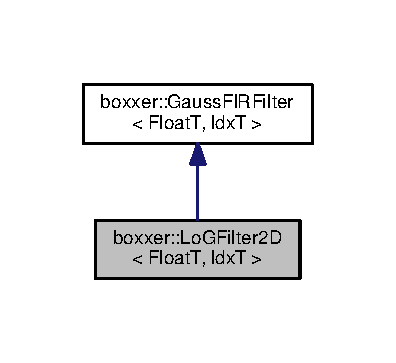
\includegraphics[width=190pt]{classboxxer_1_1LoGFilter2D__inherit__graph}
\end{center}
\end{figure}


Collaboration diagram for boxxer\+:\+:Lo\+G\+Filter2D$<$ FloatT, IdxT $>$\+:\nopagebreak
\begin{figure}[H]
\begin{center}
\leavevmode
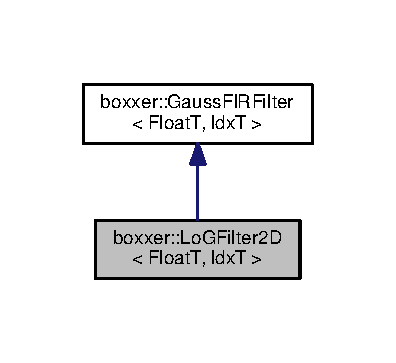
\includegraphics[width=190pt]{classboxxer_1_1LoGFilter2D__coll__graph}
\end{center}
\end{figure}
\subsubsection*{Public Types}
\begin{DoxyCompactItemize}
\item 
using \hyperlink{classboxxer_1_1LoGFilter2D_a14d26374dbb49a5e1cf43bb2257073ab}{I\+VecT} = typename \hyperlink{classboxxer_1_1GaussFIRFilter}{Gauss\+F\+I\+R\+Filter}$<$ FloatT, IdxT $>$\+::\hyperlink{classboxxer_1_1GaussFIRFilter_a0083c8c9ab6032dd458b4dc93852c2b8}{I\+VecT}
\item 
using \hyperlink{classboxxer_1_1LoGFilter2D_ac08d7bc8f4656f625c984a8a15db5e71}{VecT} = typename \hyperlink{classboxxer_1_1GaussFIRFilter}{Gauss\+F\+I\+R\+Filter}$<$ FloatT, IdxT $>$\+::\hyperlink{classboxxer_1_1LoGFilter2D_ac08d7bc8f4656f625c984a8a15db5e71}{VecT}
\item 
using \hyperlink{classboxxer_1_1LoGFilter2D_ad05a4ecfd5b16afe3a693bbd71a60425}{ImageT} = arma\+::\+Mat$<$ FloatT $>$
\item 
using \hyperlink{classboxxer_1_1GaussFIRFilter_a83cf4c7f4782f69918c0e0883fff5412}{MatT} = arma\+::\+Mat$<$ FloatT $>$
\end{DoxyCompactItemize}
\subsubsection*{Public Member Functions}
\begin{DoxyCompactItemize}
\item 
\hyperlink{classboxxer_1_1LoGFilter2D_a95dfb4584c05a63875b93724976e124f}{Lo\+G\+Filter2D} (const \hyperlink{classboxxer_1_1GaussFIRFilter_a0083c8c9ab6032dd458b4dc93852c2b8}{I\+VecT} \&\hyperlink{classboxxer_1_1GaussFIRFilter_ac0d4e19bb2be3e8913e77283e7e4317e}{size}, const \hyperlink{classboxxer_1_1LoGFilter2D_ac08d7bc8f4656f625c984a8a15db5e71}{VecT} \&\hyperlink{classboxxer_1_1GaussFIRFilter_a66ced06c688fd544d5f1f8be39aa2125}{sigma})
\item 
\hyperlink{classboxxer_1_1LoGFilter2D_afafdb9015e710e4d3df596e49aff2148}{Lo\+G\+Filter2D} (const \hyperlink{classboxxer_1_1GaussFIRFilter_a0083c8c9ab6032dd458b4dc93852c2b8}{I\+VecT} \&\hyperlink{classboxxer_1_1GaussFIRFilter_ac0d4e19bb2be3e8913e77283e7e4317e}{size}, const \hyperlink{classboxxer_1_1LoGFilter2D_ac08d7bc8f4656f625c984a8a15db5e71}{VecT} \&\hyperlink{classboxxer_1_1GaussFIRFilter_a66ced06c688fd544d5f1f8be39aa2125}{sigma}, const \hyperlink{classboxxer_1_1GaussFIRFilter_a0083c8c9ab6032dd458b4dc93852c2b8}{I\+VecT} \&kernel\+\_\+hw)
\item 
void \hyperlink{classboxxer_1_1LoGFilter2D_a21a9fc0913e13a1922cdda61ebf3cc1d}{set\+\_\+kernel\+\_\+hw} (const \hyperlink{classboxxer_1_1GaussFIRFilter_a0083c8c9ab6032dd458b4dc93852c2b8}{I\+VecT} \&kernel\+\_\+half\+\_\+width)
\item 
\hyperlink{classboxxer_1_1LoGFilter2D_ad05a4ecfd5b16afe3a693bbd71a60425}{ImageT} \hyperlink{classboxxer_1_1LoGFilter2D_ae3344ec82d3934c38893e1ad81dd71f9}{make\+\_\+image} () const 
\item 
void \hyperlink{classboxxer_1_1LoGFilter2D_a467ebae3f97f5f70c9760397b1163a46}{filter} (const \hyperlink{classboxxer_1_1LoGFilter2D_ad05a4ecfd5b16afe3a693bbd71a60425}{ImageT} \&im, \hyperlink{classboxxer_1_1LoGFilter2D_ad05a4ecfd5b16afe3a693bbd71a60425}{ImageT} \&out)
\item 
void \hyperlink{classboxxer_1_1LoGFilter2D_a8cfcad392f0e67302923b21301e88a7c}{test\+\_\+filter} (const \hyperlink{classboxxer_1_1LoGFilter2D_ad05a4ecfd5b16afe3a693bbd71a60425}{ImageT} \&im)
\end{DoxyCompactItemize}
\subsubsection*{Static Public Member Functions}
\begin{DoxyCompactItemize}
\item 
static \hyperlink{classboxxer_1_1LoGFilter2D_ac08d7bc8f4656f625c984a8a15db5e71}{VecT} \hyperlink{classboxxer_1_1GaussFIRFilter_a5dd6de5fe82092ec30141ab920d75dfd}{compute\+\_\+\+Gauss\+\_\+\+F\+I\+R\+\_\+kernel} (FloatT \hyperlink{classboxxer_1_1GaussFIRFilter_a66ced06c688fd544d5f1f8be39aa2125}{sigma}, IdxT \hyperlink{classboxxer_1_1GaussFIRFilter_ae17a4e137303e452a9223ba34825e0da}{hw})
\item 
static \hyperlink{classboxxer_1_1LoGFilter2D_ac08d7bc8f4656f625c984a8a15db5e71}{VecT} \hyperlink{classboxxer_1_1GaussFIRFilter_ad6a618b47db57b570278cc57b05d8c03}{compute\+\_\+\+Lo\+G\+\_\+\+F\+I\+R\+\_\+kernel} (FloatT \hyperlink{classboxxer_1_1GaussFIRFilter_a66ced06c688fd544d5f1f8be39aa2125}{sigma}, IdxT \hyperlink{classboxxer_1_1GaussFIRFilter_ae17a4e137303e452a9223ba34825e0da}{hw})
\end{DoxyCompactItemize}
\subsubsection*{Public Attributes}
\begin{DoxyCompactItemize}
\item 
IdxT \hyperlink{classboxxer_1_1GaussFIRFilter_ac7adcd4d8f8efee00a65262f596c8eda}{dim}
\item 
\hyperlink{classboxxer_1_1GaussFIRFilter_a0083c8c9ab6032dd458b4dc93852c2b8}{I\+VecT} \hyperlink{classboxxer_1_1GaussFIRFilter_ac0d4e19bb2be3e8913e77283e7e4317e}{size}
\item 
\hyperlink{classboxxer_1_1LoGFilter2D_ac08d7bc8f4656f625c984a8a15db5e71}{VecT} \hyperlink{classboxxer_1_1GaussFIRFilter_a66ced06c688fd544d5f1f8be39aa2125}{sigma}
\item 
\hyperlink{classboxxer_1_1GaussFIRFilter_a0083c8c9ab6032dd458b4dc93852c2b8}{I\+VecT} \hyperlink{classboxxer_1_1GaussFIRFilter_ae17a4e137303e452a9223ba34825e0da}{hw}
\end{DoxyCompactItemize}
\subsubsection*{Static Protected Attributes}
\begin{DoxyCompactItemize}
\item 
static const IdxT \hyperlink{classboxxer_1_1GaussFIRFilter_a7f85e018f78753ee4fedf65c04b0c65a}{max\+\_\+kernel\+\_\+hw}
\item 
static const FloatT \hyperlink{classboxxer_1_1GaussFIRFilter_a72b51cd7549510735179cb9c94f5f43f}{default\+\_\+sigma\+\_\+hw\+\_\+ratio}
\end{DoxyCompactItemize}
\subsubsection*{Friends}
\begin{DoxyCompactItemize}
\item 
{\footnotesize template$<$class Float\+T\+\_\+ , class Idx\+T\+\_\+ $>$ }\\std\+::ostream \& \hyperlink{classboxxer_1_1LoGFilter2D_acc81dcf998cd022738122bd24335c6a8}{operator$<$$<$} (std\+::ostream \&out, const \hyperlink{classboxxer_1_1LoGFilter2D}{Lo\+G\+Filter2D}$<$ Float\+T\+\_\+, Idx\+T\+\_\+ $>$ \&filt)
\end{DoxyCompactItemize}


\subsubsection{Detailed Description}
\subsubsection*{template$<$class FloatT = float, class IdxT = uint32\+\_\+t$>$\\*
class boxxer\+::\+Lo\+G\+Filter2\+D$<$ Float\+T, Idx\+T $>$}



Definition at line 98 of file Gauss\+Filter.\+h.



\subsubsection{Member Typedef Documentation}
\index{boxxer\+::\+Lo\+G\+Filter2D@{boxxer\+::\+Lo\+G\+Filter2D}!ImageT@{ImageT}}
\index{ImageT@{ImageT}!boxxer\+::\+Lo\+G\+Filter2D@{boxxer\+::\+Lo\+G\+Filter2D}}
\paragraph[{\texorpdfstring{ImageT}{ImageT}}]{\setlength{\rightskip}{0pt plus 5cm}template$<$class FloatT  = float, class IdxT  = uint32\+\_\+t$>$ using {\bf boxxer\+::\+Lo\+G\+Filter2D}$<$ FloatT, IdxT $>$\+::{\bf ImageT} =  arma\+::\+Mat$<$FloatT$>$}\hypertarget{classboxxer_1_1LoGFilter2D_ad05a4ecfd5b16afe3a693bbd71a60425}{}\label{classboxxer_1_1LoGFilter2D_ad05a4ecfd5b16afe3a693bbd71a60425}


Definition at line 103 of file Gauss\+Filter.\+h.

\index{boxxer\+::\+Lo\+G\+Filter2D@{boxxer\+::\+Lo\+G\+Filter2D}!I\+VecT@{I\+VecT}}
\index{I\+VecT@{I\+VecT}!boxxer\+::\+Lo\+G\+Filter2D@{boxxer\+::\+Lo\+G\+Filter2D}}
\paragraph[{\texorpdfstring{I\+VecT}{IVecT}}]{\setlength{\rightskip}{0pt plus 5cm}template$<$class FloatT  = float, class IdxT  = uint32\+\_\+t$>$ using {\bf boxxer\+::\+Lo\+G\+Filter2D}$<$ FloatT, IdxT $>$\+::{\bf I\+VecT} =  typename {\bf Gauss\+F\+I\+R\+Filter}$<$FloatT,IdxT$>$\+::{\bf I\+VecT}}\hypertarget{classboxxer_1_1LoGFilter2D_a14d26374dbb49a5e1cf43bb2257073ab}{}\label{classboxxer_1_1LoGFilter2D_a14d26374dbb49a5e1cf43bb2257073ab}


Definition at line 101 of file Gauss\+Filter.\+h.

\index{boxxer\+::\+Lo\+G\+Filter2D@{boxxer\+::\+Lo\+G\+Filter2D}!MatT@{MatT}}
\index{MatT@{MatT}!boxxer\+::\+Lo\+G\+Filter2D@{boxxer\+::\+Lo\+G\+Filter2D}}
\paragraph[{\texorpdfstring{MatT}{MatT}}]{\setlength{\rightskip}{0pt plus 5cm}template$<$class FloatT = float, class IdxT = uint32\+\_\+t$>$ using {\bf boxxer\+::\+Gauss\+F\+I\+R\+Filter}$<$ FloatT, IdxT $>$\+::{\bf MatT} =  arma\+::\+Mat$<$FloatT$>$\hspace{0.3cm}{\ttfamily [inherited]}}\hypertarget{classboxxer_1_1GaussFIRFilter_a83cf4c7f4782f69918c0e0883fff5412}{}\label{classboxxer_1_1GaussFIRFilter_a83cf4c7f4782f69918c0e0883fff5412}


Definition at line 26 of file Gauss\+Filter.\+h.

\index{boxxer\+::\+Lo\+G\+Filter2D@{boxxer\+::\+Lo\+G\+Filter2D}!VecT@{VecT}}
\index{VecT@{VecT}!boxxer\+::\+Lo\+G\+Filter2D@{boxxer\+::\+Lo\+G\+Filter2D}}
\paragraph[{\texorpdfstring{VecT}{VecT}}]{\setlength{\rightskip}{0pt plus 5cm}template$<$class FloatT  = float, class IdxT  = uint32\+\_\+t$>$ using {\bf boxxer\+::\+Lo\+G\+Filter2D}$<$ FloatT, IdxT $>$\+::{\bf VecT} =  typename {\bf Gauss\+F\+I\+R\+Filter}$<$FloatT,IdxT$>$\+::{\bf VecT}}\hypertarget{classboxxer_1_1LoGFilter2D_ac08d7bc8f4656f625c984a8a15db5e71}{}\label{classboxxer_1_1LoGFilter2D_ac08d7bc8f4656f625c984a8a15db5e71}


Definition at line 102 of file Gauss\+Filter.\+h.



\subsubsection{Constructor \& Destructor Documentation}
\index{boxxer\+::\+Lo\+G\+Filter2D@{boxxer\+::\+Lo\+G\+Filter2D}!Lo\+G\+Filter2D@{Lo\+G\+Filter2D}}
\index{Lo\+G\+Filter2D@{Lo\+G\+Filter2D}!boxxer\+::\+Lo\+G\+Filter2D@{boxxer\+::\+Lo\+G\+Filter2D}}
\paragraph[{\texorpdfstring{Lo\+G\+Filter2\+D(const I\+Vec\+T \&size, const Vec\+T \&sigma)}{LoGFilter2D(const IVecT &size, const VecT &sigma)}}]{\setlength{\rightskip}{0pt plus 5cm}template$<$class FloatT  = float, class IdxT  = uint32\+\_\+t$>$ {\bf boxxer\+::\+Lo\+G\+Filter2D}$<$ FloatT, IdxT $>$\+::{\bf Lo\+G\+Filter2D} (
\begin{DoxyParamCaption}
\item[{const {\bf I\+VecT} \&}]{size, }
\item[{const {\bf VecT} \&}]{sigma}
\end{DoxyParamCaption}
)}\hypertarget{classboxxer_1_1LoGFilter2D_a95dfb4584c05a63875b93724976e124f}{}\label{classboxxer_1_1LoGFilter2D_a95dfb4584c05a63875b93724976e124f}
\index{boxxer\+::\+Lo\+G\+Filter2D@{boxxer\+::\+Lo\+G\+Filter2D}!Lo\+G\+Filter2D@{Lo\+G\+Filter2D}}
\index{Lo\+G\+Filter2D@{Lo\+G\+Filter2D}!boxxer\+::\+Lo\+G\+Filter2D@{boxxer\+::\+Lo\+G\+Filter2D}}
\paragraph[{\texorpdfstring{Lo\+G\+Filter2\+D(const I\+Vec\+T \&size, const Vec\+T \&sigma, const I\+Vec\+T \&kernel\+\_\+hw)}{LoGFilter2D(const IVecT &size, const VecT &sigma, const IVecT &kernel_hw)}}]{\setlength{\rightskip}{0pt plus 5cm}template$<$class FloatT  = float, class IdxT  = uint32\+\_\+t$>$ {\bf boxxer\+::\+Lo\+G\+Filter2D}$<$ FloatT, IdxT $>$\+::{\bf Lo\+G\+Filter2D} (
\begin{DoxyParamCaption}
\item[{const {\bf I\+VecT} \&}]{size, }
\item[{const {\bf VecT} \&}]{sigma, }
\item[{const {\bf I\+VecT} \&}]{kernel\+\_\+hw}
\end{DoxyParamCaption}
)}\hypertarget{classboxxer_1_1LoGFilter2D_afafdb9015e710e4d3df596e49aff2148}{}\label{classboxxer_1_1LoGFilter2D_afafdb9015e710e4d3df596e49aff2148}


\subsubsection{Member Function Documentation}
\index{boxxer\+::\+Lo\+G\+Filter2D@{boxxer\+::\+Lo\+G\+Filter2D}!compute\+\_\+\+Gauss\+\_\+\+F\+I\+R\+\_\+kernel@{compute\+\_\+\+Gauss\+\_\+\+F\+I\+R\+\_\+kernel}}
\index{compute\+\_\+\+Gauss\+\_\+\+F\+I\+R\+\_\+kernel@{compute\+\_\+\+Gauss\+\_\+\+F\+I\+R\+\_\+kernel}!boxxer\+::\+Lo\+G\+Filter2D@{boxxer\+::\+Lo\+G\+Filter2D}}
\paragraph[{\texorpdfstring{compute\+\_\+\+Gauss\+\_\+\+F\+I\+R\+\_\+kernel(\+Float\+T sigma, Idx\+T hw)}{compute_Gauss_FIR_kernel(FloatT sigma, IdxT hw)}}]{\setlength{\rightskip}{0pt plus 5cm}template$<$class FloatT = float, class IdxT = uint32\+\_\+t$>$ static {\bf VecT} {\bf boxxer\+::\+Gauss\+F\+I\+R\+Filter}$<$ FloatT, IdxT $>$\+::compute\+\_\+\+Gauss\+\_\+\+F\+I\+R\+\_\+kernel (
\begin{DoxyParamCaption}
\item[{FloatT}]{sigma, }
\item[{IdxT}]{hw}
\end{DoxyParamCaption}
)\hspace{0.3cm}{\ttfamily [static]}, {\ttfamily [inherited]}}\hypertarget{classboxxer_1_1GaussFIRFilter_a5dd6de5fe82092ec30141ab920d75dfd}{}\label{classboxxer_1_1GaussFIRFilter_a5dd6de5fe82092ec30141ab920d75dfd}
\index{boxxer\+::\+Lo\+G\+Filter2D@{boxxer\+::\+Lo\+G\+Filter2D}!compute\+\_\+\+Lo\+G\+\_\+\+F\+I\+R\+\_\+kernel@{compute\+\_\+\+Lo\+G\+\_\+\+F\+I\+R\+\_\+kernel}}
\index{compute\+\_\+\+Lo\+G\+\_\+\+F\+I\+R\+\_\+kernel@{compute\+\_\+\+Lo\+G\+\_\+\+F\+I\+R\+\_\+kernel}!boxxer\+::\+Lo\+G\+Filter2D@{boxxer\+::\+Lo\+G\+Filter2D}}
\paragraph[{\texorpdfstring{compute\+\_\+\+Lo\+G\+\_\+\+F\+I\+R\+\_\+kernel(\+Float\+T sigma, Idx\+T hw)}{compute_LoG_FIR_kernel(FloatT sigma, IdxT hw)}}]{\setlength{\rightskip}{0pt plus 5cm}template$<$class FloatT = float, class IdxT = uint32\+\_\+t$>$ static {\bf VecT} {\bf boxxer\+::\+Gauss\+F\+I\+R\+Filter}$<$ FloatT, IdxT $>$\+::compute\+\_\+\+Lo\+G\+\_\+\+F\+I\+R\+\_\+kernel (
\begin{DoxyParamCaption}
\item[{FloatT}]{sigma, }
\item[{IdxT}]{hw}
\end{DoxyParamCaption}
)\hspace{0.3cm}{\ttfamily [static]}, {\ttfamily [inherited]}}\hypertarget{classboxxer_1_1GaussFIRFilter_ad6a618b47db57b570278cc57b05d8c03}{}\label{classboxxer_1_1GaussFIRFilter_ad6a618b47db57b570278cc57b05d8c03}
\index{boxxer\+::\+Lo\+G\+Filter2D@{boxxer\+::\+Lo\+G\+Filter2D}!filter@{filter}}
\index{filter@{filter}!boxxer\+::\+Lo\+G\+Filter2D@{boxxer\+::\+Lo\+G\+Filter2D}}
\paragraph[{\texorpdfstring{filter(const Image\+T \&im, Image\+T \&out)}{filter(const ImageT &im, ImageT &out)}}]{\setlength{\rightskip}{0pt plus 5cm}template$<$class FloatT  = float, class IdxT  = uint32\+\_\+t$>$ void {\bf boxxer\+::\+Lo\+G\+Filter2D}$<$ FloatT, IdxT $>$\+::filter (
\begin{DoxyParamCaption}
\item[{const {\bf ImageT} \&}]{im, }
\item[{{\bf ImageT} \&}]{out}
\end{DoxyParamCaption}
)}\hypertarget{classboxxer_1_1LoGFilter2D_a467ebae3f97f5f70c9760397b1163a46}{}\label{classboxxer_1_1LoGFilter2D_a467ebae3f97f5f70c9760397b1163a46}
\index{boxxer\+::\+Lo\+G\+Filter2D@{boxxer\+::\+Lo\+G\+Filter2D}!make\+\_\+image@{make\+\_\+image}}
\index{make\+\_\+image@{make\+\_\+image}!boxxer\+::\+Lo\+G\+Filter2D@{boxxer\+::\+Lo\+G\+Filter2D}}
\paragraph[{\texorpdfstring{make\+\_\+image() const }{make_image() const }}]{\setlength{\rightskip}{0pt plus 5cm}template$<$class FloatT  = float, class IdxT  = uint32\+\_\+t$>$ {\bf ImageT} {\bf boxxer\+::\+Lo\+G\+Filter2D}$<$ FloatT, IdxT $>$\+::make\+\_\+image (
\begin{DoxyParamCaption}
{}
\end{DoxyParamCaption}
) const\hspace{0.3cm}{\ttfamily [inline]}}\hypertarget{classboxxer_1_1LoGFilter2D_ae3344ec82d3934c38893e1ad81dd71f9}{}\label{classboxxer_1_1LoGFilter2D_ae3344ec82d3934c38893e1ad81dd71f9}


Definition at line 108 of file Gauss\+Filter.\+h.



References boxxer\+::\+Gauss\+F\+I\+R\+Filter$<$ Float\+T, Idx\+T $>$\+::size.

\index{boxxer\+::\+Lo\+G\+Filter2D@{boxxer\+::\+Lo\+G\+Filter2D}!set\+\_\+kernel\+\_\+hw@{set\+\_\+kernel\+\_\+hw}}
\index{set\+\_\+kernel\+\_\+hw@{set\+\_\+kernel\+\_\+hw}!boxxer\+::\+Lo\+G\+Filter2D@{boxxer\+::\+Lo\+G\+Filter2D}}
\paragraph[{\texorpdfstring{set\+\_\+kernel\+\_\+hw(const I\+Vec\+T \&kernel\+\_\+half\+\_\+width)}{set_kernel_hw(const IVecT &kernel_half_width)}}]{\setlength{\rightskip}{0pt plus 5cm}template$<$class FloatT  = float, class IdxT  = uint32\+\_\+t$>$ void {\bf boxxer\+::\+Lo\+G\+Filter2D}$<$ FloatT, IdxT $>$\+::set\+\_\+kernel\+\_\+hw (
\begin{DoxyParamCaption}
\item[{const {\bf I\+VecT} \&}]{kernel\+\_\+half\+\_\+width}
\end{DoxyParamCaption}
)\hspace{0.3cm}{\ttfamily [virtual]}}\hypertarget{classboxxer_1_1LoGFilter2D_a21a9fc0913e13a1922cdda61ebf3cc1d}{}\label{classboxxer_1_1LoGFilter2D_a21a9fc0913e13a1922cdda61ebf3cc1d}


Implements \hyperlink{classboxxer_1_1GaussFIRFilter_a7ada113680b67f052d11afe346ddf8bc}{boxxer\+::\+Gauss\+F\+I\+R\+Filter$<$ Float\+T, Idx\+T $>$}.

\index{boxxer\+::\+Lo\+G\+Filter2D@{boxxer\+::\+Lo\+G\+Filter2D}!test\+\_\+filter@{test\+\_\+filter}}
\index{test\+\_\+filter@{test\+\_\+filter}!boxxer\+::\+Lo\+G\+Filter2D@{boxxer\+::\+Lo\+G\+Filter2D}}
\paragraph[{\texorpdfstring{test\+\_\+filter(const Image\+T \&im)}{test_filter(const ImageT &im)}}]{\setlength{\rightskip}{0pt plus 5cm}template$<$class FloatT  = float, class IdxT  = uint32\+\_\+t$>$ void {\bf boxxer\+::\+Lo\+G\+Filter2D}$<$ FloatT, IdxT $>$\+::test\+\_\+filter (
\begin{DoxyParamCaption}
\item[{const {\bf ImageT} \&}]{im}
\end{DoxyParamCaption}
)}\hypertarget{classboxxer_1_1LoGFilter2D_a8cfcad392f0e67302923b21301e88a7c}{}\label{classboxxer_1_1LoGFilter2D_a8cfcad392f0e67302923b21301e88a7c}


\subsubsection{Friends And Related Function Documentation}
\index{boxxer\+::\+Lo\+G\+Filter2D@{boxxer\+::\+Lo\+G\+Filter2D}!operator$<$$<$@{operator$<$$<$}}
\index{operator$<$$<$@{operator$<$$<$}!boxxer\+::\+Lo\+G\+Filter2D@{boxxer\+::\+Lo\+G\+Filter2D}}
\paragraph[{\texorpdfstring{operator$<$$<$}{operator<<}}]{\setlength{\rightskip}{0pt plus 5cm}template$<$class FloatT  = float, class IdxT  = uint32\+\_\+t$>$ template$<$class Float\+T\+\_\+ , class Idx\+T\+\_\+ $>$ std\+::ostream\& operator$<$$<$ (
\begin{DoxyParamCaption}
\item[{std\+::ostream \&}]{out, }
\item[{const {\bf Lo\+G\+Filter2D}$<$ Float\+T\+\_\+, Idx\+T\+\_\+ $>$ \&}]{filt}
\end{DoxyParamCaption}
)\hspace{0.3cm}{\ttfamily [friend]}}\hypertarget{classboxxer_1_1LoGFilter2D_acc81dcf998cd022738122bd24335c6a8}{}\label{classboxxer_1_1LoGFilter2D_acc81dcf998cd022738122bd24335c6a8}


\subsubsection{Member Data Documentation}
\index{boxxer\+::\+Lo\+G\+Filter2D@{boxxer\+::\+Lo\+G\+Filter2D}!default\+\_\+sigma\+\_\+hw\+\_\+ratio@{default\+\_\+sigma\+\_\+hw\+\_\+ratio}}
\index{default\+\_\+sigma\+\_\+hw\+\_\+ratio@{default\+\_\+sigma\+\_\+hw\+\_\+ratio}!boxxer\+::\+Lo\+G\+Filter2D@{boxxer\+::\+Lo\+G\+Filter2D}}
\paragraph[{\texorpdfstring{default\+\_\+sigma\+\_\+hw\+\_\+ratio}{default_sigma_hw_ratio}}]{\setlength{\rightskip}{0pt plus 5cm}template$<$class FloatT = float, class IdxT = uint32\+\_\+t$>$ const FloatT {\bf boxxer\+::\+Gauss\+F\+I\+R\+Filter}$<$ FloatT, IdxT $>$\+::default\+\_\+sigma\+\_\+hw\+\_\+ratio\hspace{0.3cm}{\ttfamily [static]}, {\ttfamily [protected]}, {\ttfamily [inherited]}}\hypertarget{classboxxer_1_1GaussFIRFilter_a72b51cd7549510735179cb9c94f5f43f}{}\label{classboxxer_1_1GaussFIRFilter_a72b51cd7549510735179cb9c94f5f43f}


Definition at line 41 of file Gauss\+Filter.\+h.

\index{boxxer\+::\+Lo\+G\+Filter2D@{boxxer\+::\+Lo\+G\+Filter2D}!dim@{dim}}
\index{dim@{dim}!boxxer\+::\+Lo\+G\+Filter2D@{boxxer\+::\+Lo\+G\+Filter2D}}
\paragraph[{\texorpdfstring{dim}{dim}}]{\setlength{\rightskip}{0pt plus 5cm}template$<$class FloatT = float, class IdxT = uint32\+\_\+t$>$ IdxT {\bf boxxer\+::\+Gauss\+F\+I\+R\+Filter}$<$ FloatT, IdxT $>$\+::dim\hspace{0.3cm}{\ttfamily [inherited]}}\hypertarget{classboxxer_1_1GaussFIRFilter_ac7adcd4d8f8efee00a65262f596c8eda}{}\label{classboxxer_1_1GaussFIRFilter_ac7adcd4d8f8efee00a65262f596c8eda}


Definition at line 28 of file Gauss\+Filter.\+h.

\index{boxxer\+::\+Lo\+G\+Filter2D@{boxxer\+::\+Lo\+G\+Filter2D}!hw@{hw}}
\index{hw@{hw}!boxxer\+::\+Lo\+G\+Filter2D@{boxxer\+::\+Lo\+G\+Filter2D}}
\paragraph[{\texorpdfstring{hw}{hw}}]{\setlength{\rightskip}{0pt plus 5cm}template$<$class FloatT = float, class IdxT = uint32\+\_\+t$>$ {\bf I\+VecT} {\bf boxxer\+::\+Gauss\+F\+I\+R\+Filter}$<$ FloatT, IdxT $>$\+::hw\hspace{0.3cm}{\ttfamily [inherited]}}\hypertarget{classboxxer_1_1GaussFIRFilter_ae17a4e137303e452a9223ba34825e0da}{}\label{classboxxer_1_1GaussFIRFilter_ae17a4e137303e452a9223ba34825e0da}


Definition at line 31 of file Gauss\+Filter.\+h.

\index{boxxer\+::\+Lo\+G\+Filter2D@{boxxer\+::\+Lo\+G\+Filter2D}!max\+\_\+kernel\+\_\+hw@{max\+\_\+kernel\+\_\+hw}}
\index{max\+\_\+kernel\+\_\+hw@{max\+\_\+kernel\+\_\+hw}!boxxer\+::\+Lo\+G\+Filter2D@{boxxer\+::\+Lo\+G\+Filter2D}}
\paragraph[{\texorpdfstring{max\+\_\+kernel\+\_\+hw}{max_kernel_hw}}]{\setlength{\rightskip}{0pt plus 5cm}template$<$class FloatT = float, class IdxT = uint32\+\_\+t$>$ const IdxT {\bf boxxer\+::\+Gauss\+F\+I\+R\+Filter}$<$ FloatT, IdxT $>$\+::max\+\_\+kernel\+\_\+hw\hspace{0.3cm}{\ttfamily [static]}, {\ttfamily [protected]}, {\ttfamily [inherited]}}\hypertarget{classboxxer_1_1GaussFIRFilter_a7f85e018f78753ee4fedf65c04b0c65a}{}\label{classboxxer_1_1GaussFIRFilter_a7f85e018f78753ee4fedf65c04b0c65a}


Definition at line 40 of file Gauss\+Filter.\+h.

\index{boxxer\+::\+Lo\+G\+Filter2D@{boxxer\+::\+Lo\+G\+Filter2D}!sigma@{sigma}}
\index{sigma@{sigma}!boxxer\+::\+Lo\+G\+Filter2D@{boxxer\+::\+Lo\+G\+Filter2D}}
\paragraph[{\texorpdfstring{sigma}{sigma}}]{\setlength{\rightskip}{0pt plus 5cm}template$<$class FloatT = float, class IdxT = uint32\+\_\+t$>$ {\bf VecT} {\bf boxxer\+::\+Gauss\+F\+I\+R\+Filter}$<$ FloatT, IdxT $>$\+::sigma\hspace{0.3cm}{\ttfamily [inherited]}}\hypertarget{classboxxer_1_1GaussFIRFilter_a66ced06c688fd544d5f1f8be39aa2125}{}\label{classboxxer_1_1GaussFIRFilter_a66ced06c688fd544d5f1f8be39aa2125}


Definition at line 30 of file Gauss\+Filter.\+h.

\index{boxxer\+::\+Lo\+G\+Filter2D@{boxxer\+::\+Lo\+G\+Filter2D}!size@{size}}
\index{size@{size}!boxxer\+::\+Lo\+G\+Filter2D@{boxxer\+::\+Lo\+G\+Filter2D}}
\paragraph[{\texorpdfstring{size}{size}}]{\setlength{\rightskip}{0pt plus 5cm}template$<$class FloatT = float, class IdxT = uint32\+\_\+t$>$ {\bf I\+VecT} {\bf boxxer\+::\+Gauss\+F\+I\+R\+Filter}$<$ FloatT, IdxT $>$\+::size\hspace{0.3cm}{\ttfamily [inherited]}}\hypertarget{classboxxer_1_1GaussFIRFilter_ac0d4e19bb2be3e8913e77283e7e4317e}{}\label{classboxxer_1_1GaussFIRFilter_ac0d4e19bb2be3e8913e77283e7e4317e}


Definition at line 29 of file Gauss\+Filter.\+h.



Referenced by boxxer\+::\+Gauss\+Filter2\+D$<$ Float\+T, Idx\+T $>$\+::make\+\_\+image(), boxxer\+::\+Do\+G\+Filter2\+D$<$ Float\+T, Idx\+T $>$\+::make\+\_\+image(), boxxer\+::\+Lo\+G\+Filter2\+D$<$ Float\+T, Idx\+T $>$\+::make\+\_\+image(), boxxer\+::\+Gauss\+Filter3\+D$<$ Float\+T, Idx\+T $>$\+::make\+\_\+image(), boxxer\+::\+Do\+G\+Filter3\+D$<$ Float\+T, Idx\+T $>$\+::make\+\_\+image(), and boxxer\+::\+Lo\+G\+Filter3\+D$<$ Float\+T, Idx\+T $>$\+::make\+\_\+image().



The documentation for this class was generated from the following file\+:\begin{DoxyCompactItemize}
\item 
\hyperlink{GaussFilter_8h}{Gauss\+Filter.\+h}\end{DoxyCompactItemize}

\hypertarget{classboxxer_1_1LoGFilter3D}{}\subsection{boxxer\+:\+:Lo\+G\+Filter3D$<$ FloatT, IdxT $>$ Class Template Reference}
\label{classboxxer_1_1LoGFilter3D}\index{boxxer\+::\+Lo\+G\+Filter3\+D$<$ Float\+T, Idx\+T $>$@{boxxer\+::\+Lo\+G\+Filter3\+D$<$ Float\+T, Idx\+T $>$}}


{\ttfamily \#include $<$/home/travis/build/markjolah/\+Boxxer/include/\+Boxxer/\+Gauss\+Filter.\+h$>$}



Inheritance diagram for boxxer\+:\+:Lo\+G\+Filter3D$<$ FloatT, IdxT $>$\+:\nopagebreak
\begin{figure}[H]
\begin{center}
\leavevmode
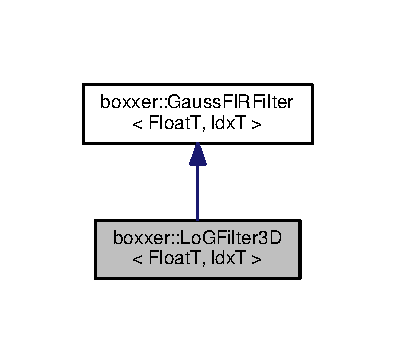
\includegraphics[width=190pt]{classboxxer_1_1LoGFilter3D__inherit__graph}
\end{center}
\end{figure}


Collaboration diagram for boxxer\+:\+:Lo\+G\+Filter3D$<$ FloatT, IdxT $>$\+:\nopagebreak
\begin{figure}[H]
\begin{center}
\leavevmode
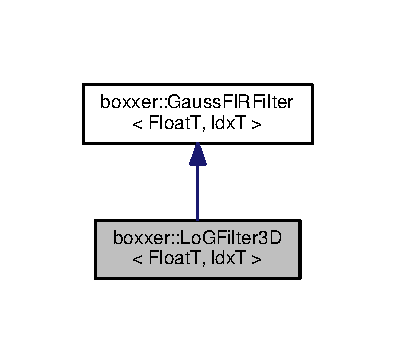
\includegraphics[width=190pt]{classboxxer_1_1LoGFilter3D__coll__graph}
\end{center}
\end{figure}
\subsubsection*{Public Types}
\begin{DoxyCompactItemize}
\item 
using \hyperlink{classboxxer_1_1LoGFilter3D_a7471a6baf4e07f70d6ba8100bf90b1a2}{I\+VecT} = typename \hyperlink{classboxxer_1_1GaussFIRFilter}{Gauss\+F\+I\+R\+Filter}$<$ FloatT, IdxT $>$\+::\hyperlink{classboxxer_1_1GaussFIRFilter_a0083c8c9ab6032dd458b4dc93852c2b8}{I\+VecT}
\item 
using \hyperlink{classboxxer_1_1LoGFilter3D_ad4ce9fa2ad4134b954162e2597fb6a48}{VecT} = typename \hyperlink{classboxxer_1_1GaussFIRFilter}{Gauss\+F\+I\+R\+Filter}$<$ FloatT, IdxT $>$\+::\hyperlink{classboxxer_1_1LoGFilter3D_ad4ce9fa2ad4134b954162e2597fb6a48}{VecT}
\item 
using \hyperlink{classboxxer_1_1LoGFilter3D_a735a23ffea030e730398d32a49d2b223}{ImageT} = arma\+::\+Cube$<$ FloatT $>$
\item 
using \hyperlink{classboxxer_1_1GaussFIRFilter_a83cf4c7f4782f69918c0e0883fff5412}{MatT} = arma\+::\+Mat$<$ FloatT $>$
\end{DoxyCompactItemize}
\subsubsection*{Public Member Functions}
\begin{DoxyCompactItemize}
\item 
\hyperlink{classboxxer_1_1LoGFilter3D_a84c56c8dbaec1a442e061f1d54ed1981}{Lo\+G\+Filter3D} (const \hyperlink{classboxxer_1_1GaussFIRFilter_a0083c8c9ab6032dd458b4dc93852c2b8}{I\+VecT} \&\hyperlink{classboxxer_1_1GaussFIRFilter_ac0d4e19bb2be3e8913e77283e7e4317e}{size}, const \hyperlink{classboxxer_1_1LoGFilter3D_ad4ce9fa2ad4134b954162e2597fb6a48}{VecT} \&\hyperlink{classboxxer_1_1GaussFIRFilter_a66ced06c688fd544d5f1f8be39aa2125}{sigma})
\item 
\hyperlink{classboxxer_1_1LoGFilter3D_a1a855e4acb2ad962eb80e5dfa4e764e4}{Lo\+G\+Filter3D} (const \hyperlink{classboxxer_1_1GaussFIRFilter_a0083c8c9ab6032dd458b4dc93852c2b8}{I\+VecT} \&\hyperlink{classboxxer_1_1GaussFIRFilter_ac0d4e19bb2be3e8913e77283e7e4317e}{size}, const \hyperlink{classboxxer_1_1LoGFilter3D_ad4ce9fa2ad4134b954162e2597fb6a48}{VecT} \&\hyperlink{classboxxer_1_1GaussFIRFilter_a66ced06c688fd544d5f1f8be39aa2125}{sigma}, const \hyperlink{classboxxer_1_1GaussFIRFilter_a0083c8c9ab6032dd458b4dc93852c2b8}{I\+VecT} \&kernel\+\_\+hw)
\item 
void \hyperlink{classboxxer_1_1LoGFilter3D_ab7b66d1b3262dfe6033ab58d9221f7e2}{set\+\_\+kernel\+\_\+hw} (const \hyperlink{classboxxer_1_1GaussFIRFilter_a0083c8c9ab6032dd458b4dc93852c2b8}{I\+VecT} \&kernel\+\_\+half\+\_\+width)
\item 
\hyperlink{classboxxer_1_1LoGFilter3D_a735a23ffea030e730398d32a49d2b223}{ImageT} \hyperlink{classboxxer_1_1LoGFilter3D_a0c7867d14ded5d7bda15dae3e207e69d}{make\+\_\+image} () const 
\item 
void \hyperlink{classboxxer_1_1LoGFilter3D_ab28a7d1e2e8a4af00a05810922a6c54f}{filter} (const \hyperlink{classboxxer_1_1LoGFilter3D_a735a23ffea030e730398d32a49d2b223}{ImageT} \&im, \hyperlink{classboxxer_1_1LoGFilter3D_a735a23ffea030e730398d32a49d2b223}{ImageT} \&out)
\item 
void \hyperlink{classboxxer_1_1LoGFilter3D_a11358de783c69458a79baaa3c688be93}{test\+\_\+filter} (const \hyperlink{classboxxer_1_1LoGFilter3D_a735a23ffea030e730398d32a49d2b223}{ImageT} \&im)
\end{DoxyCompactItemize}
\subsubsection*{Static Public Member Functions}
\begin{DoxyCompactItemize}
\item 
static \hyperlink{classboxxer_1_1LoGFilter3D_ad4ce9fa2ad4134b954162e2597fb6a48}{VecT} \hyperlink{classboxxer_1_1GaussFIRFilter_a5dd6de5fe82092ec30141ab920d75dfd}{compute\+\_\+\+Gauss\+\_\+\+F\+I\+R\+\_\+kernel} (FloatT \hyperlink{classboxxer_1_1GaussFIRFilter_a66ced06c688fd544d5f1f8be39aa2125}{sigma}, IdxT \hyperlink{classboxxer_1_1GaussFIRFilter_ae17a4e137303e452a9223ba34825e0da}{hw})
\item 
static \hyperlink{classboxxer_1_1LoGFilter3D_ad4ce9fa2ad4134b954162e2597fb6a48}{VecT} \hyperlink{classboxxer_1_1GaussFIRFilter_ad6a618b47db57b570278cc57b05d8c03}{compute\+\_\+\+Lo\+G\+\_\+\+F\+I\+R\+\_\+kernel} (FloatT \hyperlink{classboxxer_1_1GaussFIRFilter_a66ced06c688fd544d5f1f8be39aa2125}{sigma}, IdxT \hyperlink{classboxxer_1_1GaussFIRFilter_ae17a4e137303e452a9223ba34825e0da}{hw})
\end{DoxyCompactItemize}
\subsubsection*{Public Attributes}
\begin{DoxyCompactItemize}
\item 
IdxT \hyperlink{classboxxer_1_1GaussFIRFilter_ac7adcd4d8f8efee00a65262f596c8eda}{dim}
\item 
\hyperlink{classboxxer_1_1GaussFIRFilter_a0083c8c9ab6032dd458b4dc93852c2b8}{I\+VecT} \hyperlink{classboxxer_1_1GaussFIRFilter_ac0d4e19bb2be3e8913e77283e7e4317e}{size}
\item 
\hyperlink{classboxxer_1_1LoGFilter3D_ad4ce9fa2ad4134b954162e2597fb6a48}{VecT} \hyperlink{classboxxer_1_1GaussFIRFilter_a66ced06c688fd544d5f1f8be39aa2125}{sigma}
\item 
\hyperlink{classboxxer_1_1GaussFIRFilter_a0083c8c9ab6032dd458b4dc93852c2b8}{I\+VecT} \hyperlink{classboxxer_1_1GaussFIRFilter_ae17a4e137303e452a9223ba34825e0da}{hw}
\end{DoxyCompactItemize}
\subsubsection*{Static Protected Attributes}
\begin{DoxyCompactItemize}
\item 
static const IdxT \hyperlink{classboxxer_1_1GaussFIRFilter_a7f85e018f78753ee4fedf65c04b0c65a}{max\+\_\+kernel\+\_\+hw}
\item 
static const FloatT \hyperlink{classboxxer_1_1GaussFIRFilter_a72b51cd7549510735179cb9c94f5f43f}{default\+\_\+sigma\+\_\+hw\+\_\+ratio}
\end{DoxyCompactItemize}
\subsubsection*{Friends}
\begin{DoxyCompactItemize}
\item 
{\footnotesize template$<$class Float\+T\+\_\+ , class Idx\+T\+\_\+ $>$ }\\std\+::ostream \& \hyperlink{classboxxer_1_1LoGFilter3D_ae45bb5dbe9dc918aaaa8b484f5d63ce5}{operator$<$$<$} (std\+::ostream \&out, const \hyperlink{classboxxer_1_1LoGFilter3D}{Lo\+G\+Filter3D}$<$ Float\+T\+\_\+, Idx\+T\+\_\+ $>$ \&filt)
\end{DoxyCompactItemize}


\subsubsection{Detailed Description}
\subsubsection*{template$<$class FloatT = float, class IdxT = uint32\+\_\+t$>$\\*
class boxxer\+::\+Lo\+G\+Filter3\+D$<$ Float\+T, Idx\+T $>$}



Definition at line 178 of file Gauss\+Filter.\+h.



\subsubsection{Member Typedef Documentation}
\index{boxxer\+::\+Lo\+G\+Filter3D@{boxxer\+::\+Lo\+G\+Filter3D}!ImageT@{ImageT}}
\index{ImageT@{ImageT}!boxxer\+::\+Lo\+G\+Filter3D@{boxxer\+::\+Lo\+G\+Filter3D}}
\paragraph[{\texorpdfstring{ImageT}{ImageT}}]{\setlength{\rightskip}{0pt plus 5cm}template$<$class FloatT  = float, class IdxT  = uint32\+\_\+t$>$ using {\bf boxxer\+::\+Lo\+G\+Filter3D}$<$ FloatT, IdxT $>$\+::{\bf ImageT} =  arma\+::\+Cube$<$FloatT$>$}\hypertarget{classboxxer_1_1LoGFilter3D_a735a23ffea030e730398d32a49d2b223}{}\label{classboxxer_1_1LoGFilter3D_a735a23ffea030e730398d32a49d2b223}


Definition at line 183 of file Gauss\+Filter.\+h.

\index{boxxer\+::\+Lo\+G\+Filter3D@{boxxer\+::\+Lo\+G\+Filter3D}!I\+VecT@{I\+VecT}}
\index{I\+VecT@{I\+VecT}!boxxer\+::\+Lo\+G\+Filter3D@{boxxer\+::\+Lo\+G\+Filter3D}}
\paragraph[{\texorpdfstring{I\+VecT}{IVecT}}]{\setlength{\rightskip}{0pt plus 5cm}template$<$class FloatT  = float, class IdxT  = uint32\+\_\+t$>$ using {\bf boxxer\+::\+Lo\+G\+Filter3D}$<$ FloatT, IdxT $>$\+::{\bf I\+VecT} =  typename {\bf Gauss\+F\+I\+R\+Filter}$<$FloatT,IdxT$>$\+::{\bf I\+VecT}}\hypertarget{classboxxer_1_1LoGFilter3D_a7471a6baf4e07f70d6ba8100bf90b1a2}{}\label{classboxxer_1_1LoGFilter3D_a7471a6baf4e07f70d6ba8100bf90b1a2}


Definition at line 181 of file Gauss\+Filter.\+h.

\index{boxxer\+::\+Lo\+G\+Filter3D@{boxxer\+::\+Lo\+G\+Filter3D}!MatT@{MatT}}
\index{MatT@{MatT}!boxxer\+::\+Lo\+G\+Filter3D@{boxxer\+::\+Lo\+G\+Filter3D}}
\paragraph[{\texorpdfstring{MatT}{MatT}}]{\setlength{\rightskip}{0pt plus 5cm}template$<$class FloatT = float, class IdxT = uint32\+\_\+t$>$ using {\bf boxxer\+::\+Gauss\+F\+I\+R\+Filter}$<$ FloatT, IdxT $>$\+::{\bf MatT} =  arma\+::\+Mat$<$FloatT$>$\hspace{0.3cm}{\ttfamily [inherited]}}\hypertarget{classboxxer_1_1GaussFIRFilter_a83cf4c7f4782f69918c0e0883fff5412}{}\label{classboxxer_1_1GaussFIRFilter_a83cf4c7f4782f69918c0e0883fff5412}


Definition at line 26 of file Gauss\+Filter.\+h.

\index{boxxer\+::\+Lo\+G\+Filter3D@{boxxer\+::\+Lo\+G\+Filter3D}!VecT@{VecT}}
\index{VecT@{VecT}!boxxer\+::\+Lo\+G\+Filter3D@{boxxer\+::\+Lo\+G\+Filter3D}}
\paragraph[{\texorpdfstring{VecT}{VecT}}]{\setlength{\rightskip}{0pt plus 5cm}template$<$class FloatT  = float, class IdxT  = uint32\+\_\+t$>$ using {\bf boxxer\+::\+Lo\+G\+Filter3D}$<$ FloatT, IdxT $>$\+::{\bf VecT} =  typename {\bf Gauss\+F\+I\+R\+Filter}$<$FloatT,IdxT$>$\+::{\bf VecT}}\hypertarget{classboxxer_1_1LoGFilter3D_ad4ce9fa2ad4134b954162e2597fb6a48}{}\label{classboxxer_1_1LoGFilter3D_ad4ce9fa2ad4134b954162e2597fb6a48}


Definition at line 182 of file Gauss\+Filter.\+h.



\subsubsection{Constructor \& Destructor Documentation}
\index{boxxer\+::\+Lo\+G\+Filter3D@{boxxer\+::\+Lo\+G\+Filter3D}!Lo\+G\+Filter3D@{Lo\+G\+Filter3D}}
\index{Lo\+G\+Filter3D@{Lo\+G\+Filter3D}!boxxer\+::\+Lo\+G\+Filter3D@{boxxer\+::\+Lo\+G\+Filter3D}}
\paragraph[{\texorpdfstring{Lo\+G\+Filter3\+D(const I\+Vec\+T \&size, const Vec\+T \&sigma)}{LoGFilter3D(const IVecT &size, const VecT &sigma)}}]{\setlength{\rightskip}{0pt plus 5cm}template$<$class FloatT  = float, class IdxT  = uint32\+\_\+t$>$ {\bf boxxer\+::\+Lo\+G\+Filter3D}$<$ FloatT, IdxT $>$\+::{\bf Lo\+G\+Filter3D} (
\begin{DoxyParamCaption}
\item[{const {\bf I\+VecT} \&}]{size, }
\item[{const {\bf VecT} \&}]{sigma}
\end{DoxyParamCaption}
)}\hypertarget{classboxxer_1_1LoGFilter3D_a84c56c8dbaec1a442e061f1d54ed1981}{}\label{classboxxer_1_1LoGFilter3D_a84c56c8dbaec1a442e061f1d54ed1981}
\index{boxxer\+::\+Lo\+G\+Filter3D@{boxxer\+::\+Lo\+G\+Filter3D}!Lo\+G\+Filter3D@{Lo\+G\+Filter3D}}
\index{Lo\+G\+Filter3D@{Lo\+G\+Filter3D}!boxxer\+::\+Lo\+G\+Filter3D@{boxxer\+::\+Lo\+G\+Filter3D}}
\paragraph[{\texorpdfstring{Lo\+G\+Filter3\+D(const I\+Vec\+T \&size, const Vec\+T \&sigma, const I\+Vec\+T \&kernel\+\_\+hw)}{LoGFilter3D(const IVecT &size, const VecT &sigma, const IVecT &kernel_hw)}}]{\setlength{\rightskip}{0pt plus 5cm}template$<$class FloatT  = float, class IdxT  = uint32\+\_\+t$>$ {\bf boxxer\+::\+Lo\+G\+Filter3D}$<$ FloatT, IdxT $>$\+::{\bf Lo\+G\+Filter3D} (
\begin{DoxyParamCaption}
\item[{const {\bf I\+VecT} \&}]{size, }
\item[{const {\bf VecT} \&}]{sigma, }
\item[{const {\bf I\+VecT} \&}]{kernel\+\_\+hw}
\end{DoxyParamCaption}
)}\hypertarget{classboxxer_1_1LoGFilter3D_a1a855e4acb2ad962eb80e5dfa4e764e4}{}\label{classboxxer_1_1LoGFilter3D_a1a855e4acb2ad962eb80e5dfa4e764e4}


\subsubsection{Member Function Documentation}
\index{boxxer\+::\+Lo\+G\+Filter3D@{boxxer\+::\+Lo\+G\+Filter3D}!compute\+\_\+\+Gauss\+\_\+\+F\+I\+R\+\_\+kernel@{compute\+\_\+\+Gauss\+\_\+\+F\+I\+R\+\_\+kernel}}
\index{compute\+\_\+\+Gauss\+\_\+\+F\+I\+R\+\_\+kernel@{compute\+\_\+\+Gauss\+\_\+\+F\+I\+R\+\_\+kernel}!boxxer\+::\+Lo\+G\+Filter3D@{boxxer\+::\+Lo\+G\+Filter3D}}
\paragraph[{\texorpdfstring{compute\+\_\+\+Gauss\+\_\+\+F\+I\+R\+\_\+kernel(\+Float\+T sigma, Idx\+T hw)}{compute_Gauss_FIR_kernel(FloatT sigma, IdxT hw)}}]{\setlength{\rightskip}{0pt plus 5cm}template$<$class FloatT = float, class IdxT = uint32\+\_\+t$>$ static {\bf VecT} {\bf boxxer\+::\+Gauss\+F\+I\+R\+Filter}$<$ FloatT, IdxT $>$\+::compute\+\_\+\+Gauss\+\_\+\+F\+I\+R\+\_\+kernel (
\begin{DoxyParamCaption}
\item[{FloatT}]{sigma, }
\item[{IdxT}]{hw}
\end{DoxyParamCaption}
)\hspace{0.3cm}{\ttfamily [static]}, {\ttfamily [inherited]}}\hypertarget{classboxxer_1_1GaussFIRFilter_a5dd6de5fe82092ec30141ab920d75dfd}{}\label{classboxxer_1_1GaussFIRFilter_a5dd6de5fe82092ec30141ab920d75dfd}
\index{boxxer\+::\+Lo\+G\+Filter3D@{boxxer\+::\+Lo\+G\+Filter3D}!compute\+\_\+\+Lo\+G\+\_\+\+F\+I\+R\+\_\+kernel@{compute\+\_\+\+Lo\+G\+\_\+\+F\+I\+R\+\_\+kernel}}
\index{compute\+\_\+\+Lo\+G\+\_\+\+F\+I\+R\+\_\+kernel@{compute\+\_\+\+Lo\+G\+\_\+\+F\+I\+R\+\_\+kernel}!boxxer\+::\+Lo\+G\+Filter3D@{boxxer\+::\+Lo\+G\+Filter3D}}
\paragraph[{\texorpdfstring{compute\+\_\+\+Lo\+G\+\_\+\+F\+I\+R\+\_\+kernel(\+Float\+T sigma, Idx\+T hw)}{compute_LoG_FIR_kernel(FloatT sigma, IdxT hw)}}]{\setlength{\rightskip}{0pt plus 5cm}template$<$class FloatT = float, class IdxT = uint32\+\_\+t$>$ static {\bf VecT} {\bf boxxer\+::\+Gauss\+F\+I\+R\+Filter}$<$ FloatT, IdxT $>$\+::compute\+\_\+\+Lo\+G\+\_\+\+F\+I\+R\+\_\+kernel (
\begin{DoxyParamCaption}
\item[{FloatT}]{sigma, }
\item[{IdxT}]{hw}
\end{DoxyParamCaption}
)\hspace{0.3cm}{\ttfamily [static]}, {\ttfamily [inherited]}}\hypertarget{classboxxer_1_1GaussFIRFilter_ad6a618b47db57b570278cc57b05d8c03}{}\label{classboxxer_1_1GaussFIRFilter_ad6a618b47db57b570278cc57b05d8c03}
\index{boxxer\+::\+Lo\+G\+Filter3D@{boxxer\+::\+Lo\+G\+Filter3D}!filter@{filter}}
\index{filter@{filter}!boxxer\+::\+Lo\+G\+Filter3D@{boxxer\+::\+Lo\+G\+Filter3D}}
\paragraph[{\texorpdfstring{filter(const Image\+T \&im, Image\+T \&out)}{filter(const ImageT &im, ImageT &out)}}]{\setlength{\rightskip}{0pt plus 5cm}template$<$class FloatT  = float, class IdxT  = uint32\+\_\+t$>$ void {\bf boxxer\+::\+Lo\+G\+Filter3D}$<$ FloatT, IdxT $>$\+::filter (
\begin{DoxyParamCaption}
\item[{const {\bf ImageT} \&}]{im, }
\item[{{\bf ImageT} \&}]{out}
\end{DoxyParamCaption}
)}\hypertarget{classboxxer_1_1LoGFilter3D_ab28a7d1e2e8a4af00a05810922a6c54f}{}\label{classboxxer_1_1LoGFilter3D_ab28a7d1e2e8a4af00a05810922a6c54f}
\index{boxxer\+::\+Lo\+G\+Filter3D@{boxxer\+::\+Lo\+G\+Filter3D}!make\+\_\+image@{make\+\_\+image}}
\index{make\+\_\+image@{make\+\_\+image}!boxxer\+::\+Lo\+G\+Filter3D@{boxxer\+::\+Lo\+G\+Filter3D}}
\paragraph[{\texorpdfstring{make\+\_\+image() const }{make_image() const }}]{\setlength{\rightskip}{0pt plus 5cm}template$<$class FloatT  = float, class IdxT  = uint32\+\_\+t$>$ {\bf ImageT} {\bf boxxer\+::\+Lo\+G\+Filter3D}$<$ FloatT, IdxT $>$\+::make\+\_\+image (
\begin{DoxyParamCaption}
{}
\end{DoxyParamCaption}
) const\hspace{0.3cm}{\ttfamily [inline]}}\hypertarget{classboxxer_1_1LoGFilter3D_a0c7867d14ded5d7bda15dae3e207e69d}{}\label{classboxxer_1_1LoGFilter3D_a0c7867d14ded5d7bda15dae3e207e69d}


Definition at line 188 of file Gauss\+Filter.\+h.



References boxxer\+::\+Gauss\+F\+I\+R\+Filter$<$ Float\+T, Idx\+T $>$\+::size.

\index{boxxer\+::\+Lo\+G\+Filter3D@{boxxer\+::\+Lo\+G\+Filter3D}!set\+\_\+kernel\+\_\+hw@{set\+\_\+kernel\+\_\+hw}}
\index{set\+\_\+kernel\+\_\+hw@{set\+\_\+kernel\+\_\+hw}!boxxer\+::\+Lo\+G\+Filter3D@{boxxer\+::\+Lo\+G\+Filter3D}}
\paragraph[{\texorpdfstring{set\+\_\+kernel\+\_\+hw(const I\+Vec\+T \&kernel\+\_\+half\+\_\+width)}{set_kernel_hw(const IVecT &kernel_half_width)}}]{\setlength{\rightskip}{0pt plus 5cm}template$<$class FloatT  = float, class IdxT  = uint32\+\_\+t$>$ void {\bf boxxer\+::\+Lo\+G\+Filter3D}$<$ FloatT, IdxT $>$\+::set\+\_\+kernel\+\_\+hw (
\begin{DoxyParamCaption}
\item[{const {\bf I\+VecT} \&}]{kernel\+\_\+half\+\_\+width}
\end{DoxyParamCaption}
)\hspace{0.3cm}{\ttfamily [virtual]}}\hypertarget{classboxxer_1_1LoGFilter3D_ab7b66d1b3262dfe6033ab58d9221f7e2}{}\label{classboxxer_1_1LoGFilter3D_ab7b66d1b3262dfe6033ab58d9221f7e2}


Implements \hyperlink{classboxxer_1_1GaussFIRFilter_a7ada113680b67f052d11afe346ddf8bc}{boxxer\+::\+Gauss\+F\+I\+R\+Filter$<$ Float\+T, Idx\+T $>$}.

\index{boxxer\+::\+Lo\+G\+Filter3D@{boxxer\+::\+Lo\+G\+Filter3D}!test\+\_\+filter@{test\+\_\+filter}}
\index{test\+\_\+filter@{test\+\_\+filter}!boxxer\+::\+Lo\+G\+Filter3D@{boxxer\+::\+Lo\+G\+Filter3D}}
\paragraph[{\texorpdfstring{test\+\_\+filter(const Image\+T \&im)}{test_filter(const ImageT &im)}}]{\setlength{\rightskip}{0pt plus 5cm}template$<$class FloatT  = float, class IdxT  = uint32\+\_\+t$>$ void {\bf boxxer\+::\+Lo\+G\+Filter3D}$<$ FloatT, IdxT $>$\+::test\+\_\+filter (
\begin{DoxyParamCaption}
\item[{const {\bf ImageT} \&}]{im}
\end{DoxyParamCaption}
)}\hypertarget{classboxxer_1_1LoGFilter3D_a11358de783c69458a79baaa3c688be93}{}\label{classboxxer_1_1LoGFilter3D_a11358de783c69458a79baaa3c688be93}


\subsubsection{Friends And Related Function Documentation}
\index{boxxer\+::\+Lo\+G\+Filter3D@{boxxer\+::\+Lo\+G\+Filter3D}!operator$<$$<$@{operator$<$$<$}}
\index{operator$<$$<$@{operator$<$$<$}!boxxer\+::\+Lo\+G\+Filter3D@{boxxer\+::\+Lo\+G\+Filter3D}}
\paragraph[{\texorpdfstring{operator$<$$<$}{operator<<}}]{\setlength{\rightskip}{0pt plus 5cm}template$<$class FloatT  = float, class IdxT  = uint32\+\_\+t$>$ template$<$class Float\+T\+\_\+ , class Idx\+T\+\_\+ $>$ std\+::ostream\& operator$<$$<$ (
\begin{DoxyParamCaption}
\item[{std\+::ostream \&}]{out, }
\item[{const {\bf Lo\+G\+Filter3D}$<$ Float\+T\+\_\+, Idx\+T\+\_\+ $>$ \&}]{filt}
\end{DoxyParamCaption}
)\hspace{0.3cm}{\ttfamily [friend]}}\hypertarget{classboxxer_1_1LoGFilter3D_ae45bb5dbe9dc918aaaa8b484f5d63ce5}{}\label{classboxxer_1_1LoGFilter3D_ae45bb5dbe9dc918aaaa8b484f5d63ce5}


\subsubsection{Member Data Documentation}
\index{boxxer\+::\+Lo\+G\+Filter3D@{boxxer\+::\+Lo\+G\+Filter3D}!default\+\_\+sigma\+\_\+hw\+\_\+ratio@{default\+\_\+sigma\+\_\+hw\+\_\+ratio}}
\index{default\+\_\+sigma\+\_\+hw\+\_\+ratio@{default\+\_\+sigma\+\_\+hw\+\_\+ratio}!boxxer\+::\+Lo\+G\+Filter3D@{boxxer\+::\+Lo\+G\+Filter3D}}
\paragraph[{\texorpdfstring{default\+\_\+sigma\+\_\+hw\+\_\+ratio}{default_sigma_hw_ratio}}]{\setlength{\rightskip}{0pt plus 5cm}template$<$class FloatT = float, class IdxT = uint32\+\_\+t$>$ const FloatT {\bf boxxer\+::\+Gauss\+F\+I\+R\+Filter}$<$ FloatT, IdxT $>$\+::default\+\_\+sigma\+\_\+hw\+\_\+ratio\hspace{0.3cm}{\ttfamily [static]}, {\ttfamily [protected]}, {\ttfamily [inherited]}}\hypertarget{classboxxer_1_1GaussFIRFilter_a72b51cd7549510735179cb9c94f5f43f}{}\label{classboxxer_1_1GaussFIRFilter_a72b51cd7549510735179cb9c94f5f43f}


Definition at line 41 of file Gauss\+Filter.\+h.

\index{boxxer\+::\+Lo\+G\+Filter3D@{boxxer\+::\+Lo\+G\+Filter3D}!dim@{dim}}
\index{dim@{dim}!boxxer\+::\+Lo\+G\+Filter3D@{boxxer\+::\+Lo\+G\+Filter3D}}
\paragraph[{\texorpdfstring{dim}{dim}}]{\setlength{\rightskip}{0pt plus 5cm}template$<$class FloatT = float, class IdxT = uint32\+\_\+t$>$ IdxT {\bf boxxer\+::\+Gauss\+F\+I\+R\+Filter}$<$ FloatT, IdxT $>$\+::dim\hspace{0.3cm}{\ttfamily [inherited]}}\hypertarget{classboxxer_1_1GaussFIRFilter_ac7adcd4d8f8efee00a65262f596c8eda}{}\label{classboxxer_1_1GaussFIRFilter_ac7adcd4d8f8efee00a65262f596c8eda}


Definition at line 28 of file Gauss\+Filter.\+h.

\index{boxxer\+::\+Lo\+G\+Filter3D@{boxxer\+::\+Lo\+G\+Filter3D}!hw@{hw}}
\index{hw@{hw}!boxxer\+::\+Lo\+G\+Filter3D@{boxxer\+::\+Lo\+G\+Filter3D}}
\paragraph[{\texorpdfstring{hw}{hw}}]{\setlength{\rightskip}{0pt plus 5cm}template$<$class FloatT = float, class IdxT = uint32\+\_\+t$>$ {\bf I\+VecT} {\bf boxxer\+::\+Gauss\+F\+I\+R\+Filter}$<$ FloatT, IdxT $>$\+::hw\hspace{0.3cm}{\ttfamily [inherited]}}\hypertarget{classboxxer_1_1GaussFIRFilter_ae17a4e137303e452a9223ba34825e0da}{}\label{classboxxer_1_1GaussFIRFilter_ae17a4e137303e452a9223ba34825e0da}


Definition at line 31 of file Gauss\+Filter.\+h.

\index{boxxer\+::\+Lo\+G\+Filter3D@{boxxer\+::\+Lo\+G\+Filter3D}!max\+\_\+kernel\+\_\+hw@{max\+\_\+kernel\+\_\+hw}}
\index{max\+\_\+kernel\+\_\+hw@{max\+\_\+kernel\+\_\+hw}!boxxer\+::\+Lo\+G\+Filter3D@{boxxer\+::\+Lo\+G\+Filter3D}}
\paragraph[{\texorpdfstring{max\+\_\+kernel\+\_\+hw}{max_kernel_hw}}]{\setlength{\rightskip}{0pt plus 5cm}template$<$class FloatT = float, class IdxT = uint32\+\_\+t$>$ const IdxT {\bf boxxer\+::\+Gauss\+F\+I\+R\+Filter}$<$ FloatT, IdxT $>$\+::max\+\_\+kernel\+\_\+hw\hspace{0.3cm}{\ttfamily [static]}, {\ttfamily [protected]}, {\ttfamily [inherited]}}\hypertarget{classboxxer_1_1GaussFIRFilter_a7f85e018f78753ee4fedf65c04b0c65a}{}\label{classboxxer_1_1GaussFIRFilter_a7f85e018f78753ee4fedf65c04b0c65a}


Definition at line 40 of file Gauss\+Filter.\+h.

\index{boxxer\+::\+Lo\+G\+Filter3D@{boxxer\+::\+Lo\+G\+Filter3D}!sigma@{sigma}}
\index{sigma@{sigma}!boxxer\+::\+Lo\+G\+Filter3D@{boxxer\+::\+Lo\+G\+Filter3D}}
\paragraph[{\texorpdfstring{sigma}{sigma}}]{\setlength{\rightskip}{0pt plus 5cm}template$<$class FloatT = float, class IdxT = uint32\+\_\+t$>$ {\bf VecT} {\bf boxxer\+::\+Gauss\+F\+I\+R\+Filter}$<$ FloatT, IdxT $>$\+::sigma\hspace{0.3cm}{\ttfamily [inherited]}}\hypertarget{classboxxer_1_1GaussFIRFilter_a66ced06c688fd544d5f1f8be39aa2125}{}\label{classboxxer_1_1GaussFIRFilter_a66ced06c688fd544d5f1f8be39aa2125}


Definition at line 30 of file Gauss\+Filter.\+h.

\index{boxxer\+::\+Lo\+G\+Filter3D@{boxxer\+::\+Lo\+G\+Filter3D}!size@{size}}
\index{size@{size}!boxxer\+::\+Lo\+G\+Filter3D@{boxxer\+::\+Lo\+G\+Filter3D}}
\paragraph[{\texorpdfstring{size}{size}}]{\setlength{\rightskip}{0pt plus 5cm}template$<$class FloatT = float, class IdxT = uint32\+\_\+t$>$ {\bf I\+VecT} {\bf boxxer\+::\+Gauss\+F\+I\+R\+Filter}$<$ FloatT, IdxT $>$\+::size\hspace{0.3cm}{\ttfamily [inherited]}}\hypertarget{classboxxer_1_1GaussFIRFilter_ac0d4e19bb2be3e8913e77283e7e4317e}{}\label{classboxxer_1_1GaussFIRFilter_ac0d4e19bb2be3e8913e77283e7e4317e}


Definition at line 29 of file Gauss\+Filter.\+h.



Referenced by boxxer\+::\+Gauss\+Filter2\+D$<$ Float\+T, Idx\+T $>$\+::make\+\_\+image(), boxxer\+::\+Do\+G\+Filter2\+D$<$ Float\+T, Idx\+T $>$\+::make\+\_\+image(), boxxer\+::\+Lo\+G\+Filter2\+D$<$ Float\+T, Idx\+T $>$\+::make\+\_\+image(), boxxer\+::\+Gauss\+Filter3\+D$<$ Float\+T, Idx\+T $>$\+::make\+\_\+image(), boxxer\+::\+Do\+G\+Filter3\+D$<$ Float\+T, Idx\+T $>$\+::make\+\_\+image(), and boxxer\+::\+Lo\+G\+Filter3\+D$<$ Float\+T, Idx\+T $>$\+::make\+\_\+image().



The documentation for this class was generated from the following file\+:\begin{DoxyCompactItemize}
\item 
\hyperlink{GaussFilter_8h}{Gauss\+Filter.\+h}\end{DoxyCompactItemize}

\hypertarget{structboxxer_1_1LogicalError}{}\subsection{boxxer\+:\+:Logical\+Error Struct Reference}
\label{structboxxer_1_1LogicalError}\index{boxxer\+::\+Logical\+Error@{boxxer\+::\+Logical\+Error}}


Internal logical error. Bad logic or broken promises.  




{\ttfamily \#include $<$/home/travis/build/markjolah/\+Boxxer/include/\+Boxxer/\+Boxxer\+Error.\+h$>$}



Inheritance diagram for boxxer\+:\+:Logical\+Error\+:\nopagebreak
\begin{figure}[H]
\begin{center}
\leavevmode
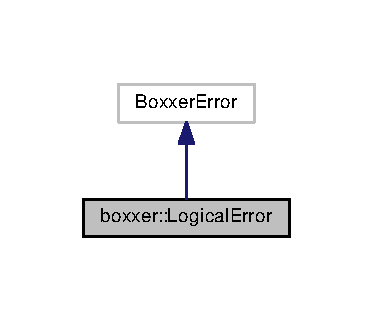
\includegraphics[width=179pt]{structboxxer_1_1LogicalError__inherit__graph}
\end{center}
\end{figure}


Collaboration diagram for boxxer\+:\+:Logical\+Error\+:\nopagebreak
\begin{figure}[H]
\begin{center}
\leavevmode
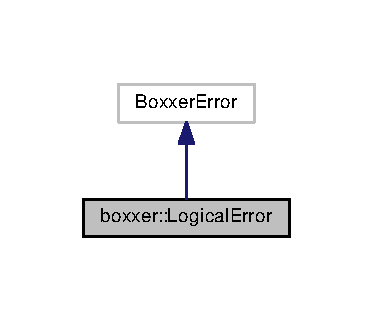
\includegraphics[width=179pt]{structboxxer_1_1LogicalError__coll__graph}
\end{center}
\end{figure}
\subsubsection*{Public Member Functions}
\begin{DoxyCompactItemize}
\item 
\hyperlink{structboxxer_1_1LogicalError_a20a7d64792388f2147ad776528cc2c33}{Logical\+Error} (std\+::string message)
\end{DoxyCompactItemize}


\subsubsection{Detailed Description}
Internal logical error. Bad logic or broken promises. 

Definition at line 32 of file Boxxer\+Error.\+h.



\subsubsection{Constructor \& Destructor Documentation}
\index{boxxer\+::\+Logical\+Error@{boxxer\+::\+Logical\+Error}!Logical\+Error@{Logical\+Error}}
\index{Logical\+Error@{Logical\+Error}!boxxer\+::\+Logical\+Error@{boxxer\+::\+Logical\+Error}}
\paragraph[{\texorpdfstring{Logical\+Error(std\+::string message)}{LogicalError(std::string message)}}]{\setlength{\rightskip}{0pt plus 5cm}boxxer\+::\+Logical\+Error\+::\+Logical\+Error (
\begin{DoxyParamCaption}
\item[{std\+::string}]{message}
\end{DoxyParamCaption}
)\hspace{0.3cm}{\ttfamily [inline]}}\hypertarget{structboxxer_1_1LogicalError_a20a7d64792388f2147ad776528cc2c33}{}\label{structboxxer_1_1LogicalError_a20a7d64792388f2147ad776528cc2c33}


Definition at line 34 of file Boxxer\+Error.\+h.



The documentation for this struct was generated from the following file\+:\begin{DoxyCompactItemize}
\item 
\hyperlink{BoxxerError_8h}{Boxxer\+Error.\+h}\end{DoxyCompactItemize}

\hypertarget{classboxxer_1_1Maxima2D}{}\subsection{boxxer\+:\+:Maxima2D$<$ FloatT, IdxT $>$ Class Template Reference}
\label{classboxxer_1_1Maxima2D}\index{boxxer\+::\+Maxima2\+D$<$ Float\+T, Idx\+T $>$@{boxxer\+::\+Maxima2\+D$<$ Float\+T, Idx\+T $>$}}


{\ttfamily \#include $<$/home/travis/build/markjolah/\+Boxxer/include/\+Boxxer/\+Maxima.\+h$>$}

\subsubsection*{Public Types}
\begin{DoxyCompactItemize}
\item 
using \hyperlink{classboxxer_1_1Maxima2D_a7396e4c9e917dfca02a7763e9f14bd41}{I\+VecT} = arma\+::\+Col$<$ IdxT $>$
\item 
using \hyperlink{classboxxer_1_1Maxima2D_a8b90b97357c1bdf671e833446e15903b}{I\+MatT} = arma\+::\+Mat$<$ IdxT $>$
\item 
using \hyperlink{classboxxer_1_1Maxima2D_a23c658a4a2d6f05fd405d6cdd4f8070b}{VecT} = arma\+::\+Col$<$ FloatT $>$
\item 
using \hyperlink{classboxxer_1_1Maxima2D_ac6ececb6be39bc2fb15904134da4dafb}{ImageT} = arma\+::\+Mat$<$ FloatT $>$
\end{DoxyCompactItemize}
\subsubsection*{Public Member Functions}
\begin{DoxyCompactItemize}
\item 
\hyperlink{classboxxer_1_1Maxima2D_a937ece83a554f957dac931979c58705f}{Maxima2D} (const \hyperlink{classboxxer_1_1Maxima2D_a7396e4c9e917dfca02a7763e9f14bd41}{I\+VecT} \&sizeX, IdxT \hyperlink{classboxxer_1_1Maxima2D_a87d14d6b0d19746a0636204cba3cabfe}{boxsize}=\hyperlink{classboxxer_1_1Maxima2D_ab72858470871c7d5a90ed33839d7f220}{Min\+Boxsize})
\item 
IdxT \hyperlink{classboxxer_1_1Maxima2D_a4fb8ca11caaa1ef72b41673fd32b4db2}{find\+\_\+maxima} (const \hyperlink{classboxxer_1_1Maxima2D_ac6ececb6be39bc2fb15904134da4dafb}{ImageT} \&im)
\item 
IdxT \hyperlink{classboxxer_1_1Maxima2D_adf84d7e78fe730b3f63987af0108a4c0}{find\+\_\+maxima} (const \hyperlink{classboxxer_1_1Maxima2D_ac6ececb6be39bc2fb15904134da4dafb}{ImageT} \&im, \hyperlink{classboxxer_1_1Maxima2D_a8b90b97357c1bdf671e833446e15903b}{I\+MatT} \&maxima\+\_\+out, \hyperlink{classboxxer_1_1Maxima2D_a23c658a4a2d6f05fd405d6cdd4f8070b}{VecT} \&max\+\_\+vals\+\_\+out)
\item 
void \hyperlink{classboxxer_1_1Maxima2D_ac82a58870df8e7ecc1d52f3f4c1bcce1}{read\+\_\+maxima} (IdxT Nmaxima, \hyperlink{classboxxer_1_1Maxima2D_a8b90b97357c1bdf671e833446e15903b}{I\+MatT} \&maxima\+\_\+out, \hyperlink{classboxxer_1_1Maxima2D_a23c658a4a2d6f05fd405d6cdd4f8070b}{VecT} \&max\+\_\+vals\+\_\+out) const 
\item 
void \hyperlink{classboxxer_1_1Maxima2D_a8ec041cd0248571b56015712f4cf6196}{test\+\_\+maxima} (const \hyperlink{classboxxer_1_1Maxima2D_ac6ececb6be39bc2fb15904134da4dafb}{ImageT} \&im)
\item 
bool \hyperlink{classboxxer_1_1Maxima2D_a1a939a9c49eb457a0136ad572c1dce50}{check\+\_\+maxima} (const \hyperlink{classboxxer_1_1Maxima2D_ac6ececb6be39bc2fb15904134da4dafb}{ImageT} \&im, IdxT x, IdxT y, IdxT neigborhood\+Size=\hyperlink{classboxxer_1_1Maxima2D_ab72858470871c7d5a90ed33839d7f220}{Min\+Boxsize})
\end{DoxyCompactItemize}
\subsubsection*{Public Attributes}
\begin{DoxyCompactItemize}
\item 
\hyperlink{classboxxer_1_1Maxima2D_a7396e4c9e917dfca02a7763e9f14bd41}{I\+VecT} \hyperlink{classboxxer_1_1Maxima2D_aa05d0c7a4c0e6ed2b2b918986d53d069}{size}
\item 
IdxT \hyperlink{classboxxer_1_1Maxima2D_a87d14d6b0d19746a0636204cba3cabfe}{boxsize}
\end{DoxyCompactItemize}
\subsubsection*{Static Public Attributes}
\begin{DoxyCompactItemize}
\item 
static const IdxT \hyperlink{classboxxer_1_1Maxima2D_ab72858470871c7d5a90ed33839d7f220}{Min\+Boxsize}
\item 
static const IdxT \hyperlink{classboxxer_1_1Maxima2D_a839c84a80b49cd0bfae1715a04a45ddb}{Ndim}
\end{DoxyCompactItemize}


\subsubsection{Detailed Description}
\subsubsection*{template$<$class FloatT = float, class IdxT = uint32\+\_\+t$>$\\*
class boxxer\+::\+Maxima2\+D$<$ Float\+T, Idx\+T $>$}



Definition at line 16 of file Maxima.\+h.



\subsubsection{Member Typedef Documentation}
\index{boxxer\+::\+Maxima2D@{boxxer\+::\+Maxima2D}!ImageT@{ImageT}}
\index{ImageT@{ImageT}!boxxer\+::\+Maxima2D@{boxxer\+::\+Maxima2D}}
\paragraph[{\texorpdfstring{ImageT}{ImageT}}]{\setlength{\rightskip}{0pt plus 5cm}template$<$class FloatT  = float, class IdxT  = uint32\+\_\+t$>$ using {\bf boxxer\+::\+Maxima2D}$<$ FloatT, IdxT $>$\+::{\bf ImageT} =  arma\+::\+Mat$<$FloatT$>$}\hypertarget{classboxxer_1_1Maxima2D_ac6ececb6be39bc2fb15904134da4dafb}{}\label{classboxxer_1_1Maxima2D_ac6ececb6be39bc2fb15904134da4dafb}


Definition at line 22 of file Maxima.\+h.

\index{boxxer\+::\+Maxima2D@{boxxer\+::\+Maxima2D}!I\+MatT@{I\+MatT}}
\index{I\+MatT@{I\+MatT}!boxxer\+::\+Maxima2D@{boxxer\+::\+Maxima2D}}
\paragraph[{\texorpdfstring{I\+MatT}{IMatT}}]{\setlength{\rightskip}{0pt plus 5cm}template$<$class FloatT  = float, class IdxT  = uint32\+\_\+t$>$ using {\bf boxxer\+::\+Maxima2D}$<$ FloatT, IdxT $>$\+::{\bf I\+MatT} =  arma\+::\+Mat$<$IdxT$>$}\hypertarget{classboxxer_1_1Maxima2D_a8b90b97357c1bdf671e833446e15903b}{}\label{classboxxer_1_1Maxima2D_a8b90b97357c1bdf671e833446e15903b}


Definition at line 20 of file Maxima.\+h.

\index{boxxer\+::\+Maxima2D@{boxxer\+::\+Maxima2D}!I\+VecT@{I\+VecT}}
\index{I\+VecT@{I\+VecT}!boxxer\+::\+Maxima2D@{boxxer\+::\+Maxima2D}}
\paragraph[{\texorpdfstring{I\+VecT}{IVecT}}]{\setlength{\rightskip}{0pt plus 5cm}template$<$class FloatT  = float, class IdxT  = uint32\+\_\+t$>$ using {\bf boxxer\+::\+Maxima2D}$<$ FloatT, IdxT $>$\+::{\bf I\+VecT} =  arma\+::\+Col$<$IdxT$>$}\hypertarget{classboxxer_1_1Maxima2D_a7396e4c9e917dfca02a7763e9f14bd41}{}\label{classboxxer_1_1Maxima2D_a7396e4c9e917dfca02a7763e9f14bd41}


Definition at line 19 of file Maxima.\+h.

\index{boxxer\+::\+Maxima2D@{boxxer\+::\+Maxima2D}!VecT@{VecT}}
\index{VecT@{VecT}!boxxer\+::\+Maxima2D@{boxxer\+::\+Maxima2D}}
\paragraph[{\texorpdfstring{VecT}{VecT}}]{\setlength{\rightskip}{0pt plus 5cm}template$<$class FloatT  = float, class IdxT  = uint32\+\_\+t$>$ using {\bf boxxer\+::\+Maxima2D}$<$ FloatT, IdxT $>$\+::{\bf VecT} =  arma\+::\+Col$<$FloatT$>$}\hypertarget{classboxxer_1_1Maxima2D_a23c658a4a2d6f05fd405d6cdd4f8070b}{}\label{classboxxer_1_1Maxima2D_a23c658a4a2d6f05fd405d6cdd4f8070b}


Definition at line 21 of file Maxima.\+h.



\subsubsection{Constructor \& Destructor Documentation}
\index{boxxer\+::\+Maxima2D@{boxxer\+::\+Maxima2D}!Maxima2D@{Maxima2D}}
\index{Maxima2D@{Maxima2D}!boxxer\+::\+Maxima2D@{boxxer\+::\+Maxima2D}}
\paragraph[{\texorpdfstring{Maxima2\+D(const I\+Vec\+T \&size\+X, Idx\+T boxsize=\+Min\+Boxsize)}{Maxima2D(const IVecT &sizeX, IdxT boxsize=MinBoxsize)}}]{\setlength{\rightskip}{0pt plus 5cm}template$<$class FloatT  = float, class IdxT  = uint32\+\_\+t$>$ {\bf boxxer\+::\+Maxima2D}$<$ FloatT, IdxT $>$\+::{\bf Maxima2D} (
\begin{DoxyParamCaption}
\item[{const {\bf I\+VecT} \&}]{sizeX, }
\item[{IdxT}]{boxsize = {\ttfamily {\bf Min\+Boxsize}}}
\end{DoxyParamCaption}
)}\hypertarget{classboxxer_1_1Maxima2D_a937ece83a554f957dac931979c58705f}{}\label{classboxxer_1_1Maxima2D_a937ece83a554f957dac931979c58705f}


\subsubsection{Member Function Documentation}
\index{boxxer\+::\+Maxima2D@{boxxer\+::\+Maxima2D}!check\+\_\+maxima@{check\+\_\+maxima}}
\index{check\+\_\+maxima@{check\+\_\+maxima}!boxxer\+::\+Maxima2D@{boxxer\+::\+Maxima2D}}
\paragraph[{\texorpdfstring{check\+\_\+maxima(const Image\+T \&im, Idx\+T x, Idx\+T y, Idx\+T neigborhood\+Size=\+Min\+Boxsize)}{check_maxima(const ImageT &im, IdxT x, IdxT y, IdxT neigborhoodSize=MinBoxsize)}}]{\setlength{\rightskip}{0pt plus 5cm}template$<$class FloatT  = float, class IdxT  = uint32\+\_\+t$>$ bool {\bf boxxer\+::\+Maxima2D}$<$ FloatT, IdxT $>$\+::check\+\_\+maxima (
\begin{DoxyParamCaption}
\item[{const {\bf ImageT} \&}]{im, }
\item[{IdxT}]{x, }
\item[{IdxT}]{y, }
\item[{IdxT}]{neigborhood\+Size = {\ttfamily {\bf Min\+Boxsize}}}
\end{DoxyParamCaption}
)}\hypertarget{classboxxer_1_1Maxima2D_a1a939a9c49eb457a0136ad572c1dce50}{}\label{classboxxer_1_1Maxima2D_a1a939a9c49eb457a0136ad572c1dce50}
\index{boxxer\+::\+Maxima2D@{boxxer\+::\+Maxima2D}!find\+\_\+maxima@{find\+\_\+maxima}}
\index{find\+\_\+maxima@{find\+\_\+maxima}!boxxer\+::\+Maxima2D@{boxxer\+::\+Maxima2D}}
\paragraph[{\texorpdfstring{find\+\_\+maxima(const Image\+T \&im)}{find_maxima(const ImageT &im)}}]{\setlength{\rightskip}{0pt plus 5cm}template$<$class FloatT  = float, class IdxT  = uint32\+\_\+t$>$ IdxT {\bf boxxer\+::\+Maxima2D}$<$ FloatT, IdxT $>$\+::find\+\_\+maxima (
\begin{DoxyParamCaption}
\item[{const {\bf ImageT} \&}]{im}
\end{DoxyParamCaption}
)}\hypertarget{classboxxer_1_1Maxima2D_a4fb8ca11caaa1ef72b41673fd32b4db2}{}\label{classboxxer_1_1Maxima2D_a4fb8ca11caaa1ef72b41673fd32b4db2}
\index{boxxer\+::\+Maxima2D@{boxxer\+::\+Maxima2D}!find\+\_\+maxima@{find\+\_\+maxima}}
\index{find\+\_\+maxima@{find\+\_\+maxima}!boxxer\+::\+Maxima2D@{boxxer\+::\+Maxima2D}}
\paragraph[{\texorpdfstring{find\+\_\+maxima(const Image\+T \&im, I\+Mat\+T \&maxima\+\_\+out, Vec\+T \&max\+\_\+vals\+\_\+out)}{find_maxima(const ImageT &im, IMatT &maxima_out, VecT &max_vals_out)}}]{\setlength{\rightskip}{0pt plus 5cm}template$<$class FloatT  = float, class IdxT  = uint32\+\_\+t$>$ IdxT {\bf boxxer\+::\+Maxima2D}$<$ FloatT, IdxT $>$\+::find\+\_\+maxima (
\begin{DoxyParamCaption}
\item[{const {\bf ImageT} \&}]{im, }
\item[{{\bf I\+MatT} \&}]{maxima\+\_\+out, }
\item[{{\bf VecT} \&}]{max\+\_\+vals\+\_\+out}
\end{DoxyParamCaption}
)}\hypertarget{classboxxer_1_1Maxima2D_adf84d7e78fe730b3f63987af0108a4c0}{}\label{classboxxer_1_1Maxima2D_adf84d7e78fe730b3f63987af0108a4c0}
\index{boxxer\+::\+Maxima2D@{boxxer\+::\+Maxima2D}!read\+\_\+maxima@{read\+\_\+maxima}}
\index{read\+\_\+maxima@{read\+\_\+maxima}!boxxer\+::\+Maxima2D@{boxxer\+::\+Maxima2D}}
\paragraph[{\texorpdfstring{read\+\_\+maxima(\+Idx\+T Nmaxima, I\+Mat\+T \&maxima\+\_\+out, Vec\+T \&max\+\_\+vals\+\_\+out) const }{read_maxima(IdxT Nmaxima, IMatT &maxima_out, VecT &max_vals_out) const }}]{\setlength{\rightskip}{0pt plus 5cm}template$<$class FloatT  = float, class IdxT  = uint32\+\_\+t$>$ void {\bf boxxer\+::\+Maxima2D}$<$ FloatT, IdxT $>$\+::read\+\_\+maxima (
\begin{DoxyParamCaption}
\item[{IdxT}]{Nmaxima, }
\item[{{\bf I\+MatT} \&}]{maxima\+\_\+out, }
\item[{{\bf VecT} \&}]{max\+\_\+vals\+\_\+out}
\end{DoxyParamCaption}
) const}\hypertarget{classboxxer_1_1Maxima2D_ac82a58870df8e7ecc1d52f3f4c1bcce1}{}\label{classboxxer_1_1Maxima2D_ac82a58870df8e7ecc1d52f3f4c1bcce1}
\index{boxxer\+::\+Maxima2D@{boxxer\+::\+Maxima2D}!test\+\_\+maxima@{test\+\_\+maxima}}
\index{test\+\_\+maxima@{test\+\_\+maxima}!boxxer\+::\+Maxima2D@{boxxer\+::\+Maxima2D}}
\paragraph[{\texorpdfstring{test\+\_\+maxima(const Image\+T \&im)}{test_maxima(const ImageT &im)}}]{\setlength{\rightskip}{0pt plus 5cm}template$<$class FloatT  = float, class IdxT  = uint32\+\_\+t$>$ void {\bf boxxer\+::\+Maxima2D}$<$ FloatT, IdxT $>$\+::test\+\_\+maxima (
\begin{DoxyParamCaption}
\item[{const {\bf ImageT} \&}]{im}
\end{DoxyParamCaption}
)}\hypertarget{classboxxer_1_1Maxima2D_a8ec041cd0248571b56015712f4cf6196}{}\label{classboxxer_1_1Maxima2D_a8ec041cd0248571b56015712f4cf6196}


\subsubsection{Member Data Documentation}
\index{boxxer\+::\+Maxima2D@{boxxer\+::\+Maxima2D}!boxsize@{boxsize}}
\index{boxsize@{boxsize}!boxxer\+::\+Maxima2D@{boxxer\+::\+Maxima2D}}
\paragraph[{\texorpdfstring{boxsize}{boxsize}}]{\setlength{\rightskip}{0pt plus 5cm}template$<$class FloatT  = float, class IdxT  = uint32\+\_\+t$>$ IdxT {\bf boxxer\+::\+Maxima2D}$<$ FloatT, IdxT $>$\+::boxsize}\hypertarget{classboxxer_1_1Maxima2D_a87d14d6b0d19746a0636204cba3cabfe}{}\label{classboxxer_1_1Maxima2D_a87d14d6b0d19746a0636204cba3cabfe}


Definition at line 27 of file Maxima.\+h.

\index{boxxer\+::\+Maxima2D@{boxxer\+::\+Maxima2D}!Min\+Boxsize@{Min\+Boxsize}}
\index{Min\+Boxsize@{Min\+Boxsize}!boxxer\+::\+Maxima2D@{boxxer\+::\+Maxima2D}}
\paragraph[{\texorpdfstring{Min\+Boxsize}{MinBoxsize}}]{\setlength{\rightskip}{0pt plus 5cm}template$<$class FloatT  = float, class IdxT  = uint32\+\_\+t$>$ const IdxT {\bf boxxer\+::\+Maxima2D}$<$ FloatT, IdxT $>$\+::Min\+Boxsize\hspace{0.3cm}{\ttfamily [static]}}\hypertarget{classboxxer_1_1Maxima2D_ab72858470871c7d5a90ed33839d7f220}{}\label{classboxxer_1_1Maxima2D_ab72858470871c7d5a90ed33839d7f220}


Definition at line 23 of file Maxima.\+h.

\index{boxxer\+::\+Maxima2D@{boxxer\+::\+Maxima2D}!Ndim@{Ndim}}
\index{Ndim@{Ndim}!boxxer\+::\+Maxima2D@{boxxer\+::\+Maxima2D}}
\paragraph[{\texorpdfstring{Ndim}{Ndim}}]{\setlength{\rightskip}{0pt plus 5cm}template$<$class FloatT  = float, class IdxT  = uint32\+\_\+t$>$ const IdxT {\bf boxxer\+::\+Maxima2D}$<$ FloatT, IdxT $>$\+::Ndim\hspace{0.3cm}{\ttfamily [static]}}\hypertarget{classboxxer_1_1Maxima2D_a839c84a80b49cd0bfae1715a04a45ddb}{}\label{classboxxer_1_1Maxima2D_a839c84a80b49cd0bfae1715a04a45ddb}


Definition at line 24 of file Maxima.\+h.

\index{boxxer\+::\+Maxima2D@{boxxer\+::\+Maxima2D}!size@{size}}
\index{size@{size}!boxxer\+::\+Maxima2D@{boxxer\+::\+Maxima2D}}
\paragraph[{\texorpdfstring{size}{size}}]{\setlength{\rightskip}{0pt plus 5cm}template$<$class FloatT  = float, class IdxT  = uint32\+\_\+t$>$ {\bf I\+VecT} {\bf boxxer\+::\+Maxima2D}$<$ FloatT, IdxT $>$\+::size}\hypertarget{classboxxer_1_1Maxima2D_aa05d0c7a4c0e6ed2b2b918986d53d069}{}\label{classboxxer_1_1Maxima2D_aa05d0c7a4c0e6ed2b2b918986d53d069}


Definition at line 26 of file Maxima.\+h.



The documentation for this class was generated from the following file\+:\begin{DoxyCompactItemize}
\item 
\hyperlink{Maxima_8h}{Maxima.\+h}\end{DoxyCompactItemize}

\hypertarget{classboxxer_1_1Maxima3D}{}\subsection{boxxer\+:\+:Maxima3D$<$ FloatT, IdxT $>$ Class Template Reference}
\label{classboxxer_1_1Maxima3D}\index{boxxer\+::\+Maxima3\+D$<$ Float\+T, Idx\+T $>$@{boxxer\+::\+Maxima3\+D$<$ Float\+T, Idx\+T $>$}}


{\ttfamily \#include $<$/home/travis/build/markjolah/\+Boxxer/include/\+Boxxer/\+Maxima.\+h$>$}

\subsubsection*{Public Types}
\begin{DoxyCompactItemize}
\item 
using \hyperlink{classboxxer_1_1Maxima3D_a5fee3acd26edc152ba90e90812e40c1f}{I\+VecT} = arma\+::\+Col$<$ IdxT $>$
\item 
using \hyperlink{classboxxer_1_1Maxima3D_a51dcfe38a24fa1264aabbc4369d795bb}{I\+MatT} = arma\+::\+Mat$<$ IdxT $>$
\item 
using \hyperlink{classboxxer_1_1Maxima3D_af84c08251794d634d33f2b388d465724}{I\+CubeT} = arma\+::\+Cube$<$ IdxT $>$
\item 
using \hyperlink{classboxxer_1_1Maxima3D_a3b589b4792d6446b7418a565314b126b}{VecT} = arma\+::\+Col$<$ FloatT $>$
\item 
using \hyperlink{classboxxer_1_1Maxima3D_aebf2125d25bccd44361a369831600569}{ImageT} = arma\+::\+Cube$<$ FloatT $>$
\end{DoxyCompactItemize}
\subsubsection*{Public Member Functions}
\begin{DoxyCompactItemize}
\item 
\hyperlink{classboxxer_1_1Maxima3D_abec4b44770198fd079c0c84a8e418ec9}{Maxima3D} (const \hyperlink{classboxxer_1_1Maxima3D_a5fee3acd26edc152ba90e90812e40c1f}{I\+VecT} \&\hyperlink{classboxxer_1_1Maxima3D_a71f401fe66798eeeb8581faa5f9e0927}{size}, IdxT \hyperlink{classboxxer_1_1Maxima3D_a2902bed080ed07e6409e540f0bb82c34}{boxsize}=\hyperlink{classboxxer_1_1Maxima3D_a31e443fae0ba2fec7cdaebee0d207f31}{Min\+Boxsize})
\item 
IdxT \hyperlink{classboxxer_1_1Maxima3D_ad30559dd64e36cad467d0faa7e3db33c}{find\+\_\+maxima} (const \hyperlink{classboxxer_1_1Maxima3D_aebf2125d25bccd44361a369831600569}{ImageT} \&im)
\item 
IdxT \hyperlink{classboxxer_1_1Maxima3D_ad4ad309b255fc5b04730a8c40d068473}{find\+\_\+maxima} (const \hyperlink{classboxxer_1_1Maxima3D_aebf2125d25bccd44361a369831600569}{ImageT} \&im, \hyperlink{classboxxer_1_1Maxima3D_a51dcfe38a24fa1264aabbc4369d795bb}{I\+MatT} \&maxima\+\_\+out, \hyperlink{classboxxer_1_1Maxima3D_a3b589b4792d6446b7418a565314b126b}{VecT} \&max\+\_\+vals\+\_\+out)
\item 
void \hyperlink{classboxxer_1_1Maxima3D_a3a2f1e54987e235f59e2f1c1af5b2614}{read\+\_\+maxima} (\hyperlink{classboxxer_1_1Maxima3D_a51dcfe38a24fa1264aabbc4369d795bb}{I\+MatT} \&maxima\+\_\+out, \hyperlink{classboxxer_1_1Maxima3D_a3b589b4792d6446b7418a565314b126b}{VecT} \&max\+\_\+vals\+\_\+out) const 
\item 
void \hyperlink{classboxxer_1_1Maxima3D_a1057e4adf9dbb6410bc246648ae7d4bb}{test\+\_\+maxima} (const \hyperlink{classboxxer_1_1Maxima3D_aebf2125d25bccd44361a369831600569}{ImageT} \&im)
\item 
bool \hyperlink{classboxxer_1_1Maxima3D_ae01e8a792ba04cefd5d8abbaf40bb669}{check\+\_\+maxima} (const \hyperlink{classboxxer_1_1Maxima3D_aebf2125d25bccd44361a369831600569}{ImageT} \&im, IdxT x, IdxT y, IdxT z, IdxT neigborhood\+Size=\hyperlink{classboxxer_1_1Maxima3D_a31e443fae0ba2fec7cdaebee0d207f31}{Min\+Boxsize})
\end{DoxyCompactItemize}
\subsubsection*{Public Attributes}
\begin{DoxyCompactItemize}
\item 
\hyperlink{classboxxer_1_1Maxima3D_a5fee3acd26edc152ba90e90812e40c1f}{I\+VecT} \hyperlink{classboxxer_1_1Maxima3D_a71f401fe66798eeeb8581faa5f9e0927}{size}
\item 
IdxT \hyperlink{classboxxer_1_1Maxima3D_a2902bed080ed07e6409e540f0bb82c34}{boxsize}
\end{DoxyCompactItemize}
\subsubsection*{Static Public Attributes}
\begin{DoxyCompactItemize}
\item 
static const IdxT \hyperlink{classboxxer_1_1Maxima3D_a31e443fae0ba2fec7cdaebee0d207f31}{Min\+Boxsize}
\item 
static const IdxT \hyperlink{classboxxer_1_1Maxima3D_ae446af4adb99b87f2211f3b4d83b6273}{Ndim}
\end{DoxyCompactItemize}


\subsubsection{Detailed Description}
\subsubsection*{template$<$class FloatT = float, class IdxT = uint32\+\_\+t$>$\\*
class boxxer\+::\+Maxima3\+D$<$ Float\+T, Idx\+T $>$}



Definition at line 52 of file Maxima.\+h.



\subsubsection{Member Typedef Documentation}
\index{boxxer\+::\+Maxima3D@{boxxer\+::\+Maxima3D}!I\+CubeT@{I\+CubeT}}
\index{I\+CubeT@{I\+CubeT}!boxxer\+::\+Maxima3D@{boxxer\+::\+Maxima3D}}
\paragraph[{\texorpdfstring{I\+CubeT}{ICubeT}}]{\setlength{\rightskip}{0pt plus 5cm}template$<$class FloatT  = float, class IdxT  = uint32\+\_\+t$>$ using {\bf boxxer\+::\+Maxima3D}$<$ FloatT, IdxT $>$\+::{\bf I\+CubeT} =  arma\+::\+Cube$<$IdxT$>$}\hypertarget{classboxxer_1_1Maxima3D_af84c08251794d634d33f2b388d465724}{}\label{classboxxer_1_1Maxima3D_af84c08251794d634d33f2b388d465724}


Definition at line 57 of file Maxima.\+h.

\index{boxxer\+::\+Maxima3D@{boxxer\+::\+Maxima3D}!ImageT@{ImageT}}
\index{ImageT@{ImageT}!boxxer\+::\+Maxima3D@{boxxer\+::\+Maxima3D}}
\paragraph[{\texorpdfstring{ImageT}{ImageT}}]{\setlength{\rightskip}{0pt plus 5cm}template$<$class FloatT  = float, class IdxT  = uint32\+\_\+t$>$ using {\bf boxxer\+::\+Maxima3D}$<$ FloatT, IdxT $>$\+::{\bf ImageT} =  arma\+::\+Cube$<$FloatT$>$}\hypertarget{classboxxer_1_1Maxima3D_aebf2125d25bccd44361a369831600569}{}\label{classboxxer_1_1Maxima3D_aebf2125d25bccd44361a369831600569}


Definition at line 59 of file Maxima.\+h.

\index{boxxer\+::\+Maxima3D@{boxxer\+::\+Maxima3D}!I\+MatT@{I\+MatT}}
\index{I\+MatT@{I\+MatT}!boxxer\+::\+Maxima3D@{boxxer\+::\+Maxima3D}}
\paragraph[{\texorpdfstring{I\+MatT}{IMatT}}]{\setlength{\rightskip}{0pt plus 5cm}template$<$class FloatT  = float, class IdxT  = uint32\+\_\+t$>$ using {\bf boxxer\+::\+Maxima3D}$<$ FloatT, IdxT $>$\+::{\bf I\+MatT} =  arma\+::\+Mat$<$IdxT$>$}\hypertarget{classboxxer_1_1Maxima3D_a51dcfe38a24fa1264aabbc4369d795bb}{}\label{classboxxer_1_1Maxima3D_a51dcfe38a24fa1264aabbc4369d795bb}


Definition at line 56 of file Maxima.\+h.

\index{boxxer\+::\+Maxima3D@{boxxer\+::\+Maxima3D}!I\+VecT@{I\+VecT}}
\index{I\+VecT@{I\+VecT}!boxxer\+::\+Maxima3D@{boxxer\+::\+Maxima3D}}
\paragraph[{\texorpdfstring{I\+VecT}{IVecT}}]{\setlength{\rightskip}{0pt plus 5cm}template$<$class FloatT  = float, class IdxT  = uint32\+\_\+t$>$ using {\bf boxxer\+::\+Maxima3D}$<$ FloatT, IdxT $>$\+::{\bf I\+VecT} =  arma\+::\+Col$<$IdxT$>$}\hypertarget{classboxxer_1_1Maxima3D_a5fee3acd26edc152ba90e90812e40c1f}{}\label{classboxxer_1_1Maxima3D_a5fee3acd26edc152ba90e90812e40c1f}


Definition at line 55 of file Maxima.\+h.

\index{boxxer\+::\+Maxima3D@{boxxer\+::\+Maxima3D}!VecT@{VecT}}
\index{VecT@{VecT}!boxxer\+::\+Maxima3D@{boxxer\+::\+Maxima3D}}
\paragraph[{\texorpdfstring{VecT}{VecT}}]{\setlength{\rightskip}{0pt plus 5cm}template$<$class FloatT  = float, class IdxT  = uint32\+\_\+t$>$ using {\bf boxxer\+::\+Maxima3D}$<$ FloatT, IdxT $>$\+::{\bf VecT} =  arma\+::\+Col$<$FloatT$>$}\hypertarget{classboxxer_1_1Maxima3D_a3b589b4792d6446b7418a565314b126b}{}\label{classboxxer_1_1Maxima3D_a3b589b4792d6446b7418a565314b126b}


Definition at line 58 of file Maxima.\+h.



\subsubsection{Constructor \& Destructor Documentation}
\index{boxxer\+::\+Maxima3D@{boxxer\+::\+Maxima3D}!Maxima3D@{Maxima3D}}
\index{Maxima3D@{Maxima3D}!boxxer\+::\+Maxima3D@{boxxer\+::\+Maxima3D}}
\paragraph[{\texorpdfstring{Maxima3\+D(const I\+Vec\+T \&size, Idx\+T boxsize=\+Min\+Boxsize)}{Maxima3D(const IVecT &size, IdxT boxsize=MinBoxsize)}}]{\setlength{\rightskip}{0pt plus 5cm}template$<$class FloatT  = float, class IdxT  = uint32\+\_\+t$>$ {\bf boxxer\+::\+Maxima3D}$<$ FloatT, IdxT $>$\+::{\bf Maxima3D} (
\begin{DoxyParamCaption}
\item[{const {\bf I\+VecT} \&}]{size, }
\item[{IdxT}]{boxsize = {\ttfamily {\bf Min\+Boxsize}}}
\end{DoxyParamCaption}
)}\hypertarget{classboxxer_1_1Maxima3D_abec4b44770198fd079c0c84a8e418ec9}{}\label{classboxxer_1_1Maxima3D_abec4b44770198fd079c0c84a8e418ec9}


\subsubsection{Member Function Documentation}
\index{boxxer\+::\+Maxima3D@{boxxer\+::\+Maxima3D}!check\+\_\+maxima@{check\+\_\+maxima}}
\index{check\+\_\+maxima@{check\+\_\+maxima}!boxxer\+::\+Maxima3D@{boxxer\+::\+Maxima3D}}
\paragraph[{\texorpdfstring{check\+\_\+maxima(const Image\+T \&im, Idx\+T x, Idx\+T y, Idx\+T z, Idx\+T neigborhood\+Size=\+Min\+Boxsize)}{check_maxima(const ImageT &im, IdxT x, IdxT y, IdxT z, IdxT neigborhoodSize=MinBoxsize)}}]{\setlength{\rightskip}{0pt plus 5cm}template$<$class FloatT  = float, class IdxT  = uint32\+\_\+t$>$ bool {\bf boxxer\+::\+Maxima3D}$<$ FloatT, IdxT $>$\+::check\+\_\+maxima (
\begin{DoxyParamCaption}
\item[{const {\bf ImageT} \&}]{im, }
\item[{IdxT}]{x, }
\item[{IdxT}]{y, }
\item[{IdxT}]{z, }
\item[{IdxT}]{neigborhood\+Size = {\ttfamily {\bf Min\+Boxsize}}}
\end{DoxyParamCaption}
)}\hypertarget{classboxxer_1_1Maxima3D_ae01e8a792ba04cefd5d8abbaf40bb669}{}\label{classboxxer_1_1Maxima3D_ae01e8a792ba04cefd5d8abbaf40bb669}
\index{boxxer\+::\+Maxima3D@{boxxer\+::\+Maxima3D}!find\+\_\+maxima@{find\+\_\+maxima}}
\index{find\+\_\+maxima@{find\+\_\+maxima}!boxxer\+::\+Maxima3D@{boxxer\+::\+Maxima3D}}
\paragraph[{\texorpdfstring{find\+\_\+maxima(const Image\+T \&im)}{find_maxima(const ImageT &im)}}]{\setlength{\rightskip}{0pt plus 5cm}template$<$class FloatT  = float, class IdxT  = uint32\+\_\+t$>$ IdxT {\bf boxxer\+::\+Maxima3D}$<$ FloatT, IdxT $>$\+::find\+\_\+maxima (
\begin{DoxyParamCaption}
\item[{const {\bf ImageT} \&}]{im}
\end{DoxyParamCaption}
)}\hypertarget{classboxxer_1_1Maxima3D_ad30559dd64e36cad467d0faa7e3db33c}{}\label{classboxxer_1_1Maxima3D_ad30559dd64e36cad467d0faa7e3db33c}
\index{boxxer\+::\+Maxima3D@{boxxer\+::\+Maxima3D}!find\+\_\+maxima@{find\+\_\+maxima}}
\index{find\+\_\+maxima@{find\+\_\+maxima}!boxxer\+::\+Maxima3D@{boxxer\+::\+Maxima3D}}
\paragraph[{\texorpdfstring{find\+\_\+maxima(const Image\+T \&im, I\+Mat\+T \&maxima\+\_\+out, Vec\+T \&max\+\_\+vals\+\_\+out)}{find_maxima(const ImageT &im, IMatT &maxima_out, VecT &max_vals_out)}}]{\setlength{\rightskip}{0pt plus 5cm}template$<$class FloatT  = float, class IdxT  = uint32\+\_\+t$>$ IdxT {\bf boxxer\+::\+Maxima3D}$<$ FloatT, IdxT $>$\+::find\+\_\+maxima (
\begin{DoxyParamCaption}
\item[{const {\bf ImageT} \&}]{im, }
\item[{{\bf I\+MatT} \&}]{maxima\+\_\+out, }
\item[{{\bf VecT} \&}]{max\+\_\+vals\+\_\+out}
\end{DoxyParamCaption}
)}\hypertarget{classboxxer_1_1Maxima3D_ad4ad309b255fc5b04730a8c40d068473}{}\label{classboxxer_1_1Maxima3D_ad4ad309b255fc5b04730a8c40d068473}
\index{boxxer\+::\+Maxima3D@{boxxer\+::\+Maxima3D}!read\+\_\+maxima@{read\+\_\+maxima}}
\index{read\+\_\+maxima@{read\+\_\+maxima}!boxxer\+::\+Maxima3D@{boxxer\+::\+Maxima3D}}
\paragraph[{\texorpdfstring{read\+\_\+maxima(\+I\+Mat\+T \&maxima\+\_\+out, Vec\+T \&max\+\_\+vals\+\_\+out) const }{read_maxima(IMatT &maxima_out, VecT &max_vals_out) const }}]{\setlength{\rightskip}{0pt plus 5cm}template$<$class FloatT  = float, class IdxT  = uint32\+\_\+t$>$ void {\bf boxxer\+::\+Maxima3D}$<$ FloatT, IdxT $>$\+::read\+\_\+maxima (
\begin{DoxyParamCaption}
\item[{{\bf I\+MatT} \&}]{maxima\+\_\+out, }
\item[{{\bf VecT} \&}]{max\+\_\+vals\+\_\+out}
\end{DoxyParamCaption}
) const}\hypertarget{classboxxer_1_1Maxima3D_a3a2f1e54987e235f59e2f1c1af5b2614}{}\label{classboxxer_1_1Maxima3D_a3a2f1e54987e235f59e2f1c1af5b2614}
\index{boxxer\+::\+Maxima3D@{boxxer\+::\+Maxima3D}!test\+\_\+maxima@{test\+\_\+maxima}}
\index{test\+\_\+maxima@{test\+\_\+maxima}!boxxer\+::\+Maxima3D@{boxxer\+::\+Maxima3D}}
\paragraph[{\texorpdfstring{test\+\_\+maxima(const Image\+T \&im)}{test_maxima(const ImageT &im)}}]{\setlength{\rightskip}{0pt plus 5cm}template$<$class FloatT  = float, class IdxT  = uint32\+\_\+t$>$ void {\bf boxxer\+::\+Maxima3D}$<$ FloatT, IdxT $>$\+::test\+\_\+maxima (
\begin{DoxyParamCaption}
\item[{const {\bf ImageT} \&}]{im}
\end{DoxyParamCaption}
)}\hypertarget{classboxxer_1_1Maxima3D_a1057e4adf9dbb6410bc246648ae7d4bb}{}\label{classboxxer_1_1Maxima3D_a1057e4adf9dbb6410bc246648ae7d4bb}


\subsubsection{Member Data Documentation}
\index{boxxer\+::\+Maxima3D@{boxxer\+::\+Maxima3D}!boxsize@{boxsize}}
\index{boxsize@{boxsize}!boxxer\+::\+Maxima3D@{boxxer\+::\+Maxima3D}}
\paragraph[{\texorpdfstring{boxsize}{boxsize}}]{\setlength{\rightskip}{0pt plus 5cm}template$<$class FloatT  = float, class IdxT  = uint32\+\_\+t$>$ IdxT {\bf boxxer\+::\+Maxima3D}$<$ FloatT, IdxT $>$\+::boxsize}\hypertarget{classboxxer_1_1Maxima3D_a2902bed080ed07e6409e540f0bb82c34}{}\label{classboxxer_1_1Maxima3D_a2902bed080ed07e6409e540f0bb82c34}


Definition at line 65 of file Maxima.\+h.

\index{boxxer\+::\+Maxima3D@{boxxer\+::\+Maxima3D}!Min\+Boxsize@{Min\+Boxsize}}
\index{Min\+Boxsize@{Min\+Boxsize}!boxxer\+::\+Maxima3D@{boxxer\+::\+Maxima3D}}
\paragraph[{\texorpdfstring{Min\+Boxsize}{MinBoxsize}}]{\setlength{\rightskip}{0pt plus 5cm}template$<$class FloatT  = float, class IdxT  = uint32\+\_\+t$>$ const IdxT {\bf boxxer\+::\+Maxima3D}$<$ FloatT, IdxT $>$\+::Min\+Boxsize\hspace{0.3cm}{\ttfamily [static]}}\hypertarget{classboxxer_1_1Maxima3D_a31e443fae0ba2fec7cdaebee0d207f31}{}\label{classboxxer_1_1Maxima3D_a31e443fae0ba2fec7cdaebee0d207f31}


Definition at line 61 of file Maxima.\+h.

\index{boxxer\+::\+Maxima3D@{boxxer\+::\+Maxima3D}!Ndim@{Ndim}}
\index{Ndim@{Ndim}!boxxer\+::\+Maxima3D@{boxxer\+::\+Maxima3D}}
\paragraph[{\texorpdfstring{Ndim}{Ndim}}]{\setlength{\rightskip}{0pt plus 5cm}template$<$class FloatT  = float, class IdxT  = uint32\+\_\+t$>$ const IdxT {\bf boxxer\+::\+Maxima3D}$<$ FloatT, IdxT $>$\+::Ndim\hspace{0.3cm}{\ttfamily [static]}}\hypertarget{classboxxer_1_1Maxima3D_ae446af4adb99b87f2211f3b4d83b6273}{}\label{classboxxer_1_1Maxima3D_ae446af4adb99b87f2211f3b4d83b6273}


Definition at line 62 of file Maxima.\+h.

\index{boxxer\+::\+Maxima3D@{boxxer\+::\+Maxima3D}!size@{size}}
\index{size@{size}!boxxer\+::\+Maxima3D@{boxxer\+::\+Maxima3D}}
\paragraph[{\texorpdfstring{size}{size}}]{\setlength{\rightskip}{0pt plus 5cm}template$<$class FloatT  = float, class IdxT  = uint32\+\_\+t$>$ {\bf I\+VecT} {\bf boxxer\+::\+Maxima3D}$<$ FloatT, IdxT $>$\+::size}\hypertarget{classboxxer_1_1Maxima3D_a71f401fe66798eeeb8581faa5f9e0927}{}\label{classboxxer_1_1Maxima3D_a71f401fe66798eeeb8581faa5f9e0927}


Definition at line 64 of file Maxima.\+h.



The documentation for this class was generated from the following file\+:\begin{DoxyCompactItemize}
\item 
\hyperlink{Maxima_8h}{Maxima.\+h}\end{DoxyCompactItemize}

\hypertarget{structboxxer_1_1NumericalError}{}\subsection{boxxer\+:\+:Numerical\+Error Struct Reference}
\label{structboxxer_1_1NumericalError}\index{boxxer\+::\+Numerical\+Error@{boxxer\+::\+Numerical\+Error}}


Internal numerical error.  




{\ttfamily \#include $<$/home/travis/build/markjolah/\+Boxxer/include/\+Boxxer/\+Boxxer\+Error.\+h$>$}



Inheritance diagram for boxxer\+:\+:Numerical\+Error\+:\nopagebreak
\begin{figure}[H]
\begin{center}
\leavevmode
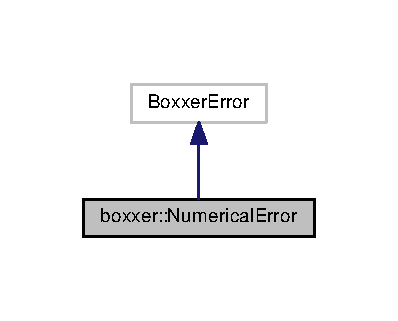
\includegraphics[width=191pt]{structboxxer_1_1NumericalError__inherit__graph}
\end{center}
\end{figure}


Collaboration diagram for boxxer\+:\+:Numerical\+Error\+:\nopagebreak
\begin{figure}[H]
\begin{center}
\leavevmode
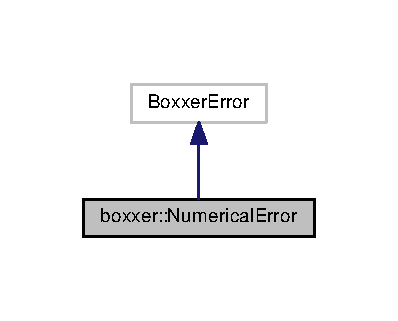
\includegraphics[width=191pt]{structboxxer_1_1NumericalError__coll__graph}
\end{center}
\end{figure}
\subsubsection*{Public Member Functions}
\begin{DoxyCompactItemize}
\item 
\hyperlink{structboxxer_1_1NumericalError_a35fca9d555108f8721314e938004dff5}{Numerical\+Error} (std\+::string message)
\end{DoxyCompactItemize}


\subsubsection{Detailed Description}
Internal numerical error. 

Definition at line 39 of file Boxxer\+Error.\+h.



\subsubsection{Constructor \& Destructor Documentation}
\index{boxxer\+::\+Numerical\+Error@{boxxer\+::\+Numerical\+Error}!Numerical\+Error@{Numerical\+Error}}
\index{Numerical\+Error@{Numerical\+Error}!boxxer\+::\+Numerical\+Error@{boxxer\+::\+Numerical\+Error}}
\paragraph[{\texorpdfstring{Numerical\+Error(std\+::string message)}{NumericalError(std::string message)}}]{\setlength{\rightskip}{0pt plus 5cm}boxxer\+::\+Numerical\+Error\+::\+Numerical\+Error (
\begin{DoxyParamCaption}
\item[{std\+::string}]{message}
\end{DoxyParamCaption}
)\hspace{0.3cm}{\ttfamily [inline]}}\hypertarget{structboxxer_1_1NumericalError_a35fca9d555108f8721314e938004dff5}{}\label{structboxxer_1_1NumericalError_a35fca9d555108f8721314e938004dff5}


Definition at line 41 of file Boxxer\+Error.\+h.



The documentation for this struct was generated from the following file\+:\begin{DoxyCompactItemize}
\item 
\hyperlink{BoxxerError_8h}{Boxxer\+Error.\+h}\end{DoxyCompactItemize}

\hypertarget{structboxxer_1_1ParameterShapeError}{}\subsection{boxxer\+:\+:Parameter\+Shape\+Error Struct Reference}
\label{structboxxer_1_1ParameterShapeError}\index{boxxer\+::\+Parameter\+Shape\+Error@{boxxer\+::\+Parameter\+Shape\+Error}}


Parameters are the incorrect shape, size or number of dimensions.  




{\ttfamily \#include $<$/home/travis/build/markjolah/\+Boxxer/include/\+Boxxer/\+Boxxer\+Error.\+h$>$}



Inheritance diagram for boxxer\+:\+:Parameter\+Shape\+Error\+:\nopagebreak
\begin{figure}[H]
\begin{center}
\leavevmode
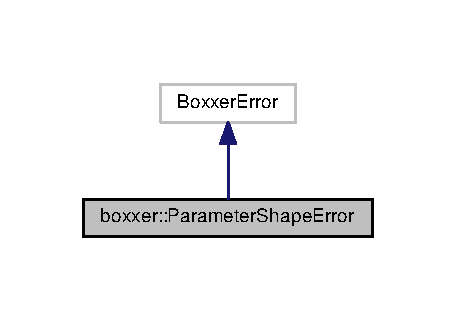
\includegraphics[width=219pt]{structboxxer_1_1ParameterShapeError__inherit__graph}
\end{center}
\end{figure}


Collaboration diagram for boxxer\+:\+:Parameter\+Shape\+Error\+:\nopagebreak
\begin{figure}[H]
\begin{center}
\leavevmode
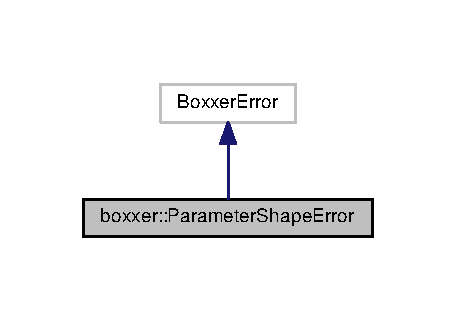
\includegraphics[width=219pt]{structboxxer_1_1ParameterShapeError__coll__graph}
\end{center}
\end{figure}
\subsubsection*{Public Member Functions}
\begin{DoxyCompactItemize}
\item 
\hyperlink{structboxxer_1_1ParameterShapeError_a235b9ef4cacd981438b12e13dff90228}{Parameter\+Shape\+Error} (std\+::string message)
\end{DoxyCompactItemize}


\subsubsection{Detailed Description}
Parameters are the incorrect shape, size or number of dimensions. 

Definition at line 25 of file Boxxer\+Error.\+h.



\subsubsection{Constructor \& Destructor Documentation}
\index{boxxer\+::\+Parameter\+Shape\+Error@{boxxer\+::\+Parameter\+Shape\+Error}!Parameter\+Shape\+Error@{Parameter\+Shape\+Error}}
\index{Parameter\+Shape\+Error@{Parameter\+Shape\+Error}!boxxer\+::\+Parameter\+Shape\+Error@{boxxer\+::\+Parameter\+Shape\+Error}}
\paragraph[{\texorpdfstring{Parameter\+Shape\+Error(std\+::string message)}{ParameterShapeError(std::string message)}}]{\setlength{\rightskip}{0pt plus 5cm}boxxer\+::\+Parameter\+Shape\+Error\+::\+Parameter\+Shape\+Error (
\begin{DoxyParamCaption}
\item[{std\+::string}]{message}
\end{DoxyParamCaption}
)\hspace{0.3cm}{\ttfamily [inline]}}\hypertarget{structboxxer_1_1ParameterShapeError_a235b9ef4cacd981438b12e13dff90228}{}\label{structboxxer_1_1ParameterShapeError_a235b9ef4cacd981438b12e13dff90228}


Definition at line 27 of file Boxxer\+Error.\+h.



The documentation for this struct was generated from the following file\+:\begin{DoxyCompactItemize}
\item 
\hyperlink{BoxxerError_8h}{Boxxer\+Error.\+h}\end{DoxyCompactItemize}

\hypertarget{structboxxer_1_1ParameterValueError}{}\subsection{boxxer\+:\+:Parameter\+Value\+Error Struct Reference}
\label{structboxxer_1_1ParameterValueError}\index{boxxer\+::\+Parameter\+Value\+Error@{boxxer\+::\+Parameter\+Value\+Error}}


Parameter value is not valid.  




{\ttfamily \#include $<$/home/travis/build/markjolah/\+Boxxer/include/\+Boxxer/\+Boxxer\+Error.\+h$>$}



Inheritance diagram for boxxer\+:\+:Parameter\+Value\+Error\+:\nopagebreak
\begin{figure}[H]
\begin{center}
\leavevmode
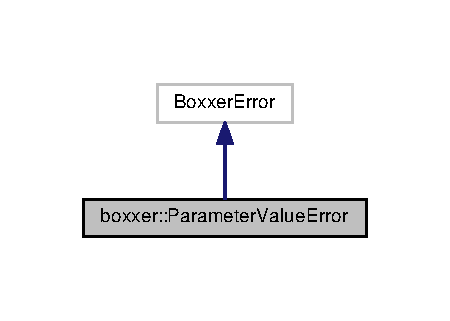
\includegraphics[width=216pt]{structboxxer_1_1ParameterValueError__inherit__graph}
\end{center}
\end{figure}


Collaboration diagram for boxxer\+:\+:Parameter\+Value\+Error\+:\nopagebreak
\begin{figure}[H]
\begin{center}
\leavevmode
\includegraphics[width=216pt]{structboxxer_1_1ParameterValueError__coll__graph}
\end{center}
\end{figure}
\subsubsection*{Public Member Functions}
\begin{DoxyCompactItemize}
\item 
\hyperlink{structboxxer_1_1ParameterValueError_a5683eda75c13e33566d5829ef391302e}{Parameter\+Value\+Error} (std\+::string message)
\end{DoxyCompactItemize}


\subsubsection{Detailed Description}
Parameter value is not valid. 

Definition at line 18 of file Boxxer\+Error.\+h.



\subsubsection{Constructor \& Destructor Documentation}
\index{boxxer\+::\+Parameter\+Value\+Error@{boxxer\+::\+Parameter\+Value\+Error}!Parameter\+Value\+Error@{Parameter\+Value\+Error}}
\index{Parameter\+Value\+Error@{Parameter\+Value\+Error}!boxxer\+::\+Parameter\+Value\+Error@{boxxer\+::\+Parameter\+Value\+Error}}
\paragraph[{\texorpdfstring{Parameter\+Value\+Error(std\+::string message)}{ParameterValueError(std::string message)}}]{\setlength{\rightskip}{0pt plus 5cm}boxxer\+::\+Parameter\+Value\+Error\+::\+Parameter\+Value\+Error (
\begin{DoxyParamCaption}
\item[{std\+::string}]{message}
\end{DoxyParamCaption}
)\hspace{0.3cm}{\ttfamily [inline]}}\hypertarget{structboxxer_1_1ParameterValueError_a5683eda75c13e33566d5829ef391302e}{}\label{structboxxer_1_1ParameterValueError_a5683eda75c13e33566d5829ef391302e}


Definition at line 20 of file Boxxer\+Error.\+h.



The documentation for this struct was generated from the following file\+:\begin{DoxyCompactItemize}
\item 
\hyperlink{BoxxerError_8h}{Boxxer\+Error.\+h}\end{DoxyCompactItemize}

\section{File Documentation}
\hypertarget{Boxxer2D_8h}{}\subsection{Boxxer2\+D.\+h File Reference}
\label{Boxxer2D_8h}\index{Boxxer2\+D.\+h@{Boxxer2\+D.\+h}}


The class declaration for Boxxer2D.  


{\ttfamily \#include $<$cstdint$>$}\\*
{\ttfamily \#include $<$armadillo$>$}\\*
{\ttfamily \#include \char`\"{}Boxxer/\+Hypercube/\+Hypercube.\+h\char`\"{}}\\*
Include dependency graph for Boxxer2\+D.\+h\+:\nopagebreak
\begin{figure}[H]
\begin{center}
\leavevmode
\includegraphics[width=350pt]{Boxxer2D_8h__incl}
\end{center}
\end{figure}
\subsubsection*{Classes}
\begin{DoxyCompactItemize}
\item 
class \hyperlink{classboxxer_1_1Boxxer2D}{boxxer\+::\+Boxxer2\+D$<$ Float\+T, Idx\+T $>$}
\end{DoxyCompactItemize}
\subsubsection*{Namespaces}
\begin{DoxyCompactItemize}
\item 
 \hyperlink{namespaceboxxer}{boxxer}
\end{DoxyCompactItemize}


\subsubsection{Detailed Description}
The class declaration for Boxxer2D. 

\begin{DoxyAuthor}{Author}
Mark J. Olah (mjo@cs.\+unm D\+OT edu) 
\end{DoxyAuthor}
\begin{DoxyDate}{Date}
2014-\/2019 
\end{DoxyDate}

\hypertarget{Boxxer3D_8h}{}\subsection{Boxxer3\+D.\+h File Reference}
\label{Boxxer3D_8h}\index{Boxxer3\+D.\+h@{Boxxer3\+D.\+h}}


The class declaration for Boxxer3D.  


{\ttfamily \#include $<$cstdint$>$}\\*
{\ttfamily \#include $<$armadillo$>$}\\*
{\ttfamily \#include \char`\"{}Boxxer/\+Hypercube/\+Hypercube.\+h\char`\"{}}\\*
Include dependency graph for Boxxer3\+D.\+h\+:\nopagebreak
\begin{figure}[H]
\begin{center}
\leavevmode
\includegraphics[width=350pt]{Boxxer3D_8h__incl}
\end{center}
\end{figure}
\subsubsection*{Classes}
\begin{DoxyCompactItemize}
\item 
class \hyperlink{classboxxer_1_1Boxxer3D}{boxxer\+::\+Boxxer3\+D$<$ Float\+T, Idx\+T $>$}
\end{DoxyCompactItemize}
\subsubsection*{Namespaces}
\begin{DoxyCompactItemize}
\item 
 \hyperlink{namespaceboxxer}{boxxer}
\end{DoxyCompactItemize}


\subsubsection{Detailed Description}
The class declaration for Boxxer3D. 

\begin{DoxyAuthor}{Author}
Mark J. Olah (mjo@cs.\+unm D\+OT edu) 
\end{DoxyAuthor}
\begin{DoxyDate}{Date}
2014-\/2019 
\end{DoxyDate}

\hypertarget{BoxxerError_8h}{}\subsection{Boxxer\+Error.\+h File Reference}
\label{BoxxerError_8h}\index{Boxxer\+Error.\+h@{Boxxer\+Error.\+h}}


Error handling.  


{\ttfamily \#include \char`\"{}Backtrace\+Exception/\+Backtrace\+Exception.\+h\char`\"{}}\\*
Include dependency graph for Boxxer\+Error.\+h\+:\nopagebreak
\begin{figure}[H]
\begin{center}
\leavevmode
\includegraphics[width=187pt]{BoxxerError_8h__incl}
\end{center}
\end{figure}
\subsubsection*{Classes}
\begin{DoxyCompactItemize}
\item 
struct \hyperlink{structboxxer_1_1ParameterValueError}{boxxer\+::\+Parameter\+Value\+Error}
\begin{DoxyCompactList}\small\item\em Parameter value is not valid. \end{DoxyCompactList}\item 
struct \hyperlink{structboxxer_1_1ParameterShapeError}{boxxer\+::\+Parameter\+Shape\+Error}
\begin{DoxyCompactList}\small\item\em Parameters are the incorrect shape, size or number of dimensions. \end{DoxyCompactList}\item 
struct \hyperlink{structboxxer_1_1LogicalError}{boxxer\+::\+Logical\+Error}
\begin{DoxyCompactList}\small\item\em Internal logical error. Bad logic or broken promises. \end{DoxyCompactList}\item 
struct \hyperlink{structboxxer_1_1NumericalError}{boxxer\+::\+Numerical\+Error}
\begin{DoxyCompactList}\small\item\em Internal numerical error. \end{DoxyCompactList}\end{DoxyCompactItemize}
\subsubsection*{Namespaces}
\begin{DoxyCompactItemize}
\item 
 \hyperlink{namespaceboxxer}{boxxer}
\end{DoxyCompactItemize}
\subsubsection*{Typedefs}
\begin{DoxyCompactItemize}
\item 
using \hyperlink{namespaceboxxer_a32d05a7ef7b6f96d0a730455c84e4d31}{boxxer\+::\+Boxxer\+Error} = backtrace\+\_\+exception\+::\+Backtrace\+Exception
\end{DoxyCompactItemize}


\subsubsection{Detailed Description}
Error handling. 

\begin{DoxyAuthor}{Author}
Mark J. Olah (mjo@cs.\+unm D\+OT edu) 
\end{DoxyAuthor}
\begin{DoxyDate}{Date}
2014-\/2019 
\end{DoxyDate}

\hypertarget{FilterKernels_8h}{}\subsection{Filter\+Kernels.\+h File Reference}
\label{FilterKernels_8h}\index{Filter\+Kernels.\+h@{Filter\+Kernels.\+h}}


The \hyperlink{namespaceboxxer_1_1kernels}{boxxer\+::kernels} namespace -\/ low-\/level Gaussian finite-\/impulse response filters.  


{\ttfamily \#include $<$cstdint$>$}\\*
{\ttfamily \#include $<$armadillo$>$}\\*
Include dependency graph for Filter\+Kernels.\+h\+:\nopagebreak
\begin{figure}[H]
\begin{center}
\leavevmode
\includegraphics[width=196pt]{FilterKernels_8h__incl}
\end{center}
\end{figure}
\subsubsection*{Namespaces}
\begin{DoxyCompactItemize}
\item 
 \hyperlink{namespaceboxxer}{boxxer}
\item 
 \hyperlink{namespaceboxxer_1_1kernels}{boxxer\+::kernels}
\end{DoxyCompactItemize}
\subsubsection*{Functions}
\begin{Indent}{\bf 1D Gauss F\+IR Filters}\par
{\em 1D Gaussian finite-\/impulse response filters. }\begin{DoxyCompactItemize}
\item 
{\footnotesize template$<$class FloatT  = float, class IntT  = int32\+\_\+t$>$ }\\void \hyperlink{namespaceboxxer_1_1kernels_aae9636dd5e83f478ed676068c3252627}{boxxer\+::kernels\+::gauss\+F\+I\+R\+\_\+1D} (IntT size, const FloatT data\mbox{[}$\,$\mbox{]}, FloatT fdata\mbox{[}$\,$\mbox{]}, IntT hw, const FloatT kernel\mbox{[}$\,$\mbox{]})
\item 
{\footnotesize template$<$class FloatT  = float, class IntT  = int32\+\_\+t$>$ }\\void \hyperlink{namespaceboxxer_1_1kernels_adf021edf274fc54862b2f9546a47301d}{boxxer\+::kernels\+::gauss\+F\+I\+R\+\_\+1D} (const arma\+::\+Col$<$ FloatT $>$ \&data, arma\+::\+Col$<$ FloatT $>$ \&fdata, const arma\+::\+Col$<$ FloatT $>$ \&kernel)
\item 
{\footnotesize template$<$class FloatT  = float, class IntT  = int32\+\_\+t$>$ }\\void \hyperlink{namespaceboxxer_1_1kernels_af07e73b62933910e86eef6b393155c2c}{boxxer\+::kernels\+::gauss\+F\+I\+R\+\_\+1\+D\+\_\+small} (IntT size, const FloatT data\mbox{[}$\,$\mbox{]}, FloatT fdata\mbox{[}$\,$\mbox{]}, IntT hw, const FloatT kernel\mbox{[}$\,$\mbox{]})
\item 
{\footnotesize template$<$class FloatT  = float, class IntT  = int32\+\_\+t$>$ }\\void \hyperlink{namespaceboxxer_1_1kernels_a88f298ecd82bf9083fabbb2e8a29d4e6}{boxxer\+::kernels\+::gauss\+F\+I\+R\+\_\+1\+D\+\_\+arma} (const arma\+::\+Col$<$ FloatT $>$ \&data, arma\+::\+Col$<$ FloatT $>$ \&fdata, const arma\+::\+Col$<$ FloatT $>$ \&kernel)
\item 
{\footnotesize template$<$class FloatT  = float, class IntT  = int32\+\_\+t$>$ }\\void \hyperlink{namespaceboxxer_1_1kernels_ab2a257fbea765aacf09b558e38637479}{boxxer\+::kernels\+::gauss\+F\+I\+R\+\_\+1\+D\+\_\+inplace\+\_\+arma} (arma\+::\+Col$<$ FloatT $>$ \&data, const arma\+::\+Col$<$ FloatT $>$ \&kernel)
\item 
{\footnotesize template$<$class FloatT  = float, class IntT  = int32\+\_\+t$>$ }\\void \hyperlink{namespaceboxxer_1_1kernels_ab3d9ad7bd61b25b9e856bd0284607e70}{boxxer\+::kernels\+::gauss\+F\+I\+R\+\_\+1\+D\+\_\+inplace} (IntT size, FloatT data\mbox{[}$\,$\mbox{]}, IntT hw, const FloatT kernel\mbox{[}$\,$\mbox{]})
\end{DoxyCompactItemize}
\end{Indent}
\begin{Indent}{\bf 2D Gauss F\+IR Filters}\par
{\em 2D Gaussian finite-\/impulse response filters. }\begin{DoxyCompactItemize}
\item 
{\footnotesize template$<$class FloatT  = float, class IntT  = int32\+\_\+t$>$ }\\void \hyperlink{namespaceboxxer_1_1kernels_aeee9d632ce320eb89c870a44c37efa65}{boxxer\+::kernels\+::gauss\+F\+I\+R\+\_\+2\+Dx} (const arma\+::\+Mat$<$ FloatT $>$ \&data, arma\+::\+Mat$<$ FloatT $>$ \&fdata, const arma\+::\+Col$<$ FloatT $>$ \&kernel)
\item 
{\footnotesize template$<$class FloatT  = float, class IntT  = int32\+\_\+t$>$ }\\void \hyperlink{namespaceboxxer_1_1kernels_a638bf7fa9900937a763f190c0a4499ae}{boxxer\+::kernels\+::gauss\+F\+I\+R\+\_\+2\+Dx\+\_\+small} (const arma\+::\+Mat$<$ FloatT $>$ \&data, arma\+::\+Mat$<$ FloatT $>$ \&fdata, const arma\+::\+Col$<$ FloatT $>$ \&kernel)
\item 
{\footnotesize template$<$class FloatT  = float, class IntT  = int32\+\_\+t$>$ }\\void \hyperlink{namespaceboxxer_1_1kernels_a1da855e7008385fee013bd868d206040}{boxxer\+::kernels\+::gauss\+F\+I\+R\+\_\+2\+Dx\+\_\+arma} (const arma\+::\+Mat$<$ FloatT $>$ \&data, arma\+::\+Mat$<$ FloatT $>$ \&fdata, const arma\+::\+Col$<$ FloatT $>$ \&kernel)
\item 
{\footnotesize template$<$class FloatT  = float, class IntT  = int32\+\_\+t$>$ }\\void \hyperlink{namespaceboxxer_1_1kernels_a6efa0d22ae67955f27c6d9ea30342104}{boxxer\+::kernels\+::gauss\+F\+I\+R\+\_\+2\+Dy} (const arma\+::\+Mat$<$ FloatT $>$ \&data, arma\+::\+Mat$<$ FloatT $>$ \&fdata, const arma\+::\+Col$<$ FloatT $>$ \&kernel)
\item 
{\footnotesize template$<$class FloatT  = float, class IntT  = int32\+\_\+t$>$ }\\void \hyperlink{namespaceboxxer_1_1kernels_aa54bb3fea2d343c030528a87b7916293}{boxxer\+::kernels\+::gauss\+F\+I\+R\+\_\+2\+Dy\+\_\+rowmajor} (const arma\+::\+Mat$<$ FloatT $>$ \&data, arma\+::\+Mat$<$ FloatT $>$ \&fdata, const arma\+::\+Col$<$ FloatT $>$ \&kernel)
\item 
{\footnotesize template$<$class FloatT  = float, class IntT  = int32\+\_\+t$>$ }\\void \hyperlink{namespaceboxxer_1_1kernels_ae78e8767ae044f01e07e61a45220ffc5}{boxxer\+::kernels\+::gauss\+F\+I\+R\+\_\+2\+Dy\+\_\+colmajor} (const arma\+::\+Mat$<$ FloatT $>$ \&data, arma\+::\+Mat$<$ FloatT $>$ \&fdata, const arma\+::\+Col$<$ FloatT $>$ \&kernel)
\item 
{\footnotesize template$<$class FloatT  = float, class IntT  = int32\+\_\+t$>$ }\\void \hyperlink{namespaceboxxer_1_1kernels_a49fd7ed785cfcea57b4c9e67d3113a69}{boxxer\+::kernels\+::gauss\+F\+I\+R\+\_\+2\+Dy\+\_\+small} (const arma\+::\+Mat$<$ FloatT $>$ \&data, arma\+::\+Mat$<$ FloatT $>$ \&fdata, const arma\+::\+Col$<$ FloatT $>$ \&kernel)
\end{DoxyCompactItemize}
\end{Indent}
\begin{Indent}{\bf 3D Gauss F\+IR Filters}\par
{\em 3D Gaussian finite-\/impulse response filters. }\begin{DoxyCompactItemize}
\item 
{\footnotesize template$<$class FloatT  = float, class IntT  = int32\+\_\+t$>$ }\\void \hyperlink{namespaceboxxer_1_1kernels_a74811c999b7d18b14dde0a042318fc06}{boxxer\+::kernels\+::gauss\+F\+I\+R\+\_\+3\+Dx} (const arma\+::\+Cube$<$ FloatT $>$ \&data, arma\+::\+Cube$<$ FloatT $>$ \&fdata, const arma\+::\+Col$<$ FloatT $>$ \&kernel)
\item 
{\footnotesize template$<$class FloatT  = float, class IntT  = int32\+\_\+t$>$ }\\void \hyperlink{namespaceboxxer_1_1kernels_af7d8fb262d8bde9c9907e141c3c5f55f}{boxxer\+::kernels\+::gauss\+F\+I\+R\+\_\+3\+Dx\+\_\+small} (const arma\+::\+Cube$<$ FloatT $>$ \&data, arma\+::\+Cube$<$ FloatT $>$ \&fdata, const arma\+::\+Col$<$ FloatT $>$ \&kernel)
\item 
{\footnotesize template$<$class FloatT  = float, class IntT  = int32\+\_\+t$>$ }\\void \hyperlink{namespaceboxxer_1_1kernels_ac97f85b9211fcffa432b44a86d30c5df}{boxxer\+::kernels\+::gauss\+F\+I\+R\+\_\+3\+Dy} (const arma\+::\+Cube$<$ FloatT $>$ \&data, arma\+::\+Cube$<$ FloatT $>$ \&fdata, const arma\+::\+Col$<$ FloatT $>$ \&kernel)
\item 
{\footnotesize template$<$class FloatT  = float, class IntT  = int32\+\_\+t$>$ }\\void \hyperlink{namespaceboxxer_1_1kernels_a0256b4053077d18bbe2228402071555f}{boxxer\+::kernels\+::gauss\+F\+I\+R\+\_\+3\+Dy\+\_\+small} (const arma\+::\+Cube$<$ FloatT $>$ \&data, arma\+::\+Cube$<$ FloatT $>$ \&fdata, const arma\+::\+Col$<$ FloatT $>$ \&kernel)
\item 
{\footnotesize template$<$class FloatT  = float, class IntT  = int32\+\_\+t$>$ }\\void \hyperlink{namespaceboxxer_1_1kernels_a404ef6e2324a0e4ff53e38ad7b07733e}{boxxer\+::kernels\+::gauss\+F\+I\+R\+\_\+3\+Dz} (const arma\+::\+Cube$<$ FloatT $>$ \&data, arma\+::\+Cube$<$ FloatT $>$ \&fdata, const arma\+::\+Col$<$ FloatT $>$ \&kernel)
\item 
{\footnotesize template$<$class FloatT  = float, class IntT  = int32\+\_\+t$>$ }\\void \hyperlink{namespaceboxxer_1_1kernels_a9a9201ede570bb2d77531d529f39bc99}{boxxer\+::kernels\+::gauss\+F\+I\+R\+\_\+3\+Dz\+\_\+small} (const arma\+::\+Cube$<$ FloatT $>$ \&data, arma\+::\+Cube$<$ FloatT $>$ \&fdata, const arma\+::\+Col$<$ FloatT $>$ \&kernel)
\end{DoxyCompactItemize}
\end{Indent}


\subsubsection{Detailed Description}
The \hyperlink{namespaceboxxer_1_1kernels}{boxxer\+::kernels} namespace -\/ low-\/level Gaussian finite-\/impulse response filters. 

\begin{DoxyAuthor}{Author}
Mark J. Olah (mjo@cs.\+unm D\+OT edu) 
\end{DoxyAuthor}
\begin{DoxyDate}{Date}
2014-\/2019 
\end{DoxyDate}

\hypertarget{GaussFilter_8h}{}\subsection{Gauss\+Filter.\+h File Reference}
\label{GaussFilter_8h}\index{Gauss\+Filter.\+h@{Gauss\+Filter.\+h}}


The class declarations for Gaussian image filter classes.  


{\ttfamily \#include $<$cstdint$>$}\\*
{\ttfamily \#include $<$ostream$>$}\\*
{\ttfamily \#include $<$armadillo$>$}\\*
Include dependency graph for Gauss\+Filter.\+h\+:\nopagebreak
\begin{figure}[H]
\begin{center}
\leavevmode
\includegraphics[width=265pt]{GaussFilter_8h__incl}
\end{center}
\end{figure}
\subsubsection*{Classes}
\begin{DoxyCompactItemize}
\item 
class \hyperlink{classboxxer_1_1GaussFIRFilter}{boxxer\+::\+Gauss\+F\+I\+R\+Filter$<$ Float\+T, Idx\+T $>$}
\item 
class \hyperlink{classboxxer_1_1GaussFilter2D}{boxxer\+::\+Gauss\+Filter2\+D$<$ Float\+T, Idx\+T $>$}
\item 
class \hyperlink{classboxxer_1_1DoGFilter2D}{boxxer\+::\+Do\+G\+Filter2\+D$<$ Float\+T, Idx\+T $>$}
\item 
class \hyperlink{classboxxer_1_1LoGFilter2D}{boxxer\+::\+Lo\+G\+Filter2\+D$<$ Float\+T, Idx\+T $>$}
\item 
class \hyperlink{classboxxer_1_1GaussFilter3D}{boxxer\+::\+Gauss\+Filter3\+D$<$ Float\+T, Idx\+T $>$}
\item 
class \hyperlink{classboxxer_1_1DoGFilter3D}{boxxer\+::\+Do\+G\+Filter3\+D$<$ Float\+T, Idx\+T $>$}
\item 
class \hyperlink{classboxxer_1_1LoGFilter3D}{boxxer\+::\+Lo\+G\+Filter3\+D$<$ Float\+T, Idx\+T $>$}
\end{DoxyCompactItemize}
\subsubsection*{Namespaces}
\begin{DoxyCompactItemize}
\item 
 \hyperlink{namespaceboxxer}{boxxer}
\end{DoxyCompactItemize}


\subsubsection{Detailed Description}
The class declarations for Gaussian image filter classes. 

\begin{DoxyAuthor}{Author}
Mark J. Olah (mjo@cs.\+unm D\+OT edu) 
\end{DoxyAuthor}
\begin{DoxyDate}{Date}
2014-\/2019 These classes are meant to be a per-\/thread worker class or a direct interface for single threaded processes. Each object has its own local storage of which is only 1 or 2 frames in size. 
\end{DoxyDate}

\hypertarget{Maxima_8h}{}\subsection{Maxima.\+h File Reference}
\label{Maxima_8h}\index{Maxima.\+h@{Maxima.\+h}}


The class declaration for the local maxima finders Maxima2D and Maxima3D.  


{\ttfamily \#include $<$cstdint$>$}\\*
{\ttfamily \#include $<$armadillo$>$}\\*
Include dependency graph for Maxima.\+h\+:\nopagebreak
\begin{figure}[H]
\begin{center}
\leavevmode
\includegraphics[width=196pt]{Maxima_8h__incl}
\end{center}
\end{figure}
\subsubsection*{Classes}
\begin{DoxyCompactItemize}
\item 
class \hyperlink{classboxxer_1_1Maxima2D}{boxxer\+::\+Maxima2\+D$<$ Float\+T, Idx\+T $>$}
\item 
class \hyperlink{classboxxer_1_1Maxima3D}{boxxer\+::\+Maxima3\+D$<$ Float\+T, Idx\+T $>$}
\end{DoxyCompactItemize}
\subsubsection*{Namespaces}
\begin{DoxyCompactItemize}
\item 
 \hyperlink{namespaceboxxer}{boxxer}
\end{DoxyCompactItemize}


\subsubsection{Detailed Description}
The class declaration for the local maxima finders Maxima2D and Maxima3D. 

\begin{DoxyAuthor}{Author}
Mark J. Olah (mjo@cs.\+unm D\+OT edu) 
\end{DoxyAuthor}
\begin{DoxyDate}{Date}
2014-\/2019 
\end{DoxyDate}

\hypertarget{README_8md}{}\subsection{R\+E\+A\+D\+M\+E.\+md File Reference}
\label{README_8md}\index{R\+E\+A\+D\+M\+E.\+md@{R\+E\+A\+D\+M\+E.\+md}}

%--- End generated contents ---

% Index
\newpage
\phantomsection
\clearemptydoublepage
\addcontentsline{toc}{section}{Index}
\printindex

\end{document}
